\PassOptionsToPackage{table}{xcolor}
\documentclass{midl}
% MIDL 2027 full paper. Every number in the text is a macro generated by metrics/recompute.py (tables/numbers.tex);
% implementation facts (architectures, settings) are taken from the code (report/code_map_*.md).
\usepackage{booktabs}
\usepackage{adjustbox}
\usepackage{colortbl}
\usepackage{multirow}
\usepackage{amsmath}
\usepackage{bm}
\usepackage{siunitx}
\sisetup{detect-all}
\definecolor{modebest}{HTML}{E8F1FA}
\newcommand{\todo}[1]{\textcolor{red}{[TODO: #1]}}
\newcommand{\mci}[3]{\begin{tabular}[c]{@{}c@{}}#1\\[-1.5pt]{\scriptsize[#2, #3]}\end{tabular}}
\newcommand{\pooledpillarZattn}{0.886}
\newcommand{\pooledpillarZattnthenlorag}{0.900}
\newcommand{\pooledpillarZattnft}{0.922}
\newcommand{\pooledpillarZbabmil}{0.914}
\newcommand{\pooledpillarZdora}{0.921}
\newcommand{\pooledpillarZfullft}{0.891}
\newcommand{\pooledpillarZlin}{0.887}
\newcommand{\pooledpillarZlinthenlorag}{0.909}
\newcommand{\pooledpillarZlora}{0.920}
\newcommand{\pooledpillarZlorag}{0.903}
\newcommand{\pooledpillarZrslora}{0.919}
\newcommand{\pooledspectreattn}{0.722}
\newcommand{\pooledspectreattnthenlorag}{0.734}
\newcommand{\pooledspectreattnft}{0.757}
\newcommand{\pooledspectrebabmil}{0.769}
\newcommand{\pooledspectredora}{0.755}
\newcommand{\pooledspectrefullft}{0.601}
\newcommand{\pooledspectrelin}{0.718}
\newcommand{\pooledspectrelinthenlorag}{0.753}
\newcommand{\pooledspectrelora}{0.755}
\newcommand{\pooledspectrelorag}{0.752}
\newcommand{\pooledspectrerslora}{0.746}
\newcommand{\pooledtapctattn}{0.738}
\newcommand{\pooledtapctattnthenlorag}{0.735}
\newcommand{\pooledtapctattnft}{0.779}
\newcommand{\pooledtapctbabmil}{0.752}
\newcommand{\pooledtapctdora}{0.755}
\newcommand{\pooledtapctfullft}{0.749}
\newcommand{\pooledtapctlin}{0.727}
\newcommand{\pooledtapctlinthenlorag}{0.728}
\newcommand{\pooledtapctlora}{0.760}
\newcommand{\pooledtapctlorag}{0.750}
\newcommand{\pooledtapctrslora}{0.730}
\newcommand{\numApAllBetter}{76}
\newcommand{\numApAllMeandiff}{+0.040}
\newcommand{\numApPillarZMeandiff}{+0.054}
\newcommand{\numApRareBetter}{62}
\newcommand{\numApRareLin}{0.150}
\newcommand{\numApRareMeandiff}{+0.014}
\newcommand{\numApRareN}{24}
\newcommand{\numApRarePrev}{0.058}
\newcommand{\numApSpectreMeandiff}{+0.035}
\newcommand{\numApTapctMeandiff}{+0.042}
\newcommand{\numBbdiffAmosCovidLunaAttnMeandiff}{+0.012}
\newcommand{\numBbdiffAmosCovidLunaAttnThenLoragMeandiff}{+0.039}
\newcommand{\numBbdiffAmosCovidLunaAttnftMeandiff}{+0.018}
\newcommand{\numBbdiffAmosCovidLunaBabmilMeandiff}{+0.033}
\newcommand{\numBbdiffAmosCovidLunaDoraMeandiff}{+0.023}
\newcommand{\numBbdiffAmosCovidLunaLinMeandiff}{+0.027}
\newcommand{\numBbdiffAmosCovidLunaLinThenLoragMeandiff}{+0.061}
\newcommand{\numBbdiffAmosCovidLunaLoraMeandiff}{+0.011}
\newcommand{\numBbdiffAmosCovidLunaLoragMeandiff}{+0.035}
\newcommand{\numBbdiffAmosCovidLunaRsloraMeandiff}{+0.006}
\newcommand{\numBbdiffAttnCohortsN}{4}
\newcommand{\numBbdiffAttnSpectreAheadN}{3}
\newcommand{\numBbdiffBabmilCohortsN}{4}
\newcommand{\numBbdiffBabmilSpectreAheadN}{4}
\newcommand{\numBbdiffFdgAttnMeandiff}{+0.022}
\newcommand{\numBbdiffFdgAttnThenLoragMeandiff}{+0.016}
\newcommand{\numBbdiffFdgAttnftMeandiff}{+0.026}
\newcommand{\numBbdiffFdgBabmilMeandiff}{+0.038}
\newcommand{\numBbdiffFdgDoraMeandiff}{+0.044}
\newcommand{\numBbdiffFdgLinMeandiff}{+0.010}
\newcommand{\numBbdiffFdgLinThenLoragMeandiff}{+0.023}
\newcommand{\numBbdiffFdgLoraMeandiff}{+0.033}
\newcommand{\numBbdiffFdgLoragMeandiff}{+0.017}
\newcommand{\numBbdiffFdgRsloraMeandiff}{+0.085}
\newcommand{\numBbdiffLinCohortsN}{4}
\newcommand{\numBbdiffLinSpectreAheadN}{3}
\newcommand{\numBbdiffLoraCohortsN}{4}
\newcommand{\numBbdiffLoraSpectreAheadN}{4}
\newcommand{\numBbdiffMaxAttnMeandiff}{+0.055}
\newcommand{\numBbdiffMaxBabmilMeandiff}{+0.125}
\newcommand{\numBbdiffMaxLinMeandiff}{+0.052}
\newcommand{\numBbdiffMaxLoraMeandiff}{+0.087}
\newcommand{\numBbdiffMinAttnMeandiff}{-0.028}
\newcommand{\numBbdiffMinBabmilMeandiff}{+0.024}
\newcommand{\numBbdiffMinLinMeandiff}{-0.019}
\newcommand{\numBbdiffMinLoraMeandiff}{+0.002}
\newcommand{\numBbdiffRsnaBZBBAttnMeandiff}{-0.028}
\newcommand{\numBbdiffRsnaBZBBAttnThenLoragMeandiff}{-0.023}
\newcommand{\numBbdiffRsnaBZBBAttnftMeandiff}{-0.010}
\newcommand{\numBbdiffRsnaBZBBBabmilMeandiff}{+0.024}
\newcommand{\numBbdiffRsnaBZBBDoraMeandiff}{-0.005}
\newcommand{\numBbdiffRsnaBZBBLinMeandiff}{-0.019}
\newcommand{\numBbdiffRsnaBZBBLinThenLoragMeandiff}{+0.028}
\newcommand{\numBbdiffRsnaBZBBLoraMeandiff}{+0.002}
\newcommand{\numBbdiffRsnaBZBBLoragMeandiff}{-0.008}
\newcommand{\numBbdiffRsnaBZBBRsloraMeandiff}{+0.046}
\newcommand{\numBbdiffRsnaBZBCAttnMeandiff}{+0.055}
\newcommand{\numBbdiffRsnaBZBCAttnThenLoragMeandiff}{+0.066}
\newcommand{\numBbdiffRsnaBZBCAttnftMeandiff}{-0.059}
\newcommand{\numBbdiffRsnaBZBCBabmilMeandiff}{+0.125}
\newcommand{\numBbdiffRsnaBZBCDoraMeandiff}{+0.080}
\newcommand{\numBbdiffRsnaBZBCLinMeandiff}{+0.052}
\newcommand{\numBbdiffRsnaBZBCLinThenLoragMeandiff}{+0.084}
\newcommand{\numBbdiffRsnaBZBCLoraMeandiff}{+0.087}
\newcommand{\numBbdiffRsnaBZBCLoragMeandiff}{+0.083}
\newcommand{\numBbdiffRsnaBZBCRsloraMeandiff}{+0.139}
\newcommand{\numBestarmAll}{Attn-only FT}
\newcommand{\numBestarmPillarZ}{rsLoRA}
\newcommand{\numBestarmSpectre}{LoRA+ABMIL}
\newcommand{\numBestarmTapct}{Attn-only FT}
\newcommand{\numBestarmregretAll}{Attn-only FT}
\newcommand{\numBestarmregretPillarZ}{Attn-only FT}
\newcommand{\numBestarmregretSpectre}{LoRA+ABMIL}
\newcommand{\numBestarmregretTapct}{Attn-only FT}
\newcommand{\numBestrowsAnylora}{7}
\newcommand{\numBestrowsAttn}{0}
\newcommand{\numBestrowsAttnThenLorag}{0}
\newcommand{\numBestrowsAttnft}{10}
\newcommand{\numBestrowsBabmil}{5}
\newcommand{\numBestrowsDora}{1}
\newcommand{\numBestrowsFullft}{3}
\newcommand{\numBestrowsLin}{0}
\newcommand{\numBestrowsLinThenLorag}{0}
\newcommand{\numBestrowsLora}{0}
\newcommand{\numBestrowsLorag}{2}
\newcommand{\numBestrowsRslora}{1}
\newcommand{\numBestrowsTotal}{22}
\newcommand{\numCasesAmosBBTestN}{50}
\newcommand{\numCasesAmosBBValN}{50}
\newcommand{\numCasesKitsBCTestN}{73}
\newcommand{\numCasesKitsBCValN}{73}
\newcommand{\numCasesLitsTestN}{20}
\newcommand{\numCasesLitsValN}{20}
\newcommand{\numCasesMsdPancreasTestN}{42}
\newcommand{\numCasesMsdPancreasValN}{42}
\newcommand{\numCasesTotalsegTestN}{109}
\newcommand{\numCasesTotalsegValN}{109}
\newcommand{\numCiClsattnftattnAllClustersN}{10}
\newcommand{\numCiClsattnftattnAllHidiff}{+0.062}
\newcommand{\numCiClsattnftattnAllHitwodiff}{+0.060}
\newcommand{\numCiClsattnftattnAllLabelsN}{78}
\newcommand{\numCiClsattnftattnAllLodiff}{+0.018}
\newcommand{\numCiClsattnftattnAllLotwodiff}{+0.020}
\newcommand{\numCiClsattnftattnAllMeandiff}{+0.038}
\newcommand{\numCiClsattnftattnAllPosN}{10}
\newcommand{\numCiClsattnftattnPillarZClustersN}{1}
\newcommand{\numCiClsattnftattnPillarZHidiff}{+0.053}
\newcommand{\numCiClsattnftattnPillarZHitwodiff}{+0.052}
\newcommand{\numCiClsattnftattnPillarZLabelsN}{6}
\newcommand{\numCiClsattnftattnPillarZLodiff}{+0.021}
\newcommand{\numCiClsattnftattnPillarZLotwodiff}{+0.022}
\newcommand{\numCiClsattnftattnPillarZMeandiff}{+0.036}
\newcommand{\numCiClsattnftattnPillarZPosN}{1}
\newcommand{\numCiClsattnftattnSpectreClustersN}{4}
\newcommand{\numCiClsattnftattnSpectreHidiff}{+0.075}
\newcommand{\numCiClsattnftattnSpectreHitwodiff}{+0.069}
\newcommand{\numCiClsattnftattnSpectreLabelsN}{33}
\newcommand{\numCiClsattnftattnSpectreLodiff}{-0.002}
\newcommand{\numCiClsattnftattnSpectreLotwodiff}{+0.001}
\newcommand{\numCiClsattnftattnSpectreMeandiff}{+0.035}
\newcommand{\numCiClsattnftattnSpectrePosN}{4}
\newcommand{\numCiClsattnftattnTapctClustersN}{5}
\newcommand{\numCiClsattnftattnTapctHidiff}{+0.082}
\newcommand{\numCiClsattnftattnTapctHitwodiff}{+0.078}
\newcommand{\numCiClsattnftattnTapctLabelsN}{39}
\newcommand{\numCiClsattnftattnTapctLodiff}{+0.014}
\newcommand{\numCiClsattnftattnTapctLotwodiff}{+0.018}
\newcommand{\numCiClsattnftattnTapctMeandiff}{+0.041}
\newcommand{\numCiClsattnftattnTapctPosN}{5}
\newcommand{\numCiClsattnftattnVocoClustersN}{3}
\newcommand{\numCiClsattnftattnVocoHidiff}{+0.061}
\newcommand{\numCiClsattnftattnVocoHitwodiff}{+0.053}
\newcommand{\numCiClsattnftattnVocoLabelsN}{16}
\newcommand{\numCiClsattnftattnVocoLodiff}{-0.070}
\newcommand{\numCiClsattnftattnVocoLotwodiff}{-0.063}
\newcommand{\numCiClsattnftattnVocoMeandiff}{+0.005}
\newcommand{\numCiClsattnftattnVocoPosN}{1}
\newcommand{\numCiClsattnftlinAllClustersN}{10}
\newcommand{\numCiClsattnftlinAllHidiff}{+0.065}
\newcommand{\numCiClsattnftlinAllHitwodiff}{+0.062}
\newcommand{\numCiClsattnftlinAllLabelsN}{78}
\newcommand{\numCiClsattnftlinAllLodiff}{+0.024}
\newcommand{\numCiClsattnftlinAllLotwodiff}{+0.027}
\newcommand{\numCiClsattnftlinAllMeandiff}{+0.045}
\newcommand{\numCiClsattnftlinAllPosN}{8}
\newcommand{\numCiClsattnftlinPillarZClustersN}{1}
\newcommand{\numCiClsattnftlinPillarZHidiff}{+0.046}
\newcommand{\numCiClsattnftlinPillarZHitwodiff}{+0.044}
\newcommand{\numCiClsattnftlinPillarZLabelsN}{6}
\newcommand{\numCiClsattnftlinPillarZLodiff}{+0.021}
\newcommand{\numCiClsattnftlinPillarZLotwodiff}{+0.022}
\newcommand{\numCiClsattnftlinPillarZMeandiff}{+0.034}
\newcommand{\numCiClsattnftlinPillarZPosN}{1}
\newcommand{\numCiClsattnftlinSpectreClustersN}{4}
\newcommand{\numCiClsattnftlinSpectreHidiff}{+0.075}
\newcommand{\numCiClsattnftlinSpectreHitwodiff}{+0.067}
\newcommand{\numCiClsattnftlinSpectreLabelsN}{33}
\newcommand{\numCiClsattnftlinSpectreLodiff}{-0.003}
\newcommand{\numCiClsattnftlinSpectreLotwodiff}{-0.001}
\newcommand{\numCiClsattnftlinSpectreMeandiff}{+0.039}
\newcommand{\numCiClsattnftlinSpectrePosN}{3}
\newcommand{\numCiClsattnftlinTapctClustersN}{5}
\newcommand{\numCiClsattnftlinTapctHidiff}{+0.080}
\newcommand{\numCiClsattnftlinTapctHitwodiff}{+0.078}
\newcommand{\numCiClsattnftlinTapctLabelsN}{39}
\newcommand{\numCiClsattnftlinTapctLodiff}{+0.023}
\newcommand{\numCiClsattnftlinTapctLotwodiff}{+0.026}
\newcommand{\numCiClsattnftlinTapctMeandiff}{+0.051}
\newcommand{\numCiClsattnftlinTapctPosN}{4}
\newcommand{\numCiClsattnftlinVocoClustersN}{3}
\newcommand{\numCiClsattnftlinVocoHidiff}{+0.007}
\newcommand{\numCiClsattnftlinVocoHitwodiff}{-0.008}
\newcommand{\numCiClsattnftlinVocoLabelsN}{16}
\newcommand{\numCiClsattnftlinVocoLodiff}{-0.090}
\newcommand{\numCiClsattnftlinVocoLotwodiff}{-0.081}
\newcommand{\numCiClsattnftlinVocoMeandiff}{-0.035}
\newcommand{\numCiClsattnftlinVocoPosN}{0}
\newcommand{\numCiClsattnftloraAllClustersN}{10}
\newcommand{\numCiClsattnftloraAllHidiff}{+0.029}
\newcommand{\numCiClsattnftloraAllHitwodiff}{+0.026}
\newcommand{\numCiClsattnftloraAllLabelsN}{78}
\newcommand{\numCiClsattnftloraAllLodiff}{-0.007}
\newcommand{\numCiClsattnftloraAllLotwodiff}{-0.005}
\newcommand{\numCiClsattnftloraAllMeandiff}{+0.011}
\newcommand{\numCiClsattnftloraAllPosN}{7}
\newcommand{\numCiClsattnftloraPillarZClustersN}{1}
\newcommand{\numCiClsattnftloraPillarZHidiff}{+0.004}
\newcommand{\numCiClsattnftloraPillarZHitwodiff}{+0.003}
\newcommand{\numCiClsattnftloraPillarZLabelsN}{6}
\newcommand{\numCiClsattnftloraPillarZLodiff}{-0.002}
\newcommand{\numCiClsattnftloraPillarZLotwodiff}{0.000}
\newcommand{\numCiClsattnftloraPillarZMeandiff}{+0.001}
\newcommand{\numCiClsattnftloraPillarZPosN}{1}
\newcommand{\numCiClsattnftloraSpectreClustersN}{4}
\newcommand{\numCiClsattnftloraSpectreHidiff}{+0.026}
\newcommand{\numCiClsattnftloraSpectreHitwodiff}{+0.023}
\newcommand{\numCiClsattnftloraSpectreLabelsN}{33}
\newcommand{\numCiClsattnftloraSpectreLodiff}{-0.037}
\newcommand{\numCiClsattnftloraSpectreLotwodiff}{-0.037}
\newcommand{\numCiClsattnftloraSpectreMeandiff}{+0.002}
\newcommand{\numCiClsattnftloraSpectrePosN}{2}
\newcommand{\numCiClsattnftloraTapctClustersN}{5}
\newcommand{\numCiClsattnftloraTapctHidiff}{+0.054}
\newcommand{\numCiClsattnftloraTapctHitwodiff}{+0.053}
\newcommand{\numCiClsattnftloraTapctLabelsN}{39}
\newcommand{\numCiClsattnftloraTapctLodiff}{-0.001}
\newcommand{\numCiClsattnftloraTapctLotwodiff}{+0.002}
\newcommand{\numCiClsattnftloraTapctMeandiff}{+0.019}
\newcommand{\numCiClsattnftloraTapctPosN}{4}
\newcommand{\numCiClsattnftloraVocoClustersN}{3}
\newcommand{\numCiClsattnftloraVocoHidiff}{+0.102}
\newcommand{\numCiClsattnftloraVocoHitwodiff}{+0.097}
\newcommand{\numCiClsattnftloraVocoLabelsN}{16}
\newcommand{\numCiClsattnftloraVocoLodiff}{-0.024}
\newcommand{\numCiClsattnftloraVocoLotwodiff}{-0.020}
\newcommand{\numCiClsattnftloraVocoMeandiff}{+0.036}
\newcommand{\numCiClsattnftloraVocoPosN}{2}
\newcommand{\numCiClsattnlinAllClustersN}{10}
\newcommand{\numCiClsattnlinAllHidiff}{+0.023}
\newcommand{\numCiClsattnlinAllHitwodiff}{+0.021}
\newcommand{\numCiClsattnlinAllLabelsN}{78}
\newcommand{\numCiClsattnlinAllLodiff}{-0.012}
\newcommand{\numCiClsattnlinAllLotwodiff}{-0.010}
\newcommand{\numCiClsattnlinAllMeandiff}{+0.007}
\newcommand{\numCiClsattnlinAllPosN}{5}
\newcommand{\numCiClsattnlinPillarZClustersN}{1}
\newcommand{\numCiClsattnlinPillarZHidiff}{+0.008}
\newcommand{\numCiClsattnlinPillarZHitwodiff}{+0.007}
\newcommand{\numCiClsattnlinPillarZLabelsN}{6}
\newcommand{\numCiClsattnlinPillarZLodiff}{-0.014}
\newcommand{\numCiClsattnlinPillarZLotwodiff}{-0.012}
\newcommand{\numCiClsattnlinPillarZMeandiff}{-0.001}
\newcommand{\numCiClsattnlinPillarZPosN}{0}
\newcommand{\numCiClsattnlinSpectreClustersN}{4}
\newcommand{\numCiClsattnlinSpectreHidiff}{+0.035}
\newcommand{\numCiClsattnlinSpectreHitwodiff}{+0.030}
\newcommand{\numCiClsattnlinSpectreLabelsN}{33}
\newcommand{\numCiClsattnlinSpectreLodiff}{-0.030}
\newcommand{\numCiClsattnlinSpectreLotwodiff}{-0.022}
\newcommand{\numCiClsattnlinSpectreMeandiff}{+0.004}
\newcommand{\numCiClsattnlinSpectrePosN}{2}
\newcommand{\numCiClsattnlinTapctClustersN}{5}
\newcommand{\numCiClsattnlinTapctHidiff}{+0.029}
\newcommand{\numCiClsattnlinTapctHitwodiff}{+0.027}
\newcommand{\numCiClsattnlinTapctLabelsN}{39}
\newcommand{\numCiClsattnlinTapctLodiff}{-0.014}
\newcommand{\numCiClsattnlinTapctLotwodiff}{-0.013}
\newcommand{\numCiClsattnlinTapctMeandiff}{+0.011}
\newcommand{\numCiClsattnlinTapctPosN}{3}
\newcommand{\numCiClsattnlinVocoClustersN}{3}
\newcommand{\numCiClsattnlinVocoHidiff}{+0.008}
\newcommand{\numCiClsattnlinVocoHitwodiff}{0.000}
\newcommand{\numCiClsattnlinVocoLabelsN}{16}
\newcommand{\numCiClsattnlinVocoLodiff}{-0.081}
\newcommand{\numCiClsattnlinVocoLotwodiff}{-0.072}
\newcommand{\numCiClsattnlinVocoMeandiff}{-0.040}
\newcommand{\numCiClsattnlinVocoPosN}{0}
\newcommand{\numCiClsattnthenloragattnAllClustersN}{10}
\newcommand{\numCiClsattnthenloragattnAllHidiff}{+0.021}
\newcommand{\numCiClsattnthenloragattnAllHitwodiff}{+0.018}
\newcommand{\numCiClsattnthenloragattnAllLabelsN}{78}
\newcommand{\numCiClsattnthenloragattnAllLodiff}{-0.010}
\newcommand{\numCiClsattnthenloragattnAllLotwodiff}{-0.007}
\newcommand{\numCiClsattnthenloragattnAllMeandiff}{+0.005}
\newcommand{\numCiClsattnthenloragattnAllPosN}{9}
\newcommand{\numCiClsattnthenloragattnPillarZClustersN}{1}
\newcommand{\numCiClsattnthenloragattnPillarZHidiff}{+0.026}
\newcommand{\numCiClsattnthenloragattnPillarZHitwodiff}{+0.025}
\newcommand{\numCiClsattnthenloragattnPillarZLabelsN}{6}
\newcommand{\numCiClsattnthenloragattnPillarZLodiff}{+0.007}
\newcommand{\numCiClsattnthenloragattnPillarZLotwodiff}{+0.008}
\newcommand{\numCiClsattnthenloragattnPillarZMeandiff}{+0.014}
\newcommand{\numCiClsattnthenloragattnPillarZPosN}{1}
\newcommand{\numCiClsattnthenloragattnSpectreClustersN}{4}
\newcommand{\numCiClsattnthenloragattnSpectreHidiff}{+0.037}
\newcommand{\numCiClsattnthenloragattnSpectreHitwodiff}{+0.032}
\newcommand{\numCiClsattnthenloragattnSpectreLabelsN}{33}
\newcommand{\numCiClsattnthenloragattnSpectreLodiff}{-0.019}
\newcommand{\numCiClsattnthenloragattnSpectreLotwodiff}{-0.011}
\newcommand{\numCiClsattnthenloragattnSpectreMeandiff}{+0.012}
\newcommand{\numCiClsattnthenloragattnSpectrePosN}{4}
\newcommand{\numCiClsattnthenloragattnTapctClustersN}{5}
\newcommand{\numCiClsattnthenloragattnTapctHidiff}{+0.014}
\newcommand{\numCiClsattnthenloragattnTapctHitwodiff}{+0.012}
\newcommand{\numCiClsattnthenloragattnTapctLabelsN}{39}
\newcommand{\numCiClsattnthenloragattnTapctLodiff}{-0.016}
\newcommand{\numCiClsattnthenloragattnTapctLotwodiff}{-0.013}
\newcommand{\numCiClsattnthenloragattnTapctMeandiff}{-0.003}
\newcommand{\numCiClsattnthenloragattnTapctPosN}{4}
\newcommand{\numCiClsattnthenloragattnVocoClustersN}{3}
\newcommand{\numCiClsattnthenloragattnVocoHidiff}{+0.011}
\newcommand{\numCiClsattnthenloragattnVocoHitwodiff}{+0.004}
\newcommand{\numCiClsattnthenloragattnVocoLabelsN}{16}
\newcommand{\numCiClsattnthenloragattnVocoLodiff}{-0.151}
\newcommand{\numCiClsattnthenloragattnVocoLotwodiff}{-0.150}
\newcommand{\numCiClsattnthenloragattnVocoMeandiff}{-0.046}
\newcommand{\numCiClsattnthenloragattnVocoPosN}{0}
\newcommand{\numCiClsattnthenloraglinAllClustersN}{10}
\newcommand{\numCiClsattnthenloraglinAllHidiff}{+0.028}
\newcommand{\numCiClsattnthenloraglinAllHitwodiff}{+0.026}
\newcommand{\numCiClsattnthenloraglinAllLabelsN}{78}
\newcommand{\numCiClsattnthenloraglinAllLodiff}{-0.005}
\newcommand{\numCiClsattnthenloraglinAllLotwodiff}{-0.003}
\newcommand{\numCiClsattnthenloraglinAllMeandiff}{+0.012}
\newcommand{\numCiClsattnthenloraglinAllPosN}{7}
\newcommand{\numCiClsattnthenloraglinPillarZClustersN}{1}
\newcommand{\numCiClsattnthenloraglinPillarZHidiff}{+0.021}
\newcommand{\numCiClsattnthenloraglinPillarZHitwodiff}{+0.020}
\newcommand{\numCiClsattnthenloraglinPillarZLabelsN}{6}
\newcommand{\numCiClsattnthenloraglinPillarZLodiff}{+0.006}
\newcommand{\numCiClsattnthenloraglinPillarZLotwodiff}{+0.007}
\newcommand{\numCiClsattnthenloraglinPillarZMeandiff}{+0.013}
\newcommand{\numCiClsattnthenloraglinPillarZPosN}{1}
\newcommand{\numCiClsattnthenloraglinSpectreClustersN}{4}
\newcommand{\numCiClsattnthenloraglinSpectreHidiff}{+0.046}
\newcommand{\numCiClsattnthenloraglinSpectreHitwodiff}{+0.041}
\newcommand{\numCiClsattnthenloraglinSpectreLabelsN}{33}
\newcommand{\numCiClsattnthenloraglinSpectreLodiff}{-0.017}
\newcommand{\numCiClsattnthenloraglinSpectreLotwodiff}{-0.014}
\newcommand{\numCiClsattnthenloraglinSpectreMeandiff}{+0.016}
\newcommand{\numCiClsattnthenloraglinSpectrePosN}{3}
\newcommand{\numCiClsattnthenloraglinTapctClustersN}{5}
\newcommand{\numCiClsattnthenloraglinTapctHidiff}{+0.024}
\newcommand{\numCiClsattnthenloraglinTapctHitwodiff}{+0.019}
\newcommand{\numCiClsattnthenloraglinTapctLabelsN}{39}
\newcommand{\numCiClsattnthenloraglinTapctLodiff}{-0.011}
\newcommand{\numCiClsattnthenloraglinTapctLotwodiff}{-0.009}
\newcommand{\numCiClsattnthenloraglinTapctMeandiff}{+0.008}
\newcommand{\numCiClsattnthenloraglinTapctPosN}{3}
\newcommand{\numCiClsattnthenloraglinVocoClustersN}{3}
\newcommand{\numCiClsattnthenloraglinVocoHidiff}{-0.018}
\newcommand{\numCiClsattnthenloraglinVocoHitwodiff}{-0.022}
\newcommand{\numCiClsattnthenloraglinVocoLabelsN}{16}
\newcommand{\numCiClsattnthenloraglinVocoLodiff}{-0.172}
\newcommand{\numCiClsattnthenloraglinVocoLotwodiff}{-0.171}
\newcommand{\numCiClsattnthenloraglinVocoMeandiff}{-0.086}
\newcommand{\numCiClsattnthenloraglinVocoPosN}{0}
\newcommand{\numCiClsbabmilattnAllClustersN}{10}
\newcommand{\numCiClsbabmilattnAllHidiff}{+0.055}
\newcommand{\numCiClsbabmilattnAllHitwodiff}{+0.052}
\newcommand{\numCiClsbabmilattnAllLabelsN}{78}
\newcommand{\numCiClsbabmilattnAllLodiff}{+0.010}
\newcommand{\numCiClsbabmilattnAllLotwodiff}{+0.011}
\newcommand{\numCiClsbabmilattnAllMeandiff}{+0.029}
\newcommand{\numCiClsbabmilattnAllPosN}{9}
\newcommand{\numCiClsbabmilattnPillarZClustersN}{1}
\newcommand{\numCiClsbabmilattnPillarZHidiff}{+0.040}
\newcommand{\numCiClsbabmilattnPillarZHitwodiff}{+0.039}
\newcommand{\numCiClsbabmilattnPillarZLabelsN}{6}
\newcommand{\numCiClsbabmilattnPillarZLodiff}{+0.018}
\newcommand{\numCiClsbabmilattnPillarZLotwodiff}{+0.018}
\newcommand{\numCiClsbabmilattnPillarZMeandiff}{+0.028}
\newcommand{\numCiClsbabmilattnPillarZPosN}{1}
\newcommand{\numCiClsbabmilattnSpectreClustersN}{4}
\newcommand{\numCiClsbabmilattnSpectreHidiff}{+0.094}
\newcommand{\numCiClsbabmilattnSpectreHitwodiff}{+0.090}
\newcommand{\numCiClsbabmilattnSpectreLabelsN}{33}
\newcommand{\numCiClsbabmilattnSpectreLodiff}{+0.014}
\newcommand{\numCiClsbabmilattnSpectreLotwodiff}{+0.018}
\newcommand{\numCiClsbabmilattnSpectreMeandiff}{+0.048}
\newcommand{\numCiClsbabmilattnSpectrePosN}{4}
\newcommand{\numCiClsbabmilattnTapctClustersN}{5}
\newcommand{\numCiClsbabmilattnTapctHidiff}{+0.035}
\newcommand{\numCiClsbabmilattnTapctHitwodiff}{+0.032}
\newcommand{\numCiClsbabmilattnTapctLabelsN}{39}
\newcommand{\numCiClsbabmilattnTapctLodiff}{-0.005}
\newcommand{\numCiClsbabmilattnTapctLotwodiff}{-0.003}
\newcommand{\numCiClsbabmilattnTapctMeandiff}{+0.014}
\newcommand{\numCiClsbabmilattnTapctPosN}{4}
\newcommand{\numCiClsbabmilattnVocoClustersN}{3}
\newcommand{\numCiClsbabmilattnVocoHidiff}{+0.062}
\newcommand{\numCiClsbabmilattnVocoHitwodiff}{+0.058}
\newcommand{\numCiClsbabmilattnVocoLabelsN}{16}
\newcommand{\numCiClsbabmilattnVocoLodiff}{-0.120}
\newcommand{\numCiClsbabmilattnVocoLotwodiff}{-0.116}
\newcommand{\numCiClsbabmilattnVocoMeandiff}{-0.009}
\newcommand{\numCiClsbabmilattnVocoPosN}{1}
\newcommand{\numCiClsbabmillinAllClustersN}{10}
\newcommand{\numCiClsbabmillinAllHidiff}{+0.054}
\newcommand{\numCiClsbabmillinAllHitwodiff}{+0.052}
\newcommand{\numCiClsbabmillinAllLabelsN}{78}
\newcommand{\numCiClsbabmillinAllLodiff}{+0.016}
\newcommand{\numCiClsbabmillinAllLotwodiff}{+0.018}
\newcommand{\numCiClsbabmillinAllMeandiff}{+0.036}
\newcommand{\numCiClsbabmillinAllPosN}{8}
\newcommand{\numCiClsbabmillinPillarZClustersN}{1}
\newcommand{\numCiClsbabmillinPillarZHidiff}{+0.038}
\newcommand{\numCiClsbabmillinPillarZHitwodiff}{+0.037}
\newcommand{\numCiClsbabmillinPillarZLabelsN}{6}
\newcommand{\numCiClsbabmillinPillarZLodiff}{+0.015}
\newcommand{\numCiClsbabmillinPillarZLotwodiff}{+0.016}
\newcommand{\numCiClsbabmillinPillarZMeandiff}{+0.026}
\newcommand{\numCiClsbabmillinPillarZPosN}{1}
\newcommand{\numCiClsbabmillinSpectreClustersN}{4}
\newcommand{\numCiClsbabmillinSpectreHidiff}{+0.086}
\newcommand{\numCiClsbabmillinSpectreHitwodiff}{+0.080}
\newcommand{\numCiClsbabmillinSpectreLabelsN}{33}
\newcommand{\numCiClsbabmillinSpectreLodiff}{+0.022}
\newcommand{\numCiClsbabmillinSpectreLotwodiff}{+0.025}
\newcommand{\numCiClsbabmillinSpectreMeandiff}{+0.052}
\newcommand{\numCiClsbabmillinSpectrePosN}{4}
\newcommand{\numCiClsbabmillinTapctClustersN}{5}
\newcommand{\numCiClsbabmillinTapctHidiff}{+0.045}
\newcommand{\numCiClsbabmillinTapctHitwodiff}{+0.042}
\newcommand{\numCiClsbabmillinTapctLabelsN}{39}
\newcommand{\numCiClsbabmillinTapctLodiff}{-0.005}
\newcommand{\numCiClsbabmillinTapctLotwodiff}{-0.006}
\newcommand{\numCiClsbabmillinTapctMeandiff}{+0.024}
\newcommand{\numCiClsbabmillinTapctPosN}{3}
\newcommand{\numCiClsbabmillinVocoClustersN}{3}
\newcommand{\numCiClsbabmillinVocoHidiff}{+0.012}
\newcommand{\numCiClsbabmillinVocoHitwodiff}{-0.001}
\newcommand{\numCiClsbabmillinVocoLabelsN}{16}
\newcommand{\numCiClsbabmillinVocoLodiff}{-0.134}
\newcommand{\numCiClsbabmillinVocoLotwodiff}{-0.134}
\newcommand{\numCiClsbabmillinVocoMeandiff}{-0.049}
\newcommand{\numCiClsbabmillinVocoPosN}{0}
\newcommand{\numCiClsdoraattnAllClustersN}{10}
\newcommand{\numCiClsdoraattnAllHidiff}{+0.044}
\newcommand{\numCiClsdoraattnAllHitwodiff}{+0.042}
\newcommand{\numCiClsdoraattnAllLabelsN}{78}
\newcommand{\numCiClsdoraattnAllLodiff}{+0.010}
\newcommand{\numCiClsdoraattnAllLotwodiff}{+0.012}
\newcommand{\numCiClsdoraattnAllMeandiff}{+0.025}
\newcommand{\numCiClsdoraattnAllPosN}{10}
\newcommand{\numCiClsdoraattnPillarZClustersN}{1}
\newcommand{\numCiClsdoraattnPillarZHidiff}{+0.057}
\newcommand{\numCiClsdoraattnPillarZHitwodiff}{+0.055}
\newcommand{\numCiClsdoraattnPillarZLabelsN}{6}
\newcommand{\numCiClsdoraattnPillarZLodiff}{+0.020}
\newcommand{\numCiClsdoraattnPillarZLotwodiff}{+0.020}
\newcommand{\numCiClsdoraattnPillarZMeandiff}{+0.035}
\newcommand{\numCiClsdoraattnPillarZPosN}{1}
\newcommand{\numCiClsdoraattnSpectreClustersN}{4}
\newcommand{\numCiClsdoraattnSpectreHidiff}{+0.068}
\newcommand{\numCiClsdoraattnSpectreHitwodiff}{+0.062}
\newcommand{\numCiClsdoraattnSpectreLabelsN}{33}
\newcommand{\numCiClsdoraattnSpectreLodiff}{+0.009}
\newcommand{\numCiClsdoraattnSpectreLotwodiff}{+0.013}
\newcommand{\numCiClsdoraattnSpectreMeandiff}{+0.033}
\newcommand{\numCiClsdoraattnSpectrePosN}{4}
\newcommand{\numCiClsdoraattnTapctClustersN}{5}
\newcommand{\numCiClsdoraattnTapctHidiff}{+0.038}
\newcommand{\numCiClsdoraattnTapctHitwodiff}{+0.036}
\newcommand{\numCiClsdoraattnTapctLabelsN}{39}
\newcommand{\numCiClsdoraattnTapctLodiff}{-0.001}
\newcommand{\numCiClsdoraattnTapctLotwodiff}{+0.002}
\newcommand{\numCiClsdoraattnTapctMeandiff}{+0.017}
\newcommand{\numCiClsdoraattnTapctPosN}{5}
\newcommand{\numCiClsdoraattnVocoClustersN}{3}
\newcommand{\numCiClsdoraattnVocoHidiff}{+0.056}
\newcommand{\numCiClsdoraattnVocoHitwodiff}{+0.050}
\newcommand{\numCiClsdoraattnVocoLabelsN}{16}
\newcommand{\numCiClsdoraattnVocoLodiff}{-0.096}
\newcommand{\numCiClsdoraattnVocoLotwodiff}{-0.093}
\newcommand{\numCiClsdoraattnVocoMeandiff}{-0.006}
\newcommand{\numCiClsdoraattnVocoPosN}{1}
\newcommand{\numCiClsdoralinAllClustersN}{10}
\newcommand{\numCiClsdoralinAllHidiff}{+0.048}
\newcommand{\numCiClsdoralinAllHitwodiff}{+0.045}
\newcommand{\numCiClsdoralinAllLabelsN}{78}
\newcommand{\numCiClsdoralinAllLodiff}{+0.016}
\newcommand{\numCiClsdoralinAllLotwodiff}{+0.019}
\newcommand{\numCiClsdoralinAllMeandiff}{+0.032}
\newcommand{\numCiClsdoralinAllPosN}{9}
\newcommand{\numCiClsdoralinPillarZClustersN}{1}
\newcommand{\numCiClsdoralinPillarZHidiff}{+0.047}
\newcommand{\numCiClsdoralinPillarZHitwodiff}{+0.045}
\newcommand{\numCiClsdoralinPillarZLabelsN}{6}
\newcommand{\numCiClsdoralinPillarZLodiff}{+0.020}
\newcommand{\numCiClsdoralinPillarZLotwodiff}{+0.021}
\newcommand{\numCiClsdoralinPillarZMeandiff}{+0.034}
\newcommand{\numCiClsdoralinPillarZPosN}{1}
\newcommand{\numCiClsdoralinSpectreClustersN}{4}
\newcommand{\numCiClsdoralinSpectreHidiff}{+0.067}
\newcommand{\numCiClsdoralinSpectreHitwodiff}{+0.059}
\newcommand{\numCiClsdoralinSpectreLabelsN}{33}
\newcommand{\numCiClsdoralinSpectreLodiff}{+0.009}
\newcommand{\numCiClsdoralinSpectreLotwodiff}{+0.014}
\newcommand{\numCiClsdoralinSpectreMeandiff}{+0.037}
\newcommand{\numCiClsdoralinSpectrePosN}{4}
\newcommand{\numCiClsdoralinTapctClustersN}{5}
\newcommand{\numCiClsdoralinTapctHidiff}{+0.046}
\newcommand{\numCiClsdoralinTapctHitwodiff}{+0.042}
\newcommand{\numCiClsdoralinTapctLabelsN}{39}
\newcommand{\numCiClsdoralinTapctLodiff}{+0.005}
\newcommand{\numCiClsdoralinTapctLotwodiff}{+0.009}
\newcommand{\numCiClsdoralinTapctMeandiff}{+0.028}
\newcommand{\numCiClsdoralinTapctPosN}{4}
\newcommand{\numCiClsdoralinVocoClustersN}{3}
\newcommand{\numCiClsdoralinVocoHidiff}{0.000}
\newcommand{\numCiClsdoralinVocoHitwodiff}{-0.011}
\newcommand{\numCiClsdoralinVocoLabelsN}{16}
\newcommand{\numCiClsdoralinVocoLodiff}{-0.119}
\newcommand{\numCiClsdoralinVocoLotwodiff}{-0.112}
\newcommand{\numCiClsdoralinVocoMeandiff}{-0.046}
\newcommand{\numCiClsdoralinVocoPosN}{0}
\newcommand{\numCiClsfullftattnAllClustersN}{10}
\newcommand{\numCiClsfullftattnAllHidiff}{+0.010}
\newcommand{\numCiClsfullftattnAllHitwodiff}{+0.012}
\newcommand{\numCiClsfullftattnAllLabelsN}{78}
\newcommand{\numCiClsfullftattnAllLodiff}{-0.108}
\newcommand{\numCiClsfullftattnAllLotwodiff}{-0.105}
\newcommand{\numCiClsfullftattnAllMeandiff}{-0.045}
\newcommand{\numCiClsfullftattnAllPosN}{4}
\newcommand{\numCiClsfullftattnPillarZClustersN}{1}
\newcommand{\numCiClsfullftattnPillarZHidiff}{+0.019}
\newcommand{\numCiClsfullftattnPillarZHitwodiff}{+0.017}
\newcommand{\numCiClsfullftattnPillarZLabelsN}{6}
\newcommand{\numCiClsfullftattnPillarZLodiff}{-0.011}
\newcommand{\numCiClsfullftattnPillarZLotwodiff}{-0.009}
\newcommand{\numCiClsfullftattnPillarZMeandiff}{+0.005}
\newcommand{\numCiClsfullftattnPillarZPosN}{1}
\newcommand{\numCiClsfullftattnSpectreClustersN}{4}
\newcommand{\numCiClsfullftattnSpectreHidiff}{-0.054}
\newcommand{\numCiClsfullftattnSpectreHitwodiff}{-0.059}
\newcommand{\numCiClsfullftattnSpectreLabelsN}{33}
\newcommand{\numCiClsfullftattnSpectreLodiff}{-0.196}
\newcommand{\numCiClsfullftattnSpectreLotwodiff}{-0.192}
\newcommand{\numCiClsfullftattnSpectreMeandiff}{-0.121}
\newcommand{\numCiClsfullftattnSpectrePosN}{0}
\newcommand{\numCiClsfullftattnTapctClustersN}{5}
\newcommand{\numCiClsfullftattnTapctHidiff}{+0.060}
\newcommand{\numCiClsfullftattnTapctHitwodiff}{+0.060}
\newcommand{\numCiClsfullftattnTapctLabelsN}{39}
\newcommand{\numCiClsfullftattnTapctLodiff}{-0.058}
\newcommand{\numCiClsfullftattnTapctLotwodiff}{-0.056}
\newcommand{\numCiClsfullftattnTapctMeandiff}{+0.011}
\newcommand{\numCiClsfullftattnTapctPosN}{3}
\newcommand{\numCiClsfullftattnVocoClustersN}{3}
\newcommand{\numCiClsfullftattnVocoHidiff}{+0.075}
\newcommand{\numCiClsfullftattnVocoHitwodiff}{+0.070}
\newcommand{\numCiClsfullftattnVocoLabelsN}{16}
\newcommand{\numCiClsfullftattnVocoLodiff}{-0.118}
\newcommand{\numCiClsfullftattnVocoLotwodiff}{-0.115}
\newcommand{\numCiClsfullftattnVocoMeandiff}{+0.006}
\newcommand{\numCiClsfullftattnVocoPosN}{2}
\newcommand{\numCiClsfullftlinAllClustersN}{10}
\newcommand{\numCiClsfullftlinAllHidiff}{+0.019}
\newcommand{\numCiClsfullftlinAllHitwodiff}{+0.017}
\newcommand{\numCiClsfullftlinAllLabelsN}{78}
\newcommand{\numCiClsfullftlinAllLodiff}{-0.103}
\newcommand{\numCiClsfullftlinAllLotwodiff}{-0.101}
\newcommand{\numCiClsfullftlinAllMeandiff}{-0.038}
\newcommand{\numCiClsfullftlinAllPosN}{5}
\newcommand{\numCiClsfullftlinPillarZClustersN}{1}
\newcommand{\numCiClsfullftlinPillarZHidiff}{+0.021}
\newcommand{\numCiClsfullftlinPillarZHitwodiff}{+0.019}
\newcommand{\numCiClsfullftlinPillarZLabelsN}{6}
\newcommand{\numCiClsfullftlinPillarZLodiff}{-0.013}
\newcommand{\numCiClsfullftlinPillarZLotwodiff}{-0.011}
\newcommand{\numCiClsfullftlinPillarZMeandiff}{+0.004}
\newcommand{\numCiClsfullftlinPillarZPosN}{1}
\newcommand{\numCiClsfullftlinSpectreClustersN}{4}
\newcommand{\numCiClsfullftlinSpectreHidiff}{-0.059}
\newcommand{\numCiClsfullftlinSpectreHitwodiff}{-0.063}
\newcommand{\numCiClsfullftlinSpectreLabelsN}{33}
\newcommand{\numCiClsfullftlinSpectreLodiff}{-0.195}
\newcommand{\numCiClsfullftlinSpectreLotwodiff}{-0.195}
\newcommand{\numCiClsfullftlinSpectreMeandiff}{-0.117}
\newcommand{\numCiClsfullftlinSpectrePosN}{0}
\newcommand{\numCiClsfullftlinTapctClustersN}{5}
\newcommand{\numCiClsfullftlinTapctHidiff}{+0.068}
\newcommand{\numCiClsfullftlinTapctHitwodiff}{+0.064}
\newcommand{\numCiClsfullftlinTapctLabelsN}{39}
\newcommand{\numCiClsfullftlinTapctLodiff}{-0.061}
\newcommand{\numCiClsfullftlinTapctLotwodiff}{-0.057}
\newcommand{\numCiClsfullftlinTapctMeandiff}{+0.022}
\newcommand{\numCiClsfullftlinTapctPosN}{4}
\newcommand{\numCiClsfullftlinVocoClustersN}{3}
\newcommand{\numCiClsfullftlinVocoHidiff}{+0.027}
\newcommand{\numCiClsfullftlinVocoHitwodiff}{+0.018}
\newcommand{\numCiClsfullftlinVocoLabelsN}{16}
\newcommand{\numCiClsfullftlinVocoLodiff}{-0.136}
\newcommand{\numCiClsfullftlinVocoLotwodiff}{-0.133}
\newcommand{\numCiClsfullftlinVocoMeandiff}{-0.034}
\newcommand{\numCiClsfullftlinVocoPosN}{1}
\newcommand{\numCiClsjointAllClustersN}{10}
\newcommand{\numCiClsjointAllHidiff}{+0.030}
\newcommand{\numCiClsjointAllHitwodiff}{+0.027}
\newcommand{\numCiClsjointAllLabelsN}{78}
\newcommand{\numCiClsjointAllLodiff}{-0.021}
\newcommand{\numCiClsjointAllLotwodiff}{-0.017}
\newcommand{\numCiClsjointAllMeandiff}{+0.004}
\newcommand{\numCiClsjointAllPosN}{6}
\newcommand{\numCiClsjointPillarZClustersN}{1}
\newcommand{\numCiClsjointPillarZHidiff}{-0.001}
\newcommand{\numCiClsjointPillarZHitwodiff}{-0.003}
\newcommand{\numCiClsjointPillarZLabelsN}{6}
\newcommand{\numCiClsjointPillarZLodiff}{-0.013}
\newcommand{\numCiClsjointPillarZLotwodiff}{-0.012}
\newcommand{\numCiClsjointPillarZMeandiff}{-0.008}
\newcommand{\numCiClsjointPillarZPosN}{0}
\newcommand{\numCiClsjointSpectreClustersN}{4}
\newcommand{\numCiClsjointSpectreHidiff}{+0.051}
\newcommand{\numCiClsjointSpectreHitwodiff}{+0.049}
\newcommand{\numCiClsjointSpectreLabelsN}{33}
\newcommand{\numCiClsjointSpectreLodiff}{-0.044}
\newcommand{\numCiClsjointSpectreLotwodiff}{-0.035}
\newcommand{\numCiClsjointSpectreMeandiff}{-0.003}
\newcommand{\numCiClsjointSpectrePosN}{3}
\newcommand{\numCiClsjointTapctClustersN}{5}
\newcommand{\numCiClsjointTapctHidiff}{+0.038}
\newcommand{\numCiClsjointTapctHitwodiff}{+0.032}
\newcommand{\numCiClsjointTapctLabelsN}{39}
\newcommand{\numCiClsjointTapctLodiff}{-0.014}
\newcommand{\numCiClsjointTapctLotwodiff}{-0.005}
\newcommand{\numCiClsjointTapctMeandiff}{+0.012}
\newcommand{\numCiClsjointTapctPosN}{3}
\newcommand{\numCiClsjointVocoClustersN}{3}
\newcommand{\numCiClsjointVocoHidiff}{+0.018}
\newcommand{\numCiClsjointVocoHitwodiff}{+0.012}
\newcommand{\numCiClsjointVocoLabelsN}{16}
\newcommand{\numCiClsjointVocoLodiff}{-0.022}
\newcommand{\numCiClsjointVocoLotwodiff}{-0.017}
\newcommand{\numCiClsjointVocoMeandiff}{-0.001}
\newcommand{\numCiClsjointVocoPosN}{2}
\newcommand{\numCiClslinthenloraglinAllClustersN}{10}
\newcommand{\numCiClslinthenloraglinAllHidiff}{+0.034}
\newcommand{\numCiClslinthenloraglinAllHitwodiff}{+0.032}
\newcommand{\numCiClslinthenloraglinAllLabelsN}{78}
\newcommand{\numCiClslinthenloraglinAllLodiff}{+0.003}
\newcommand{\numCiClslinthenloraglinAllLotwodiff}{+0.004}
\newcommand{\numCiClslinthenloraglinAllMeandiff}{+0.017}
\newcommand{\numCiClslinthenloraglinAllPosN}{9}
\newcommand{\numCiClslinthenloraglinPillarZClustersN}{1}
\newcommand{\numCiClslinthenloraglinPillarZHidiff}{+0.030}
\newcommand{\numCiClslinthenloraglinPillarZHitwodiff}{+0.029}
\newcommand{\numCiClslinthenloraglinPillarZLabelsN}{6}
\newcommand{\numCiClslinthenloraglinPillarZLodiff}{+0.013}
\newcommand{\numCiClslinthenloraglinPillarZLotwodiff}{+0.013}
\newcommand{\numCiClslinthenloraglinPillarZMeandiff}{+0.022}
\newcommand{\numCiClslinthenloraglinPillarZPosN}{1}
\newcommand{\numCiClslinthenloraglinSpectreClustersN}{4}
\newcommand{\numCiClslinthenloraglinSpectreHidiff}{+0.055}
\newcommand{\numCiClslinthenloraglinSpectreHitwodiff}{+0.050}
\newcommand{\numCiClslinthenloraglinSpectreLabelsN}{33}
\newcommand{\numCiClslinthenloraglinSpectreLodiff}{+0.012}
\newcommand{\numCiClslinthenloraglinSpectreLotwodiff}{+0.018}
\newcommand{\numCiClslinthenloraglinSpectreMeandiff}{+0.035}
\newcommand{\numCiClslinthenloraglinSpectrePosN}{4}
\newcommand{\numCiClslinthenloraglinTapctClustersN}{5}
\newcommand{\numCiClslinthenloraglinTapctHidiff}{+0.010}
\newcommand{\numCiClslinthenloraglinTapctHitwodiff}{+0.007}
\newcommand{\numCiClslinthenloraglinTapctLabelsN}{39}
\newcommand{\numCiClslinthenloraglinTapctLodiff}{-0.008}
\newcommand{\numCiClslinthenloraglinTapctLotwodiff}{-0.006}
\newcommand{\numCiClslinthenloraglinTapctMeandiff}{+0.001}
\newcommand{\numCiClslinthenloraglinTapctPosN}{4}
\newcommand{\numCiClslinthenloraglinVocoClustersN}{3}
\newcommand{\numCiClslinthenloraglinVocoHidiff}{+0.031}
\newcommand{\numCiClslinthenloraglinVocoHitwodiff}{+0.025}
\newcommand{\numCiClslinthenloraglinVocoLabelsN}{16}
\newcommand{\numCiClslinthenloraglinVocoLodiff}{-0.008}
\newcommand{\numCiClslinthenloraglinVocoLotwodiff}{-0.002}
\newcommand{\numCiClslinthenloraglinVocoMeandiff}{+0.011}
\newcommand{\numCiClslinthenloraglinVocoPosN}{3}
\newcommand{\numCiClsloraattnAllClustersN}{10}
\newcommand{\numCiClsloraattnAllHidiff}{+0.048}
\newcommand{\numCiClsloraattnAllHitwodiff}{+0.047}
\newcommand{\numCiClsloraattnAllLabelsN}{78}
\newcommand{\numCiClsloraattnAllLodiff}{+0.012}
\newcommand{\numCiClsloraattnAllLotwodiff}{+0.013}
\newcommand{\numCiClsloraattnAllMeandiff}{+0.027}
\newcommand{\numCiClsloraattnAllPosN}{10}
\newcommand{\numCiClsloraattnPillarZClustersN}{1}
\newcommand{\numCiClsloraattnPillarZHidiff}{+0.052}
\newcommand{\numCiClsloraattnPillarZHitwodiff}{+0.051}
\newcommand{\numCiClsloraattnPillarZLabelsN}{6}
\newcommand{\numCiClsloraattnPillarZLodiff}{+0.021}
\newcommand{\numCiClsloraattnPillarZLotwodiff}{+0.021}
\newcommand{\numCiClsloraattnPillarZMeandiff}{+0.034}
\newcommand{\numCiClsloraattnPillarZPosN}{1}
\newcommand{\numCiClsloraattnSpectreClustersN}{4}
\newcommand{\numCiClsloraattnSpectreHidiff}{+0.078}
\newcommand{\numCiClsloraattnSpectreHitwodiff}{+0.074}
\newcommand{\numCiClsloraattnSpectreLabelsN}{33}
\newcommand{\numCiClsloraattnSpectreLodiff}{+0.003}
\newcommand{\numCiClsloraattnSpectreLotwodiff}{+0.007}
\newcommand{\numCiClsloraattnSpectreMeandiff}{+0.033}
\newcommand{\numCiClsloraattnSpectrePosN}{4}
\newcommand{\numCiClsloraattnTapctClustersN}{5}
\newcommand{\numCiClsloraattnTapctHidiff}{+0.042}
\newcommand{\numCiClsloraattnTapctHitwodiff}{+0.039}
\newcommand{\numCiClsloraattnTapctLabelsN}{39}
\newcommand{\numCiClsloraattnTapctLodiff}{+0.006}
\newcommand{\numCiClsloraattnTapctLotwodiff}{+0.009}
\newcommand{\numCiClsloraattnTapctMeandiff}{+0.022}
\newcommand{\numCiClsloraattnTapctPosN}{5}
\newcommand{\numCiClsloraattnVocoClustersN}{3}
\newcommand{\numCiClsloraattnVocoHidiff}{+0.043}
\newcommand{\numCiClsloraattnVocoHitwodiff}{+0.033}
\newcommand{\numCiClsloraattnVocoLabelsN}{16}
\newcommand{\numCiClsloraattnVocoLodiff}{-0.145}
\newcommand{\numCiClsloraattnVocoLotwodiff}{-0.150}
\newcommand{\numCiClsloraattnVocoMeandiff}{-0.031}
\newcommand{\numCiClsloraattnVocoPosN}{1}
\newcommand{\numCiClsloragattnAllClustersN}{10}
\newcommand{\numCiClsloragattnAllHidiff}{+0.039}
\newcommand{\numCiClsloragattnAllHitwodiff}{+0.037}
\newcommand{\numCiClsloragattnAllLabelsN}{78}
\newcommand{\numCiClsloragattnAllLodiff}{+0.005}
\newcommand{\numCiClsloragattnAllLotwodiff}{+0.007}
\newcommand{\numCiClsloragattnAllMeandiff}{+0.020}
\newcommand{\numCiClsloragattnAllPosN}{9}
\newcommand{\numCiClsloragattnPillarZClustersN}{1}
\newcommand{\numCiClsloragattnPillarZHidiff}{+0.029}
\newcommand{\numCiClsloragattnPillarZHitwodiff}{+0.028}
\newcommand{\numCiClsloragattnPillarZLabelsN}{6}
\newcommand{\numCiClsloragattnPillarZLodiff}{+0.008}
\newcommand{\numCiClsloragattnPillarZLotwodiff}{+0.009}
\newcommand{\numCiClsloragattnPillarZMeandiff}{+0.017}
\newcommand{\numCiClsloragattnPillarZPosN}{1}
\newcommand{\numCiClsloragattnSpectreClustersN}{4}
\newcommand{\numCiClsloragattnSpectreHidiff}{+0.063}
\newcommand{\numCiClsloragattnSpectreHitwodiff}{+0.058}
\newcommand{\numCiClsloragattnSpectreLabelsN}{33}
\newcommand{\numCiClsloragattnSpectreLodiff}{+0.004}
\newcommand{\numCiClsloragattnSpectreLotwodiff}{+0.009}
\newcommand{\numCiClsloragattnSpectreMeandiff}{+0.030}
\newcommand{\numCiClsloragattnSpectrePosN}{4}
\newcommand{\numCiClsloragattnTapctClustersN}{5}
\newcommand{\numCiClsloragattnTapctHidiff}{+0.033}
\newcommand{\numCiClsloragattnTapctHitwodiff}{+0.030}
\newcommand{\numCiClsloragattnTapctLabelsN}{39}
\newcommand{\numCiClsloragattnTapctLodiff}{-0.004}
\newcommand{\numCiClsloragattnTapctLotwodiff}{-0.002}
\newcommand{\numCiClsloragattnTapctMeandiff}{+0.012}
\newcommand{\numCiClsloragattnTapctPosN}{4}
\newcommand{\numCiClsloragattnVocoClustersN}{3}
\newcommand{\numCiClsloragattnVocoHidiff}{+0.038}
\newcommand{\numCiClsloragattnVocoHitwodiff}{+0.033}
\newcommand{\numCiClsloragattnVocoLabelsN}{16}
\newcommand{\numCiClsloragattnVocoLodiff}{-0.121}
\newcommand{\numCiClsloragattnVocoLotwodiff}{-0.116}
\newcommand{\numCiClsloragattnVocoMeandiff}{-0.021}
\newcommand{\numCiClsloragattnVocoPosN}{1}
\newcommand{\numCiClsloraglinAllClustersN}{10}
\newcommand{\numCiClsloraglinAllHidiff}{+0.040}
\newcommand{\numCiClsloraglinAllHitwodiff}{+0.038}
\newcommand{\numCiClsloraglinAllLabelsN}{78}
\newcommand{\numCiClsloraglinAllLodiff}{+0.013}
\newcommand{\numCiClsloraglinAllLotwodiff}{+0.016}
\newcommand{\numCiClsloraglinAllMeandiff}{+0.027}
\newcommand{\numCiClsloraglinAllPosN}{10}
\newcommand{\numCiClsloraglinPillarZClustersN}{1}
\newcommand{\numCiClsloraglinPillarZHidiff}{+0.025}
\newcommand{\numCiClsloraglinPillarZHitwodiff}{+0.024}
\newcommand{\numCiClsloraglinPillarZLabelsN}{6}
\newcommand{\numCiClsloraglinPillarZLodiff}{+0.007}
\newcommand{\numCiClsloraglinPillarZLotwodiff}{+0.008}
\newcommand{\numCiClsloraglinPillarZMeandiff}{+0.016}
\newcommand{\numCiClsloraglinPillarZPosN}{1}
\newcommand{\numCiClsloraglinSpectreClustersN}{4}
\newcommand{\numCiClsloraglinSpectreHidiff}{+0.058}
\newcommand{\numCiClsloraglinSpectreHitwodiff}{+0.051}
\newcommand{\numCiClsloraglinSpectreLabelsN}{33}
\newcommand{\numCiClsloraglinSpectreLodiff}{+0.011}
\newcommand{\numCiClsloraglinSpectreLotwodiff}{+0.016}
\newcommand{\numCiClsloraglinSpectreMeandiff}{+0.034}
\newcommand{\numCiClsloraglinSpectrePosN}{4}
\newcommand{\numCiClsloraglinTapctClustersN}{5}
\newcommand{\numCiClsloraglinTapctHidiff}{+0.039}
\newcommand{\numCiClsloraglinTapctHitwodiff}{+0.036}
\newcommand{\numCiClsloraglinTapctLabelsN}{39}
\newcommand{\numCiClsloraglinTapctLodiff}{+0.005}
\newcommand{\numCiClsloraglinTapctLotwodiff}{+0.009}
\newcommand{\numCiClsloraglinTapctMeandiff}{+0.023}
\newcommand{\numCiClsloraglinTapctPosN}{5}
\newcommand{\numCiClsloraglinVocoClustersN}{3}
\newcommand{\numCiClsloraglinVocoHidiff}{-0.005}
\newcommand{\numCiClsloraglinVocoHitwodiff}{-0.010}
\newcommand{\numCiClsloraglinVocoLabelsN}{16}
\newcommand{\numCiClsloraglinVocoLodiff}{-0.143}
\newcommand{\numCiClsloraglinVocoLotwodiff}{-0.130}
\newcommand{\numCiClsloraglinVocoMeandiff}{-0.061}
\newcommand{\numCiClsloraglinVocoPosN}{0}
\newcommand{\numCiClsloralinAllClustersN}{10}
\newcommand{\numCiClsloralinAllHidiff}{+0.052}
\newcommand{\numCiClsloralinAllHitwodiff}{+0.049}
\newcommand{\numCiClsloralinAllLabelsN}{78}
\newcommand{\numCiClsloralinAllLodiff}{+0.017}
\newcommand{\numCiClsloralinAllLotwodiff}{+0.019}
\newcommand{\numCiClsloralinAllMeandiff}{+0.034}
\newcommand{\numCiClsloralinAllPosN}{9}
\newcommand{\numCiClsloralinPillarZClustersN}{1}
\newcommand{\numCiClsloralinPillarZHidiff}{+0.044}
\newcommand{\numCiClsloralinPillarZHitwodiff}{+0.042}
\newcommand{\numCiClsloralinPillarZLabelsN}{6}
\newcommand{\numCiClsloralinPillarZLodiff}{+0.021}
\newcommand{\numCiClsloralinPillarZLotwodiff}{+0.021}
\newcommand{\numCiClsloralinPillarZMeandiff}{+0.033}
\newcommand{\numCiClsloralinPillarZPosN}{1}
\newcommand{\numCiClsloralinSpectreClustersN}{4}
\newcommand{\numCiClsloralinSpectreHidiff}{+0.075}
\newcommand{\numCiClsloralinSpectreHitwodiff}{+0.068}
\newcommand{\numCiClsloralinSpectreLabelsN}{33}
\newcommand{\numCiClsloralinSpectreLodiff}{+0.009}
\newcommand{\numCiClsloralinSpectreLotwodiff}{+0.013}
\newcommand{\numCiClsloralinSpectreMeandiff}{+0.037}
\newcommand{\numCiClsloralinSpectrePosN}{4}
\newcommand{\numCiClsloralinTapctClustersN}{5}
\newcommand{\numCiClsloralinTapctHidiff}{+0.053}
\newcommand{\numCiClsloralinTapctHitwodiff}{+0.049}
\newcommand{\numCiClsloralinTapctLabelsN}{39}
\newcommand{\numCiClsloralinTapctLodiff}{+0.007}
\newcommand{\numCiClsloralinTapctLotwodiff}{+0.009}
\newcommand{\numCiClsloralinTapctMeandiff}{+0.032}
\newcommand{\numCiClsloralinTapctPosN}{4}
\newcommand{\numCiClsloralinVocoClustersN}{3}
\newcommand{\numCiClsloralinVocoHidiff}{-0.005}
\newcommand{\numCiClsloralinVocoHitwodiff}{-0.011}
\newcommand{\numCiClsloralinVocoLabelsN}{16}
\newcommand{\numCiClsloralinVocoLodiff}{-0.168}
\newcommand{\numCiClsloralinVocoLotwodiff}{-0.162}
\newcommand{\numCiClsloralinVocoMeandiff}{-0.071}
\newcommand{\numCiClsloralinVocoPosN}{0}
\newcommand{\numCiClsloralinnoscAllClustersN}{8}
\newcommand{\numCiClsloralinnoscAllHidiff}{+0.057}
\newcommand{\numCiClsloralinnoscAllHitwodiff}{+0.054}
\newcommand{\numCiClsloralinnoscAllLabelsN}{68}
\newcommand{\numCiClsloralinnoscAllLodiff}{+0.019}
\newcommand{\numCiClsloralinnoscAllLotwodiff}{+0.023}
\newcommand{\numCiClsloralinnoscAllMeandiff}{+0.037}
\newcommand{\numCiClsloralinnoscAllPosN}{8}
\newcommand{\numCiClsloralinnoscPillarZClustersN}{1}
\newcommand{\numCiClsloralinnoscPillarZHidiff}{+0.044}
\newcommand{\numCiClsloralinnoscPillarZHitwodiff}{+0.042}
\newcommand{\numCiClsloralinnoscPillarZLabelsN}{6}
\newcommand{\numCiClsloralinnoscPillarZLodiff}{+0.020}
\newcommand{\numCiClsloralinnoscPillarZLotwodiff}{+0.021}
\newcommand{\numCiClsloralinnoscPillarZMeandiff}{+0.033}
\newcommand{\numCiClsloralinnoscPillarZPosN}{1}
\newcommand{\numCiClsloralinnoscSpectreClustersN}{3}
\newcommand{\numCiClsloralinnoscSpectreHidiff}{+0.085}
\newcommand{\numCiClsloralinnoscSpectreHitwodiff}{+0.078}
\newcommand{\numCiClsloralinnoscSpectreLabelsN}{28}
\newcommand{\numCiClsloralinnoscSpectreLodiff}{+0.009}
\newcommand{\numCiClsloralinnoscSpectreLotwodiff}{+0.015}
\newcommand{\numCiClsloralinnoscSpectreMeandiff}{+0.041}
\newcommand{\numCiClsloralinnoscSpectrePosN}{3}
\newcommand{\numCiClsloralinnoscTapctClustersN}{4}
\newcommand{\numCiClsloralinnoscTapctHidiff}{+0.056}
\newcommand{\numCiClsloralinnoscTapctHitwodiff}{+0.053}
\newcommand{\numCiClsloralinnoscTapctLabelsN}{34}
\newcommand{\numCiClsloralinnoscTapctLodiff}{+0.013}
\newcommand{\numCiClsloralinnoscTapctLotwodiff}{+0.016}
\newcommand{\numCiClsloralinnoscTapctMeandiff}{+0.035}
\newcommand{\numCiClsloralinnoscTapctPosN}{4}
\newcommand{\numCiClsloralinnoscVocoClustersN}{2}
\newcommand{\numCiClsloralinnoscVocoHidiff}{+0.011}
\newcommand{\numCiClsloralinnoscVocoHitwodiff}{-0.006}
\newcommand{\numCiClsloralinnoscVocoLabelsN}{12}
\newcommand{\numCiClsloralinnoscVocoLodiff}{-0.094}
\newcommand{\numCiClsloralinnoscVocoLotwodiff}{-0.080}
\newcommand{\numCiClsloralinnoscVocoMeandiff}{-0.036}
\newcommand{\numCiClsloralinnoscVocoPosN}{0}
\newcommand{\numCiClsrsloraattnAllClustersN}{10}
\newcommand{\numCiClsrsloraattnAllHidiff}{+0.034}
\newcommand{\numCiClsrsloraattnAllHitwodiff}{+0.033}
\newcommand{\numCiClsrsloraattnAllLabelsN}{78}
\newcommand{\numCiClsrsloraattnAllLodiff}{-0.013}
\newcommand{\numCiClsrsloraattnAllLotwodiff}{-0.009}
\newcommand{\numCiClsrsloraattnAllMeandiff}{+0.009}
\newcommand{\numCiClsrsloraattnAllPosN}{5}
\newcommand{\numCiClsrsloraattnPillarZClustersN}{1}
\newcommand{\numCiClsrsloraattnPillarZHidiff}{+0.044}
\newcommand{\numCiClsrsloraattnPillarZHitwodiff}{+0.042}
\newcommand{\numCiClsrsloraattnPillarZLabelsN}{6}
\newcommand{\numCiClsrsloraattnPillarZLodiff}{+0.023}
\newcommand{\numCiClsrsloraattnPillarZLotwodiff}{+0.024}
\newcommand{\numCiClsrsloraattnPillarZMeandiff}{+0.033}
\newcommand{\numCiClsrsloraattnPillarZPosN}{1}
\newcommand{\numCiClsrsloraattnSpectreClustersN}{4}
\newcommand{\numCiClsrsloraattnSpectreHidiff}{+0.078}
\newcommand{\numCiClsrsloraattnSpectreHitwodiff}{+0.072}
\newcommand{\numCiClsrsloraattnSpectreLabelsN}{33}
\newcommand{\numCiClsrsloraattnSpectreLodiff}{-0.011}
\newcommand{\numCiClsrsloraattnSpectreLotwodiff}{-0.007}
\newcommand{\numCiClsrsloraattnSpectreMeandiff}{+0.024}
\newcommand{\numCiClsrsloraattnSpectrePosN}{3}
\newcommand{\numCiClsrsloraattnTapctClustersN}{5}
\newcommand{\numCiClsrsloraattnTapctHidiff}{+0.014}
\newcommand{\numCiClsrsloraattnTapctHitwodiff}{+0.010}
\newcommand{\numCiClsrsloraattnTapctLabelsN}{39}
\newcommand{\numCiClsrsloraattnTapctLodiff}{-0.039}
\newcommand{\numCiClsrsloraattnTapctLotwodiff}{-0.036}
\newcommand{\numCiClsrsloraattnTapctMeandiff}{-0.008}
\newcommand{\numCiClsrsloraattnTapctPosN}{1}
\newcommand{\numCiClsrsloraattnVocoClustersN}{3}
\newcommand{\numCiClsrsloraattnVocoHidiff}{+0.072}
\newcommand{\numCiClsrsloraattnVocoHitwodiff}{+0.069}
\newcommand{\numCiClsrsloraattnVocoLabelsN}{16}
\newcommand{\numCiClsrsloraattnVocoLodiff}{-0.146}
\newcommand{\numCiClsrsloraattnVocoLotwodiff}{-0.144}
\newcommand{\numCiClsrsloraattnVocoMeandiff}{-0.006}
\newcommand{\numCiClsrsloraattnVocoPosN}{1}
\newcommand{\numCiClsrsloralinAllClustersN}{10}
\newcommand{\numCiClsrsloralinAllHidiff}{+0.037}
\newcommand{\numCiClsrsloralinAllHitwodiff}{+0.035}
\newcommand{\numCiClsrsloralinAllLabelsN}{78}
\newcommand{\numCiClsrsloralinAllLodiff}{-0.008}
\newcommand{\numCiClsrsloralinAllLotwodiff}{-0.007}
\newcommand{\numCiClsrsloralinAllMeandiff}{+0.016}
\newcommand{\numCiClsrsloralinAllPosN}{6}
\newcommand{\numCiClsrsloralinPillarZClustersN}{1}
\newcommand{\numCiClsrsloralinPillarZHidiff}{+0.043}
\newcommand{\numCiClsrsloralinPillarZHitwodiff}{+0.041}
\newcommand{\numCiClsrsloralinPillarZLabelsN}{6}
\newcommand{\numCiClsrsloralinPillarZLodiff}{+0.020}
\newcommand{\numCiClsrsloralinPillarZLotwodiff}{+0.021}
\newcommand{\numCiClsrsloralinPillarZMeandiff}{+0.032}
\newcommand{\numCiClsrsloralinPillarZPosN}{1}
\newcommand{\numCiClsrsloralinSpectreClustersN}{4}
\newcommand{\numCiClsrsloralinSpectreHidiff}{+0.070}
\newcommand{\numCiClsrsloralinSpectreHitwodiff}{+0.063}
\newcommand{\numCiClsrsloralinSpectreLabelsN}{33}
\newcommand{\numCiClsrsloralinSpectreLodiff}{0.000}
\newcommand{\numCiClsrsloralinSpectreLotwodiff}{+0.004}
\newcommand{\numCiClsrsloralinSpectreMeandiff}{+0.028}
\newcommand{\numCiClsrsloralinSpectrePosN}{4}
\newcommand{\numCiClsrsloralinTapctClustersN}{5}
\newcommand{\numCiClsrsloralinTapctHidiff}{+0.031}
\newcommand{\numCiClsrsloralinTapctHitwodiff}{+0.029}
\newcommand{\numCiClsrsloralinTapctLabelsN}{39}
\newcommand{\numCiClsrsloralinTapctLodiff}{-0.043}
\newcommand{\numCiClsrsloralinTapctLotwodiff}{-0.043}
\newcommand{\numCiClsrsloralinTapctMeandiff}{+0.003}
\newcommand{\numCiClsrsloralinTapctPosN}{1}
\newcommand{\numCiClsrsloralinVocoClustersN}{3}
\newcommand{\numCiClsrsloralinVocoHidiff}{+0.018}
\newcommand{\numCiClsrsloralinVocoHitwodiff}{+0.006}
\newcommand{\numCiClsrsloralinVocoLabelsN}{16}
\newcommand{\numCiClsrsloralinVocoLodiff}{-0.165}
\newcommand{\numCiClsrsloralinVocoLotwodiff}{-0.163}
\newcommand{\numCiClsrsloralinVocoMeandiff}{-0.046}
\newcommand{\numCiClsrsloralinVocoPosN}{1}
\newcommand{\numCiSegdeclinAllClustersN}{10}
\newcommand{\numCiSegdeclinAllHidiff}{+0.092}
\newcommand{\numCiSegdeclinAllHitwodiff}{+0.093}
\newcommand{\numCiSegdeclinAllLabelsN}{74}
\newcommand{\numCiSegdeclinAllLodiff}{+0.049}
\newcommand{\numCiSegdeclinAllLotwodiff}{+0.049}
\newcommand{\numCiSegdeclinAllMeandiff}{+0.073}
\newcommand{\numCiSegdeclinAllPosN}{10}
\newcommand{\numCiSegdeclinSpectreClustersN}{5}
\newcommand{\numCiSegdeclinSpectreHidiff}{+0.088}
\newcommand{\numCiSegdeclinSpectreHitwodiff}{+0.089}
\newcommand{\numCiSegdeclinSpectreLabelsN}{37}
\newcommand{\numCiSegdeclinSpectreLodiff}{+0.027}
\newcommand{\numCiSegdeclinSpectreLotwodiff}{+0.028}
\newcommand{\numCiSegdeclinSpectreMeandiff}{+0.061}
\newcommand{\numCiSegdeclinSpectrePosN}{5}
\newcommand{\numCiSegdeclinTapctClustersN}{5}
\newcommand{\numCiSegdeclinTapctHidiff}{+0.109}
\newcommand{\numCiSegdeclinTapctHitwodiff}{+0.109}
\newcommand{\numCiSegdeclinTapctLabelsN}{37}
\newcommand{\numCiSegdeclinTapctLodiff}{+0.055}
\newcommand{\numCiSegdeclinTapctLotwodiff}{+0.055}
\newcommand{\numCiSegdeclinTapctMeandiff}{+0.085}
\newcommand{\numCiSegdeclinTapctPosN}{5}
\newcommand{\numCiSegdeclinVocoClustersN}{5}
\newcommand{\numCiSegdeclinVocoHidiff}{+0.746}
\newcommand{\numCiSegdeclinVocoHitwodiff}{+0.747}
\newcommand{\numCiSegdeclinVocoLabelsN}{37}
\newcommand{\numCiSegdeclinVocoLodiff}{+0.433}
\newcommand{\numCiSegdeclinVocoLotwodiff}{+0.430}
\newcommand{\numCiSegdeclinVocoMeandiff}{+0.680}
\newcommand{\numCiSegdeclinVocoPosN}{5}
\newcommand{\numCiSegdecthenloradecAllClustersN}{8}
\newcommand{\numCiSegdecthenloradecAllHidiff}{+0.006}
\newcommand{\numCiSegdecthenloradecAllHitwodiff}{+0.005}
\newcommand{\numCiSegdecthenloradecAllLabelsN}{44}
\newcommand{\numCiSegdecthenloradecAllLodiff}{-0.034}
\newcommand{\numCiSegdecthenloradecAllLotwodiff}{-0.033}
\newcommand{\numCiSegdecthenloradecAllMeandiff}{-0.008}
\newcommand{\numCiSegdecthenloradecAllPosN}{4}
\newcommand{\numCiSegdecthenloradecSpectreClustersN}{4}
\newcommand{\numCiSegdecthenloradecSpectreHidiff}{+0.009}
\newcommand{\numCiSegdecthenloradecSpectreHitwodiff}{+0.008}
\newcommand{\numCiSegdecthenloradecSpectreLabelsN}{22}
\newcommand{\numCiSegdecthenloradecSpectreLodiff}{-0.007}
\newcommand{\numCiSegdecthenloradecSpectreLotwodiff}{-0.005}
\newcommand{\numCiSegdecthenloradecSpectreMeandiff}{+0.004}
\newcommand{\numCiSegdecthenloradecSpectrePosN}{3}
\newcommand{\numCiSegdecthenloradecTapctClustersN}{4}
\newcommand{\numCiSegdecthenloradecTapctHidiff}{+0.007}
\newcommand{\numCiSegdecthenloradecTapctHitwodiff}{+0.006}
\newcommand{\numCiSegdecthenloradecTapctLabelsN}{22}
\newcommand{\numCiSegdecthenloradecTapctLodiff}{-0.053}
\newcommand{\numCiSegdecthenloradecTapctLotwodiff}{-0.053}
\newcommand{\numCiSegdecthenloradecTapctMeandiff}{-0.019}
\newcommand{\numCiSegdecthenloradecTapctPosN}{1}
\newcommand{\numCiSegdecthenloradecVocoClustersN}{4}
\newcommand{\numCiSegdecthenloradecVocoHidiff}{-0.003}
\newcommand{\numCiSegdecthenloradecVocoHitwodiff}{-0.004}
\newcommand{\numCiSegdecthenloradecVocoLabelsN}{22}
\newcommand{\numCiSegdecthenloradecVocoLodiff}{-0.024}
\newcommand{\numCiSegdecthenloradecVocoLotwodiff}{-0.023}
\newcommand{\numCiSegdecthenloradecVocoMeandiff}{-0.008}
\newcommand{\numCiSegdecthenloradecVocoPosN}{0}
\newcommand{\numCiSegdoradecAllClustersN}{8}
\newcommand{\numCiSegdoradecAllHidiff}{+0.063}
\newcommand{\numCiSegdoradecAllHitwodiff}{+0.063}
\newcommand{\numCiSegdoradecAllLabelsN}{44}
\newcommand{\numCiSegdoradecAllLodiff}{-0.011}
\newcommand{\numCiSegdoradecAllLotwodiff}{-0.011}
\newcommand{\numCiSegdoradecAllMeandiff}{+0.020}
\newcommand{\numCiSegdoradecAllPosN}{6}
\newcommand{\numCiSegdoradecSpectreClustersN}{4}
\newcommand{\numCiSegdoradecSpectreHidiff}{+0.090}
\newcommand{\numCiSegdoradecSpectreHitwodiff}{+0.088}
\newcommand{\numCiSegdoradecSpectreLabelsN}{22}
\newcommand{\numCiSegdoradecSpectreLodiff}{+0.006}
\newcommand{\numCiSegdoradecSpectreLotwodiff}{+0.008}
\newcommand{\numCiSegdoradecSpectreMeandiff}{+0.049}
\newcommand{\numCiSegdoradecSpectrePosN}{4}
\newcommand{\numCiSegdoradecTapctClustersN}{4}
\newcommand{\numCiSegdoradecTapctHidiff}{+0.015}
\newcommand{\numCiSegdoradecTapctHitwodiff}{+0.013}
\newcommand{\numCiSegdoradecTapctLabelsN}{22}
\newcommand{\numCiSegdoradecTapctLodiff}{-0.021}
\newcommand{\numCiSegdoradecTapctLotwodiff}{-0.021}
\newcommand{\numCiSegdoradecTapctMeandiff}{-0.008}
\newcommand{\numCiSegdoradecTapctPosN}{2}
\newcommand{\numCiSegdoradecVocoClustersN}{4}
\newcommand{\numCiSegdoradecVocoHidiff}{+0.032}
\newcommand{\numCiSegdoradecVocoHitwodiff}{+0.033}
\newcommand{\numCiSegdoradecVocoLabelsN}{22}
\newcommand{\numCiSegdoradecVocoLodiff}{-0.041}
\newcommand{\numCiSegdoradecVocoLotwodiff}{-0.040}
\newcommand{\numCiSegdoradecVocoMeandiff}{-0.002}
\newcommand{\numCiSegdoradecVocoPosN}{2}
\newcommand{\numCiSegfullftdecAllClustersN}{10}
\newcommand{\numCiSegfullftdecAllHidiff}{+0.009}
\newcommand{\numCiSegfullftdecAllHitwodiff}{+0.009}
\newcommand{\numCiSegfullftdecAllLabelsN}{74}
\newcommand{\numCiSegfullftdecAllLodiff}{-0.018}
\newcommand{\numCiSegfullftdecAllLotwodiff}{-0.017}
\newcommand{\numCiSegfullftdecAllMeandiff}{-0.002}
\newcommand{\numCiSegfullftdecAllPosN}{6}
\newcommand{\numCiSegfullftdecSpectreClustersN}{5}
\newcommand{\numCiSegfullftdecSpectreHidiff}{+0.009}
\newcommand{\numCiSegfullftdecSpectreHitwodiff}{+0.008}
\newcommand{\numCiSegfullftdecSpectreLabelsN}{37}
\newcommand{\numCiSegfullftdecSpectreLodiff}{-0.035}
\newcommand{\numCiSegfullftdecSpectreLotwodiff}{-0.033}
\newcommand{\numCiSegfullftdecSpectreMeandiff}{-0.003}
\newcommand{\numCiSegfullftdecSpectrePosN}{2}
\newcommand{\numCiSegfullftdecTapctClustersN}{5}
\newcommand{\numCiSegfullftdecTapctHidiff}{+0.016}
\newcommand{\numCiSegfullftdecTapctHitwodiff}{+0.015}
\newcommand{\numCiSegfullftdecTapctLabelsN}{37}
\newcommand{\numCiSegfullftdecTapctLodiff}{-0.024}
\newcommand{\numCiSegfullftdecTapctLotwodiff}{-0.025}
\newcommand{\numCiSegfullftdecTapctMeandiff}{0.000}
\newcommand{\numCiSegfullftdecTapctPosN}{4}
\newcommand{\numCiSegfullftdecVocoClustersN}{5}
\newcommand{\numCiSegfullftdecVocoHidiff}{+0.023}
\newcommand{\numCiSegfullftdecVocoHitwodiff}{+0.023}
\newcommand{\numCiSegfullftdecVocoLabelsN}{37}
\newcommand{\numCiSegfullftdecVocoLodiff}{+0.007}
\newcommand{\numCiSegfullftdecVocoLotwodiff}{+0.008}
\newcommand{\numCiSegfullftdecVocoMeandiff}{+0.015}
\newcommand{\numCiSegfullftdecVocoPosN}{4}
\newcommand{\numCiSegjointAllClustersN}{10}
\newcommand{\numCiSegjointAllHidiff}{-0.022}
\newcommand{\numCiSegjointAllHitwodiff}{-0.021}
\newcommand{\numCiSegjointAllLabelsN}{74}
\newcommand{\numCiSegjointAllLodiff}{-0.082}
\newcommand{\numCiSegjointAllLotwodiff}{-0.082}
\newcommand{\numCiSegjointAllMeandiff}{-0.052}
\newcommand{\numCiSegjointAllPosN}{0}
\newcommand{\numCiSegjointSpectreClustersN}{5}
\newcommand{\numCiSegjointSpectreHidiff}{-0.009}
\newcommand{\numCiSegjointSpectreHitwodiff}{-0.010}
\newcommand{\numCiSegjointSpectreLabelsN}{37}
\newcommand{\numCiSegjointSpectreLodiff}{-0.093}
\newcommand{\numCiSegjointSpectreLotwodiff}{-0.092}
\newcommand{\numCiSegjointSpectreMeandiff}{-0.058}
\newcommand{\numCiSegjointSpectrePosN}{0}
\newcommand{\numCiSegjointTapctClustersN}{5}
\newcommand{\numCiSegjointTapctHidiff}{-0.008}
\newcommand{\numCiSegjointTapctHitwodiff}{-0.009}
\newcommand{\numCiSegjointTapctLabelsN}{37}
\newcommand{\numCiSegjointTapctLodiff}{-0.090}
\newcommand{\numCiSegjointTapctLotwodiff}{-0.088}
\newcommand{\numCiSegjointTapctMeandiff}{-0.046}
\newcommand{\numCiSegjointTapctPosN}{0}
\newcommand{\numCiSegjointVocoClustersN}{5}
\newcommand{\numCiSegjointVocoHidiff}{+0.004}
\newcommand{\numCiSegjointVocoHitwodiff}{+0.002}
\newcommand{\numCiSegjointVocoLabelsN}{37}
\newcommand{\numCiSegjointVocoLodiff}{-0.081}
\newcommand{\numCiSegjointVocoLotwodiff}{-0.081}
\newcommand{\numCiSegjointVocoMeandiff}{-0.041}
\newcommand{\numCiSegjointVocoPosN}{2}
\newcommand{\numCiSeglindecAllClustersN}{10}
\newcommand{\numCiSeglindecAllHidiff}{-0.048}
\newcommand{\numCiSeglindecAllHitwodiff}{-0.048}
\newcommand{\numCiSeglindecAllLabelsN}{74}
\newcommand{\numCiSeglindecAllLodiff}{-0.093}
\newcommand{\numCiSeglindecAllLotwodiff}{-0.092}
\newcommand{\numCiSeglindecAllMeandiff}{-0.073}
\newcommand{\numCiSeglindecAllPosN}{0}
\newcommand{\numCiSeglindecSpectreClustersN}{5}
\newcommand{\numCiSeglindecSpectreHidiff}{-0.027}
\newcommand{\numCiSeglindecSpectreHitwodiff}{-0.027}
\newcommand{\numCiSeglindecSpectreLabelsN}{37}
\newcommand{\numCiSeglindecSpectreLodiff}{-0.087}
\newcommand{\numCiSeglindecSpectreLotwodiff}{-0.088}
\newcommand{\numCiSeglindecSpectreMeandiff}{-0.061}
\newcommand{\numCiSeglindecSpectrePosN}{0}
\newcommand{\numCiSeglindecTapctClustersN}{5}
\newcommand{\numCiSeglindecTapctHidiff}{-0.055}
\newcommand{\numCiSeglindecTapctHitwodiff}{-0.054}
\newcommand{\numCiSeglindecTapctLabelsN}{37}
\newcommand{\numCiSeglindecTapctLodiff}{-0.110}
\newcommand{\numCiSeglindecTapctLotwodiff}{-0.109}
\newcommand{\numCiSeglindecTapctMeandiff}{-0.085}
\newcommand{\numCiSeglindecTapctPosN}{0}
\newcommand{\numCiSeglindecVocoClustersN}{5}
\newcommand{\numCiSeglindecVocoHidiff}{-0.435}
\newcommand{\numCiSeglindecVocoHitwodiff}{-0.439}
\newcommand{\numCiSeglindecVocoLabelsN}{37}
\newcommand{\numCiSeglindecVocoLodiff}{-0.745}
\newcommand{\numCiSeglindecVocoLotwodiff}{-0.746}
\newcommand{\numCiSeglindecVocoMeandiff}{-0.680}
\newcommand{\numCiSeglindecVocoPosN}{0}
\newcommand{\numCiSegloradecAllClustersN}{10}
\newcommand{\numCiSegloradecAllHidiff}{+0.046}
\newcommand{\numCiSegloradecAllHitwodiff}{+0.046}
\newcommand{\numCiSegloradecAllLabelsN}{74}
\newcommand{\numCiSegloradecAllLodiff}{-0.015}
\newcommand{\numCiSegloradecAllLotwodiff}{-0.014}
\newcommand{\numCiSegloradecAllMeandiff}{+0.009}
\newcommand{\numCiSegloradecAllPosN}{8}
\newcommand{\numCiSegloradecSpectreClustersN}{5}
\newcommand{\numCiSegloradecSpectreHidiff}{+0.076}
\newcommand{\numCiSegloradecSpectreHitwodiff}{+0.079}
\newcommand{\numCiSegloradecSpectreLabelsN}{37}
\newcommand{\numCiSegloradecSpectreLodiff}{-0.018}
\newcommand{\numCiSegloradecSpectreLotwodiff}{-0.017}
\newcommand{\numCiSegloradecSpectreMeandiff}{+0.023}
\newcommand{\numCiSegloradecSpectrePosN}{4}
\newcommand{\numCiSegloradecTapctClustersN}{5}
\newcommand{\numCiSegloradecTapctHidiff}{+0.024}
\newcommand{\numCiSegloradecTapctHitwodiff}{+0.023}
\newcommand{\numCiSegloradecTapctLabelsN}{37}
\newcommand{\numCiSegloradecTapctLodiff}{-0.021}
\newcommand{\numCiSegloradecTapctLotwodiff}{-0.021}
\newcommand{\numCiSegloradecTapctMeandiff}{-0.005}
\newcommand{\numCiSegloradecTapctPosN}{4}
\newcommand{\numCiSegloradecVocoClustersN}{5}
\newcommand{\numCiSegloradecVocoHidiff}{+0.016}
\newcommand{\numCiSegloradecVocoHitwodiff}{+0.017}
\newcommand{\numCiSegloradecVocoLabelsN}{37}
\newcommand{\numCiSegloradecVocoLodiff}{-0.047}
\newcommand{\numCiSegloradecVocoLotwodiff}{-0.045}
\newcommand{\numCiSegloradecVocoMeandiff}{-0.018}
\newcommand{\numCiSegloradecVocoPosN}{2}
\newcommand{\numCiSegloradecjtAllClustersN}{10}
\newcommand{\numCiSegloradecjtAllHidiff}{+0.093}
\newcommand{\numCiSegloradecjtAllHitwodiff}{+0.092}
\newcommand{\numCiSegloradecjtAllLabelsN}{74}
\newcommand{\numCiSegloradecjtAllLodiff}{-0.021}
\newcommand{\numCiSegloradecjtAllLotwodiff}{-0.020}
\newcommand{\numCiSegloradecjtAllMeandiff}{+0.026}
\newcommand{\numCiSegloradecjtAllPosN}{8}
\newcommand{\numCiSegloradecjtSpectreClustersN}{5}
\newcommand{\numCiSegloradecjtSpectreHidiff}{+0.147}
\newcommand{\numCiSegloradecjtSpectreHitwodiff}{+0.148}
\newcommand{\numCiSegloradecjtSpectreLabelsN}{37}
\newcommand{\numCiSegloradecjtSpectreLodiff}{-0.039}
\newcommand{\numCiSegloradecjtSpectreLotwodiff}{-0.038}
\newcommand{\numCiSegloradecjtSpectreMeandiff}{+0.040}
\newcommand{\numCiSegloradecjtSpectrePosN}{4}
\newcommand{\numCiSegloradecjtTapctClustersN}{5}
\newcommand{\numCiSegloradecjtTapctHidiff}{+0.066}
\newcommand{\numCiSegloradecjtTapctHitwodiff}{+0.067}
\newcommand{\numCiSegloradecjtTapctLabelsN}{37}
\newcommand{\numCiSegloradecjtTapctLodiff}{-0.021}
\newcommand{\numCiSegloradecjtTapctLotwodiff}{-0.019}
\newcommand{\numCiSegloradecjtTapctMeandiff}{+0.011}
\newcommand{\numCiSegloradecjtTapctPosN}{4}
\newcommand{\numCiSegloradecjtVocoClustersN}{5}
\newcommand{\numCiSegloradecjtVocoHidiff}{+0.047}
\newcommand{\numCiSegloradecjtVocoHitwodiff}{+0.047}
\newcommand{\numCiSegloradecjtVocoLabelsN}{37}
\newcommand{\numCiSegloradecjtVocoLodiff}{-0.034}
\newcommand{\numCiSegloradecjtVocoLotwodiff}{-0.034}
\newcommand{\numCiSegloradecjtVocoMeandiff}{0.000}
\newcommand{\numCiSegloradecjtVocoPosN}{2}
\newcommand{\numCiSegloradecptAllClustersN}{10}
\newcommand{\numCiSegloradecptAllHidiff}{+0.009}
\newcommand{\numCiSegloradecptAllHitwodiff}{+0.009}
\newcommand{\numCiSegloradecptAllLabelsN}{74}
\newcommand{\numCiSegloradecptAllLodiff}{-0.022}
\newcommand{\numCiSegloradecptAllLotwodiff}{-0.021}
\newcommand{\numCiSegloradecptAllMeandiff}{-0.007}
\newcommand{\numCiSegloradecptAllPosN}{7}
\newcommand{\numCiSegloradecptSpectreClustersN}{5}
\newcommand{\numCiSegloradecptSpectreHidiff}{+0.031}
\newcommand{\numCiSegloradecptSpectreHitwodiff}{+0.028}
\newcommand{\numCiSegloradecptSpectreLabelsN}{37}
\newcommand{\numCiSegloradecptSpectreLodiff}{-0.003}
\newcommand{\numCiSegloradecptSpectreLotwodiff}{-0.001}
\newcommand{\numCiSegloradecptSpectreMeandiff}{+0.006}
\newcommand{\numCiSegloradecptSpectrePosN}{5}
\newcommand{\numCiSegloradecptTapctClustersN}{5}
\newcommand{\numCiSegloradecptTapctHidiff}{+0.002}
\newcommand{\numCiSegloradecptTapctHitwodiff}{+0.002}
\newcommand{\numCiSegloradecptTapctLabelsN}{37}
\newcommand{\numCiSegloradecptTapctLodiff}{-0.036}
\newcommand{\numCiSegloradecptTapctLotwodiff}{-0.035}
\newcommand{\numCiSegloradecptTapctMeandiff}{-0.021}
\newcommand{\numCiSegloradecptTapctPosN}{2}
\newcommand{\numCiSegloradecptVocoClustersN}{5}
\newcommand{\numCiSegloradecptVocoHidiff}{-0.007}
\newcommand{\numCiSegloradecptVocoHitwodiff}{-0.008}
\newcommand{\numCiSegloradecptVocoLabelsN}{37}
\newcommand{\numCiSegloradecptVocoLodiff}{-0.062}
\newcommand{\numCiSegloradecptVocoLotwodiff}{-0.062}
\newcommand{\numCiSegloradecptVocoMeandiff}{-0.035}
\newcommand{\numCiSegloradecptVocoPosN}{0}
\newcommand{\numCiSegloragdecAllClustersN}{8}
\newcommand{\numCiSegloragdecAllHidiff}{+0.051}
\newcommand{\numCiSegloragdecAllHitwodiff}{+0.051}
\newcommand{\numCiSegloragdecAllLabelsN}{44}
\newcommand{\numCiSegloragdecAllLodiff}{-0.016}
\newcommand{\numCiSegloragdecAllLotwodiff}{-0.015}
\newcommand{\numCiSegloragdecAllMeandiff}{+0.014}
\newcommand{\numCiSegloragdecAllPosN}{6}
\newcommand{\numCiSegloragdecSpectreClustersN}{4}
\newcommand{\numCiSegloragdecSpectreHidiff}{+0.071}
\newcommand{\numCiSegloragdecSpectreHitwodiff}{+0.073}
\newcommand{\numCiSegloragdecSpectreLabelsN}{22}
\newcommand{\numCiSegloragdecSpectreLodiff}{-0.009}
\newcommand{\numCiSegloragdecSpectreLotwodiff}{-0.008}
\newcommand{\numCiSegloragdecSpectreMeandiff}{+0.038}
\newcommand{\numCiSegloragdecSpectrePosN}{3}
\newcommand{\numCiSegloragdecTapctClustersN}{4}
\newcommand{\numCiSegloragdecTapctHidiff}{+0.018}
\newcommand{\numCiSegloragdecTapctHitwodiff}{+0.014}
\newcommand{\numCiSegloragdecTapctLabelsN}{22}
\newcommand{\numCiSegloragdecTapctLodiff}{-0.024}
\newcommand{\numCiSegloragdecTapctLotwodiff}{-0.023}
\newcommand{\numCiSegloragdecTapctMeandiff}{-0.010}
\newcommand{\numCiSegloragdecTapctPosN}{3}
\newcommand{\numCiSegloragdecVocoClustersN}{4}
\newcommand{\numCiSegloragdecVocoHidiff}{+0.032}
\newcommand{\numCiSegloragdecVocoHitwodiff}{+0.033}
\newcommand{\numCiSegloragdecVocoLabelsN}{22}
\newcommand{\numCiSegloragdecVocoLodiff}{-0.037}
\newcommand{\numCiSegloragdecVocoLotwodiff}{-0.037}
\newcommand{\numCiSegloragdecVocoMeandiff}{-0.004}
\newcommand{\numCiSegloragdecVocoPosN}{1}
\newcommand{\numClsAurocAmosCovidLunaSpectreJointAttn}{0.738}
\newcommand{\numClsAurocAmosCovidLunaSpectreJointAttnThenLorag}{0.728}
\newcommand{\numClsAurocAmosCovidLunaSpectreJointAttnft}{0.740}
\newcommand{\numClsAurocAmosCovidLunaSpectreJointBabmil}{0.747}
\newcommand{\numClsAurocAmosCovidLunaSpectreJointDora}{0.731}
\newcommand{\numClsAurocAmosCovidLunaSpectreJointFullft}{0.575}
\newcommand{\numClsAurocAmosCovidLunaSpectreJointLin}{0.702}
\newcommand{\numClsAurocAmosCovidLunaSpectreJointLinThenLorag}{0.744}
\newcommand{\numClsAurocAmosCovidLunaSpectreJointLmAttn}{0.713}
\newcommand{\numClsAurocAmosCovidLunaSpectreJointLmAttnThenLorag}{0.758}
\newcommand{\numClsAurocAmosCovidLunaSpectreJointLmAttnft}{0.756}
\newcommand{\numClsAurocAmosCovidLunaSpectreJointLmBabmil}{0.760}
\newcommand{\numClsAurocAmosCovidLunaSpectreJointLmDora}{0.752}
\newcommand{\numClsAurocAmosCovidLunaSpectreJointLmFullft}{0.574}
\newcommand{\numClsAurocAmosCovidLunaSpectreJointLmLin}{0.744}
\newcommand{\numClsAurocAmosCovidLunaSpectreJointLmLinThenLorag}{0.746}
\newcommand{\numClsAurocAmosCovidLunaSpectreJointLmLora}{0.755}
\newcommand{\numClsAurocAmosCovidLunaSpectreJointLmLorag}{0.762}
\newcommand{\numClsAurocAmosCovidLunaSpectreJointLmRslora}{0.763}
\newcommand{\numClsAurocAmosCovidLunaSpectreJointLora}{0.716}
\newcommand{\numClsAurocAmosCovidLunaSpectreJointLorag}{0.731}
\newcommand{\numClsAurocAmosCovidLunaSpectreJointRslora}{0.690}
\newcommand{\numClsAurocAmosCovidLunaSpectrePertaskAttn}{0.725}
\newcommand{\numClsAurocAmosCovidLunaSpectrePertaskAttnThenLorag}{0.765}
\newcommand{\numClsAurocAmosCovidLunaSpectrePertaskAttnft}{0.778}
\newcommand{\numClsAurocAmosCovidLunaSpectrePertaskBabmil}{0.776}
\newcommand{\numClsAurocAmosCovidLunaSpectrePertaskDora}{0.766}
\newcommand{\numClsAurocAmosCovidLunaSpectrePertaskFullft}{0.627}
\newcommand{\numClsAurocAmosCovidLunaSpectrePertaskLin}{0.736}
\newcommand{\numClsAurocAmosCovidLunaSpectrePertaskLinThenLorag}{0.769}
\newcommand{\numClsAurocAmosCovidLunaSpectrePertaskLora}{0.769}
\newcommand{\numClsAurocAmosCovidLunaSpectrePertaskLorag}{0.769}
\newcommand{\numClsAurocAmosCovidLunaSpectrePertaskRslora}{0.768}
\newcommand{\numClsAurocAmosCovidLunaTapctJointAttn}{0.720}
\newcommand{\numClsAurocAmosCovidLunaTapctJointAttnThenLorag}{0.708}
\newcommand{\numClsAurocAmosCovidLunaTapctJointAttnft}{0.739}
\newcommand{\numClsAurocAmosCovidLunaTapctJointBabmil}{0.729}
\newcommand{\numClsAurocAmosCovidLunaTapctJointDora}{0.733}
\newcommand{\numClsAurocAmosCovidLunaTapctJointFullft}{0.744}
\newcommand{\numClsAurocAmosCovidLunaTapctJointLin}{0.707}
\newcommand{\numClsAurocAmosCovidLunaTapctJointLinThenLorag}{0.695}
\newcommand{\numClsAurocAmosCovidLunaTapctJointLmAttn}{0.722}
\newcommand{\numClsAurocAmosCovidLunaTapctJointLmAttnThenLorag}{0.726}
\newcommand{\numClsAurocAmosCovidLunaTapctJointLmAttnft}{0.756}
\newcommand{\numClsAurocAmosCovidLunaTapctJointLmBabmil}{0.727}
\newcommand{\numClsAurocAmosCovidLunaTapctJointLmDora}{0.720}
\newcommand{\numClsAurocAmosCovidLunaTapctJointLmFullft}{0.650}
\newcommand{\numClsAurocAmosCovidLunaTapctJointLmLin}{0.693}
\newcommand{\numClsAurocAmosCovidLunaTapctJointLmLinThenLorag}{0.698}
\newcommand{\numClsAurocAmosCovidLunaTapctJointLmLora}{0.692}
\newcommand{\numClsAurocAmosCovidLunaTapctJointLmLorag}{0.728}
\newcommand{\numClsAurocAmosCovidLunaTapctJointLmRslora}{0.701}
\newcommand{\numClsAurocAmosCovidLunaTapctJointLora}{0.733}
\newcommand{\numClsAurocAmosCovidLunaTapctJointLorag}{0.726}
\newcommand{\numClsAurocAmosCovidLunaTapctJointRslora}{0.722}
\newcommand{\numClsAurocAmosCovidLunaTapctPertaskAttn}{0.718}
\newcommand{\numClsAurocAmosCovidLunaTapctPertaskAttnThenLorag}{0.707}
\newcommand{\numClsAurocAmosCovidLunaTapctPertaskAttnft}{0.744}
\newcommand{\numClsAurocAmosCovidLunaTapctPertaskBabmil}{0.728}
\newcommand{\numClsAurocAmosCovidLunaTapctPertaskDora}{0.717}
\newcommand{\numClsAurocAmosCovidLunaTapctPertaskFullft}{0.720}
\newcommand{\numClsAurocAmosCovidLunaTapctPertaskLin}{0.677}
\newcommand{\numClsAurocAmosCovidLunaTapctPertaskLinThenLorag}{0.697}
\newcommand{\numClsAurocAmosCovidLunaTapctPertaskLora}{0.732}
\newcommand{\numClsAurocAmosCovidLunaTapctPertaskLorag}{0.704}
\newcommand{\numClsAurocAmosCovidLunaTapctPertaskRslora}{0.724}
\newcommand{\numClsAurocFdgSpectreJointAttn}{0.880}
\newcommand{\numClsAurocFdgSpectreJointAttnThenLorag}{0.884}
\newcommand{\numClsAurocFdgSpectreJointAttnft}{0.906}
\newcommand{\numClsAurocFdgSpectreJointBabmil}{0.889}
\newcommand{\numClsAurocFdgSpectreJointDora}{0.900}
\newcommand{\numClsAurocFdgSpectreJointFullft}{0.673}
\newcommand{\numClsAurocFdgSpectreJointLin}{0.884}
\newcommand{\numClsAurocFdgSpectreJointLinThenLorag}{0.884}
\newcommand{\numClsAurocFdgSpectreJointLora}{0.901}
\newcommand{\numClsAurocFdgSpectreJointLorag}{0.888}
\newcommand{\numClsAurocFdgSpectreJointRslora}{0.900}
\newcommand{\numClsAurocFdgSpectrePertaskAttn}{0.862}
\newcommand{\numClsAurocFdgSpectrePertaskAttnThenLorag}{0.867}
\newcommand{\numClsAurocFdgSpectrePertaskAttnft}{0.848}
\newcommand{\numClsAurocFdgSpectrePertaskBabmil}{0.874}
\newcommand{\numClsAurocFdgSpectrePertaskDora}{0.892}
\newcommand{\numClsAurocFdgSpectrePertaskFullft}{0.617}
\newcommand{\numClsAurocFdgSpectrePertaskLin}{0.857}
\newcommand{\numClsAurocFdgSpectrePertaskLinThenLorag}{0.887}
\newcommand{\numClsAurocFdgSpectrePertaskLora}{0.882}
\newcommand{\numClsAurocFdgSpectrePertaskLorag}{0.879}
\newcommand{\numClsAurocFdgSpectrePertaskRslora}{0.872}
\newcommand{\numClsAurocFdgTapctJointAttn}{0.860}
\newcommand{\numClsAurocFdgTapctJointAttnThenLorag}{0.862}
\newcommand{\numClsAurocFdgTapctJointAttnft}{0.870}
\newcommand{\numClsAurocFdgTapctJointBabmil}{0.849}
\newcommand{\numClsAurocFdgTapctJointDora}{0.858}
\newcommand{\numClsAurocFdgTapctJointFullft}{0.608}
\newcommand{\numClsAurocFdgTapctJointLin}{0.858}
\newcommand{\numClsAurocFdgTapctJointLinThenLorag}{0.860}
\newcommand{\numClsAurocFdgTapctJointLora}{0.866}
\newcommand{\numClsAurocFdgTapctJointLorag}{0.864}
\newcommand{\numClsAurocFdgTapctJointRslora}{0.785}
\newcommand{\numClsAurocFdgTapctPertaskAttn}{0.836}
\newcommand{\numClsAurocFdgTapctPertaskAttnThenLorag}{0.856}
\newcommand{\numClsAurocFdgTapctPertaskAttnft}{0.832}
\newcommand{\numClsAurocFdgTapctPertaskBabmil}{0.839}
\newcommand{\numClsAurocFdgTapctPertaskDora}{0.847}
\newcommand{\numClsAurocFdgTapctPertaskFullft}{0.769}
\newcommand{\numClsAurocFdgTapctPertaskLin}{0.863}
\newcommand{\numClsAurocFdgTapctPertaskLinThenLorag}{0.866}
\newcommand{\numClsAurocFdgTapctPertaskLora}{0.852}
\newcommand{\numClsAurocFdgTapctPertaskLorag}{0.868}
\newcommand{\numClsAurocFdgTapctPertaskRslora}{0.817}
\newcommand{\numClsAurocFdgVocoJointAttn}{0.739}
\newcommand{\numClsAurocFdgVocoJointAttnThenLorag}{0.520}
\newcommand{\numClsAurocFdgVocoJointAttnft}{0.641}
\newcommand{\numClsAurocFdgVocoJointBabmil}{0.655}
\newcommand{\numClsAurocFdgVocoJointDora}{0.564}
\newcommand{\numClsAurocFdgVocoJointFullft}{0.582}
\newcommand{\numClsAurocFdgVocoJointLin}{0.745}
\newcommand{\numClsAurocFdgVocoJointLinThenLorag}{0.750}
\newcommand{\numClsAurocFdgVocoJointLora}{0.600}
\newcommand{\numClsAurocFdgVocoJointLorag}{0.506}
\newcommand{\numClsAurocFdgVocoJointRslora}{0.527}
\newcommand{\numClsAurocFdgVocoPertaskAttn}{0.685}
\newcommand{\numClsAurocFdgVocoPertaskAttnThenLorag}{0.591}
\newcommand{\numClsAurocFdgVocoPertaskAttnft}{0.665}
\newcommand{\numClsAurocFdgVocoPertaskBabmil}{0.562}
\newcommand{\numClsAurocFdgVocoPertaskDora}{0.669}
\newcommand{\numClsAurocFdgVocoPertaskFullft}{0.606}
\newcommand{\numClsAurocFdgVocoPertaskLin}{0.720}
\newcommand{\numClsAurocFdgVocoPertaskLinThenLorag}{0.736}
\newcommand{\numClsAurocFdgVocoPertaskLora}{0.512}
\newcommand{\numClsAurocFdgVocoPertaskLorag}{0.671}
\newcommand{\numClsAurocFdgVocoPertaskRslora}{0.598}
\newcommand{\numClsAurocRsnaBZAIIchPillarZJointAttn}{0.888}
\newcommand{\numClsAurocRsnaBZAIIchPillarZJointAttnThenLorag}{0.898}
\newcommand{\numClsAurocRsnaBZAIIchPillarZJointAttnft}{0.912}
\newcommand{\numClsAurocRsnaBZAIIchPillarZJointBabmil}{0.925}
\newcommand{\numClsAurocRsnaBZAIIchPillarZJointDora}{0.912}
\newcommand{\numClsAurocRsnaBZAIIchPillarZJointFullft}{0.878}
\newcommand{\numClsAurocRsnaBZAIIchPillarZJointLin}{0.888}
\newcommand{\numClsAurocRsnaBZAIIchPillarZJointLinThenLorag}{0.905}
\newcommand{\numClsAurocRsnaBZAIIchPillarZJointLora}{0.912}
\newcommand{\numClsAurocRsnaBZAIIchPillarZJointLorag}{0.892}
\newcommand{\numClsAurocRsnaBZAIIchPillarZJointRslora}{0.918}
\newcommand{\numClsAurocRsnaBZAIIchPillarZPertaskAttn}{0.884}
\newcommand{\numClsAurocRsnaBZAIIchPillarZPertaskAttnThenLorag}{0.903}
\newcommand{\numClsAurocRsnaBZAIIchPillarZPertaskAttnft}{0.931}
\newcommand{\numClsAurocRsnaBZAIIchPillarZPertaskBabmil}{0.902}
\newcommand{\numClsAurocRsnaBZAIIchPillarZPertaskDora}{0.931}
\newcommand{\numClsAurocRsnaBZAIIchPillarZPertaskFullft}{0.904}
\newcommand{\numClsAurocRsnaBZAIIchPillarZPertaskLin}{0.886}
\newcommand{\numClsAurocRsnaBZAIIchPillarZPertaskLinThenLorag}{0.912}
\newcommand{\numClsAurocRsnaBZAIIchPillarZPertaskLora}{0.929}
\newcommand{\numClsAurocRsnaBZAIIchPillarZPertaskLorag}{0.914}
\newcommand{\numClsAurocRsnaBZAIIchPillarZPertaskRslora}{0.920}
\newcommand{\numClsAurocRsnaBZAIIchTapctJointAttn}{0.877}
\newcommand{\numClsAurocRsnaBZAIIchTapctJointAttnThenLorag}{0.876}
\newcommand{\numClsAurocRsnaBZAIIchTapctJointAttnft}{0.915}
\newcommand{\numClsAurocRsnaBZAIIchTapctJointBabmil}{0.886}
\newcommand{\numClsAurocRsnaBZAIIchTapctJointDora}{0.897}
\newcommand{\numClsAurocRsnaBZAIIchTapctJointFullft}{0.854}
\newcommand{\numClsAurocRsnaBZAIIchTapctJointLin}{0.871}
\newcommand{\numClsAurocRsnaBZAIIchTapctJointLinThenLorag}{0.868}
\newcommand{\numClsAurocRsnaBZAIIchTapctJointLora}{0.906}
\newcommand{\numClsAurocRsnaBZAIIchTapctJointLorag}{0.895}
\newcommand{\numClsAurocRsnaBZAIIchTapctJointRslora}{0.869}
\newcommand{\numClsAurocRsnaBZAIIchTapctPertaskAttn}{0.873}
\newcommand{\numClsAurocRsnaBZAIIchTapctPertaskAttnThenLorag}{0.878}
\newcommand{\numClsAurocRsnaBZAIIchTapctPertaskAttnft}{0.911}
\newcommand{\numClsAurocRsnaBZAIIchTapctPertaskBabmil}{0.891}
\newcommand{\numClsAurocRsnaBZAIIchTapctPertaskDora}{0.897}
\newcommand{\numClsAurocRsnaBZAIIchTapctPertaskFullft}{0.888}
\newcommand{\numClsAurocRsnaBZAIIchTapctPertaskLin}{0.870}
\newcommand{\numClsAurocRsnaBZAIIchTapctPertaskLinThenLorag}{0.877}
\newcommand{\numClsAurocRsnaBZAIIchTapctPertaskLora}{0.894}
\newcommand{\numClsAurocRsnaBZAIIchTapctPertaskLorag}{0.894}
\newcommand{\numClsAurocRsnaBZAIIchTapctPertaskRslora}{0.870}
\newcommand{\numClsAurocRsnaBZBBSpectreJointAttn}{0.601}
\newcommand{\numClsAurocRsnaBZBBSpectreJointAttnThenLorag}{0.611}
\newcommand{\numClsAurocRsnaBZBBSpectreJointAttnft}{0.718}
\newcommand{\numClsAurocRsnaBZBBSpectreJointBabmil}{0.730}
\newcommand{\numClsAurocRsnaBZBBSpectreJointDora}{0.692}
\newcommand{\numClsAurocRsnaBZBBSpectreJointFullft}{0.554}
\newcommand{\numClsAurocRsnaBZBBSpectreJointLin}{0.629}
\newcommand{\numClsAurocRsnaBZBBSpectreJointLinThenLorag}{0.670}
\newcommand{\numClsAurocRsnaBZBBSpectreJointLora}{0.706}
\newcommand{\numClsAurocRsnaBZBBSpectreJointLorag}{0.644}
\newcommand{\numClsAurocRsnaBZBBSpectreJointRslora}{0.691}
\newcommand{\numClsAurocRsnaBZBBSpectrePertaskAttn}{0.591}
\newcommand{\numClsAurocRsnaBZBBSpectrePertaskAttnThenLorag}{0.591}
\newcommand{\numClsAurocRsnaBZBBSpectrePertaskAttnft}{0.635}
\newcommand{\numClsAurocRsnaBZBBSpectrePertaskBabmil}{0.644}
\newcommand{\numClsAurocRsnaBZBBSpectrePertaskDora}{0.619}
\newcommand{\numClsAurocRsnaBZBBSpectrePertaskFullft}{0.566}
\newcommand{\numClsAurocRsnaBZBBSpectrePertaskLin}{0.579}
\newcommand{\numClsAurocRsnaBZBBSpectrePertaskLinThenLorag}{0.615}
\newcommand{\numClsAurocRsnaBZBBSpectrePertaskLora}{0.635}
\newcommand{\numClsAurocRsnaBZBBSpectrePertaskLorag}{0.654}
\newcommand{\numClsAurocRsnaBZBBSpectrePertaskRslora}{0.638}
\newcommand{\numClsAurocRsnaBZBBTapctJointAttn}{0.624}
\newcommand{\numClsAurocRsnaBZBBTapctJointAttnThenLorag}{0.620}
\newcommand{\numClsAurocRsnaBZBBTapctJointAttnft}{0.712}
\newcommand{\numClsAurocRsnaBZBBTapctJointBabmil}{0.713}
\newcommand{\numClsAurocRsnaBZBBTapctJointDora}{0.680}
\newcommand{\numClsAurocRsnaBZBBTapctJointFullft}{0.732}
\newcommand{\numClsAurocRsnaBZBBTapctJointLin}{0.626}
\newcommand{\numClsAurocRsnaBZBBTapctJointLinThenLorag}{0.624}
\newcommand{\numClsAurocRsnaBZBBTapctJointLora}{0.714}
\newcommand{\numClsAurocRsnaBZBBTapctJointLorag}{0.706}
\newcommand{\numClsAurocRsnaBZBBTapctJointRslora}{0.601}
\newcommand{\numClsAurocRsnaBZBBTapctPertaskAttn}{0.625}
\newcommand{\numClsAurocRsnaBZBBTapctPertaskAttnThenLorag}{0.629}
\newcommand{\numClsAurocRsnaBZBBTapctPertaskAttnft}{0.660}
\newcommand{\numClsAurocRsnaBZBBTapctPertaskBabmil}{0.613}
\newcommand{\numClsAurocRsnaBZBBTapctPertaskDora}{0.641}
\newcommand{\numClsAurocRsnaBZBBTapctPertaskFullft}{0.637}
\newcommand{\numClsAurocRsnaBZBBTapctPertaskLin}{0.619}
\newcommand{\numClsAurocRsnaBZBBTapctPertaskLinThenLorag}{0.606}
\newcommand{\numClsAurocRsnaBZBBTapctPertaskLora}{0.623}
\newcommand{\numClsAurocRsnaBZBBTapctPertaskLorag}{0.608}
\newcommand{\numClsAurocRsnaBZBBTapctPertaskRslora}{0.635}
\newcommand{\numClsAurocRsnaBZBBVocoJointAttn}{0.548}
\newcommand{\numClsAurocRsnaBZBBVocoJointAttnThenLorag}{0.527}
\newcommand{\numClsAurocRsnaBZBBVocoJointAttnft}{0.589}
\newcommand{\numClsAurocRsnaBZBBVocoJointBabmil}{0.565}
\newcommand{\numClsAurocRsnaBZBBVocoJointDora}{0.589}
\newcommand{\numClsAurocRsnaBZBBVocoJointFullft}{0.593}
\newcommand{\numClsAurocRsnaBZBBVocoJointLin}{0.586}
\newcommand{\numClsAurocRsnaBZBBVocoJointLinThenLorag}{0.619}
\newcommand{\numClsAurocRsnaBZBBVocoJointLora}{0.560}
\newcommand{\numClsAurocRsnaBZBBVocoJointLorag}{0.550}
\newcommand{\numClsAurocRsnaBZBBVocoJointRslora}{0.578}
\newcommand{\numClsAurocRsnaBZBBVocoPertaskAttn}{0.508}
\newcommand{\numClsAurocRsnaBZBBVocoPertaskAttnThenLorag}{0.521}
\newcommand{\numClsAurocRsnaBZBBVocoPertaskAttnft}{0.576}
\newcommand{\numClsAurocRsnaBZBBVocoPertaskBabmil}{0.596}
\newcommand{\numClsAurocRsnaBZBBVocoPertaskDora}{0.561}
\newcommand{\numClsAurocRsnaBZBBVocoPertaskFullft}{0.605}
\newcommand{\numClsAurocRsnaBZBBVocoPertaskLin}{0.606}
\newcommand{\numClsAurocRsnaBZBBVocoPertaskLinThenLorag}{0.602}
\newcommand{\numClsAurocRsnaBZBBVocoPertaskLora}{0.537}
\newcommand{\numClsAurocRsnaBZBBVocoPertaskLorag}{0.551}
\newcommand{\numClsAurocRsnaBZBBVocoPertaskRslora}{0.617}
\newcommand{\numClsAurocRsnaBZBCSpectreJointAttn}{0.788}
\newcommand{\numClsAurocRsnaBZBCSpectreJointAttnThenLorag}{0.810}
\newcommand{\numClsAurocRsnaBZBCSpectreJointAttnft}{0.803}
\newcommand{\numClsAurocRsnaBZBCSpectreJointBabmil}{0.859}
\newcommand{\numClsAurocRsnaBZBCSpectreJointDora}{0.838}
\newcommand{\numClsAurocRsnaBZBCSpectreJointFullft}{0.654}
\newcommand{\numClsAurocRsnaBZBCSpectreJointLin}{0.789}
\newcommand{\numClsAurocRsnaBZBCSpectreJointLinThenLorag}{0.827}
\newcommand{\numClsAurocRsnaBZBCSpectreJointLora}{0.846}
\newcommand{\numClsAurocRsnaBZBCSpectreJointLorag}{0.835}
\newcommand{\numClsAurocRsnaBZBCSpectreJointRslora}{0.850}
\newcommand{\numClsAurocRsnaBZBCSpectrePertaskAttn}{0.778}
\newcommand{\numClsAurocRsnaBZBCSpectrePertaskAttnThenLorag}{0.798}
\newcommand{\numClsAurocRsnaBZBCSpectrePertaskAttnft}{0.772}
\newcommand{\numClsAurocRsnaBZBCSpectrePertaskBabmil}{0.852}
\newcommand{\numClsAurocRsnaBZBCSpectrePertaskDora}{0.842}
\newcommand{\numClsAurocRsnaBZBCSpectrePertaskFullft}{0.624}
\newcommand{\numClsAurocRsnaBZBCSpectrePertaskLin}{0.791}
\newcommand{\numClsAurocRsnaBZBCSpectrePertaskLinThenLorag}{0.825}
\newcommand{\numClsAurocRsnaBZBCSpectrePertaskLora}{0.824}
\newcommand{\numClsAurocRsnaBZBCSpectrePertaskLorag}{0.832}
\newcommand{\numClsAurocRsnaBZBCSpectrePertaskRslora}{0.836}
\newcommand{\numClsAurocRsnaBZBCTapctJointAttn}{0.738}
\newcommand{\numClsAurocRsnaBZBCTapctJointAttnThenLorag}{0.758}
\newcommand{\numClsAurocRsnaBZBCTapctJointAttnft}{0.833}
\newcommand{\numClsAurocRsnaBZBCTapctJointBabmil}{0.758}
\newcommand{\numClsAurocRsnaBZBCTapctJointDora}{0.768}
\newcommand{\numClsAurocRsnaBZBCTapctJointFullft}{0.881}
\newcommand{\numClsAurocRsnaBZBCTapctJointLin}{0.739}
\newcommand{\numClsAurocRsnaBZBCTapctJointLinThenLorag}{0.746}
\newcommand{\numClsAurocRsnaBZBCTapctJointLora}{0.757}
\newcommand{\numClsAurocRsnaBZBCTapctJointLorag}{0.744}
\newcommand{\numClsAurocRsnaBZBCTapctJointRslora}{0.684}
\newcommand{\numClsAurocRsnaBZBCTapctPertaskAttn}{0.718}
\newcommand{\numClsAurocRsnaBZBCTapctPertaskAttnThenLorag}{0.716}
\newcommand{\numClsAurocRsnaBZBCTapctPertaskAttnft}{0.859}
\newcommand{\numClsAurocRsnaBZBCTapctPertaskBabmil}{0.703}
\newcommand{\numClsAurocRsnaBZBCTapctPertaskDora}{0.752}
\newcommand{\numClsAurocRsnaBZBCTapctPertaskFullft}{0.775}
\newcommand{\numClsAurocRsnaBZBCTapctPertaskLin}{0.737}
\newcommand{\numClsAurocRsnaBZBCTapctPertaskLinThenLorag}{0.738}
\newcommand{\numClsAurocRsnaBZBCTapctPertaskLora}{0.739}
\newcommand{\numClsAurocRsnaBZBCTapctPertaskLorag}{0.756}
\newcommand{\numClsAurocRsnaBZBCTapctPertaskRslora}{0.725}
\newcommand{\numClsAurocRsnaBZBCVocoJointAttn}{0.616}
\newcommand{\numClsAurocRsnaBZBCVocoJointAttnThenLorag}{0.635}
\newcommand{\numClsAurocRsnaBZBCVocoJointAttnft}{0.593}
\newcommand{\numClsAurocRsnaBZBCVocoJointBabmil}{0.570}
\newcommand{\numClsAurocRsnaBZBCVocoJointDora}{0.583}
\newcommand{\numClsAurocRsnaBZBCVocoJointFullft}{0.648}
\newcommand{\numClsAurocRsnaBZBCVocoJointLin}{0.631}
\newcommand{\numClsAurocRsnaBZBCVocoJointLinThenLorag}{0.626}
\newcommand{\numClsAurocRsnaBZBCVocoJointLora}{0.603}
\newcommand{\numClsAurocRsnaBZBCVocoJointLorag}{0.627}
\newcommand{\numClsAurocRsnaBZBCVocoJointRslora}{0.607}
\newcommand{\numClsAurocRsnaBZBCVocoPertaskAttn}{0.625}
\newcommand{\numClsAurocRsnaBZBCVocoPertaskAttnThenLorag}{0.569}
\newcommand{\numClsAurocRsnaBZBCVocoPertaskAttnft}{0.588}
\newcommand{\numClsAurocRsnaBZBCVocoPertaskBabmil}{0.595}
\newcommand{\numClsAurocRsnaBZBCVocoPertaskDora}{0.611}
\newcommand{\numClsAurocRsnaBZBCVocoPertaskFullft}{0.596}
\newcommand{\numClsAurocRsnaBZBCVocoPertaskLin}{0.617}
\newcommand{\numClsAurocRsnaBZBCVocoPertaskLinThenLorag}{0.631}
\newcommand{\numClsAurocRsnaBZBCVocoPertaskLora}{0.622}
\newcommand{\numClsAurocRsnaBZBCVocoPertaskLorag}{0.601}
\newcommand{\numClsAurocRsnaBZBCVocoPertaskRslora}{0.608}
\newcommand{\numClsheadAttnVsLinBetter}{54}
\newcommand{\numClsheadAttnVsLinMeandiff}{+0.007}
\newcommand{\numClsheadPillarZAttnVsLinMeandiff}{-0.001}
\newcommand{\numClsheadSpectreAttnVsLinMeandiff}{+0.004}
\newcommand{\numClsheadTapctAttnVsLinMeandiff}{+0.011}
\newcommand{\numCmAmosBBSpectreDecJointdiff}{-0.101}
\newcommand{\numCmAmosBBSpectreDecMatchedMean}{0.760}
\newcommand{\numCmAmosBBSpectreDecPertaskdiff}{+0.048}
\newcommand{\numCmAmosBBSpectreDecPosN}{6}
\newcommand{\numCmAmosBBSpectreDecStructN}{15}
\newcommand{\numCmAmosBBSpectreFullftJointdiff}{-0.123}
\newcommand{\numCmAmosBBSpectreFullftMatchedMean}{0.793}
\newcommand{\numCmAmosBBSpectreFullftPertaskdiff}{-0.001}
\newcommand{\numCmAmosBBSpectreFullftPosN}{5}
\newcommand{\numCmAmosBBSpectreFullftStructN}{15}
\newcommand{\numCmAmosBBSpectreLoraJointdiff}{+0.136}
\newcommand{\numCmAmosBBSpectreLoraMatchedMean}{0.648}
\newcommand{\numCmAmosBBSpectreLoraPertaskdiff}{+0.164}
\newcommand{\numCmAmosBBSpectreLoraPosN}{14}
\newcommand{\numCmAmosBBSpectreLoraStructN}{15}
\newcommand{\numCmAmosBBTapctDecJointdiff}{-0.055}
\newcommand{\numCmAmosBBTapctDecMatchedMean}{0.763}
\newcommand{\numCmAmosBBTapctDecPertaskdiff}{+0.030}
\newcommand{\numCmAmosBBTapctDecPosN}{11}
\newcommand{\numCmAmosBBTapctDecStructN}{15}
\newcommand{\numCmAmosBBTapctFullftJointdiff}{-0.085}
\newcommand{\numCmAmosBBTapctFullftMatchedMean}{0.766}
\newcommand{\numCmAmosBBTapctFullftPertaskdiff}{+0.039}
\newcommand{\numCmAmosBBTapctFullftPosN}{12}
\newcommand{\numCmAmosBBTapctFullftStructN}{15}
\newcommand{\numCmAmosBBTapctLoraJointdiff}{+0.122}
\newcommand{\numCmAmosBBTapctLoraMatchedMean}{0.617}
\newcommand{\numCmAmosBBTapctLoraPertaskdiff}{+0.150}
\newcommand{\numCmAmosBBTapctLoraPosN}{14}
\newcommand{\numCmAmosBBTapctLoraStructN}{15}
\newcommand{\numCmTotalsegSpectreDecJointdiff}{-0.037}
\newcommand{\numCmTotalsegSpectreDecMatchedMean}{0.806}
\newcommand{\numCmTotalsegSpectreDecPertaskdiff}{+0.041}
\newcommand{\numCmTotalsegSpectreDecPosN}{6}
\newcommand{\numCmTotalsegSpectreDecStructN}{15}
\newcommand{\numCmTotalsegSpectreFullftJointdiff}{-0.024}
\newcommand{\numCmTotalsegSpectreFullftMatchedMean}{0.819}
\newcommand{\numCmTotalsegSpectreFullftPertaskdiff}{+0.020}
\newcommand{\numCmTotalsegSpectreFullftPosN}{10}
\newcommand{\numCmTotalsegSpectreFullftStructN}{15}
\newcommand{\numCmTotalsegSpectreLoraJointdiff}{+0.042}
\newcommand{\numCmTotalsegSpectreLoraMatchedMean}{0.691}
\newcommand{\numCmTotalsegSpectreLoraPertaskdiff}{+0.157}
\newcommand{\numCmTotalsegSpectreLoraPosN}{11}
\newcommand{\numCmTotalsegSpectreLoraStructN}{15}
\newcommand{\numCmTotalsegTapctDecJointdiff}{+0.015}
\newcommand{\numCmTotalsegTapctDecMatchedMean}{0.783}
\newcommand{\numCmTotalsegTapctDecPertaskdiff}{+0.060}
\newcommand{\numCmTotalsegTapctDecPosN}{13}
\newcommand{\numCmTotalsegTapctDecStructN}{15}
\newcommand{\numCmTotalsegTapctFullftJointdiff}{+0.012}
\newcommand{\numCmTotalsegTapctFullftMatchedMean}{0.803}
\newcommand{\numCmTotalsegTapctFullftPertaskdiff}{+0.029}
\newcommand{\numCmTotalsegTapctFullftPosN}{14}
\newcommand{\numCmTotalsegTapctFullftStructN}{15}
\newcommand{\numCmTotalsegTapctLoraJointdiff}{+0.119}
\newcommand{\numCmTotalsegTapctLoraMatchedMean}{0.657}
\newcommand{\numCmTotalsegTapctLoraPertaskdiff}{+0.162}
\newcommand{\numCmTotalsegTapctLoraPosN}{14}
\newcommand{\numCmTotalsegTapctLoraStructN}{15}
\newcommand{\numCohortAmosTest}{178}
\newcommand{\numCohortAmosTestIdsN}{178}
\newcommand{\numCohortAmosVal}{178}
\newcommand{\numCohortAmosValIdsN}{178}
\newcommand{\numCohortCovidTest}{32}
\newcommand{\numCohortCovidTestIdsN}{32}
\newcommand{\numCohortCovidVal}{32}
\newcommand{\numCohortCovidValIdsN}{32}
\newcommand{\numCohortFdgPatientsTest}{98}
\newcommand{\numCohortFdgTest}{121}
\newcommand{\numCohortFdgTestIdsN}{98}
\newcommand{\numCohortFdgVal}{116}
\newcommand{\numCohortFdgValIdsN}{99}
\newcommand{\numCohortIchTest}{3264}
\newcommand{\numCohortIchTestIdsN}{3264}
\newcommand{\numCohortIchVal}{3269}
\newcommand{\numCohortIchValIdsN}{3269}
\newcommand{\numCohortLunaTest}{100}
\newcommand{\numCohortLunaTestIdsN}{100}
\newcommand{\numCohortLunaVal}{100}
\newcommand{\numCohortLunaValIdsN}{100}
\newcommand{\numCohortMaxTest}{3264}
\newcommand{\numCohortMinTest}{32}
\newcommand{\numCohortRsnaBZBBTest}{202}
\newcommand{\numCohortRsnaBZBBTestIdsN}{202}
\newcommand{\numCohortRsnaBZBBVal}{201}
\newcommand{\numCohortRsnaBZBBValIdsN}{201}
\newcommand{\numCohortRsnaBZBCTest}{315}
\newcommand{\numCohortRsnaBZBCTestIdsN}{315}
\newcommand{\numCohortRsnaBZBCVal}{315}
\newcommand{\numCohortRsnaBZBCValIdsN}{315}
\newcommand{\numCohortallPillarZRsnaBZAIIchAttnMeandiff}{-0.001}
\newcommand{\numCohortallPillarZRsnaBZAIIchAttnThenLoragMeandiff}{+0.013}
\newcommand{\numCohortallPillarZRsnaBZAIIchAttnftMeandiff}{+0.034}
\newcommand{\numCohortallPillarZRsnaBZAIIchBabmilMeandiff}{+0.026}
\newcommand{\numCohortallPillarZRsnaBZAIIchDoraMeandiff}{+0.034}
\newcommand{\numCohortallPillarZRsnaBZAIIchFullftMeandiff}{+0.004}
\newcommand{\numCohortallPillarZRsnaBZAIIchLinThenLoragMeandiff}{+0.022}
\newcommand{\numCohortallPillarZRsnaBZAIIchLoraMeandiff}{+0.033}
\newcommand{\numCohortallPillarZRsnaBZAIIchLoragMeandiff}{+0.016}
\newcommand{\numCohortallPillarZRsnaBZAIIchRsloraMeandiff}{+0.032}
\newcommand{\numCohortallSpectreAmosCovidLunaAttnMeandiff}{+0.013}
\newcommand{\numCohortallSpectreAmosCovidLunaAttnThenLoragMeandiff}{+0.028}
\newcommand{\numCohortallSpectreAmosCovidLunaAttnftMeandiff}{+0.041}
\newcommand{\numCohortallSpectreAmosCovidLunaBabmilMeandiff}{+0.043}
\newcommand{\numCohortallSpectreAmosCovidLunaDoraMeandiff}{+0.030}
\newcommand{\numCohortallSpectreAmosCovidLunaLinThenLoragMeandiff}{+0.038}
\newcommand{\numCohortallSpectreAmosCovidLunaLoraMeandiff}{+0.024}
\newcommand{\numCohortallSpectreAmosCovidLunaLoragMeandiff}{+0.031}
\newcommand{\numCohortallSpectreAmosCovidLunaRsloraMeandiff}{+0.010}
\newcommand{\numCohortallSpectreFdgAttnMeandiff}{0.000}
\newcommand{\numCohortallSpectreFdgAttnThenLoragMeandiff}{+0.005}
\newcommand{\numCohortallSpectreFdgAttnftMeandiff}{+0.006}
\newcommand{\numCohortallSpectreFdgBabmilMeandiff}{+0.011}
\newcommand{\numCohortallSpectreFdgDoraMeandiff}{+0.026}
\newcommand{\numCohortallSpectreFdgLinThenLoragMeandiff}{+0.015}
\newcommand{\numCohortallSpectreFdgLoraMeandiff}{+0.021}
\newcommand{\numCohortallSpectreFdgLoragMeandiff}{+0.013}
\newcommand{\numCohortallSpectreFdgRsloraMeandiff}{+0.016}
\newcommand{\numCohortallSpectreRsnaBZBBAttnMeandiff}{-0.007}
\newcommand{\numCohortallSpectreRsnaBZBBAttnThenLoragMeandiff}{-0.002}
\newcommand{\numCohortallSpectreRsnaBZBBAttnftMeandiff}{+0.073}
\newcommand{\numCohortallSpectreRsnaBZBBBabmilMeandiff}{+0.083}
\newcommand{\numCohortallSpectreRsnaBZBBDoraMeandiff}{+0.052}
\newcommand{\numCohortallSpectreRsnaBZBBLinThenLoragMeandiff}{+0.039}
\newcommand{\numCohortallSpectreRsnaBZBBLoraMeandiff}{+0.067}
\newcommand{\numCohortallSpectreRsnaBZBBLoragMeandiff}{+0.045}
\newcommand{\numCohortallSpectreRsnaBZBBRsloraMeandiff}{+0.061}
\newcommand{\numCohortallSpectreRsnaBZBCAttnMeandiff}{-0.007}
\newcommand{\numCohortallSpectreRsnaBZBCAttnThenLoragMeandiff}{+0.013}
\newcommand{\numCohortallSpectreRsnaBZBCAttnftMeandiff}{-0.002}
\newcommand{\numCohortallSpectreRsnaBZBCBabmilMeandiff}{+0.065}
\newcommand{\numCohortallSpectreRsnaBZBCDoraMeandiff}{+0.050}
\newcommand{\numCohortallSpectreRsnaBZBCLinThenLoragMeandiff}{+0.036}
\newcommand{\numCohortallSpectreRsnaBZBCLoraMeandiff}{+0.045}
\newcommand{\numCohortallSpectreRsnaBZBCLoragMeandiff}{+0.043}
\newcommand{\numCohortallSpectreRsnaBZBCRsloraMeandiff}{+0.053}
\newcommand{\numCohortallTapctAmosCovidLunaAttnMeandiff}{+0.027}
\newcommand{\numCohortallTapctAmosCovidLunaAttnThenLoragMeandiff}{+0.015}
\newcommand{\numCohortallTapctAmosCovidLunaAttnftMeandiff}{+0.050}
\newcommand{\numCohortallTapctAmosCovidLunaBabmilMeandiff}{+0.036}
\newcommand{\numCohortallTapctAmosCovidLunaDoraMeandiff}{+0.033}
\newcommand{\numCohortallTapctAmosCovidLunaFullftMeandiff}{+0.040}
\newcommand{\numCohortallTapctAmosCovidLunaLinThenLoragMeandiff}{+0.004}
\newcommand{\numCohortallTapctAmosCovidLunaLoraMeandiff}{+0.040}
\newcommand{\numCohortallTapctAmosCovidLunaLoragMeandiff}{+0.023}
\newcommand{\numCohortallTapctAmosCovidLunaRsloraMeandiff}{+0.031}
\newcommand{\numCohortallTapctFdgAttnMeandiff}{-0.012}
\newcommand{\numCohortallTapctFdgAttnThenLoragMeandiff}{-0.001}
\newcommand{\numCohortallTapctFdgAttnftMeandiff}{-0.009}
\newcommand{\numCohortallTapctFdgBabmilMeandiff}{-0.017}
\newcommand{\numCohortallTapctFdgDoraMeandiff}{-0.008}
\newcommand{\numCohortallTapctFdgFullftMeandiff}{-0.172}
\newcommand{\numCohortallTapctFdgLinThenLoragMeandiff}{+0.002}
\newcommand{\numCohortallTapctFdgLoraMeandiff}{-0.001}
\newcommand{\numCohortallTapctFdgLoragMeandiff}{+0.006}
\newcommand{\numCohortallTapctFdgRsloraMeandiff}{-0.059}
\newcommand{\numCohortallTapctRsnaBZAIIchAttnMeandiff}{+0.005}
\newcommand{\numCohortallTapctRsnaBZAIIchAttnThenLoragMeandiff}{+0.006}
\newcommand{\numCohortallTapctRsnaBZAIIchAttnftMeandiff}{+0.042}
\newcommand{\numCohortallTapctRsnaBZAIIchBabmilMeandiff}{+0.018}
\newcommand{\numCohortallTapctRsnaBZAIIchDoraMeandiff}{+0.027}
\newcommand{\numCohortallTapctRsnaBZAIIchFullftMeandiff}{+0.001}
\newcommand{\numCohortallTapctRsnaBZAIIchLinThenLoragMeandiff}{+0.002}
\newcommand{\numCohortallTapctRsnaBZAIIchLoraMeandiff}{+0.030}
\newcommand{\numCohortallTapctRsnaBZAIIchLoragMeandiff}{+0.024}
\newcommand{\numCohortallTapctRsnaBZAIIchRsloraMeandiff}{-0.001}
\newcommand{\numCohortallTapctRsnaBZBBAttnMeandiff}{+0.002}
\newcommand{\numCohortallTapctRsnaBZBBAttnThenLoragMeandiff}{+0.002}
\newcommand{\numCohortallTapctRsnaBZBBAttnftMeandiff}{+0.064}
\newcommand{\numCohortallTapctRsnaBZBBBabmilMeandiff}{+0.040}
\newcommand{\numCohortallTapctRsnaBZBBDoraMeandiff}{+0.038}
\newcommand{\numCohortallTapctRsnaBZBBFullftMeandiff}{+0.062}
\newcommand{\numCohortallTapctRsnaBZBBLinThenLoragMeandiff}{-0.007}
\newcommand{\numCohortallTapctRsnaBZBBLoraMeandiff}{+0.046}
\newcommand{\numCohortallTapctRsnaBZBBLoragMeandiff}{+0.035}
\newcommand{\numCohortallTapctRsnaBZBBRsloraMeandiff}{-0.004}
\newcommand{\numCohortallTapctRsnaBZBCAttnMeandiff}{-0.010}
\newcommand{\numCohortallTapctRsnaBZBCAttnThenLoragMeandiff}{-0.001}
\newcommand{\numCohortallTapctRsnaBZBCAttnftMeandiff}{+0.108}
\newcommand{\numCohortallTapctRsnaBZBCBabmilMeandiff}{-0.007}
\newcommand{\numCohortallTapctRsnaBZBCDoraMeandiff}{+0.022}
\newcommand{\numCohortallTapctRsnaBZBCFullftMeandiff}{+0.090}
\newcommand{\numCohortallTapctRsnaBZBCLinThenLoragMeandiff}{+0.004}
\newcommand{\numCohortallTapctRsnaBZBCLoraMeandiff}{+0.010}
\newcommand{\numCohortallTapctRsnaBZBCLoragMeandiff}{+0.012}
\newcommand{\numCohortallTapctRsnaBZBCRsloraMeandiff}{-0.034}
\newcommand{\numCohortmodePillarZRsnaBZAIIchJointAttnMeandiff}{0.000}
\newcommand{\numCohortmodePillarZRsnaBZAIIchJointAttnN}{6}
\newcommand{\numCohortmodePillarZRsnaBZAIIchJointAttnThenLoragMeandiff}{+0.009}
\newcommand{\numCohortmodePillarZRsnaBZAIIchJointAttnThenLoragN}{6}
\newcommand{\numCohortmodePillarZRsnaBZAIIchJointAttnftMeandiff}{+0.024}
\newcommand{\numCohortmodePillarZRsnaBZAIIchJointAttnftN}{6}
\newcommand{\numCohortmodePillarZRsnaBZAIIchJointBabmilMeandiff}{+0.037}
\newcommand{\numCohortmodePillarZRsnaBZAIIchJointBabmilN}{6}
\newcommand{\numCohortmodePillarZRsnaBZAIIchJointDoraMeandiff}{+0.024}
\newcommand{\numCohortmodePillarZRsnaBZAIIchJointDoraN}{6}
\newcommand{\numCohortmodePillarZRsnaBZAIIchJointFullftMeandiff}{-0.010}
\newcommand{\numCohortmodePillarZRsnaBZAIIchJointFullftN}{6}
\newcommand{\numCohortmodePillarZRsnaBZAIIchJointLinThenLoragMeandiff}{+0.017}
\newcommand{\numCohortmodePillarZRsnaBZAIIchJointLinThenLoragN}{6}
\newcommand{\numCohortmodePillarZRsnaBZAIIchJointLoraMeandiff}{+0.024}
\newcommand{\numCohortmodePillarZRsnaBZAIIchJointLoraN}{6}
\newcommand{\numCohortmodePillarZRsnaBZAIIchJointLoragMeandiff}{+0.004}
\newcommand{\numCohortmodePillarZRsnaBZAIIchJointLoragN}{6}
\newcommand{\numCohortmodePillarZRsnaBZAIIchJointRsloraMeandiff}{+0.030}
\newcommand{\numCohortmodePillarZRsnaBZAIIchJointRsloraN}{6}
\newcommand{\numCohortmodePillarZRsnaBZAIIchPertaskAttnMeandiff}{-0.002}
\newcommand{\numCohortmodePillarZRsnaBZAIIchPertaskAttnN}{6}
\newcommand{\numCohortmodePillarZRsnaBZAIIchPertaskAttnThenLoragMeandiff}{+0.017}
\newcommand{\numCohortmodePillarZRsnaBZAIIchPertaskAttnThenLoragN}{6}
\newcommand{\numCohortmodePillarZRsnaBZAIIchPertaskAttnftMeandiff}{+0.045}
\newcommand{\numCohortmodePillarZRsnaBZAIIchPertaskAttnftN}{6}
\newcommand{\numCohortmodePillarZRsnaBZAIIchPertaskBabmilMeandiff}{+0.016}
\newcommand{\numCohortmodePillarZRsnaBZAIIchPertaskBabmilN}{6}
\newcommand{\numCohortmodePillarZRsnaBZAIIchPertaskDoraMeandiff}{+0.044}
\newcommand{\numCohortmodePillarZRsnaBZAIIchPertaskDoraN}{6}
\newcommand{\numCohortmodePillarZRsnaBZAIIchPertaskFullftMeandiff}{+0.018}
\newcommand{\numCohortmodePillarZRsnaBZAIIchPertaskFullftN}{6}
\newcommand{\numCohortmodePillarZRsnaBZAIIchPertaskLinThenLoragMeandiff}{+0.026}
\newcommand{\numCohortmodePillarZRsnaBZAIIchPertaskLinThenLoragN}{6}
\newcommand{\numCohortmodePillarZRsnaBZAIIchPertaskLoraMeandiff}{+0.043}
\newcommand{\numCohortmodePillarZRsnaBZAIIchPertaskLoraN}{6}
\newcommand{\numCohortmodePillarZRsnaBZAIIchPertaskLoragMeandiff}{+0.028}
\newcommand{\numCohortmodePillarZRsnaBZAIIchPertaskLoragN}{6}
\newcommand{\numCohortmodePillarZRsnaBZAIIchPertaskRsloraMeandiff}{+0.034}
\newcommand{\numCohortmodePillarZRsnaBZAIIchPertaskRsloraN}{6}
\newcommand{\numCohortmodeSpectreAmosCovidLunaJointAttnMeandiff}{+0.036}
\newcommand{\numCohortmodeSpectreAmosCovidLunaJointAttnN}{17}
\newcommand{\numCohortmodeSpectreAmosCovidLunaJointAttnThenLoragMeandiff}{+0.027}
\newcommand{\numCohortmodeSpectreAmosCovidLunaJointAttnThenLoragN}{17}
\newcommand{\numCohortmodeSpectreAmosCovidLunaJointAttnftMeandiff}{+0.039}
\newcommand{\numCohortmodeSpectreAmosCovidLunaJointAttnftN}{17}
\newcommand{\numCohortmodeSpectreAmosCovidLunaJointBabmilMeandiff}{+0.046}
\newcommand{\numCohortmodeSpectreAmosCovidLunaJointBabmilN}{17}
\newcommand{\numCohortmodeSpectreAmosCovidLunaJointDoraMeandiff}{+0.029}
\newcommand{\numCohortmodeSpectreAmosCovidLunaJointDoraN}{17}
\newcommand{\numCohortmodeSpectreAmosCovidLunaJointLinThenLoragMeandiff}{+0.042}
\newcommand{\numCohortmodeSpectreAmosCovidLunaJointLinThenLoragN}{17}
\newcommand{\numCohortmodeSpectreAmosCovidLunaJointLoraMeandiff}{+0.015}
\newcommand{\numCohortmodeSpectreAmosCovidLunaJointLoraN}{17}
\newcommand{\numCohortmodeSpectreAmosCovidLunaJointLoragMeandiff}{+0.030}
\newcommand{\numCohortmodeSpectreAmosCovidLunaJointLoragN}{17}
\newcommand{\numCohortmodeSpectreAmosCovidLunaJointRsloraMeandiff}{-0.012}
\newcommand{\numCohortmodeSpectreAmosCovidLunaJointRsloraN}{17}
\newcommand{\numCohortmodeSpectreAmosCovidLunaPertaskAttnMeandiff}{-0.011}
\newcommand{\numCohortmodeSpectreAmosCovidLunaPertaskAttnN}{17}
\newcommand{\numCohortmodeSpectreAmosCovidLunaPertaskAttnThenLoragMeandiff}{+0.030}
\newcommand{\numCohortmodeSpectreAmosCovidLunaPertaskAttnThenLoragN}{17}
\newcommand{\numCohortmodeSpectreAmosCovidLunaPertaskAttnftMeandiff}{+0.043}
\newcommand{\numCohortmodeSpectreAmosCovidLunaPertaskAttnftN}{17}
\newcommand{\numCohortmodeSpectreAmosCovidLunaPertaskBabmilMeandiff}{+0.040}
\newcommand{\numCohortmodeSpectreAmosCovidLunaPertaskBabmilN}{17}
\newcommand{\numCohortmodeSpectreAmosCovidLunaPertaskDoraMeandiff}{+0.031}
\newcommand{\numCohortmodeSpectreAmosCovidLunaPertaskDoraN}{17}
\newcommand{\numCohortmodeSpectreAmosCovidLunaPertaskLinThenLoragMeandiff}{+0.034}
\newcommand{\numCohortmodeSpectreAmosCovidLunaPertaskLinThenLoragN}{17}
\newcommand{\numCohortmodeSpectreAmosCovidLunaPertaskLoraMeandiff}{+0.034}
\newcommand{\numCohortmodeSpectreAmosCovidLunaPertaskLoraN}{17}
\newcommand{\numCohortmodeSpectreAmosCovidLunaPertaskLoragMeandiff}{+0.033}
\newcommand{\numCohortmodeSpectreAmosCovidLunaPertaskLoragN}{17}
\newcommand{\numCohortmodeSpectreAmosCovidLunaPertaskRsloraMeandiff}{+0.032}
\newcommand{\numCohortmodeSpectreAmosCovidLunaPertaskRsloraN}{17}
\newcommand{\numCohortmodeSpectreFdgJointAttnMeandiff}{-0.005}
\newcommand{\numCohortmodeSpectreFdgJointAttnN}{4}
\newcommand{\numCohortmodeSpectreFdgJointAttnThenLoragMeandiff}{0.000}
\newcommand{\numCohortmodeSpectreFdgJointAttnThenLoragN}{4}
\newcommand{\numCohortmodeSpectreFdgJointAttnftMeandiff}{+0.022}
\newcommand{\numCohortmodeSpectreFdgJointAttnftN}{4}
\newcommand{\numCohortmodeSpectreFdgJointBabmilMeandiff}{+0.005}
\newcommand{\numCohortmodeSpectreFdgJointBabmilN}{4}
\newcommand{\numCohortmodeSpectreFdgJointDoraMeandiff}{+0.016}
\newcommand{\numCohortmodeSpectreFdgJointDoraN}{4}
\newcommand{\numCohortmodeSpectreFdgJointLinThenLoragMeandiff}{0.000}
\newcommand{\numCohortmodeSpectreFdgJointLinThenLoragN}{4}
\newcommand{\numCohortmodeSpectreFdgJointLoraMeandiff}{+0.016}
\newcommand{\numCohortmodeSpectreFdgJointLoraN}{4}
\newcommand{\numCohortmodeSpectreFdgJointLoragMeandiff}{+0.004}
\newcommand{\numCohortmodeSpectreFdgJointLoragN}{4}
\newcommand{\numCohortmodeSpectreFdgJointRsloraMeandiff}{+0.016}
\newcommand{\numCohortmodeSpectreFdgJointRsloraN}{4}
\newcommand{\numCohortmodeSpectreFdgPertaskAttnMeandiff}{+0.005}
\newcommand{\numCohortmodeSpectreFdgPertaskAttnN}{4}
\newcommand{\numCohortmodeSpectreFdgPertaskAttnThenLoragMeandiff}{+0.010}
\newcommand{\numCohortmodeSpectreFdgPertaskAttnThenLoragN}{4}
\newcommand{\numCohortmodeSpectreFdgPertaskAttnftMeandiff}{-0.009}
\newcommand{\numCohortmodeSpectreFdgPertaskAttnftN}{4}
\newcommand{\numCohortmodeSpectreFdgPertaskBabmilMeandiff}{+0.017}
\newcommand{\numCohortmodeSpectreFdgPertaskBabmilN}{4}
\newcommand{\numCohortmodeSpectreFdgPertaskDoraMeandiff}{+0.035}
\newcommand{\numCohortmodeSpectreFdgPertaskDoraN}{4}
\newcommand{\numCohortmodeSpectreFdgPertaskLinThenLoragMeandiff}{+0.030}
\newcommand{\numCohortmodeSpectreFdgPertaskLinThenLoragN}{4}
\newcommand{\numCohortmodeSpectreFdgPertaskLoraMeandiff}{+0.025}
\newcommand{\numCohortmodeSpectreFdgPertaskLoraN}{4}
\newcommand{\numCohortmodeSpectreFdgPertaskLoragMeandiff}{+0.022}
\newcommand{\numCohortmodeSpectreFdgPertaskLoragN}{4}
\newcommand{\numCohortmodeSpectreFdgPertaskRsloraMeandiff}{+0.015}
\newcommand{\numCohortmodeSpectreFdgPertaskRsloraN}{4}
\newcommand{\numCohortmodeSpectreRsnaBZBBJointAttnMeandiff}{-0.027}
\newcommand{\numCohortmodeSpectreRsnaBZBBJointAttnN}{8}
\newcommand{\numCohortmodeSpectreRsnaBZBBJointAttnThenLoragMeandiff}{-0.018}
\newcommand{\numCohortmodeSpectreRsnaBZBBJointAttnThenLoragN}{8}
\newcommand{\numCohortmodeSpectreRsnaBZBBJointAttnftMeandiff}{+0.089}
\newcommand{\numCohortmodeSpectreRsnaBZBBJointAttnftN}{8}
\newcommand{\numCohortmodeSpectreRsnaBZBBJointBabmilMeandiff}{+0.101}
\newcommand{\numCohortmodeSpectreRsnaBZBBJointBabmilN}{8}
\newcommand{\numCohortmodeSpectreRsnaBZBBJointDoraMeandiff}{+0.064}
\newcommand{\numCohortmodeSpectreRsnaBZBBJointDoraN}{8}
\newcommand{\numCohortmodeSpectreRsnaBZBBJointLinThenLoragMeandiff}{+0.042}
\newcommand{\numCohortmodeSpectreRsnaBZBBJointLinThenLoragN}{8}
\newcommand{\numCohortmodeSpectreRsnaBZBBJointLoraMeandiff}{+0.077}
\newcommand{\numCohortmodeSpectreRsnaBZBBJointLoraN}{8}
\newcommand{\numCohortmodeSpectreRsnaBZBBJointLoragMeandiff}{+0.015}
\newcommand{\numCohortmodeSpectreRsnaBZBBJointLoragN}{8}
\newcommand{\numCohortmodeSpectreRsnaBZBBJointRsloraMeandiff}{+0.062}
\newcommand{\numCohortmodeSpectreRsnaBZBBJointRsloraN}{8}
\newcommand{\numCohortmodeSpectreRsnaBZBBPertaskAttnMeandiff}{+0.013}
\newcommand{\numCohortmodeSpectreRsnaBZBBPertaskAttnN}{8}
\newcommand{\numCohortmodeSpectreRsnaBZBBPertaskAttnThenLoragMeandiff}{+0.013}
\newcommand{\numCohortmodeSpectreRsnaBZBBPertaskAttnThenLoragN}{8}
\newcommand{\numCohortmodeSpectreRsnaBZBBPertaskAttnftMeandiff}{+0.056}
\newcommand{\numCohortmodeSpectreRsnaBZBBPertaskAttnftN}{8}
\newcommand{\numCohortmodeSpectreRsnaBZBBPertaskBabmilMeandiff}{+0.065}
\newcommand{\numCohortmodeSpectreRsnaBZBBPertaskBabmilN}{8}
\newcommand{\numCohortmodeSpectreRsnaBZBBPertaskDoraMeandiff}{+0.041}
\newcommand{\numCohortmodeSpectreRsnaBZBBPertaskDoraN}{8}
\newcommand{\numCohortmodeSpectreRsnaBZBBPertaskLinThenLoragMeandiff}{+0.036}
\newcommand{\numCohortmodeSpectreRsnaBZBBPertaskLinThenLoragN}{8}
\newcommand{\numCohortmodeSpectreRsnaBZBBPertaskLoraMeandiff}{+0.057}
\newcommand{\numCohortmodeSpectreRsnaBZBBPertaskLoraN}{8}
\newcommand{\numCohortmodeSpectreRsnaBZBBPertaskLoragMeandiff}{+0.075}
\newcommand{\numCohortmodeSpectreRsnaBZBBPertaskLoragN}{8}
\newcommand{\numCohortmodeSpectreRsnaBZBBPertaskRsloraMeandiff}{+0.060}
\newcommand{\numCohortmodeSpectreRsnaBZBBPertaskRsloraN}{8}
\newcommand{\numCohortmodeSpectreRsnaBZBCJointAttnMeandiff}{-0.001}
\newcommand{\numCohortmodeSpectreRsnaBZBCJointAttnN}{4}
\newcommand{\numCohortmodeSpectreRsnaBZBCJointAttnThenLoragMeandiff}{+0.020}
\newcommand{\numCohortmodeSpectreRsnaBZBCJointAttnThenLoragN}{4}
\newcommand{\numCohortmodeSpectreRsnaBZBCJointAttnftMeandiff}{+0.014}
\newcommand{\numCohortmodeSpectreRsnaBZBCJointAttnftN}{4}
\newcommand{\numCohortmodeSpectreRsnaBZBCJointBabmilMeandiff}{+0.070}
\newcommand{\numCohortmodeSpectreRsnaBZBCJointBabmilN}{4}
\newcommand{\numCohortmodeSpectreRsnaBZBCJointDoraMeandiff}{+0.049}
\newcommand{\numCohortmodeSpectreRsnaBZBCJointDoraN}{4}
\newcommand{\numCohortmodeSpectreRsnaBZBCJointLinThenLoragMeandiff}{+0.038}
\newcommand{\numCohortmodeSpectreRsnaBZBCJointLinThenLoragN}{4}
\newcommand{\numCohortmodeSpectreRsnaBZBCJointLoraMeandiff}{+0.057}
\newcommand{\numCohortmodeSpectreRsnaBZBCJointLoraN}{4}
\newcommand{\numCohortmodeSpectreRsnaBZBCJointLoragMeandiff}{+0.046}
\newcommand{\numCohortmodeSpectreRsnaBZBCJointLoragN}{4}
\newcommand{\numCohortmodeSpectreRsnaBZBCJointRsloraMeandiff}{+0.061}
\newcommand{\numCohortmodeSpectreRsnaBZBCJointRsloraN}{4}
\newcommand{\numCohortmodeSpectreRsnaBZBCPertaskAttnMeandiff}{-0.013}
\newcommand{\numCohortmodeSpectreRsnaBZBCPertaskAttnN}{4}
\newcommand{\numCohortmodeSpectreRsnaBZBCPertaskAttnThenLoragMeandiff}{+0.006}
\newcommand{\numCohortmodeSpectreRsnaBZBCPertaskAttnThenLoragN}{4}
\newcommand{\numCohortmodeSpectreRsnaBZBCPertaskAttnftMeandiff}{-0.019}
\newcommand{\numCohortmodeSpectreRsnaBZBCPertaskAttnftN}{4}
\newcommand{\numCohortmodeSpectreRsnaBZBCPertaskBabmilMeandiff}{+0.060}
\newcommand{\numCohortmodeSpectreRsnaBZBCPertaskBabmilN}{4}
\newcommand{\numCohortmodeSpectreRsnaBZBCPertaskDoraMeandiff}{+0.050}
\newcommand{\numCohortmodeSpectreRsnaBZBCPertaskDoraN}{4}
\newcommand{\numCohortmodeSpectreRsnaBZBCPertaskLinThenLoragMeandiff}{+0.034}
\newcommand{\numCohortmodeSpectreRsnaBZBCPertaskLinThenLoragN}{4}
\newcommand{\numCohortmodeSpectreRsnaBZBCPertaskLoraMeandiff}{+0.033}
\newcommand{\numCohortmodeSpectreRsnaBZBCPertaskLoraN}{4}
\newcommand{\numCohortmodeSpectreRsnaBZBCPertaskLoragMeandiff}{+0.041}
\newcommand{\numCohortmodeSpectreRsnaBZBCPertaskLoragN}{4}
\newcommand{\numCohortmodeSpectreRsnaBZBCPertaskRsloraMeandiff}{+0.045}
\newcommand{\numCohortmodeSpectreRsnaBZBCPertaskRsloraN}{4}
\newcommand{\numCohortmodeTapctAmosCovidLunaJointAttnMeandiff}{+0.013}
\newcommand{\numCohortmodeTapctAmosCovidLunaJointAttnN}{17}
\newcommand{\numCohortmodeTapctAmosCovidLunaJointAttnThenLoragMeandiff}{+0.001}
\newcommand{\numCohortmodeTapctAmosCovidLunaJointAttnThenLoragN}{17}
\newcommand{\numCohortmodeTapctAmosCovidLunaJointAttnftMeandiff}{+0.032}
\newcommand{\numCohortmodeTapctAmosCovidLunaJointAttnftN}{17}
\newcommand{\numCohortmodeTapctAmosCovidLunaJointBabmilMeandiff}{+0.022}
\newcommand{\numCohortmodeTapctAmosCovidLunaJointBabmilN}{17}
\newcommand{\numCohortmodeTapctAmosCovidLunaJointDoraMeandiff}{+0.026}
\newcommand{\numCohortmodeTapctAmosCovidLunaJointDoraN}{17}
\newcommand{\numCohortmodeTapctAmosCovidLunaJointFullftMeandiff}{+0.037}
\newcommand{\numCohortmodeTapctAmosCovidLunaJointFullftN}{17}
\newcommand{\numCohortmodeTapctAmosCovidLunaJointLinThenLoragMeandiff}{-0.012}
\newcommand{\numCohortmodeTapctAmosCovidLunaJointLinThenLoragN}{17}
\newcommand{\numCohortmodeTapctAmosCovidLunaJointLoraMeandiff}{+0.026}
\newcommand{\numCohortmodeTapctAmosCovidLunaJointLoraN}{17}
\newcommand{\numCohortmodeTapctAmosCovidLunaJointLoragMeandiff}{+0.019}
\newcommand{\numCohortmodeTapctAmosCovidLunaJointLoragN}{17}
\newcommand{\numCohortmodeTapctAmosCovidLunaJointRsloraMeandiff}{+0.015}
\newcommand{\numCohortmodeTapctAmosCovidLunaJointRsloraN}{17}
\newcommand{\numCohortmodeTapctAmosCovidLunaPertaskAttnMeandiff}{+0.040}
\newcommand{\numCohortmodeTapctAmosCovidLunaPertaskAttnN}{17}
\newcommand{\numCohortmodeTapctAmosCovidLunaPertaskAttnThenLoragMeandiff}{+0.029}
\newcommand{\numCohortmodeTapctAmosCovidLunaPertaskAttnThenLoragN}{17}
\newcommand{\numCohortmodeTapctAmosCovidLunaPertaskAttnftMeandiff}{+0.067}
\newcommand{\numCohortmodeTapctAmosCovidLunaPertaskAttnftN}{17}
\newcommand{\numCohortmodeTapctAmosCovidLunaPertaskBabmilMeandiff}{+0.051}
\newcommand{\numCohortmodeTapctAmosCovidLunaPertaskBabmilN}{17}
\newcommand{\numCohortmodeTapctAmosCovidLunaPertaskDoraMeandiff}{+0.040}
\newcommand{\numCohortmodeTapctAmosCovidLunaPertaskDoraN}{17}
\newcommand{\numCohortmodeTapctAmosCovidLunaPertaskFullftMeandiff}{+0.043}
\newcommand{\numCohortmodeTapctAmosCovidLunaPertaskFullftN}{17}
\newcommand{\numCohortmodeTapctAmosCovidLunaPertaskLinThenLoragMeandiff}{+0.020}
\newcommand{\numCohortmodeTapctAmosCovidLunaPertaskLinThenLoragN}{17}
\newcommand{\numCohortmodeTapctAmosCovidLunaPertaskLoraMeandiff}{+0.054}
\newcommand{\numCohortmodeTapctAmosCovidLunaPertaskLoraN}{17}
\newcommand{\numCohortmodeTapctAmosCovidLunaPertaskLoragMeandiff}{+0.026}
\newcommand{\numCohortmodeTapctAmosCovidLunaPertaskLoragN}{17}
\newcommand{\numCohortmodeTapctAmosCovidLunaPertaskRsloraMeandiff}{+0.047}
\newcommand{\numCohortmodeTapctAmosCovidLunaPertaskRsloraN}{17}
\newcommand{\numCohortmodeTapctFdgJointAttnMeandiff}{+0.002}
\newcommand{\numCohortmodeTapctFdgJointAttnN}{4}
\newcommand{\numCohortmodeTapctFdgJointAttnThenLoragMeandiff}{+0.004}
\newcommand{\numCohortmodeTapctFdgJointAttnThenLoragN}{4}
\newcommand{\numCohortmodeTapctFdgJointAttnftMeandiff}{+0.012}
\newcommand{\numCohortmodeTapctFdgJointAttnftN}{4}
\newcommand{\numCohortmodeTapctFdgJointBabmilMeandiff}{-0.009}
\newcommand{\numCohortmodeTapctFdgJointBabmilN}{4}
\newcommand{\numCohortmodeTapctFdgJointDoraMeandiff}{0.000}
\newcommand{\numCohortmodeTapctFdgJointDoraN}{4}
\newcommand{\numCohortmodeTapctFdgJointFullftMeandiff}{-0.250}
\newcommand{\numCohortmodeTapctFdgJointFullftN}{4}
\newcommand{\numCohortmodeTapctFdgJointLinThenLoragMeandiff}{+0.002}
\newcommand{\numCohortmodeTapctFdgJointLinThenLoragN}{4}
\newcommand{\numCohortmodeTapctFdgJointLoraMeandiff}{+0.008}
\newcommand{\numCohortmodeTapctFdgJointLoraN}{4}
\newcommand{\numCohortmodeTapctFdgJointLoragMeandiff}{+0.006}
\newcommand{\numCohortmodeTapctFdgJointLoragN}{4}
\newcommand{\numCohortmodeTapctFdgJointRsloraMeandiff}{-0.072}
\newcommand{\numCohortmodeTapctFdgJointRsloraN}{4}
\newcommand{\numCohortmodeTapctFdgPertaskAttnMeandiff}{-0.026}
\newcommand{\numCohortmodeTapctFdgPertaskAttnN}{4}
\newcommand{\numCohortmodeTapctFdgPertaskAttnThenLoragMeandiff}{-0.006}
\newcommand{\numCohortmodeTapctFdgPertaskAttnThenLoragN}{4}
\newcommand{\numCohortmodeTapctFdgPertaskAttnftMeandiff}{-0.031}
\newcommand{\numCohortmodeTapctFdgPertaskAttnftN}{4}
\newcommand{\numCohortmodeTapctFdgPertaskBabmilMeandiff}{-0.024}
\newcommand{\numCohortmodeTapctFdgPertaskBabmilN}{4}
\newcommand{\numCohortmodeTapctFdgPertaskDoraMeandiff}{-0.016}
\newcommand{\numCohortmodeTapctFdgPertaskDoraN}{4}
\newcommand{\numCohortmodeTapctFdgPertaskFullftMeandiff}{-0.094}
\newcommand{\numCohortmodeTapctFdgPertaskFullftN}{4}
\newcommand{\numCohortmodeTapctFdgPertaskLinThenLoragMeandiff}{+0.003}
\newcommand{\numCohortmodeTapctFdgPertaskLinThenLoragN}{4}
\newcommand{\numCohortmodeTapctFdgPertaskLoraMeandiff}{-0.011}
\newcommand{\numCohortmodeTapctFdgPertaskLoraN}{4}
\newcommand{\numCohortmodeTapctFdgPertaskLoragMeandiff}{+0.005}
\newcommand{\numCohortmodeTapctFdgPertaskLoragN}{4}
\newcommand{\numCohortmodeTapctFdgPertaskRsloraMeandiff}{-0.045}
\newcommand{\numCohortmodeTapctFdgPertaskRsloraN}{4}
\newcommand{\numCohortmodeTapctRsnaBZAIIchJointAttnMeandiff}{+0.007}
\newcommand{\numCohortmodeTapctRsnaBZAIIchJointAttnN}{6}
\newcommand{\numCohortmodeTapctRsnaBZAIIchJointAttnThenLoragMeandiff}{+0.005}
\newcommand{\numCohortmodeTapctRsnaBZAIIchJointAttnThenLoragN}{6}
\newcommand{\numCohortmodeTapctRsnaBZAIIchJointAttnftMeandiff}{+0.044}
\newcommand{\numCohortmodeTapctRsnaBZAIIchJointAttnftN}{6}
\newcommand{\numCohortmodeTapctRsnaBZAIIchJointBabmilMeandiff}{+0.015}
\newcommand{\numCohortmodeTapctRsnaBZAIIchJointBabmilN}{6}
\newcommand{\numCohortmodeTapctRsnaBZAIIchJointDoraMeandiff}{+0.026}
\newcommand{\numCohortmodeTapctRsnaBZAIIchJointDoraN}{6}
\newcommand{\numCohortmodeTapctRsnaBZAIIchJointFullftMeandiff}{-0.016}
\newcommand{\numCohortmodeTapctRsnaBZAIIchJointFullftN}{6}
\newcommand{\numCohortmodeTapctRsnaBZAIIchJointLinThenLoragMeandiff}{-0.003}
\newcommand{\numCohortmodeTapctRsnaBZAIIchJointLinThenLoragN}{6}
\newcommand{\numCohortmodeTapctRsnaBZAIIchJointLoraMeandiff}{+0.035}
\newcommand{\numCohortmodeTapctRsnaBZAIIchJointLoraN}{6}
\newcommand{\numCohortmodeTapctRsnaBZAIIchJointLoragMeandiff}{+0.024}
\newcommand{\numCohortmodeTapctRsnaBZAIIchJointLoragN}{6}
\newcommand{\numCohortmodeTapctRsnaBZAIIchJointRsloraMeandiff}{-0.002}
\newcommand{\numCohortmodeTapctRsnaBZAIIchJointRsloraN}{6}
\newcommand{\numCohortmodeTapctRsnaBZAIIchPertaskAttnMeandiff}{+0.003}
\newcommand{\numCohortmodeTapctRsnaBZAIIchPertaskAttnN}{6}
\newcommand{\numCohortmodeTapctRsnaBZAIIchPertaskAttnThenLoragMeandiff}{+0.008}
\newcommand{\numCohortmodeTapctRsnaBZAIIchPertaskAttnThenLoragN}{6}
\newcommand{\numCohortmodeTapctRsnaBZAIIchPertaskAttnftMeandiff}{+0.041}
\newcommand{\numCohortmodeTapctRsnaBZAIIchPertaskAttnftN}{6}
\newcommand{\numCohortmodeTapctRsnaBZAIIchPertaskBabmilMeandiff}{+0.021}
\newcommand{\numCohortmodeTapctRsnaBZAIIchPertaskBabmilN}{6}
\newcommand{\numCohortmodeTapctRsnaBZAIIchPertaskDoraMeandiff}{+0.027}
\newcommand{\numCohortmodeTapctRsnaBZAIIchPertaskDoraN}{6}
\newcommand{\numCohortmodeTapctRsnaBZAIIchPertaskFullftMeandiff}{+0.018}
\newcommand{\numCohortmodeTapctRsnaBZAIIchPertaskFullftN}{6}
\newcommand{\numCohortmodeTapctRsnaBZAIIchPertaskLinThenLoragMeandiff}{+0.007}
\newcommand{\numCohortmodeTapctRsnaBZAIIchPertaskLinThenLoragN}{6}
\newcommand{\numCohortmodeTapctRsnaBZAIIchPertaskLoraMeandiff}{+0.024}
\newcommand{\numCohortmodeTapctRsnaBZAIIchPertaskLoraN}{6}
\newcommand{\numCohortmodeTapctRsnaBZAIIchPertaskLoragMeandiff}{+0.024}
\newcommand{\numCohortmodeTapctRsnaBZAIIchPertaskLoragN}{6}
\newcommand{\numCohortmodeTapctRsnaBZAIIchPertaskRsloraMeandiff}{0.000}
\newcommand{\numCohortmodeTapctRsnaBZAIIchPertaskRsloraN}{6}
\newcommand{\numCohortmodeTapctRsnaBZBBJointAttnMeandiff}{-0.002}
\newcommand{\numCohortmodeTapctRsnaBZBBJointAttnN}{8}
\newcommand{\numCohortmodeTapctRsnaBZBBJointAttnThenLoragMeandiff}{-0.006}
\newcommand{\numCohortmodeTapctRsnaBZBBJointAttnThenLoragN}{8}
\newcommand{\numCohortmodeTapctRsnaBZBBJointAttnftMeandiff}{+0.086}
\newcommand{\numCohortmodeTapctRsnaBZBBJointAttnftN}{8}
\newcommand{\numCohortmodeTapctRsnaBZBBJointBabmilMeandiff}{+0.087}
\newcommand{\numCohortmodeTapctRsnaBZBBJointBabmilN}{8}
\newcommand{\numCohortmodeTapctRsnaBZBBJointDoraMeandiff}{+0.055}
\newcommand{\numCohortmodeTapctRsnaBZBBJointDoraN}{8}
\newcommand{\numCohortmodeTapctRsnaBZBBJointFullftMeandiff}{+0.106}
\newcommand{\numCohortmodeTapctRsnaBZBBJointFullftN}{8}
\newcommand{\numCohortmodeTapctRsnaBZBBJointLinThenLoragMeandiff}{-0.002}
\newcommand{\numCohortmodeTapctRsnaBZBBJointLinThenLoragN}{8}
\newcommand{\numCohortmodeTapctRsnaBZBBJointLoraMeandiff}{+0.088}
\newcommand{\numCohortmodeTapctRsnaBZBBJointLoraN}{8}
\newcommand{\numCohortmodeTapctRsnaBZBBJointLoragMeandiff}{+0.080}
\newcommand{\numCohortmodeTapctRsnaBZBBJointLoragN}{8}
\newcommand{\numCohortmodeTapctRsnaBZBBJointRsloraMeandiff}{-0.025}
\newcommand{\numCohortmodeTapctRsnaBZBBJointRsloraN}{8}
\newcommand{\numCohortmodeTapctRsnaBZBBPertaskAttnMeandiff}{+0.006}
\newcommand{\numCohortmodeTapctRsnaBZBBPertaskAttnN}{8}
\newcommand{\numCohortmodeTapctRsnaBZBBPertaskAttnThenLoragMeandiff}{+0.010}
\newcommand{\numCohortmodeTapctRsnaBZBBPertaskAttnThenLoragN}{8}
\newcommand{\numCohortmodeTapctRsnaBZBBPertaskAttnftMeandiff}{+0.041}
\newcommand{\numCohortmodeTapctRsnaBZBBPertaskAttnftN}{8}
\newcommand{\numCohortmodeTapctRsnaBZBBPertaskBabmilMeandiff}{-0.006}
\newcommand{\numCohortmodeTapctRsnaBZBBPertaskBabmilN}{8}
\newcommand{\numCohortmodeTapctRsnaBZBBPertaskDoraMeandiff}{+0.022}
\newcommand{\numCohortmodeTapctRsnaBZBBPertaskDoraN}{8}
\newcommand{\numCohortmodeTapctRsnaBZBBPertaskFullftMeandiff}{+0.018}
\newcommand{\numCohortmodeTapctRsnaBZBBPertaskFullftN}{8}
\newcommand{\numCohortmodeTapctRsnaBZBBPertaskLinThenLoragMeandiff}{-0.013}
\newcommand{\numCohortmodeTapctRsnaBZBBPertaskLinThenLoragN}{8}
\newcommand{\numCohortmodeTapctRsnaBZBBPertaskLoraMeandiff}{+0.004}
\newcommand{\numCohortmodeTapctRsnaBZBBPertaskLoraN}{8}
\newcommand{\numCohortmodeTapctRsnaBZBBPertaskLoragMeandiff}{-0.011}
\newcommand{\numCohortmodeTapctRsnaBZBBPertaskLoragN}{8}
\newcommand{\numCohortmodeTapctRsnaBZBBPertaskRsloraMeandiff}{+0.016}
\newcommand{\numCohortmodeTapctRsnaBZBBPertaskRsloraN}{8}
\newcommand{\numCohortmodeTapctRsnaBZBCJointAttnMeandiff}{-0.001}
\newcommand{\numCohortmodeTapctRsnaBZBCJointAttnN}{4}
\newcommand{\numCohortmodeTapctRsnaBZBCJointAttnThenLoragMeandiff}{+0.019}
\newcommand{\numCohortmodeTapctRsnaBZBCJointAttnThenLoragN}{4}
\newcommand{\numCohortmodeTapctRsnaBZBCJointAttnftMeandiff}{+0.095}
\newcommand{\numCohortmodeTapctRsnaBZBCJointAttnftN}{4}
\newcommand{\numCohortmodeTapctRsnaBZBCJointBabmilMeandiff}{+0.019}
\newcommand{\numCohortmodeTapctRsnaBZBCJointBabmilN}{4}
\newcommand{\numCohortmodeTapctRsnaBZBCJointDoraMeandiff}{+0.029}
\newcommand{\numCohortmodeTapctRsnaBZBCJointDoraN}{4}
\newcommand{\numCohortmodeTapctRsnaBZBCJointFullftMeandiff}{+0.142}
\newcommand{\numCohortmodeTapctRsnaBZBCJointFullftN}{4}
\newcommand{\numCohortmodeTapctRsnaBZBCJointLinThenLoragMeandiff}{+0.007}
\newcommand{\numCohortmodeTapctRsnaBZBCJointLinThenLoragN}{4}
\newcommand{\numCohortmodeTapctRsnaBZBCJointLoraMeandiff}{+0.018}
\newcommand{\numCohortmodeTapctRsnaBZBCJointLoraN}{4}
\newcommand{\numCohortmodeTapctRsnaBZBCJointLoragMeandiff}{+0.006}
\newcommand{\numCohortmodeTapctRsnaBZBCJointLoragN}{4}
\newcommand{\numCohortmodeTapctRsnaBZBCJointRsloraMeandiff}{-0.055}
\newcommand{\numCohortmodeTapctRsnaBZBCJointRsloraN}{4}
\newcommand{\numCohortmodeTapctRsnaBZBCPertaskAttnMeandiff}{-0.019}
\newcommand{\numCohortmodeTapctRsnaBZBCPertaskAttnN}{4}
\newcommand{\numCohortmodeTapctRsnaBZBCPertaskAttnThenLoragMeandiff}{-0.021}
\newcommand{\numCohortmodeTapctRsnaBZBCPertaskAttnThenLoragN}{4}
\newcommand{\numCohortmodeTapctRsnaBZBCPertaskAttnftMeandiff}{+0.122}
\newcommand{\numCohortmodeTapctRsnaBZBCPertaskAttnftN}{4}
\newcommand{\numCohortmodeTapctRsnaBZBCPertaskBabmilMeandiff}{-0.034}
\newcommand{\numCohortmodeTapctRsnaBZBCPertaskBabmilN}{4}
\newcommand{\numCohortmodeTapctRsnaBZBCPertaskDoraMeandiff}{+0.015}
\newcommand{\numCohortmodeTapctRsnaBZBCPertaskDoraN}{4}
\newcommand{\numCohortmodeTapctRsnaBZBCPertaskFullftMeandiff}{+0.038}
\newcommand{\numCohortmodeTapctRsnaBZBCPertaskFullftN}{4}
\newcommand{\numCohortmodeTapctRsnaBZBCPertaskLinThenLoragMeandiff}{+0.001}
\newcommand{\numCohortmodeTapctRsnaBZBCPertaskLinThenLoragN}{4}
\newcommand{\numCohortmodeTapctRsnaBZBCPertaskLoraMeandiff}{+0.001}
\newcommand{\numCohortmodeTapctRsnaBZBCPertaskLoraN}{4}
\newcommand{\numCohortmodeTapctRsnaBZBCPertaskLoragMeandiff}{+0.019}
\newcommand{\numCohortmodeTapctRsnaBZBCPertaskLoragN}{4}
\newcommand{\numCohortmodeTapctRsnaBZBCPertaskRsloraMeandiff}{-0.013}
\newcommand{\numCohortmodeTapctRsnaBZBCPertaskRsloraN}{4}
\newcommand{\numConvClsAllLastBetter}{33}
\newcommand{\numConvClsAllLateBetter}{49}
\newcommand{\numConvClsAllRunsN}{1354}
\newcommand{\numConvClsLastBetter}{31}
\newcommand{\numConvClsLateBetter}{43}
\newcommand{\numConvClsRunsN}{792}
\newcommand{\numConvSegAllLastBetter}{52}
\newcommand{\numConvSegAllLateBetter}{75}
\newcommand{\numConvSegAllRunsN}{1034}
\newcommand{\numConvSegEightkLastBetter}{59}
\newcommand{\numConvSegEightkLateBetter}{80}
\newcommand{\numConvSegJointLastBetter}{42}
\newcommand{\numConvSegJointLateBetter}{67}
\newcommand{\numConvSegJointRunsN}{36}
\newcommand{\numConvSegJointeightkLastBetter}{88}
\newcommand{\numConvSegJointeightkLateBetter}{100}
\newcommand{\numConvSegJointeightkRunsN}{24}
\newcommand{\numConvSegJointlongLastBetter}{12}
\newcommand{\numConvSegJointlongLateBetter}{38}
\newcommand{\numConvSegJointlongRunsN}{24}
\newcommand{\numConvSegPertaskLastBetter}{58}
\newcommand{\numConvSegPertaskLateBetter}{79}
\newcommand{\numConvSegPertaskRunsN}{384}
\newcommand{\numCtrlPillarZMlpftAttnftCohortsN}{1}
\newcommand{\numCtrlPillarZMlpftAttnftMeandiff}{-0.001}
\newcommand{\numCtrlPillarZMlpftAttnftPosN}{0}
\newcommand{\numCtrlPillarZMlpftLoraCohortsN}{1}
\newcommand{\numCtrlPillarZMlpftLoraMeandiff}{0.000}
\newcommand{\numCtrlPillarZMlpftLoraPosN}{0}
\newcommand{\numCtrlPillarZRsloraLowlrLoraCohortsN}{1}
\newcommand{\numCtrlPillarZRsloraLowlrLoraMeandiff}{+0.008}
\newcommand{\numCtrlPillarZRsloraLowlrLoraPosN}{1}
\newcommand{\numCtrlPillarZRsloraLowlrRsloraCohortsN}{1}
\newcommand{\numCtrlPillarZRsloraLowlrRsloraMeandiff}{+0.001}
\newcommand{\numCtrlPillarZRsloraLowlrRsloraPosN}{1}
\newcommand{\numCtrlSpectreMlpftAttnftCohortsN}{4}
\newcommand{\numCtrlSpectreMlpftAttnftMeandiff}{-0.060}
\newcommand{\numCtrlSpectreMlpftAttnftPosN}{1}
\newcommand{\numCtrlSpectreMlpftLoraCohortsN}{4}
\newcommand{\numCtrlSpectreMlpftLoraMeandiff}{-0.049}
\newcommand{\numCtrlSpectreMlpftLoraPosN}{0}
\newcommand{\numCtrlSpectreRsloraLowlrLoraCohortsN}{4}
\newcommand{\numCtrlSpectreRsloraLowlrLoraMeandiff}{+0.003}
\newcommand{\numCtrlSpectreRsloraLowlrLoraPosN}{2}
\newcommand{\numCtrlSpectreRsloraLowlrRsloraCohortsN}{4}
\newcommand{\numCtrlSpectreRsloraLowlrRsloraMeandiff}{+0.020}
\newcommand{\numCtrlSpectreRsloraLowlrRsloraPosN}{2}
\newcommand{\numCtrlTapctMlpftAttnftCohortsN}{5}
\newcommand{\numCtrlTapctMlpftAttnftMeandiff}{-0.010}
\newcommand{\numCtrlTapctMlpftAttnftPosN}{2}
\newcommand{\numCtrlTapctMlpftLoraCohortsN}{5}
\newcommand{\numCtrlTapctMlpftLoraMeandiff}{+0.002}
\newcommand{\numCtrlTapctMlpftLoraPosN}{4}
\newcommand{\numCtrlTapctRsloraLowlrLoraCohortsN}{5}
\newcommand{\numCtrlTapctRsloraLowlrLoraMeandiff}{-0.020}
\newcommand{\numCtrlTapctRsloraLowlrLoraPosN}{1}
\newcommand{\numCtrlTapctRsloraLowlrRsloraCohortsN}{5}
\newcommand{\numCtrlTapctRsloraLowlrRsloraMeandiff}{+0.029}
\newcommand{\numCtrlTapctRsloraLowlrRsloraPosN}{5}
\newcommand{\numDelongTestsN}{7520}
\newcommand{\numDntCellsN}{66}
\newcommand{\numDntPairsN}{1}
\newcommand{\numDntSpectreFullftN}{1}
\newcommand{\numEarlyPillarZAttnBetter}{0}
\newcommand{\numEarlyPillarZAttnMedianN}{8000}
\newcommand{\numEarlyPillarZAttnThenLoragBetter}{14}
\newcommand{\numEarlyPillarZAttnThenLoragMedianN}{4000}
\newcommand{\numEarlyPillarZAttnftBetter}{0}
\newcommand{\numEarlyPillarZAttnftMedianN}{8000}
\newcommand{\numEarlyPillarZBabmilBetter}{0}
\newcommand{\numEarlyPillarZBabmilMedianN}{8000}
\newcommand{\numEarlyPillarZDoraBetter}{0}
\newcommand{\numEarlyPillarZDoraMedianN}{8000}
\newcommand{\numEarlyPillarZFullftBetter}{14}
\newcommand{\numEarlyPillarZFullftMedianN}{8000}
\newcommand{\numEarlyPillarZLinBetter}{0}
\newcommand{\numEarlyPillarZLinMedianN}{8000}
\newcommand{\numEarlyPillarZLinThenLoragBetter}{0}
\newcommand{\numEarlyPillarZLinThenLoragMedianN}{4000}
\newcommand{\numEarlyPillarZLoraBetter}{0}
\newcommand{\numEarlyPillarZLoraMedianN}{8000}
\newcommand{\numEarlyPillarZLoragBetter}{0}
\newcommand{\numEarlyPillarZLoragMedianN}{8000}
\newcommand{\numEarlyPillarZRsloraBetter}{0}
\newcommand{\numEarlyPillarZRsloraMedianN}{7000}
\newcommand{\numEarlySpectreAttnBetter}{16}
\newcommand{\numEarlySpectreAttnMedianN}{6500}
\newcommand{\numEarlySpectreAttnThenLoragBetter}{26}
\newcommand{\numEarlySpectreAttnThenLoragMedianN}{4000}
\newcommand{\numEarlySpectreAttnftBetter}{42}
\newcommand{\numEarlySpectreAttnftMedianN}{3000}
\newcommand{\numEarlySpectreBabmilBetter}{11}
\newcommand{\numEarlySpectreBabmilMedianN}{6000}
\newcommand{\numEarlySpectreDoraBetter}{24}
\newcommand{\numEarlySpectreDoraMedianN}{6000}
\newcommand{\numEarlySpectreFullftBetter}{42}
\newcommand{\numEarlySpectreFullftMedianN}{4000}
\newcommand{\numEarlySpectreLinBetter}{21}
\newcommand{\numEarlySpectreLinMedianN}{6000}
\newcommand{\numEarlySpectreLinThenLoragBetter}{32}
\newcommand{\numEarlySpectreLinThenLoragMedianN}{3500}
\newcommand{\numEarlySpectreLoraBetter}{24}
\newcommand{\numEarlySpectreLoraMedianN}{5500}
\newcommand{\numEarlySpectreLoragBetter}{8}
\newcommand{\numEarlySpectreLoragMedianN}{6000}
\newcommand{\numEarlySpectreRsloraBetter}{21}
\newcommand{\numEarlySpectreRsloraMedianN}{6000}
\newcommand{\numEarlyTapctAttnBetter}{13}
\newcommand{\numEarlyTapctAttnMedianN}{6000}
\newcommand{\numEarlyTapctAttnThenLoragBetter}{42}
\newcommand{\numEarlyTapctAttnThenLoragMedianN}{3000}
\newcommand{\numEarlyTapctAttnftBetter}{7}
\newcommand{\numEarlyTapctAttnftMedianN}{6000}
\newcommand{\numEarlyTapctBabmilBetter}{16}
\newcommand{\numEarlyTapctBabmilMedianN}{6000}
\newcommand{\numEarlyTapctDoraBetter}{11}
\newcommand{\numEarlyTapctDoraMedianN}{7000}
\newcommand{\numEarlyTapctFullftBetter}{22}
\newcommand{\numEarlyTapctFullftMedianN}{7000}
\newcommand{\numEarlyTapctLinBetter}{20}
\newcommand{\numEarlyTapctLinMedianN}{5000}
\newcommand{\numEarlyTapctLinThenLoragBetter}{38}
\newcommand{\numEarlyTapctLinThenLoragMedianN}{3000}
\newcommand{\numEarlyTapctLoraBetter}{16}
\newcommand{\numEarlyTapctLoraMedianN}{5000}
\newcommand{\numEarlyTapctLoragBetter}{11}
\newcommand{\numEarlyTapctLoragMedianN}{6000}
\newcommand{\numEarlyTapctRsloraBetter}{40}
\newcommand{\numEarlyTapctRsloraMedianN}{5000}
\newcommand{\numFixPillarZChosen}{lower LR}
\newcommand{\numFixPillarZFullftAccumCohortsN}{1}
\newcommand{\numFixPillarZFullftAccumTrainedN}{1}
\newcommand{\numFixPillarZFullftAccumVal}{0.905}
\newcommand{\numFixPillarZFullftLlrdCohortsN}{1}
\newcommand{\numFixPillarZFullftLlrdTrainedN}{1}
\newcommand{\numFixPillarZFullftLlrdVal}{0.910}
\newcommand{\numFixPillarZFullftLowlrCohortsN}{1}
\newcommand{\numFixPillarZFullftLowlrTrainedN}{1}
\newcommand{\numFixPillarZFullftLowlrVal}{0.917}
\newcommand{\numFixSpectreChosen}{layer decay}
\newcommand{\numFixSpectreFullftAccumCohortsN}{4}
\newcommand{\numFixSpectreFullftAccumTrainedN}{1}
\newcommand{\numFixSpectreFullftAccumVal}{0.575}
\newcommand{\numFixSpectreFullftLlrdCohortsN}{4}
\newcommand{\numFixSpectreFullftLlrdTrainedN}{4}
\newcommand{\numFixSpectreFullftLlrdVal}{0.766}
\newcommand{\numFixSpectreFullftLowlrCohortsN}{4}
\newcommand{\numFixSpectreFullftLowlrTrainedN}{4}
\newcommand{\numFixSpectreFullftLowlrVal}{0.720}
\newcommand{\numFixTapctChosen}{layer decay}
\newcommand{\numFixTapctFullftAccumCohortsN}{5}
\newcommand{\numFixTapctFullftAccumTrainedN}{5}
\newcommand{\numFixTapctFullftAccumVal}{0.743}
\newcommand{\numFixTapctFullftLlrdCohortsN}{5}
\newcommand{\numFixTapctFullftLlrdTrainedN}{5}
\newcommand{\numFixTapctFullftLlrdVal}{0.775}
\newcommand{\numFixTapctFullftLowlrCohortsN}{5}
\newcommand{\numFixTapctFullftLowlrTrainedN}{5}
\newcommand{\numFixTapctFullftLowlrVal}{0.767}
\newcommand{\numFixselPillarZLinCohortsN}{1}
\newcommand{\numFixselPillarZLinMeandiff}{+0.035}
\newcommand{\numFixselPillarZLinPosN}{1}
\newcommand{\numFixselPillarZLoraCohortsN}{1}
\newcommand{\numFixselPillarZLoraMeandiff}{+0.012}
\newcommand{\numFixselPillarZLoraPosN}{1}
\newcommand{\numFixselPillarZMean}{0.924}
\newcommand{\numFixselSpectreLinCohortsN}{4}
\newcommand{\numFixselSpectreLinMeandiff}{+0.053}
\newcommand{\numFixselSpectreLinPosN}{3}
\newcommand{\numFixselSpectreLoraCohortsN}{4}
\newcommand{\numFixselSpectreLoraMeandiff}{+0.017}
\newcommand{\numFixselSpectreLoraPosN}{2}
\newcommand{\numFixselSpectreMean}{0.796}
\newcommand{\numFixselTapctLinCohortsN}{5}
\newcommand{\numFixselTapctLinMeandiff}{+0.039}
\newcommand{\numFixselTapctLinPosN}{4}
\newcommand{\numFixselTapctLoraCohortsN}{5}
\newcommand{\numFixselTapctLoraMeandiff}{+0.001}
\newcommand{\numFixselTapctLoraPosN}{4}
\newcommand{\numFixselTapctMean}{0.804}
\newcommand{\numFullftsensTapctAllMeandiff}{+0.022}
\newcommand{\numFullftsensTapctNofdgjointMeandiff}{+0.030}
\newcommand{\numGainbinHighBetter}{76}
\newcommand{\numGainbinHighMeandiff}{+0.028}
\newcommand{\numGainbinHighN}{45}
\newcommand{\numGainbinLowBetter}{78}
\newcommand{\numGainbinLowMeandiff}{+0.054}
\newcommand{\numGainbinLowN}{18}
\newcommand{\numGainbinMidBetter}{76}
\newcommand{\numGainbinMidMeandiff}{+0.046}
\newcommand{\numGainbinMidN}{38}
\newcommand{\numGainbinTopBetter}{80}
\newcommand{\numGainbinTopMeandiff}{+0.025}
\newcommand{\numGainbinTopN}{55}
\newcommand{\numGainbinattnHighBetter}{44}
\newcommand{\numGainbinattnHighMeandiff}{+0.002}
\newcommand{\numGainbinattnHighN}{45}
\newcommand{\numGainbinattnLowBetter}{61}
\newcommand{\numGainbinattnLowMeandiff}{+0.002}
\newcommand{\numGainbinattnLowN}{18}
\newcommand{\numGainbinattnMidBetter}{63}
\newcommand{\numGainbinattnMidMeandiff}{+0.026}
\newcommand{\numGainbinattnMidN}{38}
\newcommand{\numGainbinattnTopBetter}{53}
\newcommand{\numGainbinattnTopMeandiff}{-0.001}
\newcommand{\numGainbinattnTopN}{55}
\newcommand{\numGaincorr}{-0.21}
\newcommand{\numHeadPillarZFullftSigBetter}{0}
\newcommand{\numHeadPillarZLoraVsFullftBetter}{100}
\newcommand{\numHeadPillarZLoraVsFullftMeandiff}{+0.029}
\newcommand{\numHeadPillarZLoraVsLinBetter}{92}
\newcommand{\numHeadPillarZLoraVsLinMeandiff}{+0.033}
\newcommand{\numHeadPillarZLoraVsLinSig}{83}
\newcommand{\numHeadPillarZN}{12}
\newcommand{\numHeadPillarZPooledAttn}{0.886}
\newcommand{\numHeadPillarZPooledAttnThenLorag}{0.900}
\newcommand{\numHeadPillarZPooledAttnft}{0.922}
\newcommand{\numHeadPillarZPooledBabmil}{0.914}
\newcommand{\numHeadPillarZPooledDora}{0.921}
\newcommand{\numHeadPillarZPooledFullft}{0.891}
\newcommand{\numHeadPillarZPooledLin}{0.887}
\newcommand{\numHeadPillarZPooledLinThenLorag}{0.909}
\newcommand{\numHeadPillarZPooledLora}{0.920}
\newcommand{\numHeadPillarZPooledLorag}{0.903}
\newcommand{\numHeadPillarZPooledRslora}{0.919}
\newcommand{\numHeadSpectreFullftSigBetter}{2}
\newcommand{\numHeadSpectreLoraVsFullftBetter}{94}
\newcommand{\numHeadSpectreLoraVsFullftMeandiff}{+0.153}
\newcommand{\numHeadSpectreLoraVsLinBetter}{74}
\newcommand{\numHeadSpectreLoraVsLinMeandiff}{+0.037}
\newcommand{\numHeadSpectreLoraVsLinSig}{9}
\newcommand{\numHeadSpectreN}{66}
\newcommand{\numHeadSpectrePooledAttn}{0.722}
\newcommand{\numHeadSpectrePooledAttnThenLorag}{0.734}
\newcommand{\numHeadSpectrePooledAttnft}{0.757}
\newcommand{\numHeadSpectrePooledBabmil}{0.769}
\newcommand{\numHeadSpectrePooledDora}{0.755}
\newcommand{\numHeadSpectrePooledFullft}{0.601}
\newcommand{\numHeadSpectrePooledLin}{0.718}
\newcommand{\numHeadSpectrePooledLinThenLorag}{0.753}
\newcommand{\numHeadSpectrePooledLora}{0.755}
\newcommand{\numHeadSpectrePooledLorag}{0.752}
\newcommand{\numHeadSpectrePooledRslora}{0.746}
\newcommand{\numHeadTapctFullftSigBetter}{6}
\newcommand{\numHeadTapctLoraVsFullftBetter}{55}
\newcommand{\numHeadTapctLoraVsFullftMeandiff}{+0.010}
\newcommand{\numHeadTapctLoraVsLinBetter}{78}
\newcommand{\numHeadTapctLoraVsLinMeandiff}{+0.032}
\newcommand{\numHeadTapctLoraVsLinSig}{17}
\newcommand{\numHeadTapctN}{78}
\newcommand{\numHeadTapctPooledAttn}{0.738}
\newcommand{\numHeadTapctPooledAttnThenLorag}{0.735}
\newcommand{\numHeadTapctPooledAttnft}{0.779}
\newcommand{\numHeadTapctPooledBabmil}{0.752}
\newcommand{\numHeadTapctPooledDora}{0.755}
\newcommand{\numHeadTapctPooledFullft}{0.749}
\newcommand{\numHeadTapctPooledLin}{0.727}
\newcommand{\numHeadTapctPooledLinThenLorag}{0.728}
\newcommand{\numHeadTapctPooledLora}{0.760}
\newcommand{\numHeadTapctPooledLorag}{0.750}
\newcommand{\numHeadTapctPooledRslora}{0.730}
\newcommand{\numJointcohortAmosCovidLunaAttnMeandiff}{+0.008}
\newcommand{\numJointcohortAmosCovidLunaAttnThenLoragMeandiff}{-0.018}
\newcommand{\numJointcohortAmosCovidLunaAttnftMeandiff}{-0.021}
\newcommand{\numJointcohortAmosCovidLunaBabmilMeandiff}{-0.014}
\newcommand{\numJointcohortAmosCovidLunaDoraMeandiff}{-0.010}
\newcommand{\numJointcohortAmosCovidLunaFullftMeandiff}{+0.024}
\newcommand{\numJointcohortAmosCovidLunaLinMeandiff}{-0.002}
\newcommand{\numJointcohortAmosCovidLunaLinThenLoragMeandiff}{-0.014}
\newcommand{\numJointcohortAmosCovidLunaLoraMeandiff}{-0.026}
\newcommand{\numJointcohortAmosCovidLunaLoragMeandiff}{-0.007}
\newcommand{\numJointcohortAmosCovidLunaRsloraMeandiff}{-0.040}
\newcommand{\numJointcohortFdgAttnMeandiff}{+0.021}
\newcommand{\numJointcohortFdgAttnThenLoragMeandiff}{+0.011}
\newcommand{\numJointcohortFdgAttnftMeandiff}{+0.048}
\newcommand{\numJointcohortFdgBabmilMeandiff}{+0.013}
\newcommand{\numJointcohortFdgDoraMeandiff}{+0.010}
\newcommand{\numJointcohortFdgFullftMeandiff}{-0.161}
\newcommand{\numJointcohortFdgLinMeandiff}{+0.011}
\newcommand{\numJointcohortFdgLinThenLoragMeandiff}{-0.004}
\newcommand{\numJointcohortFdgLoraMeandiff}{+0.016}
\newcommand{\numJointcohortFdgLoragMeandiff}{+0.002}
\newcommand{\numJointcohortFdgRsloraMeandiff}{-0.002}
\newcommand{\numJointcohortRsnaBZAIIchAttnMeandiff}{+0.005}
\newcommand{\numJointcohortRsnaBZAIIchAttnThenLoragMeandiff}{-0.004}
\newcommand{\numJointcohortRsnaBZAIIchAttnftMeandiff}{-0.007}
\newcommand{\numJointcohortRsnaBZAIIchBabmilMeandiff}{+0.009}
\newcommand{\numJointcohortRsnaBZAIIchDoraMeandiff}{-0.009}
\newcommand{\numJointcohortRsnaBZAIIchFullftMeandiff}{-0.030}
\newcommand{\numJointcohortRsnaBZAIIchLinMeandiff}{+0.001}
\newcommand{\numJointcohortRsnaBZAIIchLinThenLoragMeandiff}{-0.008}
\newcommand{\numJointcohortRsnaBZAIIchLoraMeandiff}{-0.002}
\newcommand{\numJointcohortRsnaBZAIIchLoragMeandiff}{-0.011}
\newcommand{\numJointcohortRsnaBZAIIchRsloraMeandiff}{-0.002}
\newcommand{\numJointcohortRsnaBZBBAttnMeandiff}{+0.004}
\newcommand{\numJointcohortRsnaBZBBAttnThenLoragMeandiff}{+0.005}
\newcommand{\numJointcohortRsnaBZBBAttnftMeandiff}{+0.068}
\newcommand{\numJointcohortRsnaBZBBBabmilMeandiff}{+0.093}
\newcommand{\numJointcohortRsnaBZBBDoraMeandiff}{+0.057}
\newcommand{\numJointcohortRsnaBZBBFullftMeandiff}{+0.095}
\newcommand{\numJointcohortRsnaBZBBLinMeandiff}{+0.029}
\newcommand{\numJointcohortRsnaBZBBLinThenLoragMeandiff}{+0.037}
\newcommand{\numJointcohortRsnaBZBBLoraMeandiff}{+0.081}
\newcommand{\numJointcohortRsnaBZBBLoragMeandiff}{+0.044}
\newcommand{\numJointcohortRsnaBZBBRsloraMeandiff}{+0.009}
\newcommand{\numJointcohortRsnaBZBCAttnMeandiff}{+0.015}
\newcommand{\numJointcohortRsnaBZBCAttnThenLoragMeandiff}{+0.027}
\newcommand{\numJointcohortRsnaBZBCAttnftMeandiff}{+0.003}
\newcommand{\numJointcohortRsnaBZBCBabmilMeandiff}{+0.031}
\newcommand{\numJointcohortRsnaBZBCDoraMeandiff}{+0.006}
\newcommand{\numJointcohortRsnaBZBCFullftMeandiff}{+0.106}
\newcommand{\numJointcohortRsnaBZBCLinMeandiff}{0.000}
\newcommand{\numJointcohortRsnaBZBCLinThenLoragMeandiff}{+0.005}
\newcommand{\numJointcohortRsnaBZBCLoraMeandiff}{+0.020}
\newcommand{\numJointcohortRsnaBZBCLoragMeandiff}{-0.005}
\newcommand{\numJointcohortRsnaBZBCRsloraMeandiff}{-0.013}
\newcommand{\numJointdeltaAll}{+0.005}
\newcommand{\numJointdeltaAllBetter}{49}
\newcommand{\numJointdeltaAllN}{825}
\newcommand{\numJointdeltaMax}{+0.049}
\newcommand{\numJointdeltaMin}{-0.035}
\newcommand{\numJointdeltaPillarZ}{-0.008}
\newcommand{\numJointdeltaPillarZRsnaBZAIIch}{-0.008}
\newcommand{\numJointdeltaSpectre}{-0.003}
\newcommand{\numJointdeltaSpectreAmosCovidLuna}{-0.035}
\newcommand{\numJointdeltaSpectreFdg}{+0.020}
\newcommand{\numJointdeltaSpectreRsnaBZBB}{+0.049}
\newcommand{\numJointdeltaSpectreRsnaBZBC}{+0.009}
\newcommand{\numJointdeltaTapct}{+0.012}
\newcommand{\numJointdeltaTapctAmosCovidLuna}{+0.008}
\newcommand{\numJointdeltaTapctFdg}{-0.010}
\newcommand{\numJointdeltaTapctRsnaBZAIIch}{-0.003}
\newcommand{\numJointdeltaTapctRsnaBZBB}{+0.042}
\newcommand{\numJointdeltaTapctRsnaBZBC}{+0.017}
\newcommand{\numJointlmdeltaSpectreAmosCovidLuna}{-0.011}
\newcommand{\numJointlmdeltaTapctAmosCovidLuna}{-0.005}
\newcommand{\numJointnegN}{4}
\newcommand{\numJointpairsN}{10}
\newcommand{\numLabelsAmosCovidLunaN}{17}
\newcommand{\numLabelsClsN}{39}
\newcommand{\numLabelsFdgN}{4}
\newcommand{\numLabelsPillarZN}{6}
\newcommand{\numLabelsRsnaBZAIIchN}{6}
\newcommand{\numLabelsRsnaBZBBN}{8}
\newcommand{\numLabelsRsnaBZBCN}{4}
\newcommand{\numLabelsSpectreN}{33}
\newcommand{\numLabelsTapctN}{39}
\newcommand{\numLabelsVocoN}{16}
\newcommand{\numNearAttnBetter}{10}
\newcommand{\numNearAttnThenLoragBetter}{13}
\newcommand{\numNearAttnftBetter}{38}
\newcommand{\numNearBabmilBetter}{26}
\newcommand{\numNearDoraBetter}{19}
\newcommand{\numNearFullftBetter}{31}
\newcommand{\numNearLinBetter}{7}
\newcommand{\numNearLinThenLoragBetter}{11}
\newcommand{\numNearLoraBetter}{23}
\newcommand{\numNearLoragBetter}{17}
\newcommand{\numNearPillarZAttnBetter}{0}
\newcommand{\numNearPillarZAttnThenLoragBetter}{0}
\newcommand{\numNearPillarZAttnftBetter}{75}
\newcommand{\numNearPillarZBabmilBetter}{75}
\newcommand{\numNearPillarZDoraBetter}{58}
\newcommand{\numNearPillarZFullftBetter}{25}
\newcommand{\numNearPillarZLinBetter}{8}
\newcommand{\numNearPillarZLinThenLoragBetter}{8}
\newcommand{\numNearPillarZLoraBetter}{58}
\newcommand{\numNearPillarZLoragBetter}{17}
\newcommand{\numNearPillarZRsloraBetter}{83}
\newcommand{\numNearRsloraBetter}{18}
\newcommand{\numNearSpectreAttnBetter}{12}
\newcommand{\numNearSpectreAttnThenLoragBetter}{18}
\newcommand{\numNearSpectreAttnftBetter}{29}
\newcommand{\numNearSpectreBabmilBetter}{36}
\newcommand{\numNearSpectreDoraBetter}{23}
\newcommand{\numNearSpectreLinBetter}{9}
\newcommand{\numNearSpectreLinThenLoragBetter}{20}
\newcommand{\numNearSpectreLoraBetter}{17}
\newcommand{\numNearSpectreLoragBetter}{17}
\newcommand{\numNearSpectreRsloraBetter}{21}
\newcommand{\numNearTapctAttnBetter}{10}
\newcommand{\numNearTapctAttnThenLoragBetter}{10}
\newcommand{\numNearTapctAttnftBetter}{41}
\newcommand{\numNearTapctBabmilBetter}{9}
\newcommand{\numNearTapctDoraBetter}{9}
\newcommand{\numNearTapctFullftBetter}{32}
\newcommand{\numNearTapctLinBetter}{5}
\newcommand{\numNearTapctLinThenLoragBetter}{4}
\newcommand{\numNearTapctLoraBetter}{23}
\newcommand{\numNearTapctLoragBetter}{18}
\newcommand{\numNearTapctRsloraBetter}{5}
\newcommand{\numPairedPillarZAttnAttnThenLoragBetter}{100}
\newcommand{\numPairedPillarZAttnAttnThenLoragMeandiff}{+0.014}
\newcommand{\numPairedPillarZAttnAttnThenLoragN}{12}
\newcommand{\numPairedPillarZAttnAttnThenLoragSigbetter}{58}
\newcommand{\numPairedPillarZAttnAttnThenLoragSigworse}{0}
\newcommand{\numPairedPillarZAttnAttnftBetter}{92}
\newcommand{\numPairedPillarZAttnAttnftMeandiff}{+0.036}
\newcommand{\numPairedPillarZAttnAttnftN}{12}
\newcommand{\numPairedPillarZAttnAttnftSigbetter}{83}
\newcommand{\numPairedPillarZAttnAttnftSigworse}{0}
\newcommand{\numPairedPillarZAttnBabmilBetter}{92}
\newcommand{\numPairedPillarZAttnBabmilMeandiff}{+0.028}
\newcommand{\numPairedPillarZAttnBabmilN}{12}
\newcommand{\numPairedPillarZAttnBabmilSigbetter}{83}
\newcommand{\numPairedPillarZAttnBabmilSigworse}{0}
\newcommand{\numPairedPillarZAttnDoraBetter}{100}
\newcommand{\numPairedPillarZAttnDoraMeandiff}{+0.035}
\newcommand{\numPairedPillarZAttnDoraN}{12}
\newcommand{\numPairedPillarZAttnDoraSigbetter}{92}
\newcommand{\numPairedPillarZAttnDoraSigworse}{0}
\newcommand{\numPairedPillarZAttnFullftBetter}{67}
\newcommand{\numPairedPillarZAttnFullftMeandiff}{+0.005}
\newcommand{\numPairedPillarZAttnFullftN}{12}
\newcommand{\numPairedPillarZAttnFullftSigbetter}{42}
\newcommand{\numPairedPillarZAttnFullftSigworse}{8}
\newcommand{\numPairedPillarZAttnLinBetter}{58}
\newcommand{\numPairedPillarZAttnLinMeandiff}{+0.001}
\newcommand{\numPairedPillarZAttnLinN}{12}
\newcommand{\numPairedPillarZAttnLinSigbetter}{8}
\newcommand{\numPairedPillarZAttnLinSigworse}{33}
\newcommand{\numPairedPillarZAttnLinThenLoragBetter}{100}
\newcommand{\numPairedPillarZAttnLinThenLoragMeandiff}{+0.023}
\newcommand{\numPairedPillarZAttnLinThenLoragN}{12}
\newcommand{\numPairedPillarZAttnLinThenLoragSigbetter}{92}
\newcommand{\numPairedPillarZAttnLinThenLoragSigworse}{0}
\newcommand{\numPairedPillarZAttnLoraBetter}{92}
\newcommand{\numPairedPillarZAttnLoraMeandiff}{+0.034}
\newcommand{\numPairedPillarZAttnLoraN}{12}
\newcommand{\numPairedPillarZAttnLoraSigbetter}{92}
\newcommand{\numPairedPillarZAttnLoraSigworse}{0}
\newcommand{\numPairedPillarZAttnLoragBetter}{75}
\newcommand{\numPairedPillarZAttnLoragMeandiff}{+0.017}
\newcommand{\numPairedPillarZAttnLoragN}{12}
\newcommand{\numPairedPillarZAttnLoragSigbetter}{67}
\newcommand{\numPairedPillarZAttnLoragSigworse}{8}
\newcommand{\numPairedPillarZAttnRsloraBetter}{100}
\newcommand{\numPairedPillarZAttnRsloraMeandiff}{+0.033}
\newcommand{\numPairedPillarZAttnRsloraN}{12}
\newcommand{\numPairedPillarZAttnRsloraSigbetter}{92}
\newcommand{\numPairedPillarZAttnRsloraSigworse}{0}
\newcommand{\numPairedPillarZFullftAttnBetter}{33}
\newcommand{\numPairedPillarZFullftAttnMeandiff}{-0.005}
\newcommand{\numPairedPillarZFullftAttnN}{12}
\newcommand{\numPairedPillarZFullftAttnSigbetter}{17}
\newcommand{\numPairedPillarZFullftAttnSigworse}{58}
\newcommand{\numPairedPillarZFullftAttnThenLoragBetter}{50}
\newcommand{\numPairedPillarZFullftAttnThenLoragMeandiff}{+0.009}
\newcommand{\numPairedPillarZFullftAttnThenLoragN}{12}
\newcommand{\numPairedPillarZFullftAttnThenLoragSigbetter}{33}
\newcommand{\numPairedPillarZFullftAttnThenLoragSigworse}{25}
\newcommand{\numPairedPillarZFullftAttnftBetter}{100}
\newcommand{\numPairedPillarZFullftAttnftMeandiff}{+0.030}
\newcommand{\numPairedPillarZFullftAttnftN}{12}
\newcommand{\numPairedPillarZFullftAttnftSigbetter}{83}
\newcommand{\numPairedPillarZFullftAttnftSigworse}{0}
\newcommand{\numPairedPillarZFullftBabmilBetter}{58}
\newcommand{\numPairedPillarZFullftBabmilMeandiff}{+0.022}
\newcommand{\numPairedPillarZFullftBabmilN}{12}
\newcommand{\numPairedPillarZFullftBabmilSigbetter}{58}
\newcommand{\numPairedPillarZFullftBabmilSigworse}{8}
\newcommand{\numPairedPillarZFullftDoraBetter}{83}
\newcommand{\numPairedPillarZFullftDoraMeandiff}{+0.030}
\newcommand{\numPairedPillarZFullftDoraN}{12}
\newcommand{\numPairedPillarZFullftDoraSigbetter}{67}
\newcommand{\numPairedPillarZFullftDoraSigworse}{0}
\newcommand{\numPairedPillarZFullftLinBetter}{33}
\newcommand{\numPairedPillarZFullftLinMeandiff}{-0.004}
\newcommand{\numPairedPillarZFullftLinN}{12}
\newcommand{\numPairedPillarZFullftLinSigbetter}{17}
\newcommand{\numPairedPillarZFullftLinSigworse}{50}
\newcommand{\numPairedPillarZFullftLinThenLoragBetter}{67}
\newcommand{\numPairedPillarZFullftLinThenLoragMeandiff}{+0.018}
\newcommand{\numPairedPillarZFullftLinThenLoragN}{12}
\newcommand{\numPairedPillarZFullftLinThenLoragSigbetter}{42}
\newcommand{\numPairedPillarZFullftLinThenLoragSigworse}{25}
\newcommand{\numPairedPillarZFullftLoraBetter}{100}
\newcommand{\numPairedPillarZFullftLoraMeandiff}{+0.029}
\newcommand{\numPairedPillarZFullftLoraN}{12}
\newcommand{\numPairedPillarZFullftLoraSigbetter}{67}
\newcommand{\numPairedPillarZFullftLoraSigworse}{0}
\newcommand{\numPairedPillarZFullftLoragBetter}{58}
\newcommand{\numPairedPillarZFullftLoragMeandiff}{+0.012}
\newcommand{\numPairedPillarZFullftLoragN}{12}
\newcommand{\numPairedPillarZFullftLoragSigbetter}{33}
\newcommand{\numPairedPillarZFullftLoragSigworse}{25}
\newcommand{\numPairedPillarZFullftRsloraBetter}{92}
\newcommand{\numPairedPillarZFullftRsloraMeandiff}{+0.028}
\newcommand{\numPairedPillarZFullftRsloraN}{12}
\newcommand{\numPairedPillarZFullftRsloraSigbetter}{67}
\newcommand{\numPairedPillarZFullftRsloraSigworse}{0}
\newcommand{\numPairedPillarZLinAttnBetter}{42}
\newcommand{\numPairedPillarZLinAttnMeandiff}{-0.001}
\newcommand{\numPairedPillarZLinAttnN}{12}
\newcommand{\numPairedPillarZLinAttnSigbetter}{33}
\newcommand{\numPairedPillarZLinAttnSigworse}{8}
\newcommand{\numPairedPillarZLinAttnThenLoragBetter}{92}
\newcommand{\numPairedPillarZLinAttnThenLoragMeandiff}{+0.013}
\newcommand{\numPairedPillarZLinAttnThenLoragN}{12}
\newcommand{\numPairedPillarZLinAttnThenLoragSigbetter}{58}
\newcommand{\numPairedPillarZLinAttnThenLoragSigworse}{0}
\newcommand{\numPairedPillarZLinAttnftBetter}{92}
\newcommand{\numPairedPillarZLinAttnftMeandiff}{+0.034}
\newcommand{\numPairedPillarZLinAttnftN}{12}
\newcommand{\numPairedPillarZLinAttnftSigbetter}{83}
\newcommand{\numPairedPillarZLinAttnftSigworse}{0}
\newcommand{\numPairedPillarZLinBabmilBetter}{83}
\newcommand{\numPairedPillarZLinBabmilMeandiff}{+0.026}
\newcommand{\numPairedPillarZLinBabmilN}{12}
\newcommand{\numPairedPillarZLinBabmilSigbetter}{75}
\newcommand{\numPairedPillarZLinBabmilSigworse}{8}
\newcommand{\numPairedPillarZLinDoraBetter}{92}
\newcommand{\numPairedPillarZLinDoraMeandiff}{+0.034}
\newcommand{\numPairedPillarZLinDoraN}{12}
\newcommand{\numPairedPillarZLinDoraSigbetter}{83}
\newcommand{\numPairedPillarZLinDoraSigworse}{0}
\newcommand{\numPairedPillarZLinFullftBetter}{67}
\newcommand{\numPairedPillarZLinFullftMeandiff}{+0.004}
\newcommand{\numPairedPillarZLinFullftN}{12}
\newcommand{\numPairedPillarZLinFullftSigbetter}{50}
\newcommand{\numPairedPillarZLinFullftSigworse}{17}
\newcommand{\numPairedPillarZLinLinThenLoragBetter}{100}
\newcommand{\numPairedPillarZLinLinThenLoragMeandiff}{+0.022}
\newcommand{\numPairedPillarZLinLinThenLoragN}{12}
\newcommand{\numPairedPillarZLinLinThenLoragSigbetter}{83}
\newcommand{\numPairedPillarZLinLinThenLoragSigworse}{0}
\newcommand{\numPairedPillarZLinLoraBetter}{92}
\newcommand{\numPairedPillarZLinLoraMeandiff}{+0.033}
\newcommand{\numPairedPillarZLinLoraN}{12}
\newcommand{\numPairedPillarZLinLoraSigbetter}{83}
\newcommand{\numPairedPillarZLinLoraSigworse}{0}
\newcommand{\numPairedPillarZLinLoragBetter}{75}
\newcommand{\numPairedPillarZLinLoragMeandiff}{+0.016}
\newcommand{\numPairedPillarZLinLoragN}{12}
\newcommand{\numPairedPillarZLinLoragSigbetter}{67}
\newcommand{\numPairedPillarZLinLoragSigworse}{0}
\newcommand{\numPairedPillarZLinRsloraBetter}{100}
\newcommand{\numPairedPillarZLinRsloraMeandiff}{+0.032}
\newcommand{\numPairedPillarZLinRsloraN}{12}
\newcommand{\numPairedPillarZLinRsloraSigbetter}{83}
\newcommand{\numPairedPillarZLinRsloraSigworse}{0}
\newcommand{\numPairedPillarZLoraAttnBetter}{8}
\newcommand{\numPairedPillarZLoraAttnMeandiff}{-0.034}
\newcommand{\numPairedPillarZLoraAttnN}{12}
\newcommand{\numPairedPillarZLoraAttnSigbetter}{0}
\newcommand{\numPairedPillarZLoraAttnSigworse}{92}
\newcommand{\numPairedPillarZLoraAttnThenLoragBetter}{8}
\newcommand{\numPairedPillarZLoraAttnThenLoragMeandiff}{-0.020}
\newcommand{\numPairedPillarZLoraAttnThenLoragN}{12}
\newcommand{\numPairedPillarZLoraAttnThenLoragSigbetter}{0}
\newcommand{\numPairedPillarZLoraAttnThenLoragSigworse}{83}
\newcommand{\numPairedPillarZLoraAttnftBetter}{75}
\newcommand{\numPairedPillarZLoraAttnftMeandiff}{+0.001}
\newcommand{\numPairedPillarZLoraAttnftN}{12}
\newcommand{\numPairedPillarZLoraAttnftSigbetter}{8}
\newcommand{\numPairedPillarZLoraAttnftSigworse}{0}
\newcommand{\numPairedPillarZLoraBabmilBetter}{50}
\newcommand{\numPairedPillarZLoraBabmilMeandiff}{-0.007}
\newcommand{\numPairedPillarZLoraBabmilN}{12}
\newcommand{\numPairedPillarZLoraBabmilSigbetter}{42}
\newcommand{\numPairedPillarZLoraBabmilSigworse}{33}
\newcommand{\numPairedPillarZLoraDoraBetter}{50}
\newcommand{\numPairedPillarZLoraDoraMeandiff}{+0.001}
\newcommand{\numPairedPillarZLoraDoraN}{12}
\newcommand{\numPairedPillarZLoraDoraSigbetter}{0}
\newcommand{\numPairedPillarZLoraDoraSigworse}{8}
\newcommand{\numPairedPillarZLoraFullftBetter}{0}
\newcommand{\numPairedPillarZLoraFullftMeandiff}{-0.029}
\newcommand{\numPairedPillarZLoraFullftN}{12}
\newcommand{\numPairedPillarZLoraFullftSigbetter}{0}
\newcommand{\numPairedPillarZLoraFullftSigworse}{67}
\newcommand{\numPairedPillarZLoraLinBetter}{8}
\newcommand{\numPairedPillarZLoraLinMeandiff}{-0.033}
\newcommand{\numPairedPillarZLoraLinN}{12}
\newcommand{\numPairedPillarZLoraLinSigbetter}{0}
\newcommand{\numPairedPillarZLoraLinSigworse}{83}
\newcommand{\numPairedPillarZLoraLinThenLoragBetter}{8}
\newcommand{\numPairedPillarZLoraLinThenLoragMeandiff}{-0.012}
\newcommand{\numPairedPillarZLoraLinThenLoragN}{12}
\newcommand{\numPairedPillarZLoraLinThenLoragSigbetter}{8}
\newcommand{\numPairedPillarZLoraLinThenLoragSigworse}{58}
\newcommand{\numPairedPillarZLoraLoragBetter}{0}
\newcommand{\numPairedPillarZLoraLoragMeandiff}{-0.017}
\newcommand{\numPairedPillarZLoraLoragN}{12}
\newcommand{\numPairedPillarZLoraLoragSigbetter}{0}
\newcommand{\numPairedPillarZLoraLoragSigworse}{83}
\newcommand{\numPairedPillarZLoraRsloraBetter}{75}
\newcommand{\numPairedPillarZLoraRsloraMeandiff}{-0.001}
\newcommand{\numPairedPillarZLoraRsloraN}{12}
\newcommand{\numPairedPillarZLoraRsloraSigbetter}{17}
\newcommand{\numPairedPillarZLoraRsloraSigworse}{8}
\newcommand{\numPairedSpectreAttnAttnThenLoragBetter}{56}
\newcommand{\numPairedSpectreAttnAttnThenLoragMeandiff}{+0.012}
\newcommand{\numPairedSpectreAttnAttnThenLoragN}{66}
\newcommand{\numPairedSpectreAttnAttnThenLoragSigbetter}{3}
\newcommand{\numPairedSpectreAttnAttnThenLoragSigworse}{0}
\newcommand{\numPairedSpectreAttnAttnftBetter}{67}
\newcommand{\numPairedSpectreAttnAttnftMeandiff}{+0.035}
\newcommand{\numPairedSpectreAttnAttnftN}{66}
\newcommand{\numPairedSpectreAttnAttnftSigbetter}{6}
\newcommand{\numPairedSpectreAttnAttnftSigworse}{2}
\newcommand{\numPairedSpectreAttnBabmilBetter}{76}
\newcommand{\numPairedSpectreAttnBabmilMeandiff}{+0.048}
\newcommand{\numPairedSpectreAttnBabmilN}{66}
\newcommand{\numPairedSpectreAttnBabmilSigbetter}{17}
\newcommand{\numPairedSpectreAttnBabmilSigworse}{0}
\newcommand{\numPairedSpectreAttnDoraBetter}{71}
\newcommand{\numPairedSpectreAttnDoraMeandiff}{+0.033}
\newcommand{\numPairedSpectreAttnDoraN}{66}
\newcommand{\numPairedSpectreAttnDoraSigbetter}{9}
\newcommand{\numPairedSpectreAttnDoraSigworse}{0}
\newcommand{\numPairedSpectreAttnFullftBetter}{14}
\newcommand{\numPairedSpectreAttnFullftMeandiff}{-0.121}
\newcommand{\numPairedSpectreAttnFullftN}{66}
\newcommand{\numPairedSpectreAttnFullftSigbetter}{0}
\newcommand{\numPairedSpectreAttnFullftSigworse}{32}
\newcommand{\numPairedSpectreAttnLinBetter}{50}
\newcommand{\numPairedSpectreAttnLinMeandiff}{-0.004}
\newcommand{\numPairedSpectreAttnLinN}{66}
\newcommand{\numPairedSpectreAttnLinSigbetter}{2}
\newcommand{\numPairedSpectreAttnLinSigworse}{3}
\newcommand{\numPairedSpectreAttnLinThenLoragBetter}{71}
\newcommand{\numPairedSpectreAttnLinThenLoragMeandiff}{+0.031}
\newcommand{\numPairedSpectreAttnLinThenLoragN}{66}
\newcommand{\numPairedSpectreAttnLinThenLoragSigbetter}{8}
\newcommand{\numPairedSpectreAttnLinThenLoragSigworse}{0}
\newcommand{\numPairedSpectreAttnLoraBetter}{71}
\newcommand{\numPairedSpectreAttnLoraMeandiff}{+0.033}
\newcommand{\numPairedSpectreAttnLoraN}{66}
\newcommand{\numPairedSpectreAttnLoraSigbetter}{9}
\newcommand{\numPairedSpectreAttnLoraSigworse}{0}
\newcommand{\numPairedSpectreAttnLoragBetter}{67}
\newcommand{\numPairedSpectreAttnLoragMeandiff}{+0.030}
\newcommand{\numPairedSpectreAttnLoragN}{66}
\newcommand{\numPairedSpectreAttnLoragSigbetter}{9}
\newcommand{\numPairedSpectreAttnLoragSigworse}{0}
\newcommand{\numPairedSpectreAttnRsloraBetter}{65}
\newcommand{\numPairedSpectreAttnRsloraMeandiff}{+0.024}
\newcommand{\numPairedSpectreAttnRsloraN}{66}
\newcommand{\numPairedSpectreAttnRsloraSigbetter}{11}
\newcommand{\numPairedSpectreAttnRsloraSigworse}{0}
\newcommand{\numPairedSpectreFullftAttnBetter}{86}
\newcommand{\numPairedSpectreFullftAttnMeandiff}{+0.121}
\newcommand{\numPairedSpectreFullftAttnN}{66}
\newcommand{\numPairedSpectreFullftAttnSigbetter}{35}
\newcommand{\numPairedSpectreFullftAttnSigworse}{0}
\newcommand{\numPairedSpectreFullftAttnThenLoragBetter}{88}
\newcommand{\numPairedSpectreFullftAttnThenLoragMeandiff}{+0.133}
\newcommand{\numPairedSpectreFullftAttnThenLoragN}{66}
\newcommand{\numPairedSpectreFullftAttnThenLoragSigbetter}{44}
\newcommand{\numPairedSpectreFullftAttnThenLoragSigworse}{0}
\newcommand{\numPairedSpectreFullftAttnftBetter}{89}
\newcommand{\numPairedSpectreFullftAttnftMeandiff}{+0.156}
\newcommand{\numPairedSpectreFullftAttnftN}{66}
\newcommand{\numPairedSpectreFullftAttnftSigbetter}{48}
\newcommand{\numPairedSpectreFullftAttnftSigworse}{0}
\newcommand{\numPairedSpectreFullftBabmilBetter}{94}
\newcommand{\numPairedSpectreFullftBabmilMeandiff}{+0.168}
\newcommand{\numPairedSpectreFullftBabmilN}{66}
\newcommand{\numPairedSpectreFullftBabmilSigbetter}{52}
\newcommand{\numPairedSpectreFullftBabmilSigworse}{0}
\newcommand{\numPairedSpectreFullftDoraBetter}{92}
\newcommand{\numPairedSpectreFullftDoraMeandiff}{+0.154}
\newcommand{\numPairedSpectreFullftDoraN}{66}
\newcommand{\numPairedSpectreFullftDoraSigbetter}{44}
\newcommand{\numPairedSpectreFullftDoraSigworse}{2}
\newcommand{\numPairedSpectreFullftLinBetter}{79}
\newcommand{\numPairedSpectreFullftLinMeandiff}{+0.117}
\newcommand{\numPairedSpectreFullftLinN}{66}
\newcommand{\numPairedSpectreFullftLinSigbetter}{33}
\newcommand{\numPairedSpectreFullftLinSigworse}{0}
\newcommand{\numPairedSpectreFullftLinThenLoragBetter}{94}
\newcommand{\numPairedSpectreFullftLinThenLoragMeandiff}{+0.152}
\newcommand{\numPairedSpectreFullftLinThenLoragN}{66}
\newcommand{\numPairedSpectreFullftLinThenLoragSigbetter}{41}
\newcommand{\numPairedSpectreFullftLinThenLoragSigworse}{0}
\newcommand{\numPairedSpectreFullftLoraBetter}{94}
\newcommand{\numPairedSpectreFullftLoraMeandiff}{+0.153}
\newcommand{\numPairedSpectreFullftLoraN}{66}
\newcommand{\numPairedSpectreFullftLoraSigbetter}{44}
\newcommand{\numPairedSpectreFullftLoraSigworse}{2}
\newcommand{\numPairedSpectreFullftLoragBetter}{95}
\newcommand{\numPairedSpectreFullftLoragMeandiff}{+0.151}
\newcommand{\numPairedSpectreFullftLoragN}{66}
\newcommand{\numPairedSpectreFullftLoragSigbetter}{44}
\newcommand{\numPairedSpectreFullftLoragSigworse}{0}
\newcommand{\numPairedSpectreFullftRsloraBetter}{89}
\newcommand{\numPairedSpectreFullftRsloraMeandiff}{+0.145}
\newcommand{\numPairedSpectreFullftRsloraN}{66}
\newcommand{\numPairedSpectreFullftRsloraSigbetter}{39}
\newcommand{\numPairedSpectreFullftRsloraSigworse}{0}
\newcommand{\numPairedSpectreLinAttnBetter}{50}
\newcommand{\numPairedSpectreLinAttnMeandiff}{+0.004}
\newcommand{\numPairedSpectreLinAttnN}{66}
\newcommand{\numPairedSpectreLinAttnSigbetter}{3}
\newcommand{\numPairedSpectreLinAttnSigworse}{2}
\newcommand{\numPairedSpectreLinAttnThenLoragBetter}{59}
\newcommand{\numPairedSpectreLinAttnThenLoragMeandiff}{+0.016}
\newcommand{\numPairedSpectreLinAttnThenLoragN}{66}
\newcommand{\numPairedSpectreLinAttnThenLoragSigbetter}{6}
\newcommand{\numPairedSpectreLinAttnThenLoragSigworse}{2}
\newcommand{\numPairedSpectreLinAttnftBetter}{70}
\newcommand{\numPairedSpectreLinAttnftMeandiff}{+0.039}
\newcommand{\numPairedSpectreLinAttnftN}{66}
\newcommand{\numPairedSpectreLinAttnftSigbetter}{3}
\newcommand{\numPairedSpectreLinAttnftSigworse}{3}
\newcommand{\numPairedSpectreLinBabmilBetter}{77}
\newcommand{\numPairedSpectreLinBabmilMeandiff}{+0.052}
\newcommand{\numPairedSpectreLinBabmilN}{66}
\newcommand{\numPairedSpectreLinBabmilSigbetter}{12}
\newcommand{\numPairedSpectreLinBabmilSigworse}{2}
\newcommand{\numPairedSpectreLinDoraBetter}{77}
\newcommand{\numPairedSpectreLinDoraMeandiff}{+0.037}
\newcommand{\numPairedSpectreLinDoraN}{66}
\newcommand{\numPairedSpectreLinDoraSigbetter}{8}
\newcommand{\numPairedSpectreLinDoraSigworse}{0}
\newcommand{\numPairedSpectreLinFullftBetter}{21}
\newcommand{\numPairedSpectreLinFullftMeandiff}{-0.117}
\newcommand{\numPairedSpectreLinFullftN}{66}
\newcommand{\numPairedSpectreLinFullftSigbetter}{0}
\newcommand{\numPairedSpectreLinFullftSigworse}{32}
\newcommand{\numPairedSpectreLinLinThenLoragBetter}{71}
\newcommand{\numPairedSpectreLinLinThenLoragMeandiff}{+0.035}
\newcommand{\numPairedSpectreLinLinThenLoragN}{66}
\newcommand{\numPairedSpectreLinLinThenLoragSigbetter}{6}
\newcommand{\numPairedSpectreLinLinThenLoragSigworse}{0}
\newcommand{\numPairedSpectreLinLoraBetter}{74}
\newcommand{\numPairedSpectreLinLoraMeandiff}{+0.037}
\newcommand{\numPairedSpectreLinLoraN}{66}
\newcommand{\numPairedSpectreLinLoraSigbetter}{9}
\newcommand{\numPairedSpectreLinLoraSigworse}{0}
\newcommand{\numPairedSpectreLinLoragBetter}{65}
\newcommand{\numPairedSpectreLinLoragMeandiff}{+0.034}
\newcommand{\numPairedSpectreLinLoragN}{66}
\newcommand{\numPairedSpectreLinLoragSigbetter}{5}
\newcommand{\numPairedSpectreLinLoragSigworse}{0}
\newcommand{\numPairedSpectreLinRsloraBetter}{70}
\newcommand{\numPairedSpectreLinRsloraMeandiff}{+0.028}
\newcommand{\numPairedSpectreLinRsloraN}{66}
\newcommand{\numPairedSpectreLinRsloraSigbetter}{9}
\newcommand{\numPairedSpectreLinRsloraSigworse}{0}
\newcommand{\numPairedSpectreLoraAttnBetter}{29}
\newcommand{\numPairedSpectreLoraAttnMeandiff}{-0.033}
\newcommand{\numPairedSpectreLoraAttnN}{66}
\newcommand{\numPairedSpectreLoraAttnSigbetter}{0}
\newcommand{\numPairedSpectreLoraAttnSigworse}{9}
\newcommand{\numPairedSpectreLoraAttnThenLoragBetter}{33}
\newcommand{\numPairedSpectreLoraAttnThenLoragMeandiff}{-0.021}
\newcommand{\numPairedSpectreLoraAttnThenLoragN}{66}
\newcommand{\numPairedSpectreLoraAttnThenLoragSigbetter}{0}
\newcommand{\numPairedSpectreLoraAttnThenLoragSigworse}{3}
\newcommand{\numPairedSpectreLoraAttnftBetter}{55}
\newcommand{\numPairedSpectreLoraAttnftMeandiff}{+0.002}
\newcommand{\numPairedSpectreLoraAttnftN}{66}
\newcommand{\numPairedSpectreLoraAttnftSigbetter}{5}
\newcommand{\numPairedSpectreLoraAttnftSigworse}{5}
\newcommand{\numPairedSpectreLoraBabmilBetter}{71}
\newcommand{\numPairedSpectreLoraBabmilMeandiff}{+0.015}
\newcommand{\numPairedSpectreLoraBabmilN}{66}
\newcommand{\numPairedSpectreLoraBabmilSigbetter}{3}
\newcommand{\numPairedSpectreLoraBabmilSigworse}{2}
\newcommand{\numPairedSpectreLoraDoraBetter}{50}
\newcommand{\numPairedSpectreLoraDoraMeandiff}{0.000}
\newcommand{\numPairedSpectreLoraDoraN}{66}
\newcommand{\numPairedSpectreLoraDoraSigbetter}{2}
\newcommand{\numPairedSpectreLoraDoraSigworse}{3}
\newcommand{\numPairedSpectreLoraFullftBetter}{6}
\newcommand{\numPairedSpectreLoraFullftMeandiff}{-0.153}
\newcommand{\numPairedSpectreLoraFullftN}{66}
\newcommand{\numPairedSpectreLoraFullftSigbetter}{0}
\newcommand{\numPairedSpectreLoraFullftSigworse}{39}
\newcommand{\numPairedSpectreLoraLinBetter}{26}
\newcommand{\numPairedSpectreLoraLinMeandiff}{-0.037}
\newcommand{\numPairedSpectreLoraLinN}{66}
\newcommand{\numPairedSpectreLoraLinSigbetter}{0}
\newcommand{\numPairedSpectreLoraLinSigworse}{9}
\newcommand{\numPairedSpectreLoraLinThenLoragBetter}{44}
\newcommand{\numPairedSpectreLoraLinThenLoragMeandiff}{-0.001}
\newcommand{\numPairedSpectreLoraLinThenLoragN}{66}
\newcommand{\numPairedSpectreLoraLinThenLoragSigbetter}{2}
\newcommand{\numPairedSpectreLoraLinThenLoragSigworse}{3}
\newcommand{\numPairedSpectreLoraLoragBetter}{47}
\newcommand{\numPairedSpectreLoraLoragMeandiff}{-0.003}
\newcommand{\numPairedSpectreLoraLoragN}{66}
\newcommand{\numPairedSpectreLoraLoragSigbetter}{2}
\newcommand{\numPairedSpectreLoraLoragSigworse}{2}
\newcommand{\numPairedSpectreLoraRsloraBetter}{35}
\newcommand{\numPairedSpectreLoraRsloraMeandiff}{-0.008}
\newcommand{\numPairedSpectreLoraRsloraN}{66}
\newcommand{\numPairedSpectreLoraRsloraSigbetter}{0}
\newcommand{\numPairedSpectreLoraRsloraSigworse}{3}
\newcommand{\numPairedTapctAttnAttnThenLoragBetter}{47}
\newcommand{\numPairedTapctAttnAttnThenLoragMeandiff}{-0.003}
\newcommand{\numPairedTapctAttnAttnThenLoragN}{78}
\newcommand{\numPairedTapctAttnAttnThenLoragSigbetter}{3}
\newcommand{\numPairedTapctAttnAttnThenLoragSigworse}{0}
\newcommand{\numPairedTapctAttnAttnftBetter}{81}
\newcommand{\numPairedTapctAttnAttnftMeandiff}{+0.041}
\newcommand{\numPairedTapctAttnAttnftN}{78}
\newcommand{\numPairedTapctAttnAttnftSigbetter}{26}
\newcommand{\numPairedTapctAttnAttnftSigworse}{0}
\newcommand{\numPairedTapctAttnBabmilBetter}{60}
\newcommand{\numPairedTapctAttnBabmilMeandiff}{+0.014}
\newcommand{\numPairedTapctAttnBabmilN}{78}
\newcommand{\numPairedTapctAttnBabmilSigbetter}{12}
\newcommand{\numPairedTapctAttnBabmilSigworse}{1}
\newcommand{\numPairedTapctAttnDoraBetter}{65}
\newcommand{\numPairedTapctAttnDoraMeandiff}{+0.017}
\newcommand{\numPairedTapctAttnDoraN}{78}
\newcommand{\numPairedTapctAttnDoraSigbetter}{17}
\newcommand{\numPairedTapctAttnDoraSigworse}{0}
\newcommand{\numPairedTapctAttnFullftBetter}{59}
\newcommand{\numPairedTapctAttnFullftMeandiff}{+0.011}
\newcommand{\numPairedTapctAttnFullftN}{78}
\newcommand{\numPairedTapctAttnFullftSigbetter}{15}
\newcommand{\numPairedTapctAttnFullftSigworse}{8}
\newcommand{\numPairedTapctAttnLinBetter}{41}
\newcommand{\numPairedTapctAttnLinMeandiff}{-0.011}
\newcommand{\numPairedTapctAttnLinN}{78}
\newcommand{\numPairedTapctAttnLinSigbetter}{0}
\newcommand{\numPairedTapctAttnLinSigworse}{4}
\newcommand{\numPairedTapctAttnLinThenLoragBetter}{44}
\newcommand{\numPairedTapctAttnLinThenLoragMeandiff}{-0.009}
\newcommand{\numPairedTapctAttnLinThenLoragN}{78}
\newcommand{\numPairedTapctAttnLinThenLoragSigbetter}{3}
\newcommand{\numPairedTapctAttnLinThenLoragSigworse}{4}
\newcommand{\numPairedTapctAttnLoraBetter}{64}
\newcommand{\numPairedTapctAttnLoraMeandiff}{+0.022}
\newcommand{\numPairedTapctAttnLoraN}{78}
\newcommand{\numPairedTapctAttnLoraSigbetter}{15}
\newcommand{\numPairedTapctAttnLoraSigworse}{0}
\newcommand{\numPairedTapctAttnLoragBetter}{62}
\newcommand{\numPairedTapctAttnLoragMeandiff}{+0.012}
\newcommand{\numPairedTapctAttnLoragN}{78}
\newcommand{\numPairedTapctAttnLoragSigbetter}{10}
\newcommand{\numPairedTapctAttnLoragSigworse}{1}
\newcommand{\numPairedTapctAttnRsloraBetter}{44}
\newcommand{\numPairedTapctAttnRsloraMeandiff}{-0.008}
\newcommand{\numPairedTapctAttnRsloraN}{78}
\newcommand{\numPairedTapctAttnRsloraSigbetter}{5}
\newcommand{\numPairedTapctAttnRsloraSigworse}{6}
\newcommand{\numPairedTapctFullftAttnBetter}{40}
\newcommand{\numPairedTapctFullftAttnMeandiff}{-0.011}
\newcommand{\numPairedTapctFullftAttnN}{78}
\newcommand{\numPairedTapctFullftAttnSigbetter}{10}
\newcommand{\numPairedTapctFullftAttnSigworse}{18}
\newcommand{\numPairedTapctFullftAttnThenLoragBetter}{38}
\newcommand{\numPairedTapctFullftAttnThenLoragMeandiff}{-0.014}
\newcommand{\numPairedTapctFullftAttnThenLoragN}{78}
\newcommand{\numPairedTapctFullftAttnThenLoragSigbetter}{13}
\newcommand{\numPairedTapctFullftAttnThenLoragSigworse}{15}
\newcommand{\numPairedTapctFullftAttnftBetter}{63}
\newcommand{\numPairedTapctFullftAttnftMeandiff}{+0.029}
\newcommand{\numPairedTapctFullftAttnftN}{78}
\newcommand{\numPairedTapctFullftAttnftSigbetter}{23}
\newcommand{\numPairedTapctFullftAttnftSigworse}{5}
\newcommand{\numPairedTapctFullftBabmilBetter}{45}
\newcommand{\numPairedTapctFullftBabmilMeandiff}{+0.002}
\newcommand{\numPairedTapctFullftBabmilN}{78}
\newcommand{\numPairedTapctFullftBabmilSigbetter}{17}
\newcommand{\numPairedTapctFullftBabmilSigworse}{12}
\newcommand{\numPairedTapctFullftDoraBetter}{51}
\newcommand{\numPairedTapctFullftDoraMeandiff}{+0.006}
\newcommand{\numPairedTapctFullftDoraN}{78}
\newcommand{\numPairedTapctFullftDoraSigbetter}{17}
\newcommand{\numPairedTapctFullftDoraSigworse}{9}
\newcommand{\numPairedTapctFullftLinBetter}{28}
\newcommand{\numPairedTapctFullftLinMeandiff}{-0.022}
\newcommand{\numPairedTapctFullftLinN}{78}
\newcommand{\numPairedTapctFullftLinSigbetter}{12}
\newcommand{\numPairedTapctFullftLinSigworse}{17}
\newcommand{\numPairedTapctFullftLinThenLoragBetter}{31}
\newcommand{\numPairedTapctFullftLinThenLoragMeandiff}{-0.021}
\newcommand{\numPairedTapctFullftLinThenLoragN}{78}
\newcommand{\numPairedTapctFullftLinThenLoragSigbetter}{9}
\newcommand{\numPairedTapctFullftLinThenLoragSigworse}{18}
\newcommand{\numPairedTapctFullftLoraBetter}{55}
\newcommand{\numPairedTapctFullftLoraMeandiff}{+0.010}
\newcommand{\numPairedTapctFullftLoraN}{78}
\newcommand{\numPairedTapctFullftLoraSigbetter}{18}
\newcommand{\numPairedTapctFullftLoraSigworse}{6}
\newcommand{\numPairedTapctFullftLoragBetter}{44}
\newcommand{\numPairedTapctFullftLoragMeandiff}{+0.001}
\newcommand{\numPairedTapctFullftLoragN}{78}
\newcommand{\numPairedTapctFullftLoragSigbetter}{18}
\newcommand{\numPairedTapctFullftLoragSigworse}{6}
\newcommand{\numPairedTapctFullftRsloraBetter}{47}
\newcommand{\numPairedTapctFullftRsloraMeandiff}{-0.019}
\newcommand{\numPairedTapctFullftRsloraN}{78}
\newcommand{\numPairedTapctFullftRsloraSigbetter}{13}
\newcommand{\numPairedTapctFullftRsloraSigworse}{22}
\newcommand{\numPairedTapctLinAttnBetter}{59}
\newcommand{\numPairedTapctLinAttnMeandiff}{+0.011}
\newcommand{\numPairedTapctLinAttnN}{78}
\newcommand{\numPairedTapctLinAttnSigbetter}{4}
\newcommand{\numPairedTapctLinAttnSigworse}{0}
\newcommand{\numPairedTapctLinAttnThenLoragBetter}{56}
\newcommand{\numPairedTapctLinAttnThenLoragMeandiff}{+0.008}
\newcommand{\numPairedTapctLinAttnThenLoragN}{78}
\newcommand{\numPairedTapctLinAttnThenLoragSigbetter}{9}
\newcommand{\numPairedTapctLinAttnThenLoragSigworse}{0}
\newcommand{\numPairedTapctLinAttnftBetter}{83}
\newcommand{\numPairedTapctLinAttnftMeandiff}{+0.051}
\newcommand{\numPairedTapctLinAttnftN}{78}
\newcommand{\numPairedTapctLinAttnftSigbetter}{24}
\newcommand{\numPairedTapctLinAttnftSigworse}{0}
\newcommand{\numPairedTapctLinBabmilBetter}{68}
\newcommand{\numPairedTapctLinBabmilMeandiff}{+0.024}
\newcommand{\numPairedTapctLinBabmilN}{78}
\newcommand{\numPairedTapctLinBabmilSigbetter}{12}
\newcommand{\numPairedTapctLinBabmilSigworse}{1}
\newcommand{\numPairedTapctLinDoraBetter}{68}
\newcommand{\numPairedTapctLinDoraMeandiff}{+0.028}
\newcommand{\numPairedTapctLinDoraN}{78}
\newcommand{\numPairedTapctLinDoraSigbetter}{17}
\newcommand{\numPairedTapctLinDoraSigworse}{0}
\newcommand{\numPairedTapctLinFullftBetter}{72}
\newcommand{\numPairedTapctLinFullftMeandiff}{+0.022}
\newcommand{\numPairedTapctLinFullftN}{78}
\newcommand{\numPairedTapctLinFullftSigbetter}{13}
\newcommand{\numPairedTapctLinFullftSigworse}{8}
\newcommand{\numPairedTapctLinLinThenLoragBetter}{51}
\newcommand{\numPairedTapctLinLinThenLoragMeandiff}{+0.001}
\newcommand{\numPairedTapctLinLinThenLoragN}{78}
\newcommand{\numPairedTapctLinLinThenLoragSigbetter}{5}
\newcommand{\numPairedTapctLinLinThenLoragSigworse}{1}
\newcommand{\numPairedTapctLinLoraBetter}{78}
\newcommand{\numPairedTapctLinLoraMeandiff}{+0.032}
\newcommand{\numPairedTapctLinLoraN}{78}
\newcommand{\numPairedTapctLinLoraSigbetter}{17}
\newcommand{\numPairedTapctLinLoraSigworse}{0}
\newcommand{\numPairedTapctLinLoragBetter}{69}
\newcommand{\numPairedTapctLinLoragMeandiff}{+0.023}
\newcommand{\numPairedTapctLinLoragN}{78}
\newcommand{\numPairedTapctLinLoragSigbetter}{14}
\newcommand{\numPairedTapctLinLoragSigworse}{1}
\newcommand{\numPairedTapctLinRsloraBetter}{55}
\newcommand{\numPairedTapctLinRsloraMeandiff}{+0.003}
\newcommand{\numPairedTapctLinRsloraN}{78}
\newcommand{\numPairedTapctLinRsloraSigbetter}{5}
\newcommand{\numPairedTapctLinRsloraSigworse}{5}
\newcommand{\numPairedTapctLoraAttnBetter}{36}
\newcommand{\numPairedTapctLoraAttnMeandiff}{-0.022}
\newcommand{\numPairedTapctLoraAttnN}{78}
\newcommand{\numPairedTapctLoraAttnSigbetter}{0}
\newcommand{\numPairedTapctLoraAttnSigworse}{15}
\newcommand{\numPairedTapctLoraAttnThenLoragBetter}{28}
\newcommand{\numPairedTapctLoraAttnThenLoragMeandiff}{-0.024}
\newcommand{\numPairedTapctLoraAttnThenLoragN}{78}
\newcommand{\numPairedTapctLoraAttnThenLoragSigbetter}{0}
\newcommand{\numPairedTapctLoraAttnThenLoragSigworse}{17}
\newcommand{\numPairedTapctLoraAttnftBetter}{64}
\newcommand{\numPairedTapctLoraAttnftMeandiff}{+0.019}
\newcommand{\numPairedTapctLoraAttnftN}{78}
\newcommand{\numPairedTapctLoraAttnftSigbetter}{17}
\newcommand{\numPairedTapctLoraAttnftSigworse}{0}
\newcommand{\numPairedTapctLoraBabmilBetter}{47}
\newcommand{\numPairedTapctLoraBabmilMeandiff}{-0.008}
\newcommand{\numPairedTapctLoraBabmilN}{78}
\newcommand{\numPairedTapctLoraBabmilSigbetter}{4}
\newcommand{\numPairedTapctLoraBabmilSigworse}{13}
\newcommand{\numPairedTapctLoraDoraBetter}{40}
\newcommand{\numPairedTapctLoraDoraMeandiff}{-0.005}
\newcommand{\numPairedTapctLoraDoraN}{78}
\newcommand{\numPairedTapctLoraDoraSigbetter}{4}
\newcommand{\numPairedTapctLoraDoraSigworse}{10}
\newcommand{\numPairedTapctLoraFullftBetter}{45}
\newcommand{\numPairedTapctLoraFullftMeandiff}{-0.010}
\newcommand{\numPairedTapctLoraFullftN}{78}
\newcommand{\numPairedTapctLoraFullftSigbetter}{6}
\newcommand{\numPairedTapctLoraFullftSigworse}{17}
\newcommand{\numPairedTapctLoraLinBetter}{22}
\newcommand{\numPairedTapctLoraLinMeandiff}{-0.032}
\newcommand{\numPairedTapctLoraLinN}{78}
\newcommand{\numPairedTapctLoraLinSigbetter}{0}
\newcommand{\numPairedTapctLoraLinSigworse}{17}
\newcommand{\numPairedTapctLoraLinThenLoragBetter}{28}
\newcommand{\numPairedTapctLoraLinThenLoragMeandiff}{-0.031}
\newcommand{\numPairedTapctLoraLinThenLoragN}{78}
\newcommand{\numPairedTapctLoraLinThenLoragSigbetter}{0}
\newcommand{\numPairedTapctLoraLinThenLoragSigworse}{17}
\newcommand{\numPairedTapctLoraLoragBetter}{35}
\newcommand{\numPairedTapctLoraLoragMeandiff}{-0.010}
\newcommand{\numPairedTapctLoraLoragN}{78}
\newcommand{\numPairedTapctLoraLoragSigbetter}{1}
\newcommand{\numPairedTapctLoraLoragSigworse}{9}
\newcommand{\numPairedTapctLoraRsloraBetter}{28}
\newcommand{\numPairedTapctLoraRsloraMeandiff}{-0.029}
\newcommand{\numPairedTapctLoraRsloraN}{78}
\newcommand{\numPairedTapctLoraRsloraSigbetter}{1}
\newcommand{\numPairedTapctLoraRsloraSigworse}{23}
\newcommand{\numRankAttnMean}{7.05}
\newcommand{\numRankAttnThenLoragMean}{6.78}
\newcommand{\numRankAttnftMean}{3.91}
\newcommand{\numRankBabmilMean}{4.84}
\newcommand{\numRankDoraMean}{5.03}
\newcommand{\numRankFullftMean}{5.74}
\newcommand{\numRankLinMean}{7.55}
\newcommand{\numRankLinThenLoragMean}{6.47}
\newcommand{\numRankLoraMean}{4.76}
\newcommand{\numRankLoragMean}{5.61}
\newcommand{\numRankPillarZAttnMean}{9.75}
\newcommand{\numRankPillarZAttnThenLoragMean}{7.67}
\newcommand{\numRankPillarZAttnftMean}{3.25}
\newcommand{\numRankPillarZBabmilMean}{4.33}
\newcommand{\numRankPillarZDoraMean}{3.67}
\newcommand{\numRankPillarZFullftMean}{7.75}
\newcommand{\numRankPillarZLinMean}{9.33}
\newcommand{\numRankPillarZLinThenLoragMean}{6.58}
\newcommand{\numRankPillarZLoraMean}{3.83}
\newcommand{\numRankPillarZLoragMean}{7.17}
\newcommand{\numRankPillarZRsloraMean}{2.67}
\newcommand{\numRankPillarZSlotsN}{12}
\newcommand{\numRankRsloraMean}{6.04}
\newcommand{\numRankSlotsN}{156}
\newcommand{\numRankSpectreAttnMean}{6.96}
\newcommand{\numRankSpectreAttnThenLoragMean}{6.47}
\newcommand{\numRankSpectreAttnftMean}{4.67}
\newcommand{\numRankSpectreBabmilMean}{4.02}
\newcommand{\numRankSpectreDoraMean}{4.72}
\newcommand{\numRankSpectreLinMean}{7.15}
\newcommand{\numRankSpectreLinThenLoragMean}{5.27}
\newcommand{\numRankSpectreLoraMean}{4.94}
\newcommand{\numRankSpectreLoragMean}{5.50}
\newcommand{\numRankSpectreRsloraMean}{5.31}
\newcommand{\numRankSpectreSlotsN}{66}
\newcommand{\numRankTapctAttnMean}{6.71}
\newcommand{\numRankTapctAttnThenLoragMean}{6.90}
\newcommand{\numRankTapctAttnftMean}{3.38}
\newcommand{\numRankTapctBabmilMean}{5.61}
\newcommand{\numRankTapctDoraMean}{5.50}
\newcommand{\numRankTapctFullftMean}{5.44}
\newcommand{\numRankTapctLinMean}{7.62}
\newcommand{\numRankTapctLinThenLoragMean}{7.48}
\newcommand{\numRankTapctLoraMean}{4.76}
\newcommand{\numRankTapctLoragMean}{5.46}
\newcommand{\numRankTapctRsloraMean}{7.17}
\newcommand{\numRankTapctSlotsN}{78}
\newcommand{\numRegretAttn}{0.074}
\newcommand{\numRegretAttnThenLorag}{0.069}
\newcommand{\numRegretAttnft}{0.036}
\newcommand{\numRegretBabmil}{0.045}
\newcommand{\numRegretDora}{0.049}
\newcommand{\numRegretFullft}{0.055}
\newcommand{\numRegretLin}{0.081}
\newcommand{\numRegretLinThenLorag}{0.064}
\newcommand{\numRegretLora}{0.046}
\newcommand{\numRegretLorag}{0.054}
\newcommand{\numRegretPillarZAttn}{0.043}
\newcommand{\numRegretPillarZAttnThenLorag}{0.029}
\newcommand{\numRegretPillarZAttnft}{0.008}
\newcommand{\numRegretPillarZBabmil}{0.016}
\newcommand{\numRegretPillarZDora}{0.008}
\newcommand{\numRegretPillarZFullft}{0.038}
\newcommand{\numRegretPillarZLin}{0.042}
\newcommand{\numRegretPillarZLinThenLorag}{0.021}
\newcommand{\numRegretPillarZLora}{0.009}
\newcommand{\numRegretPillarZLorag}{0.026}
\newcommand{\numRegretPillarZRslora}{0.010}
\newcommand{\numRegretRslora}{0.065}
\newcommand{\numRegretSpectreAttn}{0.085}
\newcommand{\numRegretSpectreAttnThenLorag}{0.073}
\newcommand{\numRegretSpectreAttnft}{0.050}
\newcommand{\numRegretSpectreBabmil}{0.037}
\newcommand{\numRegretSpectreDora}{0.052}
\newcommand{\numRegretSpectreLin}{0.089}
\newcommand{\numRegretSpectreLinThenLorag}{0.053}
\newcommand{\numRegretSpectreLora}{0.052}
\newcommand{\numRegretSpectreLorag}{0.055}
\newcommand{\numRegretSpectreRslora}{0.060}
\newcommand{\numRegretTapctAttn}{0.069}
\newcommand{\numRegretTapctAttnThenLorag}{0.072}
\newcommand{\numRegretTapctAttnft}{0.029}
\newcommand{\numRegretTapctBabmil}{0.055}
\newcommand{\numRegretTapctDora}{0.052}
\newcommand{\numRegretTapctFullft}{0.058}
\newcommand{\numRegretTapctLin}{0.080}
\newcommand{\numRegretTapctLinThenLorag}{0.079}
\newcommand{\numRegretTapctLora}{0.048}
\newcommand{\numRegretTapctLorag}{0.057}
\newcommand{\numRegretTapctRslora}{0.077}
\newcommand{\numRegretmaxAttn}{0.336}
\newcommand{\numRegretmaxAttnThenLorag}{0.390}
\newcommand{\numRegretmaxAttnft}{0.243}
\newcommand{\numRegretmaxBabmil}{0.289}
\newcommand{\numRegretmaxDora}{0.273}
\newcommand{\numRegretmaxFullft}{0.382}
\newcommand{\numRegretmaxLin}{0.398}
\newcommand{\numRegretmaxLinThenLorag}{0.265}
\newcommand{\numRegretmaxLora}{0.258}
\newcommand{\numRegretmaxLorag}{0.253}
\newcommand{\numRegretmaxRslora}{0.300}
\newcommand{\numRunsAllN}{2388}
\newcommand{\numRunsClsMainN}{990}
\newcommand{\numRunsClsN}{1199}
\newcommand{\numRunsClsPillarZN}{77}
\newcommand{\numRunsClsSpectreN}{418}
\newcommand{\numRunsClsTapctN}{495}
\newcommand{\numRunsClsVocoN}{209}
\newcommand{\numRunsSegMainN}{526}
\newcommand{\numRunsSegN}{789}
\newcommand{\numRunsSegSpectreN}{263}
\newcommand{\numRunsSegTapctN}{263}
\newcommand{\numRunsSegVocoN}{263}
\newcommand{\numRunsUsedN}{1988}
\newcommand{\numScratchAmosBBTapctMean}{0.496}
\newcommand{\numScratchAmosBBTapctMeandiff}{-0.185}
\newcommand{\numScratchKitsBCTapctMean}{0.400}
\newcommand{\numScratchKitsBCTapctMeandiff}{-0.120}
\newcommand{\numScratchLitsTapctMean}{0.612}
\newcommand{\numScratchLitsTapctMeandiff}{-0.103}
\newcommand{\numScratchMsdPancreasTapctMean}{0.308}
\newcommand{\numScratchMsdPancreasTapctMeandiff}{-0.180}
\newcommand{\numScratchTotalsegTapctMean}{0.579}
\newcommand{\numScratchTotalsegTapctMeandiff}{-0.236}
\newcommand{\numSecondorderMax}{0.037}
\newcommand{\numSeedsclsAttnftCellsN}{10}
\newcommand{\numSeedsclsAttnftLoraAllExtrapairsN}{20}
\newcommand{\numSeedsclsAttnftLoraAllExtraposN}{17}
\newcommand{\numSeedsclsAttnftLoraAllPairsN}{30}
\newcommand{\numSeedsclsAttnftLoraAllPosN}{25}
\newcommand{\numSeedsclsAttnftLoraPillarZExtrapairsN}{2}
\newcommand{\numSeedsclsAttnftLoraPillarZExtraposN}{2}
\newcommand{\numSeedsclsAttnftLoraPillarZPairsN}{3}
\newcommand{\numSeedsclsAttnftLoraPillarZPosN}{3}
\newcommand{\numSeedsclsAttnftLoraSpectreExtrapairsN}{8}
\newcommand{\numSeedsclsAttnftLoraSpectreExtraposN}{6}
\newcommand{\numSeedsclsAttnftLoraSpectrePairsN}{12}
\newcommand{\numSeedsclsAttnftLoraSpectrePosN}{9}
\newcommand{\numSeedsclsAttnftLoraTapctExtrapairsN}{10}
\newcommand{\numSeedsclsAttnftLoraTapctExtraposN}{9}
\newcommand{\numSeedsclsAttnftLoraTapctPairsN}{15}
\newcommand{\numSeedsclsAttnftLoraTapctPosN}{13}
\newcommand{\numSeedsclsAttnftSdmax}{0.052}
\newcommand{\numSeedsclsAttnftSdmedian}{0.019}
\newcommand{\numSeedsclsFullftCellsN}{6}
\newcommand{\numSeedsclsFullftSdmax}{0.157}
\newcommand{\numSeedsclsFullftSdmedian}{0.060}
\newcommand{\numSeedsclsLinCellsN}{10}
\newcommand{\numSeedsclsLinSdmax}{0.046}
\newcommand{\numSeedsclsLinSdmedian}{0.004}
\newcommand{\numSeedsclsLoraCellsN}{10}
\newcommand{\numSeedsclsLoraLinAllExtrapairsN}{20}
\newcommand{\numSeedsclsLoraLinAllExtraposN}{17}
\newcommand{\numSeedsclsLoraLinAllPairsN}{30}
\newcommand{\numSeedsclsLoraLinAllPosN}{27}
\newcommand{\numSeedsclsLoraLinPillarZExtrapairsN}{2}
\newcommand{\numSeedsclsLoraLinPillarZExtraposN}{2}
\newcommand{\numSeedsclsLoraLinPillarZPairsN}{3}
\newcommand{\numSeedsclsLoraLinPillarZPosN}{3}
\newcommand{\numSeedsclsLoraLinSpectreExtrapairsN}{8}
\newcommand{\numSeedsclsLoraLinSpectreExtraposN}{8}
\newcommand{\numSeedsclsLoraLinSpectrePairsN}{12}
\newcommand{\numSeedsclsLoraLinSpectrePosN}{12}
\newcommand{\numSeedsclsLoraLinTapctExtrapairsN}{10}
\newcommand{\numSeedsclsLoraLinTapctExtraposN}{7}
\newcommand{\numSeedsclsLoraLinTapctPairsN}{15}
\newcommand{\numSeedsclsLoraLinTapctPosN}{12}
\newcommand{\numSeedsclsLoraSdmax}{0.050}
\newcommand{\numSeedsclsLoraSdmedian}{0.008}
\newcommand{\numSeedsclsRunsN}{72}
\newcommand{\numSeedssegDecCellsN}{10}
\newcommand{\numSeedssegDecSdmax}{0.029}
\newcommand{\numSeedssegDecSdmedian}{0.007}
\newcommand{\numSeedssegFullftCellsN}{10}
\newcommand{\numSeedssegFullftDecAllExtrapairsN}{20}
\newcommand{\numSeedssegFullftDecAllExtraposN}{12}
\newcommand{\numSeedssegFullftDecAllPairsN}{30}
\newcommand{\numSeedssegFullftDecAllPosN}{19}
\newcommand{\numSeedssegFullftDecPillarZExtrapairsN}{0}
\newcommand{\numSeedssegFullftDecPillarZExtraposN}{0}
\newcommand{\numSeedssegFullftDecPillarZPairsN}{0}
\newcommand{\numSeedssegFullftDecPillarZPosN}{0}
\newcommand{\numSeedssegFullftDecSpectreExtrapairsN}{10}
\newcommand{\numSeedssegFullftDecSpectreExtraposN}{4}
\newcommand{\numSeedssegFullftDecSpectrePairsN}{15}
\newcommand{\numSeedssegFullftDecSpectrePosN}{7}
\newcommand{\numSeedssegFullftDecTapctExtrapairsN}{10}
\newcommand{\numSeedssegFullftDecTapctExtraposN}{8}
\newcommand{\numSeedssegFullftDecTapctPairsN}{15}
\newcommand{\numSeedssegFullftDecTapctPosN}{12}
\newcommand{\numSeedssegFullftSdmax}{0.028}
\newcommand{\numSeedssegFullftSdmedian}{0.012}
\newcommand{\numSeedssegLoraCellsN}{10}
\newcommand{\numSeedssegLoraDecAllExtrapairsN}{20}
\newcommand{\numSeedssegLoraDecAllExtraposN}{15}
\newcommand{\numSeedssegLoraDecAllPairsN}{30}
\newcommand{\numSeedssegLoraDecAllPosN}{23}
\newcommand{\numSeedssegLoraDecPillarZExtrapairsN}{0}
\newcommand{\numSeedssegLoraDecPillarZExtraposN}{0}
\newcommand{\numSeedssegLoraDecPillarZPairsN}{0}
\newcommand{\numSeedssegLoraDecPillarZPosN}{0}
\newcommand{\numSeedssegLoraDecSpectreExtrapairsN}{10}
\newcommand{\numSeedssegLoraDecSpectreExtraposN}{8}
\newcommand{\numSeedssegLoraDecSpectrePairsN}{15}
\newcommand{\numSeedssegLoraDecSpectrePosN}{12}
\newcommand{\numSeedssegLoraDecTapctExtrapairsN}{10}
\newcommand{\numSeedssegLoraDecTapctExtraposN}{7}
\newcommand{\numSeedssegLoraDecTapctPairsN}{15}
\newcommand{\numSeedssegLoraDecTapctPosN}{11}
\newcommand{\numSeedssegLoraSdmax}{0.059}
\newcommand{\numSeedssegLoraSdmedian}{0.010}
\newcommand{\numSeedssegRunsN}{60}
\newcommand{\numSegAmosBBSpectreJointDec}{0.658}
\newcommand{\numSegAmosBBSpectreJointDecThenLora}{0.664}
\newcommand{\numSegAmosBBSpectreJointDora}{0.775}
\newcommand{\numSegAmosBBSpectreJointFullft}{0.669}
\newcommand{\numSegAmosBBSpectreJointLin}{0.682}
\newcommand{\numSegAmosBBSpectreJointLora}{0.784}
\newcommand{\numSegAmosBBSpectreJointLorag}{0.764}
\newcommand{\numSegAmosBBSpectrePertaskDec}{0.808}
\newcommand{\numSegAmosBBSpectrePertaskDecThenLora}{0.814}
\newcommand{\numSegAmosBBSpectrePertaskDora}{0.814}
\newcommand{\numSegAmosBBSpectrePertaskFullft}{0.792}
\newcommand{\numSegAmosBBSpectrePertaskLin}{0.683}
\newcommand{\numSegAmosBBSpectrePertaskLora}{0.812}
\newcommand{\numSegAmosBBSpectrePertaskLorag}{0.806}
\newcommand{\numSegAmosBBTapctJointDec}{0.708}
\newcommand{\numSegAmosBBTapctJointDecThenLora}{0.656}
\newcommand{\numSegAmosBBTapctJointDora}{0.708}
\newcommand{\numSegAmosBBTapctJointFullft}{0.681}
\newcommand{\numSegAmosBBTapctJointLin}{0.646}
\newcommand{\numSegAmosBBTapctJointLora}{0.739}
\newcommand{\numSegAmosBBTapctJointLorag}{0.698}
\newcommand{\numSegAmosBBTapctPertaskDec}{0.793}
\newcommand{\numSegAmosBBTapctPertaskDecThenLora}{0.791}
\newcommand{\numSegAmosBBTapctPertaskDora}{0.761}
\newcommand{\numSegAmosBBTapctPertaskFullft}{0.805}
\newcommand{\numSegAmosBBTapctPertaskLin}{0.658}
\newcommand{\numSegAmosBBTapctPertaskLora}{0.767}
\newcommand{\numSegAmosBBTapctPertaskLorag}{0.764}
\newcommand{\numSegAmosBBVocoJointDec}{0.739}
\newcommand{\numSegAmosBBVocoJointDecThenLora}{0.736}
\newcommand{\numSegAmosBBVocoJointDora}{0.764}
\newcommand{\numSegAmosBBVocoJointFullft}{0.752}
\newcommand{\numSegAmosBBVocoJointLin}{0.038}
\newcommand{\numSegAmosBBVocoJointLora}{0.762}
\newcommand{\numSegAmosBBVocoJointLorag}{0.758}
\newcommand{\numSegAmosBBVocoPertaskDec}{0.805}
\newcommand{\numSegAmosBBVocoPertaskDecThenLora}{0.799}
\newcommand{\numSegAmosBBVocoPertaskDora}{0.783}
\newcommand{\numSegAmosBBVocoPertaskFullft}{0.818}
\newcommand{\numSegAmosBBVocoPertaskLin}{0.041}
\newcommand{\numSegAmosBBVocoPertaskLora}{0.782}
\newcommand{\numSegAmosBBVocoPertaskLorag}{0.783}
\newcommand{\numSegKitsBCSpectreJointDec}{0.572}
\newcommand{\numSegKitsBCSpectreJointDecThenLora}{0.570}
\newcommand{\numSegKitsBCSpectreJointDora}{0.593}
\newcommand{\numSegKitsBCSpectreJointFullft}{0.519}
\newcommand{\numSegKitsBCSpectreJointLin}{0.530}
\newcommand{\numSegKitsBCSpectreJointLora}{0.588}
\newcommand{\numSegKitsBCSpectreJointLorag}{0.588}
\newcommand{\numSegKitsBCSpectrePertaskDec}{0.599}
\newcommand{\numSegKitsBCSpectrePertaskDecThenLora}{0.603}
\newcommand{\numSegKitsBCSpectrePertaskDora}{0.622}
\newcommand{\numSegKitsBCSpectrePertaskFullft}{0.528}
\newcommand{\numSegKitsBCSpectrePertaskLin}{0.583}
\newcommand{\numSegKitsBCSpectrePertaskLora}{0.613}
\newcommand{\numSegKitsBCSpectrePertaskLorag}{0.617}
\newcommand{\numSegKitsBCTapctJointDec}{0.514}
\newcommand{\numSegKitsBCTapctJointDecThenLora}{0.500}
\newcommand{\numSegKitsBCTapctJointDora}{0.560}
\newcommand{\numSegKitsBCTapctJointFullft}{0.519}
\newcommand{\numSegKitsBCTapctJointLin}{0.430}
\newcommand{\numSegKitsBCTapctJointLora}{0.582}
\newcommand{\numSegKitsBCTapctJointLorag}{0.556}
\newcommand{\numSegKitsBCTapctPertaskDec}{0.584}
\newcommand{\numSegKitsBCTapctPertaskDecThenLora}{0.587}
\newcommand{\numSegKitsBCTapctPertaskDora}{0.563}
\newcommand{\numSegKitsBCTapctPertaskFullft}{0.588}
\newcommand{\numSegKitsBCTapctPertaskLin}{0.531}
\newcommand{\numSegKitsBCTapctPertaskLora}{0.563}
\newcommand{\numSegKitsBCTapctPertaskLorag}{0.567}
\newcommand{\numSegKitsBCVocoJointDec}{0.465}
\newcommand{\numSegKitsBCVocoJointDecThenLora}{0.452}
\newcommand{\numSegKitsBCVocoJointDora}{0.507}
\newcommand{\numSegKitsBCVocoJointFullft}{0.481}
\newcommand{\numSegKitsBCVocoJointLin}{0.037}
\newcommand{\numSegKitsBCVocoJointLora}{0.501}
\newcommand{\numSegKitsBCVocoJointLorag}{0.516}
\newcommand{\numSegKitsBCVocoPertaskDec}{0.519}
\newcommand{\numSegKitsBCVocoPertaskDecThenLora}{0.481}
\newcommand{\numSegKitsBCVocoPertaskDora}{0.493}
\newcommand{\numSegKitsBCVocoPertaskFullft}{0.564}
\newcommand{\numSegKitsBCVocoPertaskLin}{0.017}
\newcommand{\numSegKitsBCVocoPertaskLora}{0.501}
\newcommand{\numSegKitsBCVocoPertaskLorag}{0.500}
\newcommand{\numSegLitsSpectreJointDec}{0.742}
\newcommand{\numSegLitsSpectreJointDecThenLora}{0.743}
\newcommand{\numSegLitsSpectreJointDora}{0.743}
\newcommand{\numSegLitsSpectreJointFullft}{0.713}
\newcommand{\numSegLitsSpectreJointLin}{0.696}
\newcommand{\numSegLitsSpectreJointLora}{0.753}
\newcommand{\numSegLitsSpectreJointLorag}{0.736}
\newcommand{\numSegLitsSpectrePertaskDec}{0.741}
\newcommand{\numSegLitsSpectrePertaskDecThenLora}{0.729}
\newcommand{\numSegLitsSpectrePertaskDora}{0.756}
\newcommand{\numSegLitsSpectrePertaskFullft}{0.739}
\newcommand{\numSegLitsSpectrePertaskLin}{0.688}
\newcommand{\numSegLitsSpectrePertaskLora}{0.756}
\newcommand{\numSegLitsSpectrePertaskLorag}{0.723}
\newcommand{\numSegLitsTapctJointDec}{0.699}
\newcommand{\numSegLitsTapctJointDecThenLora}{0.703}
\newcommand{\numSegLitsTapctJointDora}{0.692}
\newcommand{\numSegLitsTapctJointFullft}{0.715}
\newcommand{\numSegLitsTapctJointLin}{0.656}
\newcommand{\numSegLitsTapctJointLora}{0.715}
\newcommand{\numSegLitsTapctJointLorag}{0.721}
\newcommand{\numSegLitsTapctPertaskDec}{0.709}
\newcommand{\numSegLitsTapctPertaskDecThenLora}{0.714}
\newcommand{\numSegLitsTapctPertaskDora}{0.714}
\newcommand{\numSegLitsTapctPertaskFullft}{0.710}
\newcommand{\numSegLitsTapctPertaskLin}{0.659}
\newcommand{\numSegLitsTapctPertaskLora}{0.716}
\newcommand{\numSegLitsTapctPertaskLorag}{0.709}
\newcommand{\numSegLitsVocoJointDec}{0.732}
\newcommand{\numSegLitsVocoJointDecThenLora}{0.726}
\newcommand{\numSegLitsVocoJointDora}{0.718}
\newcommand{\numSegLitsVocoJointFullft}{0.737}
\newcommand{\numSegLitsVocoJointLin}{0.345}
\newcommand{\numSegLitsVocoJointLora}{0.720}
\newcommand{\numSegLitsVocoJointLorag}{0.710}
\newcommand{\numSegLitsVocoPertaskDec}{0.733}
\newcommand{\numSegLitsVocoPertaskDecThenLora}{0.720}
\newcommand{\numSegLitsVocoPertaskDora}{0.688}
\newcommand{\numSegLitsVocoPertaskFullft}{0.748}
\newcommand{\numSegLitsVocoPertaskLin}{0.342}
\newcommand{\numSegLitsVocoPertaskLora}{0.692}
\newcommand{\numSegLitsVocoPertaskLorag}{0.694}
\newcommand{\numSegMsdPancreasSpectreJointDec}{0.514}
\newcommand{\numSegMsdPancreasSpectreJointDecThenLora}{0.520}
\newcommand{\numSegMsdPancreasSpectreJointDora}{0.550}
\newcommand{\numSegMsdPancreasSpectreJointFullft}{0.530}
\newcommand{\numSegMsdPancreasSpectreJointLin}{0.459}
\newcommand{\numSegMsdPancreasSpectreJointLora}{0.550}
\newcommand{\numSegMsdPancreasSpectreJointLorag}{0.529}
\newcommand{\numSegMsdPancreasSpectrePertaskDec}{0.516}
\newcommand{\numSegMsdPancreasSpectrePertaskDecThenLora}{0.518}
\newcommand{\numSegMsdPancreasSpectrePertaskDora}{0.557}
\newcommand{\numSegMsdPancreasSpectrePertaskFullft}{0.516}
\newcommand{\numSegMsdPancreasSpectrePertaskLin}{0.475}
\newcommand{\numSegMsdPancreasSpectrePertaskLora}{0.563}
\newcommand{\numSegMsdPancreasSpectrePertaskLorag}{0.538}
\newcommand{\numSegMsdPancreasTapctJointDec}{0.480}
\newcommand{\numSegMsdPancreasTapctJointDecThenLora}{0.468}
\newcommand{\numSegMsdPancreasTapctJointDora}{0.493}
\newcommand{\numSegMsdPancreasTapctJointFullft}{0.487}
\newcommand{\numSegMsdPancreasTapctJointLin}{0.334}
\newcommand{\numSegMsdPancreasTapctJointLora}{0.505}
\newcommand{\numSegMsdPancreasTapctJointLorag}{0.492}
\newcommand{\numSegMsdPancreasTapctPertaskDec}{0.491}
\newcommand{\numSegMsdPancreasTapctPertaskDecThenLora}{0.495}
\newcommand{\numSegMsdPancreasTapctPertaskDora}{0.502}
\newcommand{\numSegMsdPancreasTapctPertaskFullft}{0.512}
\newcommand{\numSegMsdPancreasTapctPertaskLin}{0.427}
\newcommand{\numSegMsdPancreasTapctPertaskLora}{0.504}
\newcommand{\numSegMsdPancreasTapctPertaskLorag}{0.501}
\newcommand{\numSegMsdPancreasVocoJointDec}{0.559}
\newcommand{\numSegMsdPancreasVocoJointDecThenLora}{0.561}
\newcommand{\numSegMsdPancreasVocoJointDora}{0.552}
\newcommand{\numSegMsdPancreasVocoJointFullft}{0.560}
\newcommand{\numSegMsdPancreasVocoJointLin}{0.000}
\newcommand{\numSegMsdPancreasVocoJointLora}{0.552}
\newcommand{\numSegMsdPancreasVocoJointLorag}{0.545}
\newcommand{\numSegMsdPancreasVocoPertaskDec}{0.569}
\newcommand{\numSegMsdPancreasVocoPertaskDecThenLora}{0.558}
\newcommand{\numSegMsdPancreasVocoPertaskDora}{0.541}
\newcommand{\numSegMsdPancreasVocoPertaskFullft}{0.566}
\newcommand{\numSegMsdPancreasVocoPertaskLin}{0.000}
\newcommand{\numSegMsdPancreasVocoPertaskLora}{0.539}
\newcommand{\numSegMsdPancreasVocoPertaskLorag}{0.545}
\newcommand{\numSegRunsN}{526}
\newcommand{\numSegTotalsegSpectreJointDec}{0.770}
\newcommand{\numSegTotalsegSpectreJointDecThenLora}{0.772}
\newcommand{\numSegTotalsegSpectreJointDora}{0.736}
\newcommand{\numSegTotalsegSpectreJointFullft}{0.795}
\newcommand{\numSegTotalsegSpectreJointLin}{0.722}
\newcommand{\numSegTotalsegSpectreJointLora}{0.733}
\newcommand{\numSegTotalsegSpectreJointLorag}{0.752}
\newcommand{\numSegTotalsegSpectrePertaskDec}{0.848}
\newcommand{\numSegTotalsegSpectrePertaskFullft}{0.838}
\newcommand{\numSegTotalsegSpectrePertaskLin}{0.731}
\newcommand{\numSegTotalsegSpectrePertaskLora}{0.848}
\newcommand{\numSegTotalsegTapctJointDec}{0.798}
\newcommand{\numSegTotalsegTapctJointDecThenLora}{0.790}
\newcommand{\numSegTotalsegTapctJointDora}{0.776}
\newcommand{\numSegTotalsegTapctJointFullft}{0.815}
\newcommand{\numSegTotalsegTapctJointLin}{0.740}
\newcommand{\numSegTotalsegTapctJointLora}{0.776}
\newcommand{\numSegTotalsegTapctJointLorag}{0.776}
\newcommand{\numSegTotalsegTapctPertaskDec}{0.843}
\newcommand{\numSegTotalsegTapctPertaskFullft}{0.832}
\newcommand{\numSegTotalsegTapctPertaskLin}{0.747}
\newcommand{\numSegTotalsegTapctPertaskLora}{0.819}
\newcommand{\numSegTotalsegVocoJointDec}{0.732}
\newcommand{\numSegTotalsegVocoJointDecThenLora}{0.723}
\newcommand{\numSegTotalsegVocoJointDora}{0.709}
\newcommand{\numSegTotalsegVocoJointFullft}{0.750}
\newcommand{\numSegTotalsegVocoJointLin}{0.047}
\newcommand{\numSegTotalsegVocoJointLora}{0.705}
\newcommand{\numSegTotalsegVocoJointLorag}{0.697}
\newcommand{\numSegTotalsegVocoPertaskDec}{0.822}
\newcommand{\numSegTotalsegVocoPertaskFullft}{0.838}
\newcommand{\numSegTotalsegVocoPertaskLin}{0.055}
\newcommand{\numSegTotalsegVocoPertaskLora}{0.771}
\newcommand{\numSegbestarmAll}{Full FT}
\newcommand{\numSegbestarmSpectre}{DoRA}
\newcommand{\numSegbestarmTapct}{Full FT}
\newcommand{\numSegbudgetAmosBBSpectreJointHKDec}{0.640}
\newcommand{\numSegbudgetAmosBBSpectreJointHKDecThenLora}{0.627}
\newcommand{\numSegbudgetAmosBBSpectreJointHKDora}{0.567}
\newcommand{\numSegbudgetAmosBBSpectreJointHKFullft}{0.649}
\newcommand{\numSegbudgetAmosBBSpectreJointHKLin}{0.670}
\newcommand{\numSegbudgetAmosBBSpectreJointHKLora}{0.568}
\newcommand{\numSegbudgetAmosBBSpectreJointHKLorag}{0.527}
\newcommand{\numSegbudgetAmosBBSpectreJointDec}{0.658}
\newcommand{\numSegbudgetAmosBBSpectreJointDecThenLora}{0.664}
\newcommand{\numSegbudgetAmosBBSpectreJointDora}{0.775}
\newcommand{\numSegbudgetAmosBBSpectreJointFullft}{0.669}
\newcommand{\numSegbudgetAmosBBSpectreJointLin}{0.682}
\newcommand{\numSegbudgetAmosBBSpectreJointLora}{0.784}
\newcommand{\numSegbudgetAmosBBSpectreJointLorag}{0.764}
\newcommand{\numSegbudgetAmosBBSpectrePertaskDec}{0.808}
\newcommand{\numSegbudgetAmosBBSpectrePertaskDecThenLora}{0.814}
\newcommand{\numSegbudgetAmosBBSpectrePertaskDora}{0.814}
\newcommand{\numSegbudgetAmosBBSpectrePertaskFullft}{0.792}
\newcommand{\numSegbudgetAmosBBSpectrePertaskLin}{0.683}
\newcommand{\numSegbudgetAmosBBSpectrePertaskLora}{0.812}
\newcommand{\numSegbudgetAmosBBSpectrePertaskLorag}{0.806}
\newcommand{\numSegbudgetAmosBBTapctJointHKDec}{0.595}
\newcommand{\numSegbudgetAmosBBTapctJointHKDecThenLora}{0.591}
\newcommand{\numSegbudgetAmosBBTapctJointHKDora}{0.455}
\newcommand{\numSegbudgetAmosBBTapctJointHKFullft}{0.602}
\newcommand{\numSegbudgetAmosBBTapctJointHKLin}{0.632}
\newcommand{\numSegbudgetAmosBBTapctJointHKLora}{0.470}
\newcommand{\numSegbudgetAmosBBTapctJointHKLorag}{0.412}
\newcommand{\numSegbudgetAmosBBTapctJointDec}{0.708}
\newcommand{\numSegbudgetAmosBBTapctJointDecThenLora}{0.656}
\newcommand{\numSegbudgetAmosBBTapctJointDora}{0.708}
\newcommand{\numSegbudgetAmosBBTapctJointFullft}{0.681}
\newcommand{\numSegbudgetAmosBBTapctJointLin}{0.646}
\newcommand{\numSegbudgetAmosBBTapctJointLora}{0.739}
\newcommand{\numSegbudgetAmosBBTapctJointLorag}{0.698}
\newcommand{\numSegbudgetAmosBBTapctPertaskDec}{0.793}
\newcommand{\numSegbudgetAmosBBTapctPertaskDecThenLora}{0.791}
\newcommand{\numSegbudgetAmosBBTapctPertaskDora}{0.761}
\newcommand{\numSegbudgetAmosBBTapctPertaskFullft}{0.805}
\newcommand{\numSegbudgetAmosBBTapctPertaskLin}{0.658}
\newcommand{\numSegbudgetAmosBBTapctPertaskLora}{0.767}
\newcommand{\numSegbudgetAmosBBTapctPertaskLorag}{0.764}
\newcommand{\numSegbudgetTotalsegSpectreJointHKDec}{0.679}
\newcommand{\numSegbudgetTotalsegSpectreJointHKDecThenLora}{0.637}
\newcommand{\numSegbudgetTotalsegSpectreJointHKDora}{0.408}
\newcommand{\numSegbudgetTotalsegSpectreJointHKFullft}{0.716}
\newcommand{\numSegbudgetTotalsegSpectreJointHKLin}{0.712}
\newcommand{\numSegbudgetTotalsegSpectreJointHKLora}{0.425}
\newcommand{\numSegbudgetTotalsegSpectreJointHKLorag}{0.387}
\newcommand{\numSegbudgetTotalsegSpectreJointDec}{0.770}
\newcommand{\numSegbudgetTotalsegSpectreJointDecThenLora}{0.772}
\newcommand{\numSegbudgetTotalsegSpectreJointDora}{0.736}
\newcommand{\numSegbudgetTotalsegSpectreJointFullft}{0.795}
\newcommand{\numSegbudgetTotalsegSpectreJointLin}{0.722}
\newcommand{\numSegbudgetTotalsegSpectreJointLora}{0.733}
\newcommand{\numSegbudgetTotalsegSpectreJointLorag}{0.752}
\newcommand{\numSegbudgetTotalsegSpectrePertaskDec}{0.848}
\newcommand{\numSegbudgetTotalsegSpectrePertaskFullft}{0.838}
\newcommand{\numSegbudgetTotalsegSpectrePertaskLin}{0.731}
\newcommand{\numSegbudgetTotalsegSpectrePertaskLora}{0.848}
\newcommand{\numSegbudgetTotalsegTapctJointHKDec}{0.781}
\newcommand{\numSegbudgetTotalsegTapctJointHKDecThenLora}{0.776}
\newcommand{\numSegbudgetTotalsegTapctJointHKDora}{0.591}
\newcommand{\numSegbudgetTotalsegTapctJointHKFullft}{0.803}
\newcommand{\numSegbudgetTotalsegTapctJointHKLin}{0.731}
\newcommand{\numSegbudgetTotalsegTapctJointHKLora}{0.583}
\newcommand{\numSegbudgetTotalsegTapctJointHKLorag}{0.594}
\newcommand{\numSegbudgetTotalsegTapctJointDec}{0.798}
\newcommand{\numSegbudgetTotalsegTapctJointDecThenLora}{0.790}
\newcommand{\numSegbudgetTotalsegTapctJointDora}{0.776}
\newcommand{\numSegbudgetTotalsegTapctJointFullft}{0.815}
\newcommand{\numSegbudgetTotalsegTapctJointLin}{0.740}
\newcommand{\numSegbudgetTotalsegTapctJointLora}{0.776}
\newcommand{\numSegbudgetTotalsegTapctJointLorag}{0.776}
\newcommand{\numSegbudgetTotalsegTapctPertaskDec}{0.843}
\newcommand{\numSegbudgetTotalsegTapctPertaskFullft}{0.832}
\newcommand{\numSegbudgetTotalsegTapctPertaskLin}{0.747}
\newcommand{\numSegbudgetTotalsegTapctPertaskLora}{0.819}
\newcommand{\numSegbudgetgainSpectreMeandiff}{+0.147}
\newcommand{\numSegbudgetgainTapctMeandiff}{+0.121}
\newcommand{\numSegcollapseCellsN}{428}
\newcommand{\numSegcollapseN}{28}
\newcommand{\numSegcollapsePertaskmaxValue}{0.784}
\newcommand{\numSegcollapsePertaskminValue}{0.407}
\newcommand{\numSegcollapseSpectreN}{12}
\newcommand{\numSegcollapseStructsN}{4}
\newcommand{\numSegcollapseTapctN}{16}
\newcommand{\numSegdeltaSpectreDecDecThenLoraBetter}{68}
\newcommand{\numSegdeltaSpectreDecDecThenLoraDropN}{0}
\newcommand{\numSegdeltaSpectreDecDecThenLoraMeandiff}{+0.003}
\newcommand{\numSegdeltaSpectreDecDecThenLoraMediandiff}{+0.002}
\newcommand{\numSegdeltaSpectreDecDecThenLoraMindiff}{-0.024}
\newcommand{\numSegdeltaSpectreDecDecThenLoraN}{59}
\newcommand{\numSegdeltaSpectreDecDecThenLoraNodropMeandiff}{+0.003}
\newcommand{\numSegdeltaSpectreDecDoraBetter}{68}
\newcommand{\numSegdeltaSpectreDecDoraDropN}{4}
\newcommand{\numSegdeltaSpectreDecDoraMeandiff}{+0.028}
\newcommand{\numSegdeltaSpectreDecDoraMediandiff}{+0.010}
\newcommand{\numSegdeltaSpectreDecDoraMindiff}{-0.198}
\newcommand{\numSegdeltaSpectreDecDoraN}{59}
\newcommand{\numSegdeltaSpectreDecDoraNodropMeandiff}{+0.042}
\newcommand{\numSegdeltaSpectreDecFullftBetter}{50}
\newcommand{\numSegdeltaSpectreDecFullftDropN}{2}
\newcommand{\numSegdeltaSpectreDecFullftMeandiff}{-0.003}
\newcommand{\numSegdeltaSpectreDecFullftMediandiff}{0.000}
\newcommand{\numSegdeltaSpectreDecFullftMindiff}{-0.171}
\newcommand{\numSegdeltaSpectreDecFullftN}{74}
\newcommand{\numSegdeltaSpectreDecFullftNodropMeandiff}{0.000}
\newcommand{\numSegdeltaSpectreDecLinBetter}{8}
\newcommand{\numSegdeltaSpectreDecLinDropN}{27}
\newcommand{\numSegdeltaSpectreDecLinMeandiff}{-0.061}
\newcommand{\numSegdeltaSpectreDecLinMediandiff}{-0.066}
\newcommand{\numSegdeltaSpectreDecLinMindiff}{-0.224}
\newcommand{\numSegdeltaSpectreDecLinN}{74}
\newcommand{\numSegdeltaSpectreDecLinNodropMeandiff}{-0.007}
\newcommand{\numSegdeltaSpectreDecLoraBetter}{68}
\newcommand{\numSegdeltaSpectreDecLoraDropN}{4}
\newcommand{\numSegdeltaSpectreDecLoraMeandiff}{+0.023}
\newcommand{\numSegdeltaSpectreDecLoraMediandiff}{+0.005}
\newcommand{\numSegdeltaSpectreDecLoraMindiff}{-0.214}
\newcommand{\numSegdeltaSpectreDecLoraN}{74}
\newcommand{\numSegdeltaSpectreDecLoraNodropMeandiff}{+0.033}
\newcommand{\numSegdeltaSpectreDecLoragBetter}{58}
\newcommand{\numSegdeltaSpectreDecLoragDropN}{1}
\newcommand{\numSegdeltaSpectreDecLoragMeandiff}{+0.024}
\newcommand{\numSegdeltaSpectreDecLoragMediandiff}{+0.005}
\newcommand{\numSegdeltaSpectreDecLoragMindiff}{-0.142}
\newcommand{\numSegdeltaSpectreDecLoragN}{59}
\newcommand{\numSegdeltaSpectreDecLoragNodropMeandiff}{+0.027}
\newcommand{\numSegdeltaSpectreLinDecBetter}{92}
\newcommand{\numSegdeltaSpectreLinDecDropN}{4}
\newcommand{\numSegdeltaSpectreLinDecMeandiff}{+0.061}
\newcommand{\numSegdeltaSpectreLinDecMediandiff}{+0.066}
\newcommand{\numSegdeltaSpectreLinDecMindiff}{-0.527}
\newcommand{\numSegdeltaSpectreLinDecN}{74}
\newcommand{\numSegdeltaSpectreLinDecNodropMeandiff}{+0.088}
\newcommand{\numSegdeltaSpectreLinDecThenLoraBetter}{90}
\newcommand{\numSegdeltaSpectreLinDecThenLoraDropN}{4}
\newcommand{\numSegdeltaSpectreLinDecThenLoraMeandiff}{+0.051}
\newcommand{\numSegdeltaSpectreLinDecThenLoraMediandiff}{+0.062}
\newcommand{\numSegdeltaSpectreLinDecThenLoraMindiff}{-0.527}
\newcommand{\numSegdeltaSpectreLinDecThenLoraN}{59}
\newcommand{\numSegdeltaSpectreLinDecThenLoraNodropMeandiff}{+0.084}
\newcommand{\numSegdeltaSpectreLinDoraBetter}{88}
\newcommand{\numSegdeltaSpectreLinDoraDropN}{4}
\newcommand{\numSegdeltaSpectreLinDoraMeandiff}{+0.076}
\newcommand{\numSegdeltaSpectreLinDoraMediandiff}{+0.083}
\newcommand{\numSegdeltaSpectreLinDoraMindiff}{-0.379}
\newcommand{\numSegdeltaSpectreLinDoraN}{59}
\newcommand{\numSegdeltaSpectreLinDoraNodropMeandiff}{+0.097}
\newcommand{\numSegdeltaSpectreLinFullftBetter}{88}
\newcommand{\numSegdeltaSpectreLinFullftDropN}{5}
\newcommand{\numSegdeltaSpectreLinFullftMeandiff}{+0.058}
\newcommand{\numSegdeltaSpectreLinFullftMediandiff}{+0.066}
\newcommand{\numSegdeltaSpectreLinFullftMindiff}{-0.527}
\newcommand{\numSegdeltaSpectreLinFullftN}{74}
\newcommand{\numSegdeltaSpectreLinFullftNodropMeandiff}{+0.088}
\newcommand{\numSegdeltaSpectreLinLoraBetter}{89}
\newcommand{\numSegdeltaSpectreLinLoraDropN}{4}
\newcommand{\numSegdeltaSpectreLinLoraMeandiff}{+0.085}
\newcommand{\numSegdeltaSpectreLinLoraMediandiff}{+0.092}
\newcommand{\numSegdeltaSpectreLinLoraMindiff}{-0.379}
\newcommand{\numSegdeltaSpectreLinLoraN}{74}
\newcommand{\numSegdeltaSpectreLinLoraNodropMeandiff}{+0.102}
\newcommand{\numSegdeltaSpectreLinLoragBetter}{85}
\newcommand{\numSegdeltaSpectreLinLoragDropN}{2}
\newcommand{\numSegdeltaSpectreLinLoragMeandiff}{+0.071}
\newcommand{\numSegdeltaSpectreLinLoragMediandiff}{+0.069}
\newcommand{\numSegdeltaSpectreLinLoragMindiff}{-0.379}
\newcommand{\numSegdeltaSpectreLinLoragN}{59}
\newcommand{\numSegdeltaSpectreLinLoragNodropMeandiff}{+0.083}
\newcommand{\numSegdeltaTapctDecDecThenLoraBetter}{29}
\newcommand{\numSegdeltaTapctDecDecThenLoraDropN}{1}
\newcommand{\numSegdeltaTapctDecDecThenLoraMeandiff}{-0.016}
\newcommand{\numSegdeltaTapctDecDecThenLoraMediandiff}{-0.003}
\newcommand{\numSegdeltaTapctDecDecThenLoraMindiff}{-0.713}
\newcommand{\numSegdeltaTapctDecDecThenLoraN}{59}
\newcommand{\numSegdeltaTapctDecDecThenLoraNodropMeandiff}{-0.004}
\newcommand{\numSegdeltaTapctDecDoraBetter}{46}
\newcommand{\numSegdeltaTapctDecDoraDropN}{4}
\newcommand{\numSegdeltaTapctDecDoraMeandiff}{-0.012}
\newcommand{\numSegdeltaTapctDecDoraMediandiff}{0.000}
\newcommand{\numSegdeltaTapctDecDoraMindiff}{-0.173}
\newcommand{\numSegdeltaTapctDecDoraN}{59}
\newcommand{\numSegdeltaTapctDecDoraNodropMeandiff}{-0.002}
\newcommand{\numSegdeltaTapctDecFullftBetter}{80}
\newcommand{\numSegdeltaTapctDecFullftDropN}{2}
\newcommand{\numSegdeltaTapctDecFullftMeandiff}{0.000}
\newcommand{\numSegdeltaTapctDecFullftMediandiff}{+0.010}
\newcommand{\numSegdeltaTapctDecFullftMindiff}{-0.713}
\newcommand{\numSegdeltaTapctDecFullftN}{74}
\newcommand{\numSegdeltaTapctDecFullftNodropMeandiff}{+0.013}
\newcommand{\numSegdeltaTapctDecLinBetter}{4}
\newcommand{\numSegdeltaTapctDecLinDropN}{37}
\newcommand{\numSegdeltaTapctDecLinMeandiff}{-0.085}
\newcommand{\numSegdeltaTapctDecLinMediandiff}{-0.100}
\newcommand{\numSegdeltaTapctDecLinMindiff}{-0.232}
\newcommand{\numSegdeltaTapctDecLinN}{74}
\newcommand{\numSegdeltaTapctDecLinNodropMeandiff}{-0.023}
\newcommand{\numSegdeltaTapctDecLoraBetter}{47}
\newcommand{\numSegdeltaTapctDecLoraDropN}{6}
\newcommand{\numSegdeltaTapctDecLoraMeandiff}{-0.005}
\newcommand{\numSegdeltaTapctDecLoraMediandiff}{0.000}
\newcommand{\numSegdeltaTapctDecLoraMindiff}{-0.159}
\newcommand{\numSegdeltaTapctDecLoraN}{74}
\newcommand{\numSegdeltaTapctDecLoraNodropMeandiff}{+0.006}
\newcommand{\numSegdeltaTapctDecLoragBetter}{42}
\newcommand{\numSegdeltaTapctDecLoragDropN}{4}
\newcommand{\numSegdeltaTapctDecLoragMeandiff}{-0.013}
\newcommand{\numSegdeltaTapctDecLoragMediandiff}{-0.003}
\newcommand{\numSegdeltaTapctDecLoragMindiff}{-0.169}
\newcommand{\numSegdeltaTapctDecLoragN}{59}
\newcommand{\numSegdeltaTapctDecLoragNodropMeandiff}{-0.005}
\newcommand{\numSegdeltaTapctLinDecBetter}{96}
\newcommand{\numSegdeltaTapctLinDecDropN}{3}
\newcommand{\numSegdeltaTapctLinDecMeandiff}{+0.085}
\newcommand{\numSegdeltaTapctLinDecMediandiff}{+0.100}
\newcommand{\numSegdeltaTapctLinDecMindiff}{-0.466}
\newcommand{\numSegdeltaTapctLinDecN}{74}
\newcommand{\numSegdeltaTapctLinDecNodropMeandiff}{+0.105}
\newcommand{\numSegdeltaTapctLinDecThenLoraBetter}{92}
\newcommand{\numSegdeltaTapctLinDecThenLoraDropN}{4}
\newcommand{\numSegdeltaTapctLinDecThenLoraMeandiff}{+0.066}
\newcommand{\numSegdeltaTapctLinDecThenLoraMediandiff}{+0.091}
\newcommand{\numSegdeltaTapctLinDecThenLoraMindiff}{-0.524}
\newcommand{\numSegdeltaTapctLinDecThenLoraN}{59}
\newcommand{\numSegdeltaTapctLinDecThenLoraNodropMeandiff}{+0.101}
\newcommand{\numSegdeltaTapctLinDoraBetter}{90}
\newcommand{\numSegdeltaTapctLinDoraDropN}{3}
\newcommand{\numSegdeltaTapctLinDoraMeandiff}{+0.070}
\newcommand{\numSegdeltaTapctLinDoraMediandiff}{+0.094}
\newcommand{\numSegdeltaTapctLinDoraMindiff}{-0.466}
\newcommand{\numSegdeltaTapctLinDoraN}{59}
\newcommand{\numSegdeltaTapctLinDoraNodropMeandiff}{+0.095}
\newcommand{\numSegdeltaTapctLinFullftBetter}{93}
\newcommand{\numSegdeltaTapctLinFullftDropN}{4}
\newcommand{\numSegdeltaTapctLinFullftMeandiff}{+0.085}
\newcommand{\numSegdeltaTapctLinFullftMediandiff}{+0.106}
\newcommand{\numSegdeltaTapctLinFullftMindiff}{-0.524}
\newcommand{\numSegdeltaTapctLinFullftN}{74}
\newcommand{\numSegdeltaTapctLinFullftNodropMeandiff}{+0.114}
\newcommand{\numSegdeltaTapctLinLoraBetter}{92}
\newcommand{\numSegdeltaTapctLinLoraDropN}{2}
\newcommand{\numSegdeltaTapctLinLoraMeandiff}{+0.080}
\newcommand{\numSegdeltaTapctLinLoraMediandiff}{+0.095}
\newcommand{\numSegdeltaTapctLinLoraMindiff}{-0.466}
\newcommand{\numSegdeltaTapctLinLoraN}{74}
\newcommand{\numSegdeltaTapctLinLoraNodropMeandiff}{+0.094}
\newcommand{\numSegdeltaTapctLinLoragBetter}{90}
\newcommand{\numSegdeltaTapctLinLoragDropN}{3}
\newcommand{\numSegdeltaTapctLinLoragMeandiff}{+0.069}
\newcommand{\numSegdeltaTapctLinLoragMediandiff}{+0.092}
\newcommand{\numSegdeltaTapctLinLoragMindiff}{-0.466}
\newcommand{\numSegdeltaTapctLinLoragN}{59}
\newcommand{\numSegdeltaTapctLinLoragNodropMeandiff}{+0.094}
\newcommand{\numSegdeltaVocoDecFullftBetter}{91}
\newcommand{\numSegdeltaVocoDecFullftMediandiff}{+0.010}
\newcommand{\numSegdeltaVocoDecFullftMindiff}{-0.011}
\newcommand{\numSegdeltaVocoDecFullftN}{74}
\newcommand{\numSegdeltamodeSpectreDecDecThenLoraJointMeandiff}{+0.003}
\newcommand{\numSegdeltamodeSpectreDecDecThenLoraPertaskMeandiff}{+0.004}
\newcommand{\numSegdeltamodeSpectreDecDoraJointMeandiff}{+0.037}
\newcommand{\numSegdeltamodeSpectreDecDoraPertaskMeandiff}{+0.012}
\newcommand{\numSegdeltamodeSpectreDecFullftJointMeandiff}{+0.010}
\newcommand{\numSegdeltamodeSpectreDecFullftPertaskMeandiff}{-0.016}
\newcommand{\numSegdeltamodeSpectreDecLinJointMeandiff}{-0.018}
\newcommand{\numSegdeltamodeSpectreDecLinPertaskMeandiff}{-0.104}
\newcommand{\numSegdeltamodeSpectreDecLoraJointMeandiff}{+0.040}
\newcommand{\numSegdeltamodeSpectreDecLoraPertaskMeandiff}{+0.006}
\newcommand{\numSegdeltamodeSpectreDecLoragJointMeandiff}{+0.037}
\newcommand{\numSegdeltamodeSpectreDecLoragPertaskMeandiff}{+0.002}
\newcommand{\numSegdeltamodeSpectreLinDecJointMeandiff}{+0.018}
\newcommand{\numSegdeltamodeSpectreLinDecPertaskMeandiff}{+0.104}
\newcommand{\numSegdeltamodeSpectreLinDecThenLoraJointMeandiff}{+0.022}
\newcommand{\numSegdeltamodeSpectreLinDecThenLoraPertaskMeandiff}{+0.100}
\newcommand{\numSegdeltamodeSpectreLinDoraJointMeandiff}{+0.056}
\newcommand{\numSegdeltamodeSpectreLinDoraPertaskMeandiff}{+0.109}
\newcommand{\numSegdeltamodeSpectreLinFullftJointMeandiff}{+0.028}
\newcommand{\numSegdeltamodeSpectreLinFullftPertaskMeandiff}{+0.088}
\newcommand{\numSegdeltamodeSpectreLinLoraJointMeandiff}{+0.059}
\newcommand{\numSegdeltamodeSpectreLinLoraPertaskMeandiff}{+0.111}
\newcommand{\numSegdeltamodeSpectreLinLoragJointMeandiff}{+0.056}
\newcommand{\numSegdeltamodeSpectreLinLoragPertaskMeandiff}{+0.098}
\newcommand{\numSegdeltamodeTapctDecDecThenLoraJointMeandiff}{-0.026}
\newcommand{\numSegdeltamodeTapctDecDecThenLoraPertaskMeandiff}{0.000}
\newcommand{\numSegdeltamodeTapctDecDoraJointMeandiff}{-0.005}
\newcommand{\numSegdeltamodeTapctDecDoraPertaskMeandiff}{-0.023}
\newcommand{\numSegdeltamodeTapctDecFullftJointMeandiff}{-0.002}
\newcommand{\numSegdeltamodeTapctDecFullftPertaskMeandiff}{+0.002}
\newcommand{\numSegdeltamodeTapctDecLinJointMeandiff}{-0.066}
\newcommand{\numSegdeltamodeTapctDecLinPertaskMeandiff}{-0.104}
\newcommand{\numSegdeltamodeTapctDecLoraJointMeandiff}{+0.011}
\newcommand{\numSegdeltamodeTapctDecLoraPertaskMeandiff}{-0.021}
\newcommand{\numSegdeltamodeTapctDecLoragJointMeandiff}{-0.008}
\newcommand{\numSegdeltamodeTapctDecLoragPertaskMeandiff}{-0.021}
\newcommand{\numSegdeltamodeTapctLinDecJointMeandiff}{+0.066}
\newcommand{\numSegdeltamodeTapctLinDecPertaskMeandiff}{+0.104}
\newcommand{\numSegdeltamodeTapctLinDecThenLoraJointMeandiff}{+0.040}
\newcommand{\numSegdeltamodeTapctLinDecThenLoraPertaskMeandiff}{+0.109}
\newcommand{\numSegdeltamodeTapctLinDoraJointMeandiff}{+0.061}
\newcommand{\numSegdeltamodeTapctLinDoraPertaskMeandiff}{+0.086}
\newcommand{\numSegdeltamodeTapctLinFullftJointMeandiff}{+0.064}
\newcommand{\numSegdeltamodeTapctLinFullftPertaskMeandiff}{+0.106}
\newcommand{\numSegdeltamodeTapctLinLoraJointMeandiff}{+0.077}
\newcommand{\numSegdeltamodeTapctLinLoraPertaskMeandiff}{+0.083}
\newcommand{\numSegdeltamodeTapctLinLoragJointMeandiff}{+0.058}
\newcommand{\numSegdeltamodeTapctLinLoragPertaskMeandiff}{+0.088}
\newcommand{\numSeggapDecAheadN}{3}
\newcommand{\numSeggapDecDatasetsN}{5}
\newcommand{\numSeggapDecMaxMeandiff}{+0.037}
\newcommand{\numSeggapDecMeandiff}{-0.005}
\newcommand{\numSeggapDecMinMeandiff}{-0.017}
\newcommand{\numSeggapDecThenLoraAheadN}{4}
\newcommand{\numSeggapDecThenLoraDatasetsN}{5}
\newcommand{\numSeggapDecThenLoraMaxMeandiff}{+0.043}
\newcommand{\numSeggapDecThenLoraMeandiff}{+0.012}
\newcommand{\numSeggapDecThenLoraMinMeandiff}{-0.018}
\newcommand{\numSeggapDoraAheadN}{4}
\newcommand{\numSeggapDoraDatasetsN}{5}
\newcommand{\numSeggapDoraMaxMeandiff}{+0.060}
\newcommand{\numSeggapDoraMeandiff}{+0.032}
\newcommand{\numSeggapDoraMinMeandiff}{-0.040}
\newcommand{\numSeggapFullftAheadN}{2}
\newcommand{\numSeggapFullftDatasetsN}{5}
\newcommand{\numSeggapFullftMaxMeandiff}{+0.023}
\newcommand{\numSeggapFullftMeandiff}{-0.009}
\newcommand{\numSeggapFullftMinMeandiff}{-0.030}
\newcommand{\numSeggapLinAheadN}{4}
\newcommand{\numSeggapLinDatasetsN}{5}
\newcommand{\numSeggapLinMaxMeandiff}{+0.087}
\newcommand{\numSeggapLinMeandiff}{+0.018}
\newcommand{\numSeggapLinMinMeandiff}{-0.017}
\newcommand{\numSeggapLoraAheadN}{4}
\newcommand{\numSeggapLoraDatasetsN}{5}
\newcommand{\numSeggapLoraMaxMeandiff}{+0.052}
\newcommand{\numSeggapLoraMeandiff}{+0.023}
\newcommand{\numSeggapLoraMinMeandiff}{-0.007}
\newcommand{\numSeggapLoragAheadN}{4}
\newcommand{\numSeggapLoragDatasetsN}{5}
\newcommand{\numSeggapLoragMaxMeandiff}{+0.054}
\newcommand{\numSeggapLoragMeandiff}{+0.029}
\newcommand{\numSeggapLoragMinMeandiff}{-0.024}
\newcommand{\numSegjointSpectreDecMeandiff}{-0.094}
\newcommand{\numSegjointSpectreDecThenLoraMeandiff}{-0.105}
\newcommand{\numSegjointSpectreDoraMeandiff}{-0.032}
\newcommand{\numSegjointSpectreFullftMeandiff}{-0.069}
\newcommand{\numSegjointSpectreLinMeandiff}{-0.008}
\newcommand{\numSegjointSpectreLoraMeandiff}{-0.061}
\newcommand{\numSegjointSpectreLoragMeandiff}{-0.033}
\newcommand{\numSegjointSpectreMeandiff}{-0.058}
\newcommand{\numSegjointSpectreNocollapseMeandiff}{-0.024}
\newcommand{\numSegjointTapctDecMeandiff}{-0.060}
\newcommand{\numSegjointTapctDecThenLoraMeandiff}{-0.107}
\newcommand{\numSegjointTapctDoraMeandiff}{-0.039}
\newcommand{\numSegjointTapctFullftMeandiff}{-0.064}
\newcommand{\numSegjointTapctLinMeandiff}{-0.021}
\newcommand{\numSegjointTapctLoraMeandiff}{-0.027}
\newcommand{\numSegjointTapctLoragMeandiff}{-0.046}
\newcommand{\numSegjointTapctMeandiff}{-0.050}
\newcommand{\numSegjointTapctNocollapseMeandiff}{-0.010}
\newcommand{\numSegjointdsAmosBBSpectreMeandiff}{-0.076}
\newcommand{\numSegjointdsAmosBBSpectreNocollapseMeandiff}{-0.024}
\newcommand{\numSegjointdsAmosBBTapctMeandiff}{-0.072}
\newcommand{\numSegjointdsAmosBBTapctNocollapseMeandiff}{-0.005}
\newcommand{\numSegjointdsKitsBCSpectreMeandiff}{-0.029}
\newcommand{\numSegjointdsKitsBCSpectreNocollapseMeandiff}{-0.029}
\newcommand{\numSegjointdsKitsBCTapctMeandiff}{-0.046}
\newcommand{\numSegjointdsKitsBCTapctNocollapseMeandiff}{-0.046}
\newcommand{\numSegjointdsLitsSpectreMeandiff}{0.000}
\newcommand{\numSegjointdsLitsSpectreNocollapseMeandiff}{0.000}
\newcommand{\numSegjointdsLitsTapctMeandiff}{-0.004}
\newcommand{\numSegjointdsLitsTapctNocollapseMeandiff}{-0.004}
\newcommand{\numSegjointdsMsdPancreasSpectreMeandiff}{-0.005}
\newcommand{\numSegjointdsMsdPancreasSpectreNocollapseMeandiff}{-0.005}
\newcommand{\numSegjointdsMsdPancreasTapctMeandiff}{-0.024}
\newcommand{\numSegjointdsMsdPancreasTapctNocollapseMeandiff}{-0.024}
\newcommand{\numSegjointdsTotalsegSpectreMeandiff}{-0.061}
\newcommand{\numSegjointdsTotalsegSpectreNocollapseMeandiff}{-0.033}
\newcommand{\numSegjointdsTotalsegTapctMeandiff}{-0.028}
\newcommand{\numSegjointdsTotalsegTapctNocollapseMeandiff}{-0.002}
\newcommand{\numSegjointeightkSpectreMeandiff}{-0.183}
\newcommand{\numSegjointeightkTapctMeandiff}{-0.175}
\newcommand{\numSegjointsmallMinMeandiff}{-0.046}
\newcommand{\numSegmodeAmosBBSpectreJointFullftMeandiff}{+0.011}
\newcommand{\numSegmodeAmosBBSpectreJointLoraMeandiff}{+0.126}
\newcommand{\numSegmodeAmosBBSpectreJointeightkFullftMeandiff}{+0.010}
\newcommand{\numSegmodeAmosBBSpectreJointeightkLoraMeandiff}{-0.071}
\newcommand{\numSegmodeAmosBBSpectrePertaskFullftMeandiff}{-0.016}
\newcommand{\numSegmodeAmosBBSpectrePertaskLoraMeandiff}{+0.004}
\newcommand{\numSegmodeAmosBBTapctJointFullftMeandiff}{-0.027}
\newcommand{\numSegmodeAmosBBTapctJointLoraMeandiff}{+0.031}
\newcommand{\numSegmodeAmosBBTapctJointeightkFullftMeandiff}{+0.007}
\newcommand{\numSegmodeAmosBBTapctJointeightkLoraMeandiff}{-0.125}
\newcommand{\numSegmodeAmosBBTapctPertaskFullftMeandiff}{+0.012}
\newcommand{\numSegmodeAmosBBTapctPertaskLoraMeandiff}{-0.026}
\newcommand{\numSegmodeKitsBCSpectreJointFullftMeandiff}{-0.052}
\newcommand{\numSegmodeKitsBCSpectreJointLoraMeandiff}{+0.016}
\newcommand{\numSegmodeKitsBCSpectrePertaskFullftMeandiff}{-0.071}
\newcommand{\numSegmodeKitsBCSpectrePertaskLoraMeandiff}{+0.014}
\newcommand{\numSegmodeKitsBCTapctJointFullftMeandiff}{+0.006}
\newcommand{\numSegmodeKitsBCTapctJointLoraMeandiff}{+0.068}
\newcommand{\numSegmodeKitsBCTapctPertaskFullftMeandiff}{+0.005}
\newcommand{\numSegmodeKitsBCTapctPertaskLoraMeandiff}{-0.021}
\newcommand{\numSegmodeLitsSpectreJointFullftMeandiff}{-0.030}
\newcommand{\numSegmodeLitsSpectreJointLoraMeandiff}{+0.011}
\newcommand{\numSegmodeLitsSpectrePertaskFullftMeandiff}{-0.002}
\newcommand{\numSegmodeLitsSpectrePertaskLoraMeandiff}{+0.015}
\newcommand{\numSegmodeLitsTapctJointFullftMeandiff}{+0.016}
\newcommand{\numSegmodeLitsTapctJointLoraMeandiff}{+0.016}
\newcommand{\numSegmodeLitsTapctPertaskFullftMeandiff}{+0.001}
\newcommand{\numSegmodeLitsTapctPertaskLoraMeandiff}{+0.007}
\newcommand{\numSegmodeMsdPancreasSpectreJointFullftMeandiff}{+0.016}
\newcommand{\numSegmodeMsdPancreasSpectreJointLoraMeandiff}{+0.037}
\newcommand{\numSegmodeMsdPancreasSpectrePertaskFullftMeandiff}{0.000}
\newcommand{\numSegmodeMsdPancreasSpectrePertaskLoraMeandiff}{+0.047}
\newcommand{\numSegmodeMsdPancreasTapctJointFullftMeandiff}{+0.008}
\newcommand{\numSegmodeMsdPancreasTapctJointLoraMeandiff}{+0.025}
\newcommand{\numSegmodeMsdPancreasTapctPertaskFullftMeandiff}{+0.021}
\newcommand{\numSegmodeMsdPancreasTapctPertaskLoraMeandiff}{+0.013}
\newcommand{\numSegmodeTotalsegSpectreJointFullftMeandiff}{+0.025}
\newcommand{\numSegmodeTotalsegSpectreJointLoraMeandiff}{-0.036}
\newcommand{\numSegmodeTotalsegSpectreJointeightkFullftMeandiff}{+0.037}
\newcommand{\numSegmodeTotalsegSpectreJointeightkLoraMeandiff}{-0.254}
\newcommand{\numSegmodeTotalsegSpectrePertaskFullftMeandiff}{-0.009}
\newcommand{\numSegmodeTotalsegSpectrePertaskLoraMeandiff}{+0.001}
\newcommand{\numSegmodeTotalsegTapctJointFullftMeandiff}{+0.017}
\newcommand{\numSegmodeTotalsegTapctJointLoraMeandiff}{-0.022}
\newcommand{\numSegmodeTotalsegTapctJointeightkFullftMeandiff}{+0.022}
\newcommand{\numSegmodeTotalsegTapctJointeightkLoraMeandiff}{-0.199}
\newcommand{\numSegmodeTotalsegTapctPertaskFullftMeandiff}{-0.011}
\newcommand{\numSegmodeTotalsegTapctPertaskLoraMeandiff}{-0.024}
\newcommand{\numSegmodecellsSpectreFullftJointN}{5}
\newcommand{\numSegmodecellsSpectreFullftPertaskN}{5}
\newcommand{\numSegmodecellsSpectreLoraJointN}{5}
\newcommand{\numSegmodecellsSpectreLoraPertaskN}{5}
\newcommand{\numSegmodecellsTapctFullftJointN}{5}
\newcommand{\numSegmodecellsTapctFullftPertaskN}{5}
\newcommand{\numSegmodecellsTapctLoraJointN}{5}
\newcommand{\numSegmodecellsTapctLoraPertaskN}{5}
\newcommand{\numSegmodeposSpectreFullftJointN}{3}
\newcommand{\numSegmodeposSpectreFullftPertaskN}{1}
\newcommand{\numSegmodeposSpectreLoraJointN}{4}
\newcommand{\numSegmodeposSpectreLoraPertaskN}{5}
\newcommand{\numSegmodeposTapctFullftJointN}{4}
\newcommand{\numSegmodeposTapctFullftPertaskN}{4}
\newcommand{\numSegmodeposTapctLoraJointN}{4}
\newcommand{\numSegmodeposTapctLoraPertaskN}{2}
\newcommand{\numSegnearDecBetter}{21}
\newcommand{\numSegnearDecThenLoraBetter}{24}
\newcommand{\numSegnearDoraBetter}{44}
\newcommand{\numSegnearFullftBetter}{64}
\newcommand{\numSegnearLinBetter}{4}
\newcommand{\numSegnearLoraBetter}{47}
\newcommand{\numSegnearLoragBetter}{31}
\newcommand{\numSegpairedSpectreDecDecThenLoraBetter}{69}
\newcommand{\numSegpairedSpectreDecDecThenLoraMeandiff}{+0.004}
\newcommand{\numSegpairedSpectreDecDecThenLoraN}{59}
\newcommand{\numSegpairedSpectreDecDecThenLoraSigbetter}{20}
\newcommand{\numSegpairedSpectreDecDecThenLoraSigworse}{12}
\newcommand{\numSegpairedSpectreDecDoraBetter}{76}
\newcommand{\numSegpairedSpectreDecDoraMeandiff}{+0.041}
\newcommand{\numSegpairedSpectreDecDoraN}{59}
\newcommand{\numSegpairedSpectreDecDoraSigbetter}{54}
\newcommand{\numSegpairedSpectreDecDoraSigworse}{12}
\newcommand{\numSegpairedSpectreDecFullftBetter}{54}
\newcommand{\numSegpairedSpectreDecFullftMeandiff}{-0.002}
\newcommand{\numSegpairedSpectreDecFullftN}{74}
\newcommand{\numSegpairedSpectreDecFullftSigbetter}{38}
\newcommand{\numSegpairedSpectreDecFullftSigworse}{20}
\newcommand{\numSegpairedSpectreDecLinBetter}{8}
\newcommand{\numSegpairedSpectreDecLinMeandiff}{-0.061}
\newcommand{\numSegpairedSpectreDecLinN}{74}
\newcommand{\numSegpairedSpectreDecLinSigbetter}{5}
\newcommand{\numSegpairedSpectreDecLinSigworse}{86}
\newcommand{\numSegpairedSpectreDecLoraBetter}{80}
\newcommand{\numSegpairedSpectreDecLoraMeandiff}{+0.034}
\newcommand{\numSegpairedSpectreDecLoraN}{74}
\newcommand{\numSegpairedSpectreDecLoraSigbetter}{57}
\newcommand{\numSegpairedSpectreDecLoraSigworse}{8}
\newcommand{\numSegpairedSpectreDecLoragBetter}{69}
\newcommand{\numSegpairedSpectreDecLoragMeandiff}{+0.032}
\newcommand{\numSegpairedSpectreDecLoragN}{59}
\newcommand{\numSegpairedSpectreDecLoragSigbetter}{46}
\newcommand{\numSegpairedSpectreDecLoragSigworse}{8}
\newcommand{\numSegpairedSpectreLinDecBetter}{92}
\newcommand{\numSegpairedSpectreLinDecMeandiff}{+0.061}
\newcommand{\numSegpairedSpectreLinDecN}{74}
\newcommand{\numSegpairedSpectreLinDecSigbetter}{86}
\newcommand{\numSegpairedSpectreLinDecSigworse}{5}
\newcommand{\numSegpairedSpectreLinDecThenLoraBetter}{90}
\newcommand{\numSegpairedSpectreLinDecThenLoraMeandiff}{+0.051}
\newcommand{\numSegpairedSpectreLinDecThenLoraN}{59}
\newcommand{\numSegpairedSpectreLinDecThenLoraSigbetter}{85}
\newcommand{\numSegpairedSpectreLinDecThenLoraSigworse}{7}
\newcommand{\numSegpairedSpectreLinDoraBetter}{93}
\newcommand{\numSegpairedSpectreLinDoraMeandiff}{+0.088}
\newcommand{\numSegpairedSpectreLinDoraN}{59}
\newcommand{\numSegpairedSpectreLinDoraSigbetter}{90}
\newcommand{\numSegpairedSpectreLinDoraSigworse}{7}
\newcommand{\numSegpairedSpectreLinFullftBetter}{89}
\newcommand{\numSegpairedSpectreLinFullftMeandiff}{+0.059}
\newcommand{\numSegpairedSpectreLinFullftN}{74}
\newcommand{\numSegpairedSpectreLinFullftSigbetter}{81}
\newcommand{\numSegpairedSpectreLinFullftSigworse}{8}
\newcommand{\numSegpairedSpectreLinLoraBetter}{93}
\newcommand{\numSegpairedSpectreLinLoraMeandiff}{+0.095}
\newcommand{\numSegpairedSpectreLinLoraN}{74}
\newcommand{\numSegpairedSpectreLinLoraSigbetter}{93}
\newcommand{\numSegpairedSpectreLinLoraSigworse}{4}
\newcommand{\numSegpairedSpectreLinLoragBetter}{92}
\newcommand{\numSegpairedSpectreLinLoragMeandiff}{+0.079}
\newcommand{\numSegpairedSpectreLinLoragN}{59}
\newcommand{\numSegpairedSpectreLinLoragSigbetter}{90}
\newcommand{\numSegpairedSpectreLinLoragSigworse}{5}
\newcommand{\numSegpairedSpectreLoraDecBetter}{19}
\newcommand{\numSegpairedSpectreLoraDecMeandiff}{-0.034}
\newcommand{\numSegpairedSpectreLoraDecN}{74}
\newcommand{\numSegpairedSpectreLoraDecSigbetter}{8}
\newcommand{\numSegpairedSpectreLoraDecSigworse}{57}
\newcommand{\numSegpairedSpectreLoraDecThenLoraBetter}{25}
\newcommand{\numSegpairedSpectreLoraDecThenLoraMeandiff}{-0.037}
\newcommand{\numSegpairedSpectreLoraDecThenLoraN}{59}
\newcommand{\numSegpairedSpectreLoraDecThenLoraSigbetter}{10}
\newcommand{\numSegpairedSpectreLoraDecThenLoraSigworse}{49}
\newcommand{\numSegpairedSpectreLoraDoraBetter}{58}
\newcommand{\numSegpairedSpectreLoraDoraMeandiff}{+0.001}
\newcommand{\numSegpairedSpectreLoraDoraN}{59}
\newcommand{\numSegpairedSpectreLoraDoraSigbetter}{25}
\newcommand{\numSegpairedSpectreLoraDoraSigworse}{15}
\newcommand{\numSegpairedSpectreLoraFullftBetter}{36}
\newcommand{\numSegpairedSpectreLoraFullftMeandiff}{-0.035}
\newcommand{\numSegpairedSpectreLoraFullftN}{74}
\newcommand{\numSegpairedSpectreLoraFullftSigbetter}{27}
\newcommand{\numSegpairedSpectreLoraFullftSigworse}{31}
\newcommand{\numSegpairedSpectreLoraLinBetter}{7}
\newcommand{\numSegpairedSpectreLoraLinMeandiff}{-0.095}
\newcommand{\numSegpairedSpectreLoraLinN}{74}
\newcommand{\numSegpairedSpectreLoraLinSigbetter}{4}
\newcommand{\numSegpairedSpectreLoraLinSigworse}{92}
\newcommand{\numSegpairedSpectreLoraLoragBetter}{27}
\newcommand{\numSegpairedSpectreLoraLoragMeandiff}{-0.009}
\newcommand{\numSegpairedSpectreLoraLoragN}{59}
\newcommand{\numSegpairedSpectreLoraLoragSigbetter}{8}
\newcommand{\numSegpairedSpectreLoraLoragSigworse}{42}
\newcommand{\numSegpairedTapctDecDecThenLoraBetter}{29}
\newcommand{\numSegpairedTapctDecDecThenLoraMeandiff}{-0.017}
\newcommand{\numSegpairedTapctDecDecThenLoraN}{59}
\newcommand{\numSegpairedTapctDecDecThenLoraSigbetter}{7}
\newcommand{\numSegpairedTapctDecDecThenLoraSigworse}{44}
\newcommand{\numSegpairedTapctDecDoraBetter}{53}
\newcommand{\numSegpairedTapctDecDoraMeandiff}{-0.006}
\newcommand{\numSegpairedTapctDecDoraN}{59}
\newcommand{\numSegpairedTapctDecDoraSigbetter}{25}
\newcommand{\numSegpairedTapctDecDoraSigworse}{25}
\newcommand{\numSegpairedTapctDecFullftBetter}{76}
\newcommand{\numSegpairedTapctDecFullftMeandiff}{-0.001}
\newcommand{\numSegpairedTapctDecFullftN}{74}
\newcommand{\numSegpairedTapctDecFullftSigbetter}{53}
\newcommand{\numSegpairedTapctDecFullftSigworse}{8}
\newcommand{\numSegpairedTapctDecLinBetter}{4}
\newcommand{\numSegpairedTapctDecLinMeandiff}{-0.086}
\newcommand{\numSegpairedTapctDecLinN}{74}
\newcommand{\numSegpairedTapctDecLinSigbetter}{4}
\newcommand{\numSegpairedTapctDecLinSigworse}{93}
\newcommand{\numSegpairedTapctDecLoraBetter}{54}
\newcommand{\numSegpairedTapctDecLoraMeandiff}{+0.002}
\newcommand{\numSegpairedTapctDecLoraN}{74}
\newcommand{\numSegpairedTapctDecLoraSigbetter}{31}
\newcommand{\numSegpairedTapctDecLoraSigworse}{30}
\newcommand{\numSegpairedTapctDecLoragBetter}{53}
\newcommand{\numSegpairedTapctDecLoragMeandiff}{-0.006}
\newcommand{\numSegpairedTapctDecLoragN}{59}
\newcommand{\numSegpairedTapctDecLoragSigbetter}{29}
\newcommand{\numSegpairedTapctDecLoragSigworse}{32}
\newcommand{\numSegpairedTapctLinDecBetter}{96}
\newcommand{\numSegpairedTapctLinDecMeandiff}{+0.086}
\newcommand{\numSegpairedTapctLinDecN}{74}
\newcommand{\numSegpairedTapctLinDecSigbetter}{93}
\newcommand{\numSegpairedTapctLinDecSigworse}{4}
\newcommand{\numSegpairedTapctLinDecThenLoraBetter}{92}
\newcommand{\numSegpairedTapctLinDecThenLoraMeandiff}{+0.066}
\newcommand{\numSegpairedTapctLinDecThenLoraN}{59}
\newcommand{\numSegpairedTapctLinDecThenLoraSigbetter}{88}
\newcommand{\numSegpairedTapctLinDecThenLoraSigworse}{8}
\newcommand{\numSegpairedTapctLinDoraBetter}{95}
\newcommand{\numSegpairedTapctLinDoraMeandiff}{+0.078}
\newcommand{\numSegpairedTapctLinDoraN}{59}
\newcommand{\numSegpairedTapctLinDoraSigbetter}{90}
\newcommand{\numSegpairedTapctLinDoraSigworse}{5}
\newcommand{\numSegpairedTapctLinFullftBetter}{93}
\newcommand{\numSegpairedTapctLinFullftMeandiff}{+0.085}
\newcommand{\numSegpairedTapctLinFullftN}{74}
\newcommand{\numSegpairedTapctLinFullftSigbetter}{93}
\newcommand{\numSegpairedTapctLinFullftSigworse}{7}
\newcommand{\numSegpairedTapctLinLoraBetter}{96}
\newcommand{\numSegpairedTapctLinLoraMeandiff}{+0.088}
\newcommand{\numSegpairedTapctLinLoraN}{74}
\newcommand{\numSegpairedTapctLinLoraSigbetter}{93}
\newcommand{\numSegpairedTapctLinLoraSigworse}{3}
\newcommand{\numSegpairedTapctLinLoragBetter}{95}
\newcommand{\numSegpairedTapctLinLoragMeandiff}{+0.077}
\newcommand{\numSegpairedTapctLinLoragN}{59}
\newcommand{\numSegpairedTapctLinLoragSigbetter}{92}
\newcommand{\numSegpairedTapctLinLoragSigworse}{5}
\newcommand{\numSegpairedTapctLoraDecBetter}{43}
\newcommand{\numSegpairedTapctLoraDecMeandiff}{-0.002}
\newcommand{\numSegpairedTapctLoraDecN}{74}
\newcommand{\numSegpairedTapctLoraDecSigbetter}{30}
\newcommand{\numSegpairedTapctLoraDecSigworse}{31}
\newcommand{\numSegpairedTapctLoraDecThenLoraBetter}{29}
\newcommand{\numSegpairedTapctLoraDecThenLoraMeandiff}{-0.024}
\newcommand{\numSegpairedTapctLoraDecThenLoraN}{59}
\newcommand{\numSegpairedTapctLoraDecThenLoraSigbetter}{20}
\newcommand{\numSegpairedTapctLoraDecThenLoraSigworse}{37}
\newcommand{\numSegpairedTapctLoraDoraBetter}{34}
\newcommand{\numSegpairedTapctLoraDoraMeandiff}{-0.011}
\newcommand{\numSegpairedTapctLoraDoraN}{59}
\newcommand{\numSegpairedTapctLoraDoraSigbetter}{10}
\newcommand{\numSegpairedTapctLoraDoraSigworse}{31}
\newcommand{\numSegpairedTapctLoraFullftBetter}{70}
\newcommand{\numSegpairedTapctLoraFullftMeandiff}{-0.002}
\newcommand{\numSegpairedTapctLoraFullftN}{74}
\newcommand{\numSegpairedTapctLoraFullftSigbetter}{54}
\newcommand{\numSegpairedTapctLoraFullftSigworse}{12}
\newcommand{\numSegpairedTapctLoraLinBetter}{4}
\newcommand{\numSegpairedTapctLoraLinMeandiff}{-0.088}
\newcommand{\numSegpairedTapctLoraLinN}{74}
\newcommand{\numSegpairedTapctLoraLinSigbetter}{3}
\newcommand{\numSegpairedTapctLoraLinSigworse}{93}
\newcommand{\numSegpairedTapctLoraLoragBetter}{39}
\newcommand{\numSegpairedTapctLoraLoragMeandiff}{-0.012}
\newcommand{\numSegpairedTapctLoraLoragN}{59}
\newcommand{\numSegpairedTapctLoraLoragSigbetter}{14}
\newcommand{\numSegpairedTapctLoraLoragSigworse}{29}
\newcommand{\numSegpairedTestsN}{3591}
\newcommand{\numSegpairedmodeSpectreDecDecThenLoraJointMeandiff}{+0.003}
\newcommand{\numSegpairedmodeSpectreDecDecThenLoraJointN}{37}
\newcommand{\numSegpairedmodeSpectreDecDecThenLoraPertaskMeandiff}{+0.005}
\newcommand{\numSegpairedmodeSpectreDecDecThenLoraPertaskN}{22}
\newcommand{\numSegpairedmodeSpectreDecDoraJointMeandiff}{+0.055}
\newcommand{\numSegpairedmodeSpectreDecDoraJointN}{37}
\newcommand{\numSegpairedmodeSpectreDecDoraPertaskMeandiff}{+0.018}
\newcommand{\numSegpairedmodeSpectreDecDoraPertaskN}{22}
\newcommand{\numSegpairedmodeSpectreDecFullftJointMeandiff}{+0.010}
\newcommand{\numSegpairedmodeSpectreDecFullftJointN}{37}
\newcommand{\numSegpairedmodeSpectreDecFullftPertaskMeandiff}{-0.014}
\newcommand{\numSegpairedmodeSpectreDecFullftPertaskN}{37}
\newcommand{\numSegpairedmodeSpectreDecLinJointMeandiff}{-0.019}
\newcommand{\numSegpairedmodeSpectreDecLinJointN}{37}
\newcommand{\numSegpairedmodeSpectreDecLinPertaskMeandiff}{-0.103}
\newcommand{\numSegpairedmodeSpectreDecLinPertaskN}{37}
\newcommand{\numSegpairedmodeSpectreDecLoraJointMeandiff}{+0.054}
\newcommand{\numSegpairedmodeSpectreDecLoraJointN}{37}
\newcommand{\numSegpairedmodeSpectreDecLoraPertaskMeandiff}{+0.013}
\newcommand{\numSegpairedmodeSpectreDecLoraPertaskN}{37}
\newcommand{\numSegpairedmodeSpectreDecLoragJointMeandiff}{+0.045}
\newcommand{\numSegpairedmodeSpectreDecLoragJointN}{37}
\newcommand{\numSegpairedmodeSpectreDecLoragPertaskMeandiff}{+0.009}
\newcommand{\numSegpairedmodeSpectreDecLoragPertaskN}{22}
\newcommand{\numSegpairedmodeSpectreLinDecJointMeandiff}{+0.019}
\newcommand{\numSegpairedmodeSpectreLinDecJointN}{37}
\newcommand{\numSegpairedmodeSpectreLinDecPertaskMeandiff}{+0.103}
\newcommand{\numSegpairedmodeSpectreLinDecPertaskN}{37}
\newcommand{\numSegpairedmodeSpectreLinDecThenLoraJointMeandiff}{+0.022}
\newcommand{\numSegpairedmodeSpectreLinDecThenLoraJointN}{37}
\newcommand{\numSegpairedmodeSpectreLinDecThenLoraPertaskMeandiff}{+0.099}
\newcommand{\numSegpairedmodeSpectreLinDecThenLoraPertaskN}{22}
\newcommand{\numSegpairedmodeSpectreLinDoraJointMeandiff}{+0.074}
\newcommand{\numSegpairedmodeSpectreLinDoraJointN}{37}
\newcommand{\numSegpairedmodeSpectreLinDoraPertaskMeandiff}{+0.112}
\newcommand{\numSegpairedmodeSpectreLinDoraPertaskN}{22}
\newcommand{\numSegpairedmodeSpectreLinFullftJointMeandiff}{+0.029}
\newcommand{\numSegpairedmodeSpectreLinFullftJointN}{37}
\newcommand{\numSegpairedmodeSpectreLinFullftPertaskMeandiff}{+0.088}
\newcommand{\numSegpairedmodeSpectreLinFullftPertaskN}{37}
\newcommand{\numSegpairedmodeSpectreLinLoraJointMeandiff}{+0.074}
\newcommand{\numSegpairedmodeSpectreLinLoraJointN}{37}
\newcommand{\numSegpairedmodeSpectreLinLoraPertaskMeandiff}{+0.116}
\newcommand{\numSegpairedmodeSpectreLinLoraPertaskN}{37}
\newcommand{\numSegpairedmodeSpectreLinLoragJointMeandiff}{+0.065}
\newcommand{\numSegpairedmodeSpectreLinLoragJointN}{37}
\newcommand{\numSegpairedmodeSpectreLinLoragPertaskMeandiff}{+0.102}
\newcommand{\numSegpairedmodeSpectreLinLoragPertaskN}{22}
\newcommand{\numSegpairedmodeSpectreLoraDecJointMeandiff}{-0.054}
\newcommand{\numSegpairedmodeSpectreLoraDecJointN}{37}
\newcommand{\numSegpairedmodeSpectreLoraDecPertaskMeandiff}{-0.013}
\newcommand{\numSegpairedmodeSpectreLoraDecPertaskN}{37}
\newcommand{\numSegpairedmodeSpectreLoraDecThenLoraJointMeandiff}{-0.051}
\newcommand{\numSegpairedmodeSpectreLoraDecThenLoraJointN}{37}
\newcommand{\numSegpairedmodeSpectreLoraDecThenLoraPertaskMeandiff}{-0.012}
\newcommand{\numSegpairedmodeSpectreLoraDecThenLoraPertaskN}{22}
\newcommand{\numSegpairedmodeSpectreLoraDoraJointMeandiff}{0.000}
\newcommand{\numSegpairedmodeSpectreLoraDoraJointN}{37}
\newcommand{\numSegpairedmodeSpectreLoraDoraPertaskMeandiff}{+0.001}
\newcommand{\numSegpairedmodeSpectreLoraDoraPertaskN}{22}
\newcommand{\numSegpairedmodeSpectreLoraFullftJointMeandiff}{-0.044}
\newcommand{\numSegpairedmodeSpectreLoraFullftJointN}{37}
\newcommand{\numSegpairedmodeSpectreLoraFullftPertaskMeandiff}{-0.027}
\newcommand{\numSegpairedmodeSpectreLoraFullftPertaskN}{37}
\newcommand{\numSegpairedmodeSpectreLoraLinJointMeandiff}{-0.074}
\newcommand{\numSegpairedmodeSpectreLoraLinJointN}{37}
\newcommand{\numSegpairedmodeSpectreLoraLinPertaskMeandiff}{-0.116}
\newcommand{\numSegpairedmodeSpectreLoraLinPertaskN}{37}
\newcommand{\numSegpairedmodeSpectreLoraLoragJointMeandiff}{-0.009}
\newcommand{\numSegpairedmodeSpectreLoraLoragJointN}{37}
\newcommand{\numSegpairedmodeSpectreLoraLoragPertaskMeandiff}{-0.008}
\newcommand{\numSegpairedmodeSpectreLoraLoragPertaskN}{22}
\newcommand{\numSegpairedmodeTapctDecDecThenLoraJointMeandiff}{-0.028}
\newcommand{\numSegpairedmodeTapctDecDecThenLoraJointN}{37}
\newcommand{\numSegpairedmodeTapctDecDecThenLoraPertaskMeandiff}{0.000}
\newcommand{\numSegpairedmodeTapctDecDecThenLoraPertaskN}{22}
\newcommand{\numSegpairedmodeTapctDecDoraJointMeandiff}{+0.003}
\newcommand{\numSegpairedmodeTapctDecDoraJointN}{37}
\newcommand{\numSegpairedmodeTapctDecDoraPertaskMeandiff}{-0.020}
\newcommand{\numSegpairedmodeTapctDecDoraPertaskN}{22}
\newcommand{\numSegpairedmodeTapctDecFullftJointMeandiff}{-0.003}
\newcommand{\numSegpairedmodeTapctDecFullftJointN}{37}
\newcommand{\numSegpairedmodeTapctDecFullftPertaskMeandiff}{+0.001}
\newcommand{\numSegpairedmodeTapctDecFullftPertaskN}{37}
\newcommand{\numSegpairedmodeTapctDecLinJointMeandiff}{-0.067}
\newcommand{\numSegpairedmodeTapctDecLinJointN}{37}
\newcommand{\numSegpairedmodeTapctDecLinPertaskMeandiff}{-0.105}
\newcommand{\numSegpairedmodeTapctDecLinPertaskN}{37}
\newcommand{\numSegpairedmodeTapctDecLoraJointMeandiff}{+0.018}
\newcommand{\numSegpairedmodeTapctDecLoraJointN}{37}
\newcommand{\numSegpairedmodeTapctDecLoraPertaskMeandiff}{-0.015}
\newcommand{\numSegpairedmodeTapctDecLoraPertaskN}{37}
\newcommand{\numSegpairedmodeTapctDecLoragJointMeandiff}{0.000}
\newcommand{\numSegpairedmodeTapctDecLoragJointN}{37}
\newcommand{\numSegpairedmodeTapctDecLoragPertaskMeandiff}{-0.017}
\newcommand{\numSegpairedmodeTapctDecLoragPertaskN}{22}
\newcommand{\numSegpairedmodeTapctLinDecJointMeandiff}{+0.067}
\newcommand{\numSegpairedmodeTapctLinDecJointN}{37}
\newcommand{\numSegpairedmodeTapctLinDecPertaskMeandiff}{+0.105}
\newcommand{\numSegpairedmodeTapctLinDecPertaskN}{37}
\newcommand{\numSegpairedmodeTapctLinDecThenLoraJointMeandiff}{+0.040}
\newcommand{\numSegpairedmodeTapctLinDecThenLoraJointN}{37}
\newcommand{\numSegpairedmodeTapctLinDecThenLoraPertaskMeandiff}{+0.109}
\newcommand{\numSegpairedmodeTapctLinDecThenLoraPertaskN}{22}
\newcommand{\numSegpairedmodeTapctLinDoraJointMeandiff}{+0.070}
\newcommand{\numSegpairedmodeTapctLinDoraJointN}{37}
\newcommand{\numSegpairedmodeTapctLinDoraPertaskMeandiff}{+0.090}
\newcommand{\numSegpairedmodeTapctLinDoraPertaskN}{22}
\newcommand{\numSegpairedmodeTapctLinFullftJointMeandiff}{+0.064}
\newcommand{\numSegpairedmodeTapctLinFullftJointN}{37}
\newcommand{\numSegpairedmodeTapctLinFullftPertaskMeandiff}{+0.106}
\newcommand{\numSegpairedmodeTapctLinFullftPertaskN}{37}
\newcommand{\numSegpairedmodeTapctLinLoraJointMeandiff}{+0.086}
\newcommand{\numSegpairedmodeTapctLinLoraJointN}{37}
\newcommand{\numSegpairedmodeTapctLinLoraPertaskMeandiff}{+0.089}
\newcommand{\numSegpairedmodeTapctLinLoraPertaskN}{37}
\newcommand{\numSegpairedmodeTapctLinLoragJointMeandiff}{+0.068}
\newcommand{\numSegpairedmodeTapctLinLoragJointN}{37}
\newcommand{\numSegpairedmodeTapctLinLoragPertaskMeandiff}{+0.093}
\newcommand{\numSegpairedmodeTapctLinLoragPertaskN}{22}
\newcommand{\numSegpairedmodeTapctLoraDecJointMeandiff}{-0.018}
\newcommand{\numSegpairedmodeTapctLoraDecJointN}{37}
\newcommand{\numSegpairedmodeTapctLoraDecPertaskMeandiff}{+0.015}
\newcommand{\numSegpairedmodeTapctLoraDecPertaskN}{37}
\newcommand{\numSegpairedmodeTapctLoraDecThenLoraJointMeandiff}{-0.047}
\newcommand{\numSegpairedmodeTapctLoraDecThenLoraJointN}{37}
\newcommand{\numSegpairedmodeTapctLoraDecThenLoraPertaskMeandiff}{+0.015}
\newcommand{\numSegpairedmodeTapctLoraDecThenLoraPertaskN}{22}
\newcommand{\numSegpairedmodeTapctLoraDoraJointMeandiff}{-0.015}
\newcommand{\numSegpairedmodeTapctLoraDoraJointN}{37}
\newcommand{\numSegpairedmodeTapctLoraDoraPertaskMeandiff}{-0.004}
\newcommand{\numSegpairedmodeTapctLoraDoraPertaskN}{22}
\newcommand{\numSegpairedmodeTapctLoraFullftJointMeandiff}{-0.021}
\newcommand{\numSegpairedmodeTapctLoraFullftJointN}{37}
\newcommand{\numSegpairedmodeTapctLoraFullftPertaskMeandiff}{+0.017}
\newcommand{\numSegpairedmodeTapctLoraFullftPertaskN}{37}
\newcommand{\numSegpairedmodeTapctLoraLinJointMeandiff}{-0.086}
\newcommand{\numSegpairedmodeTapctLoraLinJointN}{37}
\newcommand{\numSegpairedmodeTapctLoraLinPertaskMeandiff}{-0.089}
\newcommand{\numSegpairedmodeTapctLoraLinPertaskN}{37}
\newcommand{\numSegpairedmodeTapctLoraLoragJointMeandiff}{-0.018}
\newcommand{\numSegpairedmodeTapctLoraLoragJointN}{37}
\newcommand{\numSegpairedmodeTapctLoraLoragPertaskMeandiff}{-0.001}
\newcommand{\numSegpairedmodeTapctLoraLoragPertaskN}{22}
\newcommand{\numSegrankDecMean}{4.03}
\newcommand{\numSegrankDecThenLoraMean}{4.08}
\newcommand{\numSegrankDoraMean}{3.38}
\newcommand{\numSegrankFullftMean}{2.94}
\newcommand{\numSegrankLinMean}{6.37}
\newcommand{\numSegrankLoraMean}{3.22}
\newcommand{\numSegrankLoragMean}{3.97}
\newcommand{\numSegrankSlotsN}{118}
\newcommand{\numSegrankSpectreDecMean}{4.35}
\newcommand{\numSegrankSpectreDecThenLoraMean}{3.72}
\newcommand{\numSegrankSpectreDoraMean}{2.86}
\newcommand{\numSegrankSpectreFullftMean}{3.84}
\newcommand{\numSegrankSpectreLinMean}{6.25}
\newcommand{\numSegrankSpectreLoraMean}{3.06}
\newcommand{\numSegrankSpectreLoragMean}{3.92}
\newcommand{\numSegrankSpectreSlotsN}{59}
\newcommand{\numSegrankTapctDecMean}{3.70}
\newcommand{\numSegrankTapctDecThenLoraMean}{4.44}
\newcommand{\numSegrankTapctDoraMean}{3.91}
\newcommand{\numSegrankTapctFullftMean}{2.05}
\newcommand{\numSegrankTapctLinMean}{6.49}
\newcommand{\numSegrankTapctLoraMean}{3.38}
\newcommand{\numSegrankTapctLoragMean}{4.03}
\newcommand{\numSegrankTapctSlotsN}{59}
\newcommand{\numSegrecompMaxdiff}{0.0020}
\newcommand{\numSegrecompMediandiff}{0.0000}
\newcommand{\numSegrecompRunsN}{108}
\newcommand{\numSegregretDec}{0.051}
\newcommand{\numSegregretDecThenLora}{0.058}
\newcommand{\numSegregretDora}{0.043}
\newcommand{\numSegregretFullft}{0.051}
\newcommand{\numSegregretLin}{0.116}
\newcommand{\numSegregretLora}{0.037}
\newcommand{\numSegregretLorag}{0.046}
\newcommand{\numSegvsloraSpectreDecThenLoraBetter}{34}
\newcommand{\numSegvsloraSpectreDecThenLoraMeandiff}{-0.026}
\newcommand{\numSegvsloraSpectreDoraBetter}{58}
\newcommand{\numSegvsloraSpectreDoraMeandiff}{-0.001}
\newcommand{\numSegvsloraSpectreFullftBetter}{41}
\newcommand{\numSegvsloraSpectreFullftMeandiff}{-0.027}
\newcommand{\numSegvsloraSpectreLoragBetter}{32}
\newcommand{\numSegvsloraSpectreLoragMeandiff}{-0.005}
\newcommand{\numSegvsloraTapctDecThenLoraBetter}{34}
\newcommand{\numSegvsloraTapctDecThenLoraMeandiff}{-0.016}
\newcommand{\numSegvsloraTapctDoraBetter}{36}
\newcommand{\numSegvsloraTapctDoraMeandiff}{-0.012}
\newcommand{\numSegvsloraTapctFullftBetter}{74}
\newcommand{\numSegvsloraTapctFullftMeandiff}{+0.005}
\newcommand{\numSegvsloraTapctLoragBetter}{36}
\newcommand{\numSegvsloraTapctLoragMeandiff}{-0.013}
\newcommand{\numSelcheckClsAboveN}{0}
\newcommand{\numSelcheckClsMaxdiff}{0.000}
\newcommand{\numSelcheckClsRunsN}{1354}
\newcommand{\numSelcheckSegAboveN}{1}
\newcommand{\numSelcheckSegMaxdiff}{+0.002}
\newcommand{\numSelcheckSegRunsN}{1034}
\newcommand{\numSelectAmosCovidLunaHit}{19}
\newcommand{\numSelectAmosCovidLunaRegret}{0.038}
\newcommand{\numSelectFdgHit}{56}
\newcommand{\numSelectFdgRegret}{0.007}
\newcommand{\numSelectGain}{0.016}
\newcommand{\numSelectHit}{33}
\newcommand{\numSelectLoraRegret}{0.046}
\newcommand{\numSelectRegret}{0.030}
\newcommand{\numSelectRsnaBZAIIchHit}{54}
\newcommand{\numSelectRsnaBZAIIchRegret}{0.003}
\newcommand{\numSelectRsnaBZBBHit}{22}
\newcommand{\numSelectRsnaBZBBRegret}{0.055}
\newcommand{\numSelectRsnaBZBCHit}{56}
\newcommand{\numSelectRsnaBZBCRegret}{0.007}
\newcommand{\numSelectSlotsN}{156}
\newcommand{\numSigbysizeLargeMeandiff}{+0.031}
\newcommand{\numSigbysizeLargeN}{24}
\newcommand{\numSigbysizeLargeSig}{88}
\newcommand{\numSigbysizeMidMeandiff}{+0.035}
\newcommand{\numSigbysizeMidN}{76}
\newcommand{\numSigbysizeMidSig}{11}
\newcommand{\numSigbysizeSmallMeandiff}{+0.034}
\newcommand{\numSigbysizeSmallN}{56}
\newcommand{\numSigbysizeSmallSig}{0}
\newcommand{\numSigcohortAmosCovidLunaBetter}{72}
\newcommand{\numSigcohortAmosCovidLunaMeandiff}{+0.032}
\newcommand{\numSigcohortAmosCovidLunaNtest}{38}
\newcommand{\numSigcohortAmosCovidLunaSigbetter}{0}
\newcommand{\numSigcohortFdgBetter}{56}
\newcommand{\numSigcohortFdgMeandiff}{+0.010}
\newcommand{\numSigcohortFdgNtest}{121}
\newcommand{\numSigcohortFdgSigbetter}{0}
\newcommand{\numSigcohortRsnaBZAIIchBetter}{92}
\newcommand{\numSigcohortRsnaBZAIIchMeandiff}{+0.031}
\newcommand{\numSigcohortRsnaBZAIIchNtest}{3264}
\newcommand{\numSigcohortRsnaBZAIIchSigbetter}{88}
\newcommand{\numSigcohortRsnaBZBBBetter}{84}
\newcommand{\numSigcohortRsnaBZBBMeandiff}{+0.057}
\newcommand{\numSigcohortRsnaBZBBNtest}{202}
\newcommand{\numSigcohortRsnaBZBBSigbetter}{19}
\newcommand{\numSigcohortRsnaBZBCBetter}{88}
\newcommand{\numSigcohortRsnaBZBCMeandiff}{+0.027}
\newcommand{\numSigcohortRsnaBZBCNtest}{315}
\newcommand{\numSigcohortRsnaBZBCSigbetter}{12}
\newcommand{\numSpreadMinValue}{0.010}
\newcommand{\numSpreadOthermin}{0.114}
\newcommand{\numSpreadPillarZAttn}{0.321}
\newcommand{\numSpreadPillarZAttnThenLorag}{0.338}
\newcommand{\numSpreadPillarZAttnft}{0.355}
\newcommand{\numSpreadPillarZBabmil}{0.352}
\newcommand{\numSpreadPillarZDora}{0.354}
\newcommand{\numSpreadPillarZFullft}{0.347}
\newcommand{\numSpreadPillarZLin}{0.294}
\newcommand{\numSpreadPillarZLinThenLorag}{0.337}
\newcommand{\numSpreadPillarZLora}{0.359}
\newcommand{\numSpreadPillarZLorag}{0.350}
\newcommand{\numSpreadPillarZRslora}{0.359}
\newcommand{\numSpreadSpectreAttn}{0.114}
\newcommand{\numSpreadSpectreAttnThenLorag}{0.129}
\newcommand{\numSpreadSpectreAttnft}{0.148}
\newcommand{\numSpreadSpectreBabmil}{0.187}
\newcommand{\numSpreadSpectreDora}{0.185}
\newcommand{\numSpreadSpectreFullft}{0.004}
\newcommand{\numSpreadSpectreLin}{0.187}
\newcommand{\numSpreadSpectreLinThenLorag}{0.178}
\newcommand{\numSpreadSpectreLora}{0.161}
\newcommand{\numSpreadSpectreLorag}{0.185}
\newcommand{\numSpreadSpectreRslora}{0.150}
\newcommand{\numSpreadTapctAttn}{0.239}
\newcommand{\numSpreadTapctAttnThenLorag}{0.225}
\newcommand{\numSpreadTapctAttnft}{0.247}
\newcommand{\numSpreadTapctBabmil}{0.233}
\newcommand{\numSpreadTapctDora}{0.237}
\newcommand{\numSpreadTapctFullft}{0.170}
\newcommand{\numSpreadTapctLin}{0.227}
\newcommand{\numSpreadTapctLinThenLorag}{0.222}
\newcommand{\numSpreadTapctLora}{0.239}
\newcommand{\numSpreadTapctLorag}{0.235}
\newcommand{\numSpreadTapctRslora}{0.167}
\newcommand{\numSpreadVocoAttn}{0.023}
\newcommand{\numSpreadVocoAttnThenLorag}{0.020}
\newcommand{\numSpreadVocoAttnft}{0.041}
\newcommand{\numSpreadVocoBabmil}{0.008}
\newcommand{\numSpreadVocoDora}{0.030}
\newcommand{\numSpreadVocoFullft}{0.036}
\newcommand{\numSpreadVocoLin}{0.152}
\newcommand{\numSpreadVocoLinThenLorag}{0.150}
\newcommand{\numSpreadVocoLora}{0.035}
\newcommand{\numSpreadVocoLorag}{0.032}
\newcommand{\numSpreadVocoRslora}{0.036}
\newcommand{\numStructsAmosBBN}{15}
\newcommand{\numStructsKitsBCN}{3}
\newcommand{\numStructsLitsN}{2}
\newcommand{\numStructsMsdPancreasN}{2}
\newcommand{\numStructsSegN}{37}
\newcommand{\numStructsSpectreN}{37}
\newcommand{\numStructsTapctN}{37}
\newcommand{\numStructsTotalsegN}{15}
\newcommand{\numStructsVocoN}{37}
\newcommand{\numValtestAmosCovidLunaSpearman}{0.65}
\newcommand{\numValtestFdgSpearman}{0.85}
\newcommand{\numValtestRsnaBZAIIchSpearman}{0.96}
\newcommand{\numValtestRsnaBZBBSpearman}{0.57}
\newcommand{\numValtestRsnaBZBCSpearman}{0.82}
\newcommand{\numVocoDntN}{1}
\newcommand{\numVocoRunsClsDoneN}{209}
\newcommand{\numVocoRunsClsN}{209}
\newcommand{\numVocoRunsSegDoneN}{263}
\newcommand{\numVocoRunsSegN}{263}
\newcommand{\numVocopairedAttnftVsLoraBetter}{62}
\newcommand{\numVocopairedAttnftVsLoraN}{32}
\newcommand{\numVocopairedAttnftVsLoraSigbetter}{0}
\newcommand{\numVocopairedAttnftVsLoraSigworse}{0}
\newcommand{\numVocopairedFullftVsLinBetter}{41}
\newcommand{\numVocopairedFullftVsLinN}{32}
\newcommand{\numVocopairedFullftVsLinSigbetter}{0}
\newcommand{\numVocopairedFullftVsLinSigworse}{0}
\newcommand{\numVocopairedLinThenLoragVsLinBetter}{59}
\newcommand{\numVocopairedLinThenLoragVsLinN}{32}
\newcommand{\numVocopairedLinThenLoragVsLinSigbetter}{0}
\newcommand{\numVocopairedLinThenLoragVsLinSigworse}{0}
\newcommand{\numVocopairedLoraVsLinBetter}{22}
\newcommand{\numVocopairedLoraVsLinN}{32}
\newcommand{\numVocopairedLoraVsLinSigbetter}{0}
\newcommand{\numVocopairedLoraVsLinSigworse}{3}
\newcommand{\numVocorankAttnMean}{6.25}
\newcommand{\numVocorankAttnThenLoragMean}{8.16}
\newcommand{\numVocorankAttnftMean}{5.69}
\newcommand{\numVocorankBabmilMean}{7.19}
\newcommand{\numVocorankDoraMean}{5.91}
\newcommand{\numVocorankFullftMean}{5.69}
\newcommand{\numVocorankLinMean}{4.25}
\newcommand{\numVocorankLinThenLoragMean}{3.59}
\newcommand{\numVocorankLoraMean}{6.98}
\newcommand{\numVocorankLoragMean}{5.88}
\newcommand{\numVocorankRsloraMean}{6.42}
\newcommand{\numVocorankSlotsN}{32}
\newcommand{\numVocosegrankDecMean}{2.98}
\newcommand{\numVocosegrankDecThenLoraMean}{3.86}
\newcommand{\numVocosegrankDoraMean}{4.29}
\newcommand{\numVocosegrankFullftMean}{1.42}
\newcommand{\numVocosegrankLinMean}{6.89}
\newcommand{\numVocosegrankLoraMean}{3.90}
\newcommand{\numVocosegrankLoragMean}{4.66}
\newcommand{\numVocosegrankSlotsN}{59}
\newcommand{\numVocovslinAttnCohortsN}{3}
\newcommand{\numVocovslinAttnCohortsPosN}{0}
\newcommand{\numVocovslinAttnFdgMeandiff}{-0.020}
\newcommand{\numVocovslinAttnLabelsN}{16}
\newcommand{\numVocovslinAttnMeandiff}{-0.040}
\newcommand{\numVocovslinAttnPosN}{3}
\newcommand{\numVocovslinAttnRsnaBZBBMeandiff}{-0.068}
\newcommand{\numVocovslinAttnRsnaBZBCMeandiff}{-0.004}
\newcommand{\numVocovslinAttnThenLoragCohortsN}{3}
\newcommand{\numVocovslinAttnThenLoragCohortsPosN}{0}
\newcommand{\numVocovslinAttnThenLoragFdgMeandiff}{-0.177}
\newcommand{\numVocovslinAttnThenLoragLabelsN}{16}
\newcommand{\numVocovslinAttnThenLoragMeandiff}{-0.086}
\newcommand{\numVocovslinAttnThenLoragPosN}{2}
\newcommand{\numVocovslinAttnThenLoragRsnaBZBBMeandiff}{-0.072}
\newcommand{\numVocovslinAttnThenLoragRsnaBZBCMeandiff}{-0.022}
\newcommand{\numVocovslinAttnftCohortsN}{3}
\newcommand{\numVocovslinAttnftCohortsPosN}{0}
\newcommand{\numVocovslinAttnftFdgMeandiff}{-0.080}
\newcommand{\numVocovslinAttnftLabelsN}{16}
\newcommand{\numVocovslinAttnftMeandiff}{-0.035}
\newcommand{\numVocovslinAttnftPosN}{4}
\newcommand{\numVocovslinAttnftRsnaBZBBMeandiff}{-0.014}
\newcommand{\numVocovslinAttnftRsnaBZBCMeandiff}{-0.033}
\newcommand{\numVocovslinBabmilCohortsN}{3}
\newcommand{\numVocovslinBabmilCohortsPosN}{0}
\newcommand{\numVocovslinBabmilFdgMeandiff}{-0.124}
\newcommand{\numVocovslinBabmilLabelsN}{16}
\newcommand{\numVocovslinBabmilMeandiff}{-0.049}
\newcommand{\numVocovslinBabmilPosN}{4}
\newcommand{\numVocovslinBabmilRsnaBZBBMeandiff}{-0.016}
\newcommand{\numVocovslinBabmilRsnaBZBCMeandiff}{-0.041}
\newcommand{\numVocovslinDoraCohortsN}{3}
\newcommand{\numVocovslinDoraCohortsPosN}{0}
\newcommand{\numVocovslinDoraFdgMeandiff}{-0.116}
\newcommand{\numVocovslinDoraLabelsN}{16}
\newcommand{\numVocovslinDoraMeandiff}{-0.046}
\newcommand{\numVocovslinDoraPosN}{5}
\newcommand{\numVocovslinDoraRsnaBZBBMeandiff}{-0.021}
\newcommand{\numVocovslinDoraRsnaBZBCMeandiff}{-0.027}
\newcommand{\numVocovslinFullftCohortsN}{3}
\newcommand{\numVocovslinFullftCohortsPosN}{1}
\newcommand{\numVocovslinFullftFdgMeandiff}{-0.139}
\newcommand{\numVocovslinFullftLabelsN}{16}
\newcommand{\numVocovslinFullftMeandiff}{-0.034}
\newcommand{\numVocovslinFullftPosN}{5}
\newcommand{\numVocovslinFullftRsnaBZBBMeandiff}{+0.003}
\newcommand{\numVocovslinFullftRsnaBZBCMeandiff}{-0.002}
\newcommand{\numVocovslinLinThenLoragCohortsN}{3}
\newcommand{\numVocovslinLinThenLoragCohortsPosN}{3}
\newcommand{\numVocovslinLinThenLoragFdgMeandiff}{+0.011}
\newcommand{\numVocovslinLinThenLoragLabelsN}{16}
\newcommand{\numVocovslinLinThenLoragMeandiff}{+0.011}
\newcommand{\numVocovslinLinThenLoragPosN}{10}
\newcommand{\numVocovslinLinThenLoragRsnaBZBBMeandiff}{+0.014}
\newcommand{\numVocovslinLinThenLoragRsnaBZBCMeandiff}{+0.004}
\newcommand{\numVocovslinLoraCohortsN}{3}
\newcommand{\numVocovslinLoraCohortsPosN}{0}
\newcommand{\numVocovslinLoraFdgMeandiff}{-0.176}
\newcommand{\numVocovslinLoraLabelsN}{16}
\newcommand{\numVocovslinLoraMeandiff}{-0.071}
\newcommand{\numVocovslinLoraPosN}{2}
\newcommand{\numVocovslinLoraRsnaBZBBMeandiff}{-0.048}
\newcommand{\numVocovslinLoraRsnaBZBCMeandiff}{-0.012}
\newcommand{\numVocovslinLoragCohortsN}{3}
\newcommand{\numVocovslinLoragCohortsPosN}{0}
\newcommand{\numVocovslinLoragFdgMeandiff}{-0.144}
\newcommand{\numVocovslinLoragLabelsN}{16}
\newcommand{\numVocovslinLoragMeandiff}{-0.061}
\newcommand{\numVocovslinLoragPosN}{5}
\newcommand{\numVocovslinLoragRsnaBZBBMeandiff}{-0.046}
\newcommand{\numVocovslinLoragRsnaBZBCMeandiff}{-0.010}
\newcommand{\numVocovslinRsloraCohortsN}{3}
\newcommand{\numVocovslinRsloraCohortsPosN}{1}
\newcommand{\numVocovslinRsloraFdgMeandiff}{-0.170}
\newcommand{\numVocovslinRsloraLabelsN}{16}
\newcommand{\numVocovslinRsloraMeandiff}{-0.046}
\newcommand{\numVocovslinRsloraPosN}{6}
\newcommand{\numVocovslinRsloraRsnaBZBBMeandiff}{+0.001}
\newcommand{\numVocovslinRsloraRsnaBZBCMeandiff}{-0.017}
\newcommand{\numVsbabmilAllAttnBetter}{31}
\newcommand{\numVsbabmilAllAttnMeandiff}{-0.029}
\newcommand{\numVsbabmilAllAttnThenLoragBetter}{28}
\newcommand{\numVsbabmilAllAttnThenLoragMeandiff}{-0.024}
\newcommand{\numVsbabmilAllAttnftBetter}{63}
\newcommand{\numVsbabmilAllAttnftMeandiff}{+0.009}
\newcommand{\numVsbabmilAllDoraBetter}{47}
\newcommand{\numVsbabmilAllDoraMeandiff}{-0.004}
\newcommand{\numVsbabmilAllFullftBetter}{53}
\newcommand{\numVsbabmilAllFullftMeandiff}{-0.005}
\newcommand{\numVsbabmilAllLinBetter}{27}
\newcommand{\numVsbabmilAllLinMeandiff}{-0.036}
\newcommand{\numVsbabmilAllLinThenLoragBetter}{31}
\newcommand{\numVsbabmilAllLinThenLoragMeandiff}{-0.019}
\newcommand{\numVsbabmilAllLoraBetter}{42}
\newcommand{\numVsbabmilAllLoraMeandiff}{-0.002}
\newcommand{\numVsbabmilAllLoragBetter}{42}
\newcommand{\numVsbabmilAllLoragMeandiff}{-0.009}
\newcommand{\numVsbabmilAllRsloraBetter}{39}
\newcommand{\numVsbabmilAllRsloraMeandiff}{-0.020}
\newcommand{\numVsbabmilPillarZAttnBetter}{8}
\newcommand{\numVsbabmilPillarZAttnMeandiff}{-0.028}
\newcommand{\numVsbabmilPillarZAttnN}{12}
\newcommand{\numVsbabmilPillarZAttnThenLoragBetter}{17}
\newcommand{\numVsbabmilPillarZAttnThenLoragMeandiff}{-0.013}
\newcommand{\numVsbabmilPillarZAttnThenLoragN}{12}
\newcommand{\numVsbabmilPillarZAttnftBetter}{50}
\newcommand{\numVsbabmilPillarZAttnftMeandiff}{+0.008}
\newcommand{\numVsbabmilPillarZAttnftN}{12}
\newcommand{\numVsbabmilPillarZDoraBetter}{50}
\newcommand{\numVsbabmilPillarZDoraMeandiff}{+0.008}
\newcommand{\numVsbabmilPillarZDoraN}{12}
\newcommand{\numVsbabmilPillarZFullftBetter}{42}
\newcommand{\numVsbabmilPillarZFullftMeandiff}{-0.022}
\newcommand{\numVsbabmilPillarZFullftN}{12}
\newcommand{\numVsbabmilPillarZLinBetter}{17}
\newcommand{\numVsbabmilPillarZLinMeandiff}{-0.026}
\newcommand{\numVsbabmilPillarZLinN}{12}
\newcommand{\numVsbabmilPillarZLinThenLoragBetter}{17}
\newcommand{\numVsbabmilPillarZLinThenLoragMeandiff}{-0.005}
\newcommand{\numVsbabmilPillarZLinThenLoragN}{12}
\newcommand{\numVsbabmilPillarZLoraBetter}{50}
\newcommand{\numVsbabmilPillarZLoraMeandiff}{+0.007}
\newcommand{\numVsbabmilPillarZLoraN}{12}
\newcommand{\numVsbabmilPillarZLoragBetter}{25}
\newcommand{\numVsbabmilPillarZLoragMeandiff}{-0.011}
\newcommand{\numVsbabmilPillarZLoragN}{12}
\newcommand{\numVsbabmilPillarZRsloraBetter}{58}
\newcommand{\numVsbabmilPillarZRsloraMeandiff}{+0.006}
\newcommand{\numVsbabmilPillarZRsloraN}{12}
\newcommand{\numVsbabmilSpectreAttnBetter}{24}
\newcommand{\numVsbabmilSpectreAttnMeandiff}{-0.048}
\newcommand{\numVsbabmilSpectreAttnN}{66}
\newcommand{\numVsbabmilSpectreAttnThenLoragBetter}{23}
\newcommand{\numVsbabmilSpectreAttnThenLoragMeandiff}{-0.035}
\newcommand{\numVsbabmilSpectreAttnThenLoragN}{66}
\newcommand{\numVsbabmilSpectreAttnftBetter}{50}
\newcommand{\numVsbabmilSpectreAttnftMeandiff}{-0.012}
\newcommand{\numVsbabmilSpectreAttnftN}{66}
\newcommand{\numVsbabmilSpectreDoraBetter}{44}
\newcommand{\numVsbabmilSpectreDoraMeandiff}{-0.014}
\newcommand{\numVsbabmilSpectreDoraN}{66}
\newcommand{\numVsbabmilSpectreLinBetter}{23}
\newcommand{\numVsbabmilSpectreLinMeandiff}{-0.052}
\newcommand{\numVsbabmilSpectreLinN}{66}
\newcommand{\numVsbabmilSpectreLinThenLoragBetter}{33}
\newcommand{\numVsbabmilSpectreLinThenLoragMeandiff}{-0.016}
\newcommand{\numVsbabmilSpectreLinThenLoragN}{66}
\newcommand{\numVsbabmilSpectreLoraBetter}{29}
\newcommand{\numVsbabmilSpectreLoraMeandiff}{-0.015}
\newcommand{\numVsbabmilSpectreLoraN}{66}
\newcommand{\numVsbabmilSpectreLoragBetter}{32}
\newcommand{\numVsbabmilSpectreLoragMeandiff}{-0.018}
\newcommand{\numVsbabmilSpectreLoragN}{66}
\newcommand{\numVsbabmilSpectreRsloraBetter}{41}
\newcommand{\numVsbabmilSpectreRsloraMeandiff}{-0.023}
\newcommand{\numVsbabmilSpectreRsloraN}{66}
\newcommand{\numVsbabmilTapctAttnBetter}{40}
\newcommand{\numVsbabmilTapctAttnMeandiff}{-0.014}
\newcommand{\numVsbabmilTapctAttnN}{78}
\newcommand{\numVsbabmilTapctAttnThenLoragBetter}{35}
\newcommand{\numVsbabmilTapctAttnThenLoragMeandiff}{-0.017}
\newcommand{\numVsbabmilTapctAttnThenLoragN}{78}
\newcommand{\numVsbabmilTapctAttnftBetter}{76}
\newcommand{\numVsbabmilTapctAttnftMeandiff}{+0.027}
\newcommand{\numVsbabmilTapctAttnftN}{78}
\newcommand{\numVsbabmilTapctDoraBetter}{50}
\newcommand{\numVsbabmilTapctDoraMeandiff}{+0.003}
\newcommand{\numVsbabmilTapctDoraN}{78}
\newcommand{\numVsbabmilTapctFullftBetter}{55}
\newcommand{\numVsbabmilTapctFullftMeandiff}{-0.002}
\newcommand{\numVsbabmilTapctFullftN}{78}
\newcommand{\numVsbabmilTapctLinBetter}{32}
\newcommand{\numVsbabmilTapctLinMeandiff}{-0.024}
\newcommand{\numVsbabmilTapctLinN}{78}
\newcommand{\numVsbabmilTapctLinThenLoragBetter}{32}
\newcommand{\numVsbabmilTapctLinThenLoragMeandiff}{-0.023}
\newcommand{\numVsbabmilTapctLinThenLoragN}{78}
\newcommand{\numVsbabmilTapctLoraBetter}{53}
\newcommand{\numVsbabmilTapctLoraMeandiff}{+0.008}
\newcommand{\numVsbabmilTapctLoraN}{78}
\newcommand{\numVsbabmilTapctLoragBetter}{53}
\newcommand{\numVsbabmilTapctLoragMeandiff}{-0.002}
\newcommand{\numVsbabmilTapctLoragN}{78}
\newcommand{\numVsbabmilTapctRsloraBetter}{35}
\newcommand{\numVsbabmilTapctRsloraMeandiff}{-0.021}
\newcommand{\numVsbabmilTapctRsloraN}{78}
\newcommand{\numVsfullftAllAttnBetter}{39}
\newcommand{\numVsfullftAllAttnMeandiff}{-0.011}
\newcommand{\numVsfullftAllAttnThenLoragBetter}{40}
\newcommand{\numVsfullftAllAttnThenLoragMeandiff}{-0.011}
\newcommand{\numVsfullftAllAttnftBetter}{68}
\newcommand{\numVsfullftAllAttnftMeandiff}{+0.029}
\newcommand{\numVsfullftAllBabmilBetter}{47}
\newcommand{\numVsfullftAllBabmilMeandiff}{+0.005}
\newcommand{\numVsfullftAllDoraBetter}{56}
\newcommand{\numVsfullftAllDoraMeandiff}{+0.009}
\newcommand{\numVsfullftAllLinBetter}{29}
\newcommand{\numVsfullftAllLinMeandiff}{-0.020}
\newcommand{\numVsfullftAllLinThenLoragBetter}{36}
\newcommand{\numVsfullftAllLinThenLoragMeandiff}{-0.016}
\newcommand{\numVsfullftAllLoraBetter}{61}
\newcommand{\numVsfullftAllLoraMeandiff}{+0.013}
\newcommand{\numVsfullftAllLoragBetter}{46}
\newcommand{\numVsfullftAllLoragMeandiff}{+0.002}
\newcommand{\numVsfullftAllRsloraBetter}{53}
\newcommand{\numVsfullftAllRsloraMeandiff}{-0.013}
\newcommand{\numVsfullftPillarZAttnBetter}{33}
\newcommand{\numVsfullftPillarZAttnMeandiff}{-0.005}
\newcommand{\numVsfullftPillarZAttnN}{12}
\newcommand{\numVsfullftPillarZAttnThenLoragBetter}{50}
\newcommand{\numVsfullftPillarZAttnThenLoragMeandiff}{+0.009}
\newcommand{\numVsfullftPillarZAttnThenLoragN}{12}
\newcommand{\numVsfullftPillarZAttnftBetter}{100}
\newcommand{\numVsfullftPillarZAttnftMeandiff}{+0.030}
\newcommand{\numVsfullftPillarZAttnftN}{12}
\newcommand{\numVsfullftPillarZBabmilBetter}{58}
\newcommand{\numVsfullftPillarZBabmilMeandiff}{+0.022}
\newcommand{\numVsfullftPillarZBabmilN}{12}
\newcommand{\numVsfullftPillarZDoraBetter}{83}
\newcommand{\numVsfullftPillarZDoraMeandiff}{+0.030}
\newcommand{\numVsfullftPillarZDoraN}{12}
\newcommand{\numVsfullftPillarZLinBetter}{33}
\newcommand{\numVsfullftPillarZLinMeandiff}{-0.004}
\newcommand{\numVsfullftPillarZLinN}{12}
\newcommand{\numVsfullftPillarZLinThenLoragBetter}{67}
\newcommand{\numVsfullftPillarZLinThenLoragMeandiff}{+0.018}
\newcommand{\numVsfullftPillarZLinThenLoragN}{12}
\newcommand{\numVsfullftPillarZLoraBetter}{100}
\newcommand{\numVsfullftPillarZLoraMeandiff}{+0.029}
\newcommand{\numVsfullftPillarZLoraN}{12}
\newcommand{\numVsfullftPillarZLoragBetter}{58}
\newcommand{\numVsfullftPillarZLoragMeandiff}{+0.012}
\newcommand{\numVsfullftPillarZLoragN}{12}
\newcommand{\numVsfullftPillarZRsloraBetter}{92}
\newcommand{\numVsfullftPillarZRsloraMeandiff}{+0.028}
\newcommand{\numVsfullftPillarZRsloraN}{12}
\newcommand{\numVsfullftTapctAttnBetter}{40}
\newcommand{\numVsfullftTapctAttnMeandiff}{-0.011}
\newcommand{\numVsfullftTapctAttnN}{78}
\newcommand{\numVsfullftTapctAttnThenLoragBetter}{38}
\newcommand{\numVsfullftTapctAttnThenLoragMeandiff}{-0.014}
\newcommand{\numVsfullftTapctAttnThenLoragN}{78}
\newcommand{\numVsfullftTapctAttnftBetter}{63}
\newcommand{\numVsfullftTapctAttnftMeandiff}{+0.029}
\newcommand{\numVsfullftTapctAttnftN}{78}
\newcommand{\numVsfullftTapctBabmilBetter}{45}
\newcommand{\numVsfullftTapctBabmilMeandiff}{+0.002}
\newcommand{\numVsfullftTapctBabmilN}{78}
\newcommand{\numVsfullftTapctDoraBetter}{51}
\newcommand{\numVsfullftTapctDoraMeandiff}{+0.006}
\newcommand{\numVsfullftTapctDoraN}{78}
\newcommand{\numVsfullftTapctLinBetter}{28}
\newcommand{\numVsfullftTapctLinMeandiff}{-0.022}
\newcommand{\numVsfullftTapctLinN}{78}
\newcommand{\numVsfullftTapctLinThenLoragBetter}{31}
\newcommand{\numVsfullftTapctLinThenLoragMeandiff}{-0.021}
\newcommand{\numVsfullftTapctLinThenLoragN}{78}
\newcommand{\numVsfullftTapctLoraBetter}{55}
\newcommand{\numVsfullftTapctLoraMeandiff}{+0.010}
\newcommand{\numVsfullftTapctLoraN}{78}
\newcommand{\numVsfullftTapctLoragBetter}{44}
\newcommand{\numVsfullftTapctLoragMeandiff}{+0.001}
\newcommand{\numVsfullftTapctLoragN}{78}
\newcommand{\numVsfullftTapctRsloraBetter}{47}
\newcommand{\numVsfullftTapctRsloraMeandiff}{-0.019}
\newcommand{\numVsfullftTapctRsloraN}{78}
\newcommand{\numVsloraAllAttnBetter}{31}
\newcommand{\numVsloraAllAttnMeandiff}{-0.027}
\newcommand{\numVsloraAllAttnThenLoragBetter}{29}
\newcommand{\numVsloraAllAttnThenLoragMeandiff}{-0.022}
\newcommand{\numVsloraAllAttnftBetter}{61}
\newcommand{\numVsloraAllAttnftMeandiff}{+0.011}
\newcommand{\numVsloraAllBabmilBetter}{58}
\newcommand{\numVsloraAllBabmilMeandiff}{+0.002}
\newcommand{\numVsloraAllDoraBetter}{45}
\newcommand{\numVsloraAllDoraMeandiff}{-0.002}
\newcommand{\numVsloraAllFullftBetter}{39}
\newcommand{\numVsloraAllFullftMeandiff}{-0.013}
\newcommand{\numVsloraAllLinBetter}{22}
\newcommand{\numVsloraAllLinMeandiff}{-0.034}
\newcommand{\numVsloraAllLinThenLoragBetter}{33}
\newcommand{\numVsloraAllLinThenLoragMeandiff}{-0.017}
\newcommand{\numVsloraAllLoragBetter}{37}
\newcommand{\numVsloraAllLoragMeandiff}{-0.007}
\newcommand{\numVsloraAllRsloraBetter}{35}
\newcommand{\numVsloraAllRsloraMeandiff}{-0.018}
\newcommand{\numVsloraPillarZAttnBetter}{8}
\newcommand{\numVsloraPillarZAttnMeandiff}{-0.034}
\newcommand{\numVsloraPillarZAttnN}{12}
\newcommand{\numVsloraPillarZAttnThenLoragBetter}{8}
\newcommand{\numVsloraPillarZAttnThenLoragMeandiff}{-0.020}
\newcommand{\numVsloraPillarZAttnThenLoragN}{12}
\newcommand{\numVsloraPillarZAttnftBetter}{75}
\newcommand{\numVsloraPillarZAttnftMeandiff}{+0.001}
\newcommand{\numVsloraPillarZAttnftN}{12}
\newcommand{\numVsloraPillarZBabmilBetter}{50}
\newcommand{\numVsloraPillarZBabmilMeandiff}{-0.007}
\newcommand{\numVsloraPillarZBabmilN}{12}
\newcommand{\numVsloraPillarZDoraBetter}{50}
\newcommand{\numVsloraPillarZDoraMeandiff}{+0.001}
\newcommand{\numVsloraPillarZDoraN}{12}
\newcommand{\numVsloraPillarZFullftBetter}{0}
\newcommand{\numVsloraPillarZFullftMeandiff}{-0.029}
\newcommand{\numVsloraPillarZFullftN}{12}
\newcommand{\numVsloraPillarZLinBetter}{8}
\newcommand{\numVsloraPillarZLinMeandiff}{-0.033}
\newcommand{\numVsloraPillarZLinN}{12}
\newcommand{\numVsloraPillarZLinThenLoragBetter}{8}
\newcommand{\numVsloraPillarZLinThenLoragMeandiff}{-0.012}
\newcommand{\numVsloraPillarZLinThenLoragN}{12}
\newcommand{\numVsloraPillarZLoragBetter}{0}
\newcommand{\numVsloraPillarZLoragMeandiff}{-0.017}
\newcommand{\numVsloraPillarZLoragN}{12}
\newcommand{\numVsloraPillarZRsloraBetter}{75}
\newcommand{\numVsloraPillarZRsloraMeandiff}{-0.001}
\newcommand{\numVsloraPillarZRsloraN}{12}
\newcommand{\numVsloraSpectreAttnBetter}{29}
\newcommand{\numVsloraSpectreAttnMeandiff}{-0.033}
\newcommand{\numVsloraSpectreAttnN}{66}
\newcommand{\numVsloraSpectreAttnThenLoragBetter}{33}
\newcommand{\numVsloraSpectreAttnThenLoragMeandiff}{-0.021}
\newcommand{\numVsloraSpectreAttnThenLoragN}{66}
\newcommand{\numVsloraSpectreAttnftBetter}{55}
\newcommand{\numVsloraSpectreAttnftMeandiff}{+0.002}
\newcommand{\numVsloraSpectreAttnftN}{66}
\newcommand{\numVsloraSpectreBabmilBetter}{71}
\newcommand{\numVsloraSpectreBabmilMeandiff}{+0.015}
\newcommand{\numVsloraSpectreBabmilN}{66}
\newcommand{\numVsloraSpectreDoraBetter}{50}
\newcommand{\numVsloraSpectreDoraMeandiff}{0.000}
\newcommand{\numVsloraSpectreDoraN}{66}
\newcommand{\numVsloraSpectreLinBetter}{26}
\newcommand{\numVsloraSpectreLinMeandiff}{-0.037}
\newcommand{\numVsloraSpectreLinN}{66}
\newcommand{\numVsloraSpectreLinThenLoragBetter}{44}
\newcommand{\numVsloraSpectreLinThenLoragMeandiff}{-0.001}
\newcommand{\numVsloraSpectreLinThenLoragN}{66}
\newcommand{\numVsloraSpectreLoragBetter}{47}
\newcommand{\numVsloraSpectreLoragMeandiff}{-0.003}
\newcommand{\numVsloraSpectreLoragN}{66}
\newcommand{\numVsloraSpectreRsloraBetter}{35}
\newcommand{\numVsloraSpectreRsloraMeandiff}{-0.008}
\newcommand{\numVsloraSpectreRsloraN}{66}
\newcommand{\numVsloraTapctAttnBetter}{36}
\newcommand{\numVsloraTapctAttnMeandiff}{-0.022}
\newcommand{\numVsloraTapctAttnN}{78}
\newcommand{\numVsloraTapctAttnThenLoragBetter}{28}
\newcommand{\numVsloraTapctAttnThenLoragMeandiff}{-0.024}
\newcommand{\numVsloraTapctAttnThenLoragN}{78}
\newcommand{\numVsloraTapctAttnftBetter}{64}
\newcommand{\numVsloraTapctAttnftMeandiff}{+0.019}
\newcommand{\numVsloraTapctAttnftN}{78}
\newcommand{\numVsloraTapctBabmilBetter}{47}
\newcommand{\numVsloraTapctBabmilMeandiff}{-0.008}
\newcommand{\numVsloraTapctBabmilN}{78}
\newcommand{\numVsloraTapctDoraBetter}{40}
\newcommand{\numVsloraTapctDoraMeandiff}{-0.005}
\newcommand{\numVsloraTapctDoraN}{78}
\newcommand{\numVsloraTapctFullftBetter}{45}
\newcommand{\numVsloraTapctFullftMeandiff}{-0.010}
\newcommand{\numVsloraTapctFullftN}{78}
\newcommand{\numVsloraTapctLinBetter}{22}
\newcommand{\numVsloraTapctLinMeandiff}{-0.032}
\newcommand{\numVsloraTapctLinN}{78}
\newcommand{\numVsloraTapctLinThenLoragBetter}{28}
\newcommand{\numVsloraTapctLinThenLoragMeandiff}{-0.031}
\newcommand{\numVsloraTapctLinThenLoragN}{78}
\newcommand{\numVsloraTapctLoragBetter}{35}
\newcommand{\numVsloraTapctLoragMeandiff}{-0.010}
\newcommand{\numVsloraTapctLoragN}{78}
\newcommand{\numVsloraTapctRsloraBetter}{28}
\newcommand{\numVsloraTapctRsloraMeandiff}{-0.029}
\newcommand{\numVsloraTapctRsloraN}{78}
\newcommand{\numVsloragAllAttnBetter}{35}
\newcommand{\numVsloragAllAttnMeandiff}{-0.020}
\newcommand{\numVsloragAllAttnThenLoragBetter}{32}
\newcommand{\numVsloragAllAttnThenLoragMeandiff}{-0.015}
\newcommand{\numVsloragAllAttnftBetter}{65}
\newcommand{\numVsloragAllAttnftMeandiff}{+0.018}
\newcommand{\numVsloragAllBabmilBetter}{56}
\newcommand{\numVsloragAllBabmilMeandiff}{+0.009}
\newcommand{\numVsloragAllDoraBetter}{53}
\newcommand{\numVsloragAllDoraMeandiff}{+0.005}
\newcommand{\numVsloragAllFullftBetter}{54}
\newcommand{\numVsloragAllFullftMeandiff}{-0.002}
\newcommand{\numVsloragAllLinBetter}{31}
\newcommand{\numVsloragAllLinMeandiff}{-0.027}
\newcommand{\numVsloragAllLinThenLoragBetter}{41}
\newcommand{\numVsloragAllLinThenLoragMeandiff}{-0.010}
\newcommand{\numVsloragAllLoraBetter}{62}
\newcommand{\numVsloragAllLoraMeandiff}{+0.007}
\newcommand{\numVsloragAllRsloraBetter}{49}
\newcommand{\numVsloragAllRsloraMeandiff}{-0.011}
\newcommand{\numVsloragPillarZAttnBetter}{25}
\newcommand{\numVsloragPillarZAttnMeandiff}{-0.017}
\newcommand{\numVsloragPillarZAttnN}{12}
\newcommand{\numVsloragPillarZAttnThenLoragBetter}{33}
\newcommand{\numVsloragPillarZAttnThenLoragMeandiff}{-0.003}
\newcommand{\numVsloragPillarZAttnThenLoragN}{12}
\newcommand{\numVsloragPillarZAttnftBetter}{92}
\newcommand{\numVsloragPillarZAttnftMeandiff}{+0.018}
\newcommand{\numVsloragPillarZAttnftN}{12}
\newcommand{\numVsloragPillarZBabmilBetter}{75}
\newcommand{\numVsloragPillarZBabmilMeandiff}{+0.011}
\newcommand{\numVsloragPillarZBabmilN}{12}
\newcommand{\numVsloragPillarZDoraBetter}{100}
\newcommand{\numVsloragPillarZDoraMeandiff}{+0.018}
\newcommand{\numVsloragPillarZDoraN}{12}
\newcommand{\numVsloragPillarZFullftBetter}{42}
\newcommand{\numVsloragPillarZFullftMeandiff}{-0.012}
\newcommand{\numVsloragPillarZFullftN}{12}
\newcommand{\numVsloragPillarZLinBetter}{25}
\newcommand{\numVsloragPillarZLinMeandiff}{-0.016}
\newcommand{\numVsloragPillarZLinN}{12}
\newcommand{\numVsloragPillarZLinThenLoragBetter}{33}
\newcommand{\numVsloragPillarZLinThenLoragMeandiff}{+0.006}
\newcommand{\numVsloragPillarZLinThenLoragN}{12}
\newcommand{\numVsloragPillarZLoraBetter}{100}
\newcommand{\numVsloragPillarZLoraMeandiff}{+0.017}
\newcommand{\numVsloragPillarZLoraN}{12}
\newcommand{\numVsloragPillarZRsloraBetter}{92}
\newcommand{\numVsloragPillarZRsloraMeandiff}{+0.016}
\newcommand{\numVsloragPillarZRsloraN}{12}
\newcommand{\numVsloragSpectreAttnBetter}{33}
\newcommand{\numVsloragSpectreAttnMeandiff}{-0.030}
\newcommand{\numVsloragSpectreAttnN}{66}
\newcommand{\numVsloragSpectreAttnThenLoragBetter}{33}
\newcommand{\numVsloragSpectreAttnThenLoragMeandiff}{-0.018}
\newcommand{\numVsloragSpectreAttnThenLoragN}{66}
\newcommand{\numVsloragSpectreAttnftBetter}{55}
\newcommand{\numVsloragSpectreAttnftMeandiff}{+0.005}
\newcommand{\numVsloragSpectreAttnftN}{66}
\newcommand{\numVsloragSpectreBabmilBetter}{65}
\newcommand{\numVsloragSpectreBabmilMeandiff}{+0.018}
\newcommand{\numVsloragSpectreBabmilN}{66}
\newcommand{\numVsloragSpectreDoraBetter}{59}
\newcommand{\numVsloragSpectreDoraMeandiff}{+0.003}
\newcommand{\numVsloragSpectreDoraN}{66}
\newcommand{\numVsloragSpectreLinBetter}{35}
\newcommand{\numVsloragSpectreLinMeandiff}{-0.034}
\newcommand{\numVsloragSpectreLinN}{66}
\newcommand{\numVsloragSpectreLinThenLoragBetter}{55}
\newcommand{\numVsloragSpectreLinThenLoragMeandiff}{+0.001}
\newcommand{\numVsloragSpectreLinThenLoragN}{66}
\newcommand{\numVsloragSpectreLoraBetter}{53}
\newcommand{\numVsloragSpectreLoraMeandiff}{+0.003}
\newcommand{\numVsloragSpectreLoraN}{66}
\newcommand{\numVsloragSpectreRsloraBetter}{58}
\newcommand{\numVsloragSpectreRsloraMeandiff}{-0.006}
\newcommand{\numVsloragSpectreRsloraN}{66}
\newcommand{\numVsloragTapctAttnBetter}{37}
\newcommand{\numVsloragTapctAttnMeandiff}{-0.012}
\newcommand{\numVsloragTapctAttnN}{78}
\newcommand{\numVsloragTapctAttnThenLoragBetter}{31}
\newcommand{\numVsloragTapctAttnThenLoragMeandiff}{-0.015}
\newcommand{\numVsloragTapctAttnThenLoragN}{78}
\newcommand{\numVsloragTapctAttnftBetter}{69}
\newcommand{\numVsloragTapctAttnftMeandiff}{+0.029}
\newcommand{\numVsloragTapctAttnftN}{78}
\newcommand{\numVsloragTapctBabmilBetter}{46}
\newcommand{\numVsloragTapctBabmilMeandiff}{+0.002}
\newcommand{\numVsloragTapctBabmilN}{78}
\newcommand{\numVsloragTapctDoraBetter}{40}
\newcommand{\numVsloragTapctDoraMeandiff}{+0.005}
\newcommand{\numVsloragTapctDoraN}{78}
\newcommand{\numVsloragTapctFullftBetter}{56}
\newcommand{\numVsloragTapctFullftMeandiff}{-0.001}
\newcommand{\numVsloragTapctFullftN}{78}
\newcommand{\numVsloragTapctLinBetter}{29}
\newcommand{\numVsloragTapctLinMeandiff}{-0.023}
\newcommand{\numVsloragTapctLinN}{78}
\newcommand{\numVsloragTapctLinThenLoragBetter}{31}
\newcommand{\numVsloragTapctLinThenLoragMeandiff}{-0.021}
\newcommand{\numVsloragTapctLinThenLoragN}{78}
\newcommand{\numVsloragTapctLoraBetter}{64}
\newcommand{\numVsloragTapctLoraMeandiff}{+0.010}
\newcommand{\numVsloragTapctLoraN}{78}
\newcommand{\numVsloragTapctRsloraBetter}{36}
\newcommand{\numVsloragTapctRsloraMeandiff}{-0.020}
\newcommand{\numVsloragTapctRsloraN}{78}
\newcommand{\numWinAttnBetter}{6}
\newcommand{\numWinAttnThenLoragBetter}{8}
\newcommand{\numWinAttnftBetter}{27}
\newcommand{\numWinBabmilBetter}{12}
\newcommand{\numWinDoraBetter}{5}
\newcommand{\numWinFullftBetter}{19}
\newcommand{\numWinLinBetter}{5}
\newcommand{\numWinLinThenLoragBetter}{4}
\newcommand{\numWinLoraBetter}{9}
\newcommand{\numWinLoragBetter}{8}
\newcommand{\numWinPillarZAttnBetter}{0}
\newcommand{\numWinPillarZAttnThenLoragBetter}{0}
\newcommand{\numWinPillarZAttnftBetter}{17}
\newcommand{\numWinPillarZBabmilBetter}{42}
\newcommand{\numWinPillarZDoraBetter}{17}
\newcommand{\numWinPillarZFullftBetter}{0}
\newcommand{\numWinPillarZLinBetter}{0}
\newcommand{\numWinPillarZLinThenLoragBetter}{0}
\newcommand{\numWinPillarZLoraBetter}{8}
\newcommand{\numWinPillarZLoragBetter}{0}
\newcommand{\numWinPillarZRsloraBetter}{17}
\newcommand{\numWinRsloraBetter}{8}
\newcommand{\numWinSpectreAttnBetter}{8}
\newcommand{\numWinSpectreAttnThenLoragBetter}{8}
\newcommand{\numWinSpectreAttnftBetter}{21}
\newcommand{\numWinSpectreBabmilBetter}{15}
\newcommand{\numWinSpectreDoraBetter}{8}
\newcommand{\numWinSpectreLinBetter}{8}
\newcommand{\numWinSpectreLinThenLoragBetter}{9}
\newcommand{\numWinSpectreLoraBetter}{8}
\newcommand{\numWinSpectreLoragBetter}{8}
\newcommand{\numWinSpectreRsloraBetter}{15}
\newcommand{\numWinTapctAttnBetter}{6}
\newcommand{\numWinTapctAttnThenLoragBetter}{9}
\newcommand{\numWinTapctAttnftBetter}{33}
\newcommand{\numWinTapctBabmilBetter}{4}
\newcommand{\numWinTapctDoraBetter}{1}
\newcommand{\numWinTapctFullftBetter}{22}
\newcommand{\numWinTapctLinBetter}{4}
\newcommand{\numWinTapctLinThenLoragBetter}{1}
\newcommand{\numWinTapctLoraBetter}{10}
\newcommand{\numWinTapctLoragBetter}{9}
\newcommand{\numWinTapctRsloraBetter}{0}
\newcommand{\numWorstcohortAttnMeandiff}{-0.012}
\newcommand{\numWorstcohortAttnThenLoragMeandiff}{-0.002}
\newcommand{\numWorstcohortAttnftMeandiff}{-0.009}
\newcommand{\numWorstcohortBabmilMeandiff}{-0.017}
\newcommand{\numWorstcohortDoraMeandiff}{-0.008}
\newcommand{\numWorstcohortFullftMeandiff}{-0.172}
\newcommand{\numWorstcohortLinThenLoragMeandiff}{-0.007}
\newcommand{\numWorstcohortLoraMeandiff}{-0.001}
\newcommand{\numWorstcohortLoragMeandiff}{+0.006}
\newcommand{\numWorstcohortOtherMeandiff}{-0.059}
\newcommand{\numWorstcohortRsloraMeandiff}{-0.059}
\newcommand{\numRunsCls}{990}
\newcommand{\numLabels}{39}
\newcommand{\numDelongTests}{2394}

\providecommand{\numClsMethodsN}{11}
\providecommand{\numSegMethodsN}{7}
\providecommand{\numLabelsN}{39}
\providecommand{\numStructuresN}{37}
\providecommand{\numRunsMainN}{1988}
\providecommand{\numRunsMainClsN}{1199}
\providecommand{\numRunsMainSegN}{789}
\providecommand{\numRunsRevisionN}{367}
\providecommand{\numSeedsclsRunsN}{72}
\providecommand{\numSeedssegRunsN}{60}
\providecommand{\numRunsVocoClsN}{209}
\providecommand{\numRunsVocoSegN}{263}
\providecommand{\numRunsMainClsTapctN}{495}
\providecommand{\numRunsMainSegTapctN}{263}
\providecommand{\numRunsMainClsSpectreN}{418}
\providecommand{\numRunsMainSegSpectreN}{263}
\providecommand{\numRunsMainClsPillarZN}{77}
\providecommand{\numRunsMainSegPillarZN}{0}
\providecommand{\numRunsMainClsVocoN}{209}
\providecommand{\numRunsMainSegVocoN}{263}
\providecommand{\numCasesCvprAmosVal}{178}
\providecommand{\numCasesCvprAmosTest}{178}
\providecommand{\numCasesCvprCovidVal}{32}
\providecommand{\numCasesCvprCovidTest}{32}
\providecommand{\numCasesCvprLunaVal}{100}
\providecommand{\numCasesCvprLunaTest}{100}


\jmlrvolume{-- Under Review}
\jmlryear{2027}
\jmlrworkshop{Full Paper -- MIDL 2027 submission}
\editors{Under Review for MIDL 2027}

\title[Adapting 3-D CT foundation models]{Adapting 3-D CT Foundation Models Beyond Frozen Probes: What to Train, and One Model or Many}

\midlauthor{\Name{George Yiasemis} \Email{g.yiasemis@nki.nl}\\
\addr AI for Oncology, Netherlands Cancer Institute, Amsterdam, The Netherlands \todo{co-authors and affiliations}}

\begin{document}

\maketitle

\begin{abstract}
Pretrained 3-D CT foundation models are usually evaluated with a frozen encoder and a linear or attentive head. However, a group adapting such a model to new labels has to decide what to train, from a frozen probe through low-rank adapters to full fine-tuning, and whether to train one model per label or one for all labels of a cohort, and the evidence for these choices comes mostly from 2-D backbones and single tasks. In this work we compare \numClsMethodsN{} adaptation methods for multi-label classification and \numSegMethodsN{} for segmentation on four public 3-D CT encoders of three architectural families (TAP-CT, SPECTRE, Pillar-0 and VoCo) under one protocol: \numLabelsN{} binary labels from five public cohorts and \numStructuresN{} structures from five public datasets, each trained per task and jointly with one default setting and budget (\numRunsMainN{} runs, plus seed repeats and controls), and compared at label level with intervals over cohorts, labels and held-out cases. For classification, adapting the attention weights of the encoder improves on both the linear and the attentive frozen probe on the three main backbones, and one joint model per cohort is as accurate as one model per label; on the hierarchical VoCo encoder, adapting the encoder was level with the matched attentive probe, and both were behind its linear probe. For segmentation, a multi-depth decoder on the frozen encoder gives most of the gain over a linear probe, adapting the encoder on top of it changes Dice little on average, and one model per structure is more accurate than one joint model at our budgets. Full fine-tuning with its default setting failed to train on one backbone and recovered with layer-wise learning-rate decay, and the LoRA variants did not improve on plain LoRA. We condense the results into a practical guide that separates consistent findings from conditional and uncertain ones, and release code, splits and per-case predictions.

\end{abstract}

\begin{keywords}
Foundation models, computed tomography, parameter-efficient fine-tuning, low-rank adaptation, multi-task learning, segmentation
\end{keywords}

\section{Introduction}
A group that wants to detect a new finding on CT, with a few hundred to a few thousand labeled scans, can now start from one of several publicly released 3-D CT encoders, among them TAP-CT \citep{veenboer2025tapct}, SPECTRE \citep{claessens2025spectre}, Pillar-0 \citep{agrawal2025pillar0}, CT-FM \citep{pai2025ctfm}, Merlin \citep{blankemeier2026merlin}, CT-CLIP \citep{hamamci2026ctrate}, FM-HCT \citep{zhu2025fmct} and VoCo \citep{wu2024voco,wu2024vocolarge}; 2-D radiology models such as Curia process a volume slice by slice \citep{dancette2025curia}. Their evaluations rank representations: TAP-CT reports a linear layer on frozen tokens for segmentation and an attention-pooled head on frozen class tokens for classification \citep{veenboer2025tapct}, SPECTRE a nearest-neighbour classifier on frozen embeddings \citep{claessens2025spectre}, and CT-FM end-to-end fine-tuning \citep{pai2025ctfm}, while for FM-HCT probing and fine-tuning are compared on the same tasks \citep{zhu2025fmct}. However, such a table does not settle what the group has to decide before training: whether to keep the encoder frozen, adapt it with a low-rank update \citep{hu2022lora} or fine-tune part or all of it; whether to train one model per finding or one for all findings of a cohort; and, for segmentation, which head turns tokens into a voxel map. These choices change accuracy, compute and the number of models to maintain, and a frozen probe does not predict them: in our comparison, SPECTRE trails TAP-CT on the RSNA 2022 cervical-spine labels with the linear probe ($\numBbdiffRsnaBZBBLinMeandiff$ AUROC) but not once both are adapted with LoRA ($\numBbdiffRsnaBZBBLoraMeandiff$), and full fine-tuning with a standard setting collapsed on one of the encoders.

The evidence for these choices comes mostly from 2-D backbones and single tasks. On 2-D medical classification, LoRA matches or surpasses full fine-tuning of ImageNet-pretrained transformers \citep{dutt2024peft,zhu2024melo}, and probing and fine-tuning of DINOv2 \citep{oquab2023dinov2} have been compared on radiology tasks \citep{baharoon2023dinov2med}. For 3-D classification, \citet{liu2025anymc3d} found that frozen probing understates 2-D and native 3-D foundation models, and on one of our labels, RSNA 2023 spleen injury, full fine-tuning of a convolutional and a Swin 3-D model surpassed LoRA, which surpassed linear probing. Parameter-efficient adaptation of 3-D medical encoders has otherwise been studied mostly for segmentation: adapters that lift the 2-D Segment Anything model \citep{kirillov2023sam} to volumes \citep{gong20243dsamadapter,chen2024masam,wu2025medsa}, prompt tuning of a self-supervised 3-D U-Net \citep{fischer2024prompttuning}, LoRA, adapters and full fine-tuning of a supervised 3-D CT model in few-shot transfer \citep{silvarodriguez2025fseft}, and automated adapter configuration for few-shot 3-D segmentation \citep{ly2026seapeft}; for a 3-D CT vision--language model, full fine-tuning and parameter-efficient fine-tuning were close on one classification task \citep{kartika2026hcc}. Each of these studies uses one backbone and one task, and variants of LoRA that reparameterize or rescale the update \citep{liu2024dora,kalajdzievski2023rslora}, probing before fine-tuning \citep{kumar2022lpft} and fine-tuning only the attention weights \citep{touvron2022three} were not part of them. Joint training on many labels can help \citep{kim2023ctan} or hurt through conflicting gradients \citep{yu2020pcgrad,zhao2023mtlreview}, and task-specific LoRA weights generated by a hypernetwork have been proposed for chest CT \citep{liu2026hyperct}; the closest CT foundation-model studies do not compare joint and per-task adaptation of a 3-D encoder on the same labels \citep{veenboer2025tapct,liu2025anymc3d}. For segmentation, nnU-Net \citep{isensee2021nnunet} and models pretrained on segmentation labels \citep{li2024suprem,he2024vista3d} remain the references.

In this work, we compare what to train when adapting a pretrained 3-D CT encoder to new labels, under one protocol, on four public pretrained backbones of three architectural families: two plain vision transformers (TAP-CT, SPECTRE), a convolutional-stem multi-scale transformer (Pillar-0) and a hierarchical Swin transformer (VoCo). For classification we compare \numClsMethodsN{} methods, from frozen linear and attentive probes through low-rank adapters and their variants to attention-only and full fine-tuning, on \numLabelsN{} binary labels from five public cohorts. For segmentation we compare \numSegMethodsN{} methods, from a linear probe and a multi-depth decoder on the frozen encoder to adapters and full fine-tuning on top of the decoder, on \numStructuresN{} structures from five public datasets. Every method is trained once per label and once jointly for all labels of a cohort, with one default setting and budget, and compared at label level with intervals over cohorts, labels and held-out cases. Our contributions can be summarized as follows:
\begin{itemize}\setlength{\itemsep}{1pt}
  \item We provide a controlled comparison of \numClsMethodsN{} classification and \numSegMethodsN{} segmentation adaptation methods on four 3-D CT backbones (\numRunsMainN{} training runs, plus \numRunsRevisionN{} repeats and controls), trained per task and jointly, with per-case predictions released.
  \item We show which part of the encoder is worth training for each task and how far the answer transfers between backbone families, and we quantify the cost of one joint model against one model per label.
  \item We condense the results into a practical guide that separates consistent findings from conditional and uncertain ones.
\end{itemize}


\section{Methods}
\begin{figure}[t]
\centering
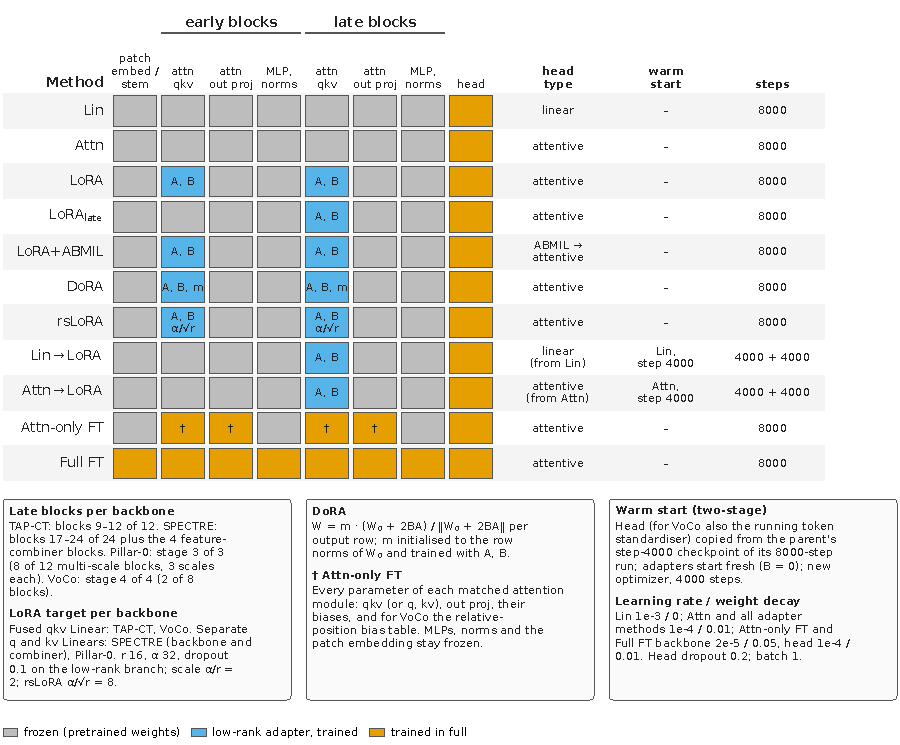
\includegraphics[width=\textwidth]{figures/fig_methods_cls.pdf}
\caption{Overview of the classification methods, drawn from the implementation: what each method trains inside every encoder block and the head (grey = frozen, blue = low-rank adapter, orange = trained in full), the head it uses, its warm start and its budget, with the late blocks and adapted projections per backbone. The data path of every backbone is drawn in Figure~\ref{fig:pipeline_cls} and the segmentation methods in Figure~\ref{fig:methods_seg} (Appendix~\ref{app:details}).}
\label{fig:methods_cls}
\end{figure}

\paragraph{Backbones.} We adapt four publicly released pretrained 3-D CT encoders of three architectural families (Figure~\ref{fig:pipeline_cls} in Appendix~\ref{app:details}). \textbf{TAP-CT-B-3D} \citep{veenboer2025tapct}, pretrained by DINOv2-style self-supervision, is a plain 12-block ViT-B \citep{dosovitskiy2021vit} with $4\times8\times8$ voxel patches, a class (CLS) token and four register tokens \citep{darcet2024registers}, applied to windows of $12\times224\times224$ voxels at native slice spacing. \textbf{SPECTRE-Large} \citep{claessens2025spectre}, pretrained by self-distillation and vision--language alignment with radiology reports, is a plain 24-block ViT-L with $16\times16\times8$ patches on crops of $128\times128\times64$ voxels at $0.5\times0.5\times1$\,mm, followed by a pretrained four-block feature combiner that attends over the crops of a volume. \textbf{Pillar-0} \citep{agrawal2025pillar0}, pretrained on CT and breast MRI of one academic centre, is used through its released head-CT encoder, a convolutional stem followed by three stages of multi-scale window-attention blocks that encode a whole $128\times256\times256$ volume from eleven intensity windows in one pass; its pretraining on head CT restricts it to the hemorrhage cohort. \textbf{VoCo-L} \citep{wu2024voco,wu2024vocolarge} is the encoder of a SwinUNETR-v2 \citep{hatamizadeh2022swinunetr,he2023swinunetrv2}, a four-stage Swin transformer \citep{liu2021swin} with patch merging between stages and no class token, applied to $96^3$ windows at 1.5\,mm; we use the released self-supervised checkpoint. Volumes are reoriented, resampled and intensity-normalised as in each backbone's pretraining (Appendix~\ref{app:details}).

\paragraph{Classification heads and methods.} Every backbone exposes a set of tokens per volume: the CLS token of every window (TAP-CT), the combiner tokens of the crops (SPECTRE), the multi-scale tokens of the whole volume (Pillar-0), or one token per window formed by the spatial means of the outputs of stages 2--4 (VoCo, 2688-dimensional). \textbf{Lin} reads a pooled feature (the mean window token, the combiner's CLS token or Pillar-0's pooled embedding) through dropout and one linear layer. \textbf{Attn} is an attentive probe \citep{bardes2024vjepa,chen2024cae}: a learnable CLS token joins the token set, two self-attention blocks run over it, and the CLS output is read out. The \numClsMethodsN{} methods differ only in what is trained inside the encoder (Figure~\ref{fig:methods_cls}): the \emph{frozen probes} Lin and Attn; \textbf{LoRA} \citep{hu2022lora} on the query, key and value projections of every block (rank 16, $\alpha=32$, dropout 0.1) and its variants \textbf{LoRA$_{\text{late}}$} (the last third of the blocks of TAP-CT and SPECTRE, the last stage of Pillar-0 and VoCo), \textbf{LoRA+ABMIL} (tokens pooled by gated attention \citep{ilse2018abmil} before the head), \textbf{DoRA} \citep{liu2024dora} and \textbf{rsLoRA} \citep{kalajdzievski2023rslora} (update scaled by $\alpha/\sqrt{r}$, four times the LoRA scale); the \emph{two-stage schedules} \textbf{Lin$\to$LoRA} and \textbf{Attn$\to$LoRA}, which train the probe for half the budget and warm-start late-block LoRA from it, in the spirit of probing before fine-tuning \citep{kumar2022lpft}; and \textbf{Attn-only FT}, which trains every parameter of the attention modules \citep{touvron2022three}, and \textbf{Full FT}, which trains every parameter. All adapted and fine-tuned models use the attentive head; Lin$\to$LoRA keeps the linear head of its parent.

\paragraph{Segmentation heads and methods.} The encoder yields a grid of tokens per crop from four depths: TAP-CT blocks 3, 6, 9 and 12 (one token per $4\times8\times8$ voxels), SPECTRE blocks 6, 12, 18 and 24 (per $8\times16\times16$ voxels) and the outputs of VoCo's four stages (strides 4 to 32). \textbf{Lin} is a $1\times1\times1$ convolution on the deepest grid, upsampled trilinearly. \textbf{Dec} is a light multi-depth decoder in the spirit of UNETR \citep{hatamizadeh2022unetr}: the four grids are projected, concatenated, fused by a $3^3$ convolution and upsampled to the voxel grid in stages (about 2.5\,M parameters, no skip connections from the input; Figure~\ref{fig:pipeline_seg}). \textbf{LoRA}, \textbf{LoRA$_{\text{late}}$} and \textbf{DoRA} add the adapters of classification under the Dec head, \textbf{Full FT} trains the encoder with it, and \textbf{Dec$\to$LoRA} trains Dec for half the budget and warm-starts all-block LoRA from it (Figure~\ref{fig:methods_seg}). Predictions are independent sigmoids per structure.

\paragraph{Per-task and joint training.} Every cohort and dataset is trained in two modes with the same data and selection rule (Figure~\ref{fig:modes}): \emph{per-task}, one model per label or structure, and \emph{joint}, one shared model with one output per label or structure. A \emph{label--mode pair} denotes one label (or structure) on one backbone in one mode. The joint classification loss sums over the labels known for a case, so a label weighs the same in both modes; the joint segmentation loss averages Dice and cross-entropy over structures. A joint model trains for the budget of one per-task model, so it uses $1/K$ of the steps of the $K$ per-task models it replaces, except where stated below.


\section{Experimental setup}
\label{sec:setup}
\paragraph{Data.} Classification uses five public CT cohorts with \numLabelsN{} binary labels (Table~\ref{tab:cohorts}): the CVPR26 cohort of the CVPR 2026 3-D CT foundation-model challenge, which groups AMOS \citep{ji2022amos} with 15 disease labels, COVID-CTset \citep{rahimzadeh2021covidctset} and LUNA25 nodule malignancy \citep{peeters2026luna25}; FDG-PET/CT \citep{gatidis2022fdgpetct}, whose four mutually exclusive diagnosis groups we predict from the CT alone as one-vs-rest labels; RSNA 2022 cervical-spine fractures \citep{lin2023rsnacsfdata} (patient level and C1--C7); RSNA 2023 abdominal trauma \citep{rudie2024ratic} (any injury and kidney, liver and spleen injury); and RSNA 2019 intracranial hemorrhage \citep{flanders2020rsnaich} (any hemorrhage and five subtypes). Segmentation uses AMOS22 (15 organs; \citealp{ji2022amos}), KiTS23\footnote{\url{https://github.com/neheller/kits23}} (kidney, tumor, cyst; \citealp{heller2023kits21}), LiTS (liver, tumor; \citealp{bilic2023lits}), MSD Pancreas (pancreas, tumor; \citealp{antonelli2022msd}) and TotalSegmentator \citep{wasserthal2023totalsegmentator,wasserthal2026totalsegdata}, whose 117 structures we merge within anatomical systems into 15 (Appendix~\ref{app:data}); \numStructuresN{} structures in all. Every source is divided into a training, a selection and a held-out split: for the CVPR26 cohort and AMOS22 the official validation cases are divided in halves, for the other sources the splits are fixed seeded divisions of the released labelled cases, with the official TotalSegmentator test split held out. Patients do not span splits where patient identifiers exist (FDG-PET/CT, RSNA 2023, RSNA 2019); the other sources are split per case. Pillar-0 is run on the hemorrhage cohort, and VoCo on FDG-PET/CT, RSNA 2022 and RSNA 2023 and on all segmentation datasets.

\paragraph{Training.} Every run uses AdamW with a linear warm-up over the first 10\% of the steps, cosine decay to $10^{-6}$, bf16 mixed precision and seed 42. A classification run trains 8000 steps at batch size 1 on a masked, positive-weighted binary cross-entropy; a segmentation run trains 8000 steps of four crops on soft Dice plus binary cross-entropy per structure; two-stage methods split the budget into halves. The joint models of the two 15-structure datasets (AMOS22, TotalSegmentator) train 24\,000 steps, and the CVPR26 joint model is additionally trained for 26\,000 steps as a longer schedule reported in the appendix. Each method has one default learning rate and weight decay, set once before the sweep by the type of parameter it trains, from the largest rate for a head on frozen features ($10^{-3}$; $10^{-2}$ for the segmentation linear probe) through low-rank adapters ($10^{-4}$) to the smallest for encoder weights ($2\times10^{-5}$), and not tuned on our data for any backbone, cohort or method (Tables~\ref{tab:optim} and~\ref{tab:optimseg}). Every 1000 steps both the selection and the held-out split are evaluated; the checkpoint with the best selection macro AUROC or mean Dice is kept and its held-out metric is reported. TotalSegmentator per-structure models use Lin, Dec, LoRA and Full FT only. The joint models of Lin, LoRA, Attn-only FT and Full FT (classification) and of Dec, LoRA and Full FT (segmentation) were trained with two further seeds on TAP-CT, SPECTRE and Pillar-0 (\numSeedsclsRunsN{} and \numSeedssegRunsN{} runs). All settings are listed in Appendix~\ref{app:details}.

\paragraph{Evaluation and statistics.} Held-out AUROC per label and Dice per structure and case are the metrics \citep{maierhein2024metrics}. Per label--mode pair, methods are compared with DeLong's test on AUROC \citep{delong1988} and with a paired case bootstrap on Dice, with Benjamini--Hochberg correction \citep{benjamini1995fdr} within each family of comparisons at $\alpha=0.05$, and ranked within each pair that has every method. The main comparisons are summarised at label level: each label counts once with its per-task and joint differences averaged, and the 95\% interval of the mean comes from a percentile bootstrap over cohorts, labels within cohorts and held-out cases within labels (Appendix~\ref{app:stats}); because four or five cohorts per backbone make the cohort stage optimistic, we also report the number of cohorts with a positive mean difference. Pooled estimates use TAP-CT, SPECTRE and Pillar-0; VoCo, which ran three of the five classification cohorts, is reported per backbone. A method whose held-out probabilities barely vary between cases did not train: we flag it when the median standard deviation of its held-out probabilities over label--mode pairs is below 0.01, keep it in the per-cohort tables and leave it out of ranks and averages over methods.


\section{Results}
\label{sec:results}
\begin{table}[tb]
\centering
\caption{Label-level comparisons on the three main backbones: mean difference in held-out AUROC (classification) or Dice (segmentation), its 95\% interval over cohorts, labels and held-out cases, and the number of cohorts (datasets) with a positive mean difference. Each label counts once with its per-task and joint differences averaged, except in the two LoRA $-$ Dec sub-rows. LoRA $-$ Attn compares two methods with the same attentive head. Pooled estimates (``all'') use TAP-CT, SPECTRE and Pillar-0; VoCo is in Table~\ref{tab:keyvoco}. $^{\dagger}$ = did not train with the default setting (Section~\ref{sec:fullft}).}
\label{tab:key}
\adjustbox{max width=\textwidth}{\small\begin{tabular}{@{}lccccc@{}}
\toprule
Comparison & TAP-CT & SPECTRE & Pillar-0 & All & Cohorts $>0$ \\
\midrule
\multicolumn{6}{@{}l}{\textit{Classification (AUROC)}} \\
LoRA $-$ Lin & \mci{+0.032}{+0.007}{+0.053} & \mci{+0.037}{+0.009}{+0.075} & \mci{+0.033}{+0.021}{+0.044} & \mci{+0.034}{+0.017}{+0.052} & 9/10 \\
LoRA $-$ Attn & \mci{+0.022}{+0.006}{+0.042} & \mci{+0.033}{+0.003}{+0.078} & \mci{+0.034}{+0.021}{+0.052} & \mci{+0.027}{+0.012}{+0.048} & 10/10 \\
Attn-only FT $-$ LoRA & \mci{+0.019}{-0.001}{+0.054} & \mci{+0.002}{-0.037}{+0.026} & \mci{+0.001}{-0.002}{+0.004} & \mci{+0.011}{-0.007}{+0.029} & 7/10 \\
Full FT $-$ Lin & \mci{+0.022}{-0.061}{+0.068} & \mci{-0.117}{-0.195}{-0.059}$^{\dagger}$ & \mci{+0.004}{-0.013}{+0.021} & \mci{-0.038}{-0.103}{+0.019} & 5/10 \\
joint $-$ per-task & \mci{+0.012}{-0.014}{+0.038} & \mci{-0.003}{-0.044}{+0.051} & \mci{-0.008}{-0.013}{-0.001} & \mci{+0.004}{-0.021}{+0.030} & 6/10 \\
\addlinespace
\multicolumn{6}{@{}l}{\textit{Segmentation (Dice)}} \\
Dec $-$ Lin & \mci{+0.085}{+0.055}{+0.109} & \mci{+0.061}{+0.027}{+0.088} & -- & \mci{+0.073}{+0.049}{+0.092} & 10/10 \\
LoRA $-$ Dec & \mci{-0.005}{-0.021}{+0.024} & \mci{+0.023}{-0.018}{+0.076} & -- & \mci{+0.009}{-0.015}{+0.046} & 8/10 \\
LoRA $-$ Dec, per-task & \mci{-0.021}{-0.036}{+0.002} & \mci{+0.006}{-0.003}{+0.031} & -- & \mci{-0.007}{-0.022}{+0.009} & 7/10 \\
LoRA $-$ Dec, joint & \mci{+0.011}{-0.021}{+0.066} & \mci{+0.040}{-0.039}{+0.147} & -- & \mci{+0.026}{-0.021}{+0.093} & 8/10 \\
Full FT $-$ Dec & \mci{0.000}{-0.024}{+0.016} & \mci{-0.003}{-0.035}{+0.009} & -- & \mci{-0.002}{-0.018}{+0.009} & 6/10 \\
joint $-$ per-task & \mci{-0.046}{-0.090}{-0.008} & \mci{-0.058}{-0.093}{-0.009} & -- & \mci{-0.052}{-0.082}{-0.022} & 0/10 \\
\bottomrule
\end{tabular}
}
\end{table}

We report held-out results of \numRunsMainN{} main runs and \numRunsRevisionN{} repeats and controls. Table~\ref{tab:key} summarises the main comparisons (per backbone in Figure~\ref{fig:key}, Appendix~\ref{app:perlabel}); per-cohort tables, ranks, per-label results and every paired test are in Appendix~\ref{app:perlabel}. The selection-split metric recomputed from the stored per-case predictions matched the value logged during training for every run (classification to $10^{-7}$; segmentation within $2\times10^{-3}$ for all but one of the \numSelcheckSegRunsN{} runs, whose per-case Dice was re-inferred after training).

\subsection{Classification}
\label{sec:cls}

\paragraph{Adapting the encoder improves on the frozen probes.} LoRA raises held-out AUROC over the linear probe by $\numCiClsloralinAllMeandiff$ at label level (95\% interval $\numCiClsloralinAllLodiff$ to $\numCiClsloralinAllHidiff$; positive in \numCiClsloralinAllPosN{} of \numCiClsloralinAllClustersN{} cohort--backbone pairs), with intervals above zero on each backbone: $\numCiClsloralinTapctMeandiff$ on TAP-CT, $\numCiClsloralinSpectreMeandiff$ on SPECTRE and $\numCiClsloralinPillarZMeandiff$ on Pillar-0. LoRA also changes the head, from linear to attentive, but the frozen attentive probe alone adds only $\numCiClsattnlinAllMeandiff$ ($\numCiClsattnlinAllLodiff$ to $\numCiClsattnlinAllHidiff$), and against this matched-head baseline LoRA gains $\numCiClsloraattnAllMeandiff$ ($\numCiClsloraattnAllLodiff$ to $\numCiClsloraattnAllHidiff$; positive in \numCiClsloraattnAllPosN{} of \numCiClsloraattnAllClustersN{} cohort--backbone pairs), so the gain comes from adapting the encoder. Leaving out FDG-PET/CT and COVID-CTset, two sources in which we did not rule out shortcuts, leaves it unchanged ($\numCiClsloralinnoscAllMeandiff$, $\numCiClsloralinnoscAllLodiff$ to $\numCiClsloralinnoscAllHidiff$). Per label--mode pair, LoRA is never significantly behind the linear probe and significantly ahead in \numPairedTapctLinLoraSigbetter\%, \numPairedSpectreLinLoraSigbetter\% and \numPairedPillarZLinLoraSigbetter\% of the pairs on TAP-CT, SPECTRE and Pillar-0; significance follows the held-out size rather than the effect (mean gain $\numSigbysizeSmallMeandiff$ and \numSigbysizeSmallSig\% significant below 100 held-out cases, $\numSigbysizeLargeMeandiff$ and \numSigbysizeLargeSig\% above 400; Figure~\ref{fig:perlabel}). LoRA is ahead of the linear probe in \numSeedsclsLoraLinAllPosN{} of \numSeedsclsLoraLinAllPairsN{} cohort--seed pairs of the seed repeats, and the gain is largest where the probe is weakest ($\numGainbinLowMeandiff$ for labels whose probe reaches a selection AUROC of at most 0.6, $\numGainbinTopMeandiff$ above 0.8).

\paragraph{Training the attention weights in full has the best mean rank, but its gain over LoRA is uncertain.} At the default settings and over the \numRankSlotsN{} label--mode pairs, attention-only fine-tuning has the best mean rank (\numRankAttnftMean{}; LoRA \numRankLoraMean{}, LoRA+ABMIL \numRankBabmilMean{}, DoRA \numRankDoraMean{}, linear probe \numRankLinMean{}; Figure~\ref{fig:ranks}). Its label-level difference to LoRA is $\numCiClsattnftloraAllMeandiff$ ($\numCiClsattnftloraAllLodiff$ to $\numCiClsattnftloraAllHidiff$): $\numCiClsattnftloraTapctMeandiff$ on TAP-CT but $\numCiClsattnftloraSpectreMeandiff$ on SPECTRE and $\numCiClsattnftloraPillarZMeandiff$ on Pillar-0. The LoRA variants do not improve on LoRA: on the same pairs, LoRA$_{\text{late}}$ changes AUROC by $\numVsloraAllLoragMeandiff$, DoRA by $\numVsloraAllDoraMeandiff$, rsLoRA by $\numVsloraAllRsloraMeandiff$, LoRA+ABMIL by $\numVsloraAllBabmilMeandiff$, and the two-stage schedules by $\numVsloraAllLinThenLoragMeandiff$ (Lin$\to$LoRA) and $\numVsloraAllAttnThenLoragMeandiff$ (Attn$\to$LoRA). The rsLoRA deficit on TAP-CT is a learning-rate effect: at a quarter of the rate, which matches its update scale to LoRA, it gains $\numCtrlTapctRsloraLowlrRsloraMeandiff$ (Appendix~\ref{app:revision}).

\paragraph{Full fine-tuning did not train on SPECTRE with the default setting.}\label{sec:fullft} The held-out probabilities of SPECTRE Full FT barely vary between cases (median standard deviation \numSpreadSpectreFullft{}, against at least \numSpreadOthermin{} for every other method on the three backbones), and it loses $\numCiClsfullftlinSpectreMeandiff$ to the linear probe. On TAP-CT it changes AUROC by $\numCiClsfullftlinTapctMeandiff$ ($\numCiClsfullftlinTapctLodiff$ to $\numCiClsfullftlinTapctHidiff$), with one collapsed joint run (FDG-PET/CT, \numClsAurocFdgTapctJointFullft{}), and it is the least stable method across seeds (median between-seed change of the cohort mean \numSeedsclsFullftSdmedian{}, LoRA \numSeedsclsLoraSdmedian{}). Of three alternative settings, layer-wise learning-rate decay (0.75 per block) gave SPECTRE Full FT the highest selection AUROC (\numFixSpectreFullftLlrdVal{}, against \numFixSpectreFullftLowlrVal{} with a lower learning rate and \numFixSpectreFullftAccumVal{} with gradient accumulation and clipping, which trained on \numFixSpectreFullftAccumTrainedN{} of \numFixSpectreFullftAccumCohortsN{} cohorts); with it Full FT is ahead of LoRA by $\numFixselSpectreLoraMeandiff$ on SPECTRE and level with it on TAP-CT ($\numFixselTapctLoraMeandiff$; Table~\ref{tab:revisioncls}), a comparison that favours Full FT, since LoRA was not re-tuned.

\paragraph{One joint model per cohort is as accurate as one model per label.} Joint minus per-task AUROC is $\numCiClsjointAllMeandiff$ ($\numCiClsjointAllLodiff$ to $\numCiClsjointAllHidiff$), at $1/K$ of the training steps of the $K$ per-task models; the sign varies by cohort from $\numJointdeltaMin$ to $\numJointdeltaMax$ (Figure~\ref{fig:joint}), and on Pillar-0 the joint model is behind on average, with an interval below zero ($\numCiClsjointPillarZMeandiff$, $\numCiClsjointPillarZLodiff$ to $\numCiClsjointPillarZHidiff$), though not for every method (Table~\ref{tab:cls}).

\subsection{Segmentation}
\label{sec:seg}

\paragraph{A decoder on the frozen encoder gives most of the gain.} Replacing the linear probe by the frozen decoder raises Dice by $\numCiSegdeclinAllMeandiff$ ($\numCiSegdeclinAllLodiff$ to $\numCiSegdeclinAllHidiff$), on every dataset of both backbones and significantly on \numSegpairedTapctLinDecSigbetter\% (TAP-CT) and \numSegpairedSpectreLinDecSigbetter\% (SPECTRE) of the structure--mode pairs. That is all of LoRA's gain over the linear probe on TAP-CT ($\numSegdeltaTapctLinLoraMeandiff$) and most of it on SPECTRE ($\numSegdeltaSpectreLinLoraMeandiff$).

\paragraph{Adapting the encoder on top of the decoder changes Dice little on average.} LoRA changes Dice relative to the frozen decoder by $\numCiSegloradecAllMeandiff$ ($\numCiSegloradecAllLodiff$ to $\numCiSegloradecAllHidiff$; $\numCiSegloradecTapctMeandiff$ on TAP-CT, $\numCiSegloradecSpectreMeandiff$ on SPECTRE). The sign depends on mode and dataset (Figure~\ref{fig:perstructure}): the largest gain is the SPECTRE AMOS22 joint model, where the decoder (\numSegAmosBBSpectreJointDec{}) falls below the linear probe (\numSegAmosBBSpectreJointLin{}) and LoRA reaches \numSegAmosBBSpectreJointLora{}, while on the TotalSegmentator joint model LoRA loses on both backbones (\numSegTotalsegSpectreJointLora{} against \numSegTotalsegSpectreJointDec{} on SPECTRE). LoRA is significantly ahead of the decoder on \numSegpairedSpectreDecLoraSigbetter\% of SPECTRE pairs and behind on \numSegpairedSpectreDecLoraSigworse\%; on TAP-CT on \numSegpairedTapctDecLoraSigbetter\% and \numSegpairedTapctDecLoraSigworse\%. Full fine-tuning has the best mean rank (\numSegrankFullftMean{}; LoRA \numSegrankLoraMean{}, Dec \numSegrankDecMean{}), on the strength of TAP-CT, but its mean change relative to the decoder is $\numCiSegfullftdecAllMeandiff$ ($\numCiSegfullftdecAllLodiff$ to $\numCiSegfullftdecAllHidiff$) because \numSegdeltaTapctDecFullftDropN{} TAP-CT structure--mode pairs lose more than 0.1 Dice. DoRA, LoRA$_{\text{late}}$ and Dec$\to$LoRA change Dice relative to the decoder by $\numCiSegdoradecAllMeandiff$, $\numCiSegloragdecAllMeandiff$ and $\numCiSegdecthenloradecAllMeandiff$, each with an interval that includes zero.

\paragraph{One model per structure is more accurate than one joint model at our budgets.} One joint model per dataset changes Dice by $\numCiSegjointAllMeandiff$ ($\numCiSegjointAllLodiff$ to $\numCiSegjointAllHidiff$), on none of the \numCiSegjointAllClustersN{} dataset--backbone pairs positive, most on the 15-structure AMOS22 ($\numSegjointdsAmosBBTapctMeandiff$, $\numSegjointdsAmosBBSpectreMeandiff$) and least on LiTS ($\numSegjointdsLitsTapctMeandiff$, $\numSegjointdsLitsSpectreMeandiff$). Much of the cost comes from small structures the joint model loses entirely: in \numSegcollapseN{} of \numSegcollapseCellsN{} structure--method pairs, all on the adrenal glands and the esophagus of AMOS22 and the merged glands of TotalSegmentator, the joint model scores below 0.01 Dice where the per-structure model reaches \numSegcollapsePertaskminValue{} to \numSegcollapsePertaskmaxValue{}; without them the mean difference over structure--method pairs moves from $\numSegjointTapctMeandiff$ to $\numSegjointTapctNocollapseMeandiff$ on TAP-CT and from $\numSegjointSpectreMeandiff$ to $\numSegjointSpectreNocollapseMeandiff$ on SPECTRE. Tripling the steps of the 15-structure joint models gained $\numSegbudgetgainTapctMeandiff$ and $\numSegbudgetgainSpectreMeandiff$, and at matched total compute (per-structure models of 1600 steps) the joint model is ahead with LoRA ($\numCmAmosBBTapctLoraJointdiff$ to $\numCmAmosBBSpectreLoraJointdiff$ on AMOS22) but behind with the frozen decoder and full fine-tuning in three of the four dataset--backbone pairs (Table~\ref{tab:computematched}). The gain from tripling the steps shows that the segmentation budget was short; \numConvSegAllLateBetter\% of segmentation runs also selected one of their last two validations, against \numConvClsAllLateBetter\% in classification, a share that the cosine decay of the learning rate inflates and that therefore indicates rather than measures under-training. The segmentation comparisons rank methods under a fixed budget, not at convergence.

\subsection{A fourth backbone: the hierarchical VoCo encoder}
\label{sec:voco}

VoCo differs from the three main backbones in its token interface (no class token, one stage-pooled token per $96^3$ window) and ran three of the five classification cohorts (\numLabelsVocoN{} labels) with the settings of the other backbones, so we report it separately (Appendix~\ref{app:voco}). In segmentation the findings hold: the decoder adds $\numCiSegdeclinVocoMeandiff$ Dice to a linear probe on the stride-32 output that segments almost nothing, LoRA changes Dice relative to the decoder by $\numCiSegloradecVocoMeandiff$ ($\numCiSegloradecVocoLodiff$ to $\numCiSegloradecVocoHidiff$), one joint model costs $\numCiSegjointVocoMeandiff$, and full fine-tuning is ahead of the decoder by $\numCiSegfullftdecVocoMeandiff$ ($\numCiSegfullftdecVocoLodiff$ to $\numCiSegfullftdecVocoHidiff$). In classification the picture differs: LoRA changes AUROC relative to the linear probe by $\numCiClsloralinVocoMeandiff$ ($\numCiClsloralinVocoLodiff$ to $\numCiClsloralinVocoHidiff$), behind on all \numCiClsloralinVocoClustersN{} cohorts, but more than half of this deficit comes from the head: the frozen attentive probe is itself behind the linear probe ($\numCiClsattnlinVocoMeandiff$), and against this matched-head baseline every method that adapts the encoder is level, with intervals including zero (LoRA $\numCiClsloraattnVocoMeandiff$, attention-only fine-tuning $\numCiClsattnftattnVocoMeandiff$, full fine-tuning $\numCiClsfullftattnVocoMeandiff$; Figure~\ref{fig:voco}). The only adapted method level with the linear probe is Lin$\to$LoRA, which keeps the linear head ($\numCiClslinthenloraglinVocoMeandiff$, $\numCiClslinthenloraglinVocoLodiff$ to $\numCiClslinthenloraglinVocoHidiff$). On VoCo, adapting the encoder therefore did not improve on a frozen probe with the same head, unlike on the three main backbones, and the attentive head on VoCo's 2688-dimensional window tokens was worse than a linear one. One joint model is again level with per-task models ($\numCiClsjointVocoMeandiff$). VoCo was run with the settings of the other backbones; whether a learning rate, head or window token chosen for it would change this we did not test, so the result bounds the transfer of the classification finding at the default settings rather than explaining it.


\section{Discussion}
\label{sec:discussion}
\paragraph{A practical guide.} Each step gives the expected change and the strength of the evidence: \emph{consistent} (the label-level interval excludes zero with the same sign on TAP-CT and SPECTRE), \emph{conditional} (the sign depends on the backbone, mode or budget) or \emph{uncertain} (the interval includes zero).
\begin{enumerate}\setlength{\itemsep}{1pt}
  \item \textbf{Classification: adapt the attention weights.} Rank-16 LoRA on the query, key and value projections of every block, with an attentive head, adds $\numCiClsloralinAllMeandiff$ AUROC over the linear probe (\emph{consistent}); training the attention projections in full adds $\numCiClsattnftloraTapctMeandiff$ over LoRA on TAP-CT only (\emph{uncertain}). Compare against both frozen probes on selection data: on VoCo, with the same settings, adapting the encoder was level with the attentive probe and both were behind the linear probe (\emph{conditional} on the backbone). These are default settings; only full fine-tuning was re-tuned.
  \item \textbf{Classification: one joint model per cohort is a reasonable default.} It is level with per-task models on average ($\numCiClsjointAllMeandiff$) at one run instead of one per label, with a sign that varies by cohort (\emph{uncertain} for a given cohort).
  \item \textbf{Segmentation: put a multi-depth decoder on the frozen encoder, and adapt the encoder only if it helps on selection data.} The decoder adds $\numCiSegdeclinTapctMeandiff$ and $\numCiSegdeclinSpectreMeandiff$ Dice over a linear probe (\emph{consistent}); LoRA on top of it changed Dice by $\numCiSegloradecTapctMeandiff$ and $\numCiSegloradecSpectreMeandiff$ (\emph{conditional}).
  \item \textbf{Segmentation: train one model per structure when Dice matters most, or give a joint model more steps.} A joint model changed Dice by $\numCiSegjointTapctMeandiff$ and $\numCiSegjointSpectreMeandiff$ at our budgets (\emph{consistent}), and tripling its steps added $\numSegbudgetgainTapctMeandiff$ and $\numSegbudgetgainSpectreMeandiff$; at matched compute the sign depends on the method (\emph{conditional}).
  \item \textbf{Treat full fine-tuning and the LoRA variants as options to validate.} With the default setting full fine-tuning did not train SPECTRE, so check that predictions vary between cases; layer-wise learning-rate decay made it train. In segmentation it can lose a structure the decoder segments, so monitor per-structure selection Dice (\emph{conditional}). The LoRA variants were level with plain LoRA or below it (\emph{uncertain}).
\end{enumerate}

\paragraph{Limitations.} Each method has one default learning rate and budget, set without tuning, and only full fine-tuning was retrained with other settings after it failed; full fine-tuning and rsLoRA proved sensitive to the default, so the ranking among the stronger methods may change with tuning. Only the joint models of seven method--task pairs were repeated with further seeds. Segmentation had not converged, and its results rank adaptation methods under one budget rather than measure how close these models come to task-specific networks; Dice is computed on each backbone's working grid without post-processing. SPECTRE's pretraining images include several of our evaluation sets, which affects comparisons between backbones (Appendix~\ref{app:perlabel}). Pillar-0 enters through one cohort and VoCo through three. For most sources the splits are our own seeded divisions of the released labelled cases; we release them with the per-case predictions. One author co-developed TAP-CT; all backbones use the same protocol and settings.

\paragraph{Conclusion.} Adapting the attention weights of a pretrained 3-D CT encoder improves classification over both frozen probes on TAP-CT, SPECTRE and Pillar-0, and one joint model per cohort is as accurate as one model per label; on the hierarchical VoCo encoder, at the same default settings, adapting the encoder was level with the matched frozen probe. For segmentation, a multi-depth decoder on the frozen encoder gives most of the gain, adapting the encoder on top of it changes Dice little on average, and one model per structure is more accurate than one joint model at our budgets. Code, splits and per-case predictions are released at \todo{public repository URL}.


\clearpage
\bibliography{refs}

\appendix
\section{Data}
\label{app:data}

\begin{table}[htbp]
\centering
\caption{Cohorts and datasets. Labels = binary labels (classification) or structures (segmentation); counts are cases in the training / selection / held-out splits as read from the manifests. Split rule: ``official val, halves'' = the official validation cases sorted by identifier and alternately assigned to the selection and held-out split; ``seeded'' = one fixed seeded division of the released labelled cases (80/10/10 of the released training data for the three RSNA and FDG cohorts, 70/15/15 for KiTS23 and MSD Pancreas, 91/20/20 volumes for LiTS); TotalSegmentator holds out its official test split and takes an equally large selection split from the official training split. FDG-PET/CT cases are studies (1014 studies of 900 patients; no patient spans splits); RSNA 2019 training cases are a stratified subset of the released training patients. Backbones: T = TAP-CT, S = SPECTRE, P = Pillar-0, V = VoCo.}
\label{tab:cohorts}
\adjustbox{max width=\textwidth}{\small
\begin{tabular}{@{}llllrrr@{}}
\toprule
Cohort / dataset & Labels & Split rule & Backbones & Train & Sel. & Held-out \\
\midrule
\multicolumn{7}{@{}l}{\textit{Classification}} \\
CVPR26: AMOS & 15 disease labels & official val, halves & T S & 1463$^\dagger$ & \numCasesCvprAmosVal & \numCasesCvprAmosTest \\
CVPR26: COVID-CTset & COVID-19 & official val, halves & T S & 308 & \numCasesCvprCovidVal & \numCasesCvprCovidTest \\
CVPR26: LUNA25 & nodule malignancy & official val, halves & T S & 1000 & \numCasesCvprLunaVal & \numCasesCvprLunaTest \\
FDG-PET/CT & 4 diagnosis groups & seeded, patient level & T S V & 776 & 116 & 122 \\
RSNA 2022 C-spine & patient, C1--C7 (8) & seeded, per study & T S V & 1615 & 202 & 202 \\
RSNA 2023 trauma & any, kidney, liver, spleen (4) & seeded, one series per patient & T S V & 2517 & 315 & 315 \\
RSNA 2019 hemorrhage & any + 5 subtypes (6) & stratified, patient level & T S P & 5000 & 3269 & 3264 \\
\addlinespace[2pt]
\multicolumn{7}{@{}l}{\textit{Segmentation}} \\
AMOS22 & 15 organs & official val, halves & T S V & 200 & 50 & 50 \\
KiTS23 & kidney, tumor, cyst & seeded & T S V & 343 & 73 & 73 \\
LiTS & liver, tumor & seeded & T S V & 91 & 20 & 20 \\
MSD Pancreas & pancreas, tumor & seeded & T S V & 197 & 42 & 42 \\
TotalSegmentator & 15 merged structures & official test held out & T S V & 1721 & 109 & 109 \\
\bottomrule
\end{tabular}}
\\[2pt]{\footnotesize $^\dagger$ distinct AMOS cases over the 15 per-label files; each label is known for a subset of cases.}
\end{table}

\begin{table}[htbp]
\centering
\caption{TotalSegmentator: the 117 released structures merged into 15 within anatomical systems, as implemented. Where two source masks overlap, the voxel is assigned to the smaller structure.}
\label{tab:totalseg}
\small
\begin{tabular}{@{}lp{0.72\textwidth}@{}}
\toprule
Structure & Source structures \\
\midrule
lungs and airway & five lung lobes, trachea \\
heart & heart, left atrial appendage \\
arteries & aorta, brachiocephalic trunk, left and right subclavian, common carotid and iliac arteries \\
veins & superior and inferior vena cava, left and right brachiocephalic and iliac veins, portal and splenic vein, pulmonary vein \\
liver & liver, gallbladder \\
spleen & spleen \\
pancreas & pancreas \\
kidneys & left and right kidney, left and right kidney cysts \\
GI tract & esophagus, stomach, duodenum, small bowel, colon \\
bladder and prostate & urinary bladder, prostate \\
glands & thyroid, left and right adrenal gland \\
brain and spinal cord & brain, spinal cord \\
spine & 25 vertebrae (C1--L6), sacrum \\
other bones & 24 ribs, sternum, costal cartilages, clavicles, scapulae, humeri, hip bones, femurs, skull \\
muscles & gluteus maximus, medius and minimus, iliopsoas, autochthon (left and right) \\
\bottomrule
\end{tabular}
\end{table}

\section{Training and evaluation details}
\label{app:details}

\begin{figure}[htbp]
\centering
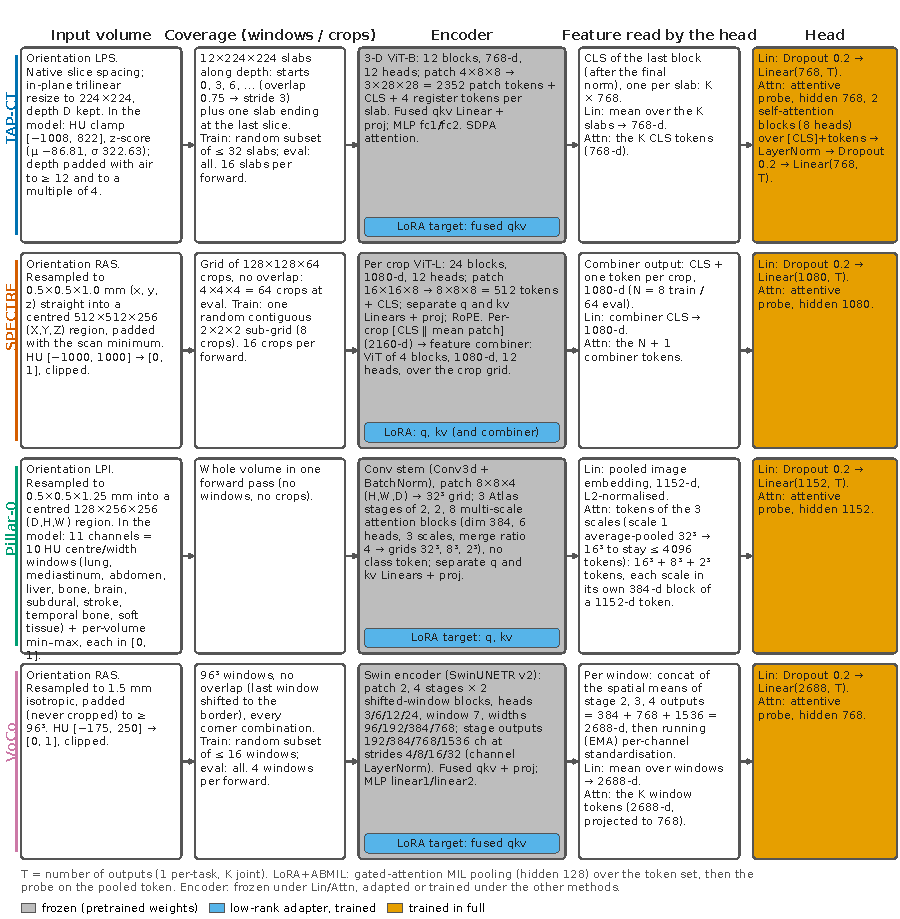
\includegraphics[width=\textwidth]{figures/fig_pipeline_cls.pdf}
\caption{Overview of the classification path, drawn from the implementation. Each row is one backbone: the volume is resampled and windowed as in pretraining, covered by windows or crops, encoded, and reduced to the feature the head reads. Lin reads one pooled feature per volume, Attn the set of window, crop or scale tokens. Grey = frozen, blue = low-rank adapter, orange = trained in full.}
\label{fig:pipeline_cls}
\end{figure}

\begin{figure}[htbp]
\centering
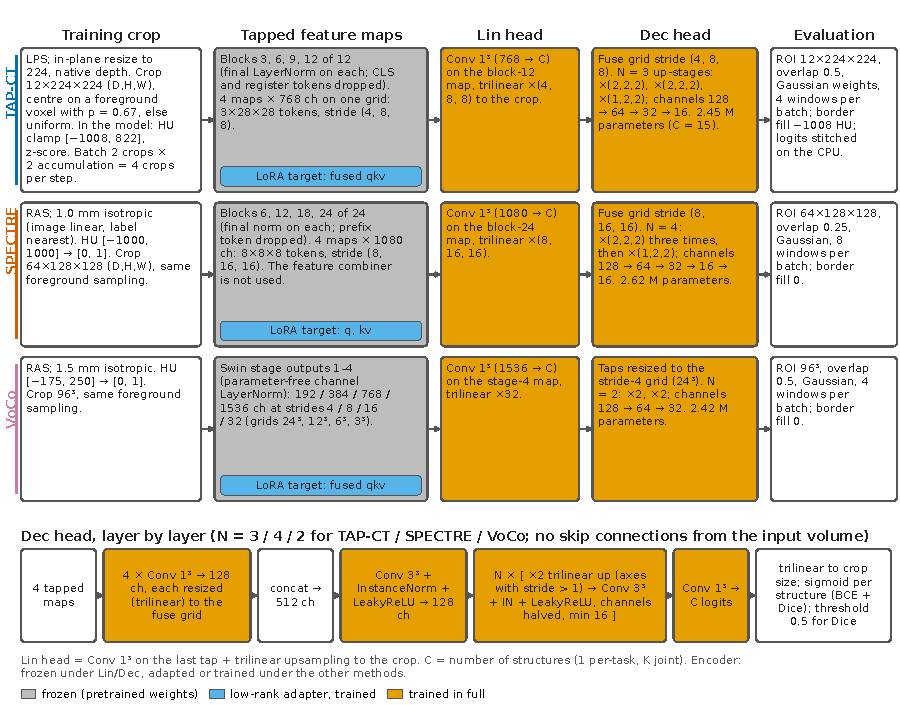
\includegraphics[width=\textwidth]{figures/fig_pipeline_seg.pdf}
\caption{Overview of the segmentation path, drawn from the implementation: crop geometry per backbone, the four tapped depths with their strides and channels, the linear probe on the deepest grid, and the multi-depth decoder layer by layer. Grey = frozen, blue = low-rank adapter, orange = trained in full.}
\label{fig:pipeline_seg}
\end{figure}

\begin{figure}[htbp]
\centering
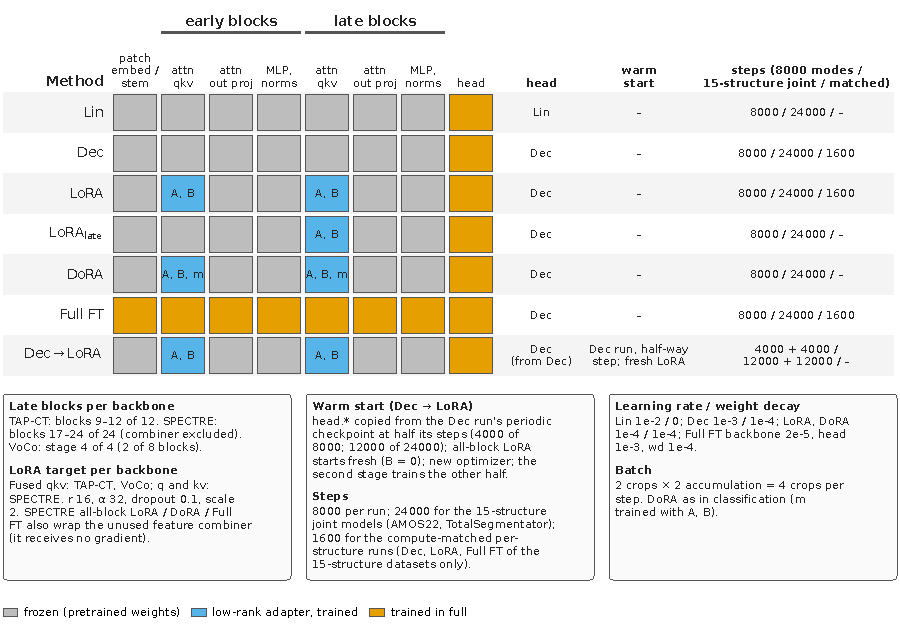
\includegraphics[width=\textwidth]{figures/fig_methods_seg.pdf}
\caption{What each segmentation method trains, the head it uses, its warm start and its budget.}
\label{fig:methods_seg}
\end{figure}

\begin{figure}[htbp]
\centering
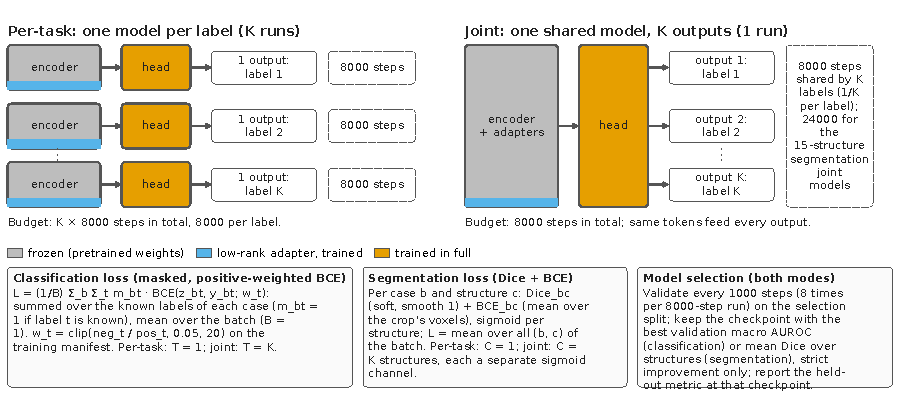
\includegraphics[width=\textwidth]{figures/fig_modes.pdf}
\caption{Per-task and joint training, the two losses, the step budgets and the selection rule.}
\label{fig:modes}
\end{figure}

\paragraph{Input preprocessing.} Every volume is reoriented to the frame of the backbone's pretraining and resampled to its grid. TAP-CT: LPS, native slice spacing, in-plane trilinear resize to $224\times224$, depth padded with air to at least 12 slices and to a multiple of 4; HU clipped to $[-1008, 822]$ and standardised with the model's mean and standard deviation; windows of 12 slices with a stride of 3 slices plus a final window ending at the last slice (at most 32 windows per training step, all windows at evaluation). SPECTRE: RAS, $0.5\times0.5\times1$\,mm, centred $512\times512\times256$ field of view padded with the scan minimum, HU in $[-1000, 1000]$ scaled to $[0,1]$; a $4\times4\times4$ grid of 64 crops of $128\times128\times64$ voxels at evaluation and a random contiguous $2\times2\times2$ sub-grid of 8 crops at training; each crop is summarised by its CLS token concatenated with its mean patch token before the feature combiner. Pillar-0: LPI, $0.5\times0.5\times1.25$\,mm, centred $128\times256\times256$ volume, eleven input channels (ten fixed centre/width windows and a per-volume min--max channel), one forward pass; the linear head reads the model's L2-normalised pooled embedding (three scales concatenated, 1152-d), the attentive head reads the tokens of the three scales, any scale with more than 4096 tokens being average-pooled on its grid. VoCo: RAS, 1.5\,mm isotropic, HU in $[-175, 250]$ scaled to $[0,1]$, padded to at least $96^3$ and covered by non-overlapping $96^3$ windows (the last window shifted to the border; at most 16 windows per training step); each window becomes one 2688-dimensional token, the concatenation of the spatial means of the stage-2, 3 and 4 outputs, standardised per channel with running statistics (momentum 0.01) that are stored with the checkpoint. For segmentation, TAP-CT keeps the classification grid (in-plane 224, native depth) and crops of $12\times224\times224$ voxels; SPECTRE resamples to 1\,mm and uses crops of $64\times128\times128$ voxels; VoCo resamples to 1.5\,mm and uses $96^3$ crops. A training crop is centred on a random foreground voxel of the run's structures with probability 0.67 and placed uniformly otherwise; volumes smaller than the crop are padded with the image minimum. At evaluation the whole volume is covered by a sliding window with Gaussian weighting (overlap 0.5 for TAP-CT and VoCo, 0.25 for SPECTRE) and Dice is computed on the backbone's working grid, without post-processing.

\paragraph{Heads.} The linear head is dropout (0.2) followed by one linear layer on the pooled feature: the mean of the window CLS tokens for TAP-CT (768-d), the feature combiner's CLS token for SPECTRE (1080-d), the pooled image embedding for Pillar-0 (1152-d) and the mean window token for VoCo (2688-d). The attentive probe prepends a learnable CLS token to the token set (the window CLS tokens for TAP-CT, the combiner tokens for SPECTRE, the multi-scale tokens for Pillar-0, the window tokens for VoCo; VoCo's tokens are first projected from 2688 to 768 dimensions), applies two pre-norm transformer blocks with eight-head self-attention and a GELU feed-forward layer of ratio 4, normalises the CLS output and maps it through dropout (0.2) and a linear layer. LoRA+ABMIL pools the window or crop tokens by gated attention \citep{ilse2018abmil}, $a_i=\mathrm{softmax}_i\big(\bm{w}^\top(\tanh(\bm{V}\bm{x}_i)\odot\sigma(\bm{U}\bm{x}_i))\big)$ with hidden size 128, and feeds the pooled token to the attentive probe. The segmentation linear probe is a $1\times1\times1$ convolution on the deepest grid (TAP-CT block 12, SPECTRE block 24, VoCo stage 4 at stride 32), upsampled trilinearly. The decoder projects each of the four grids to 128 channels with a $1\times1\times1$ convolution, resizes them to a common grid (the token grid for the two ViTs, the stride-4 grid for VoCo), concatenates them (512 channels), fuses them with a $3^3$ convolution, instance normalisation and leaky ReLU to 128 channels, then applies stages of trilinear $\times2$ upsampling followed by the same convolution block that halves the channels (to a minimum of 16) until the voxel grid is reached (three stages for TAP-CT, four for SPECTRE, two for VoCo), and ends with a $1\times1\times1$ convolution to one logit per structure. It has 2.45\,M (TAP-CT), 2.62\,M (SPECTRE) and 2.42\,M (VoCo) parameters plus $17C$ or $33C$ for $C$ structures, and no skip connections from the input.

\paragraph{Adapters.} LoRA \citep{hu2022lora} replaces a frozen projection $\bm{W}_0\bm{x}$ by $\bm{W}_0\bm{x}+\tfrac{\alpha}{r}\bm{B}\bm{A}\,\mathrm{drop}(\bm{x})$ with $r=16$, $\alpha=32$ and dropout 0.1; $\bm{A}$ is initialised Kaiming-uniform and $\bm{B}$ at zero, so training starts from the pretrained model. It is applied to the fused query/key/value projection of every TAP-CT and VoCo block and to the separate query and key/value projections of every SPECTRE block, of SPECTRE's feature combiner, and of every Pillar-0 block. Late adapters cover TAP-CT blocks 9--12, SPECTRE blocks 17--24 and its feature combiner, the third stage of Pillar-0 (8 of 12 blocks) and the fourth stage of VoCo (2 of 8 blocks). rsLoRA scales the update by $\alpha/\sqrt{r}$ instead of $\alpha/r$. DoRA \citep{liu2024dora} rescales each row of the adapted weight to a learned magnitude $\bm{m}$, $\bm{W}=\bm{m}\odot(\bm{W}_0+\tfrac{\alpha}{r}\bm{B}\bm{A})/\lVert\bm{W}_0+\tfrac{\alpha}{r}\bm{B}\bm{A}\rVert_{\text{row}}$, with $\bm{m}$ initialised to the row norms of $\bm{W}_0$; the magnitude is a two-dimensional parameter and receives weight decay like the adapter matrices. Attention-only fine-tuning unfreezes every parameter of the attention modules that LoRA would adapt (query, key, value and output projections with their biases, and for VoCo the relative position bias). In segmentation the SPECTRE adapters and full fine-tuning also cover the feature combiner, which the segmentation path does not evaluate; those parameters receive no gradient.

\paragraph{Two-stage methods.} Lin$\to$LoRA and Attn$\to$LoRA take the probe weights (for VoCo also the running standardisation statistics of the window tokens) from the parent run's checkpoint at step 4000 of its 8000-step schedule, add late-block LoRA with $\bm{B}=0$, and train 4000 further steps with a fresh optimiser and schedule. Dec$\to$LoRA takes the decoder from the Dec run at the midpoint of its schedule (step 4000; step 12\,000 for the 24\,000-step joint models) and trains all-block LoRA with the decoder for the second half.

\paragraph{Optimisation.} AdamW uses $\beta=(0.9, 0.999)$ and $\epsilon=10^{-8}$ (the framework defaults; no run overrides them). The learning rate rises linearly from 1\% of its peak over the first 10\% of the steps and then follows a cosine to $10^{-6}$. Weight decay is applied to parameters of dimension two or more, excluding biases and normalisation weights. Gradients are not clipped. Classification trains at batch size 1 without gradient accumulation; segmentation at a micro-batch of 2 crops with accumulation 2, so four crops per step. The classification loss for a case with logits $\bm{z}$, labels $\bm{y}$ and known-label mask $\bm{m}$ is
\begin{equation}
\mathcal{L}_{\text{cls}}=\frac{1}{B}\sum_{b=1}^{B}\sum_{t} m_{bt}\,\mathrm{BCE}(z_{bt}, y_{bt}; w_t), \qquad w_t=\mathrm{clip}\Big(\frac{n^{-}_t}{n^{+}_t}, 0.05, 20\Big),
\label{eq:lcls}
\end{equation}
where $\mathrm{BCE}(\cdot;w_t)$ is the binary cross-entropy with positive weight $w_t$ computed from the negative and positive counts of label $t$ in the training split. The segmentation loss per case $b$ and structure $c$, with $\bm{p}=\sigma(\bm{z})$ over the $V$ voxels of a crop and reference $\bm{y}$, is
\begin{equation}
\mathcal{L}_{\text{seg}}=\frac{1}{BC}\sum_{b,c}\Big[1-\frac{2\sum_v p_{bcv}y_{bcv}+1}{\sum_v p_{bcv}+\sum_v y_{bcv}+1}+\frac{1}{V}\sum_v \mathrm{BCE}(z_{bcv},y_{bcv})\Big].
\label{eq:lseg}
\end{equation}
In the joint CVPR26 models the three sources are sampled in the ratio 10:8:8 (AMOS, COVID-CTset, LUNA25); every other run cycles one shuffled training set.

\begin{table}[htbp]
\centering
\caption{Classification settings per method. LoRA-type adapters have rank 16, $\alpha=32$ and dropout 0.1. Learning rate and weight decay apply to every trained parameter unless a backbone/head pair is given. All runs: AdamW, 8000 steps (two-stage: 4000 + 4000), batch size 1, warm-up 10\%, cosine to $10^{-6}$, bf16, head dropout 0.2.}
\label{tab:optim}
\adjustbox{max width=\textwidth}{\small
\begin{tabular}{@{}llll@{}}
\toprule
Method & Trained in the encoder & Head & Learning rate / weight decay \\
\midrule
Lin & nothing & linear & $10^{-3}$ / 0 \\
Attn & nothing & attentive & $10^{-4}$ / 0.01 \\
LoRA & LoRA on q, k, v of every block & attentive & $10^{-4}$ / 0.01 \\
LoRA$_{\text{late}}$ & LoRA on q, k, v of the late blocks & attentive & $10^{-4}$ / 0.01 \\
LoRA+ABMIL & as LoRA & ABMIL then attentive & $10^{-4}$ / 0.01 \\
DoRA & DoRA on q, k, v of every block & attentive & $10^{-4}$ / 0.01 \\
rsLoRA & LoRA, scale $\alpha/\sqrt{r}$ & attentive & $10^{-4}$ / 0.01 \\
Lin$\to$LoRA & late LoRA from step 4000 of Lin & linear (inherited) & $10^{-4}$ / 0.01 \\
Attn$\to$LoRA & late LoRA from step 4000 of Attn & attentive (inherited) & $10^{-4}$ / 0.01 \\
Attn-only FT & all attention parameters & attentive & encoder $2\times10^{-5}$ / 0.05, head $10^{-4}$ / 0.01 \\
Full FT & every parameter & attentive & encoder $2\times10^{-5}$ / 0.05, head $10^{-4}$ / 0.01 \\
\midrule
\multicolumn{4}{@{}l}{\textit{Repeats and controls (Appendix~\ref{app:revision})}} \\
Full FT, lower LR & every parameter & attentive & encoder $5\times10^{-6}$ / 0.05, head $10^{-4}$ / 0.01 \\
Full FT, layer decay & every parameter, LR $\times0.75$ per block from the top & attentive & encoder $2\times10^{-5}$ / 0.05, head $10^{-4}$ / 0.01 \\
Full FT, accumulation & every parameter; accumulation 8, clipping 1.0, 1000 steps & attentive & as Full FT \\
MLP-only FT & both MLP layers of every block & attentive & encoder $2\times10^{-5}$ / 0.05, head $10^{-4}$ / 0.01 \\
rsLoRA, matched LR & LoRA, scale $\alpha/\sqrt{r}$ & attentive & $2.5\times10^{-5}$ / 0.01 \\
\bottomrule
\end{tabular}}
\end{table}

\begin{table}[htbp]
\centering
\caption{Segmentation settings per method. All runs: AdamW, 8000 steps (24\,000 for the AMOS22 and TotalSegmentator joint models; two-stage methods split the budget in halves), four crops per step, warm-up 10\%, cosine to $10^{-6}$, bf16. LoRA-type adapters as in Table~\ref{tab:optim}.}
\label{tab:optimseg}
\adjustbox{max width=\textwidth}{\small
\begin{tabular}{@{}llll@{}}
\toprule
Method & Trained in the encoder & Head & Learning rate / weight decay \\
\midrule
Lin & nothing & linear probe & $10^{-2}$ / 0 \\
Dec & nothing & decoder & $10^{-3}$ / $10^{-4}$ \\
LoRA & LoRA on q, k, v of every block & decoder & $10^{-4}$ / $10^{-4}$ \\
LoRA$_{\text{late}}$ & LoRA on q, k, v of the late blocks & decoder & $10^{-4}$ / $10^{-4}$ \\
DoRA & DoRA on q, k, v of every block & decoder & $10^{-4}$ / $10^{-4}$ \\
Full FT & every parameter & decoder & encoder $2\times10^{-5}$, head $10^{-3}$ / $10^{-4}$ \\
Dec$\to$LoRA & all-block LoRA from the midpoint of Dec & decoder (inherited) & $10^{-4}$ / $10^{-4}$ \\
\midrule
\multicolumn{4}{@{}l}{\textit{Controls (Appendix~\ref{app:revision})}} \\
From scratch & every parameter, encoder re-initialised & decoder & as Full FT \\
Compute-matched per-structure & Dec, LoRA, Full FT at 1600 steps per structure & decoder & as above \\
\bottomrule
\end{tabular}}
\end{table}

\paragraph{Model selection and per-case outputs.} Every 1000 steps the selection and held-out splits are evaluated and a checkpoint of the trained parameters is written; the checkpoint with the highest selection macro AUROC (mean over labels with both classes present) or mean Dice (mean over structures of the mean over cases in which the structure is present in the reference or the prediction) is kept, ties keeping the earlier checkpoint. For TotalSegmentator only the selection split is evaluated during training; the held-out split is evaluated afterwards with the selected checkpoint, and the recomputed selection Dice is required to match the recorded value within 0.005. Per case, the held-out probability of every known label (classification) and the Dice of every structure (segmentation) at the selected checkpoint are stored and are the input of every number in this paper. Dice thresholds the logits at 0; a structure enters a case's mean when the reference or the prediction contains it, so a false-positive structure scores 0 and an absent, unpredicted structure is skipped.

\section{Statistical procedure}
\label{app:stats}
Every number in this paper is computed by one script from the stored per-case predictions of the selected checkpoint of every run (\numRunsAllN{} runs; the classification files hold the held-out probability of every known label of every case, the segmentation files the Dice of every structure of every case).

\paragraph{Per-run metrics.} AUROC is the Mann--Whitney statistic with midranks (tied scores count one half); a label is skipped for a run when its selection or held-out split has fewer than two cases or a single class, which did not occur. Dice per structure is the mean over the held-out cases in which the structure is present in the reference or the prediction; an absent, unpredicted structure is skipped and a false-positive structure counts as 0. Cohort and dataset means (Tables~\ref{tab:cls} and~\ref{tab:seg}) are means over the labels or structures of complete cells. The recomputed selection-split macro metric was compared with the value logged during training for every run: all \numSelcheckClsRunsN{} classification runs agree to $10^{-7}$, and all but one of the \numSelcheckSegRunsN{} segmentation runs within $2\times10^{-3}$ (\numSegrecompRunsN{} segmentation runs had their per-case Dice re-inferred from the selected checkpoint after training; the one exception differs by $2.01\times10^{-3}$).

\paragraph{Did-not-train rule.} For each backbone and method, the median over label--mode pairs of the standard deviation of the held-out probabilities is computed; a median below \numSpreadMinValue{} flags a method that did not train. Only SPECTRE Full FT is flagged (\numSpreadSpectreFullft{}; every other method on TAP-CT, SPECTRE and Pillar-0 is at least \numSpreadOthermin{}). It stays in the per-cohort tables, the paired tests and the Full FT $-$ Lin estimate, and leaves the ranks and every average over methods. VoCo spreads are reported (Table~\ref{tab:spread}) but the rule is not applied to VoCo, whose methods have small spreads at held-out AUROCs well above chance.

\paragraph{Paired tests.} Per backbone, cohort, mode (per-task, joint) and label, every method is compared with the baselines Lin, LoRA, Attn and Full FT (classification; two-sided DeLong test of the AUROC difference on the same cases \citep{delong1988}) or Lin, Dec and LoRA (segmentation; paired case bootstrap of the mean Dice difference, 4000 resamples shared by every comparison of the same group, two-sided bootstrap $p$). Pairs require identical case sets; none had to be skipped. $p$-values are Benjamini--Hochberg adjusted \citep{benjamini1995fdr} within each family of comparisons (task, baseline, VoCo or not), and ``significant'' means an adjusted $p$ below 0.05; \numDelongTestsN{} DeLong tests and \numSegpairedTestsN{} bootstrap tests were made.

\paragraph{Label-level estimates.} The unit is one label (structure) on one backbone. For a comparison A $-$ B its value is the mean over the per-task and joint modes of the difference of the two methods' held-out metric (both modes must exist); for joint minus per-task it is the mean over the methods trained in both modes. The reported mean is over the labels of a backbone, or pooled over TAP-CT, SPECTRE and Pillar-0 (\numCiClsloralinAllLabelsN{} label--backbone units in classification, \numCiSegdeclinAllLabelsN{} in segmentation). Its 95\% interval is a percentile bootstrap with 4000 resamples that draws cohort--backbone clusters with replacement, then labels within each drawn cluster, and then replaces each drawn label's value by one of 1000 case-level resamples of that label (positives and negatives resampled separately in classification, with the same case indices for every term of the difference; all cases in segmentation). Besides the comparisons with the linear probe (Lin) and the frozen decoder (Dec), every method with the attentive head is compared with the frozen attentive probe (matched head), and LoRA $-$ Lin is also computed without FDG-PET/CT and the COVID-CTset label. Table~\ref{tab:cis} also gives the interval without the case stage. The number of cohort--backbone clusters with a positive mean is reported next to every estimate.

\paragraph{Ranks.} A slot is a label (structure) on one backbone in one mode with every method of the task present (minus methods that did not train); methods are ranked by held-out AUROC or Dice with ties sharing the average rank. Classification has \numRankSlotsN{} slots over the three main backbones and \numVocorankSlotsN{} on VoCo; segmentation \numSegrankSlotsN{} and \numVocosegrankSlotsN{} (TotalSegmentator per-structure slots lack three methods and are not ranked).

\paragraph{Seeds, controls and convergence.} Seed repeats are compared through cohort means per seed and the number of cohort--seed pairs in which one method is ahead of another; full fine-tuning variants through the selection-split AUROC, the number of cohorts whose run trained (median spread at least \numSpreadMinValue{}) and, for the variant with the highest selection AUROC, its label-level difference to Lin and LoRA; compute-matched models through the mean over structures of joint minus matched Dice. Convergence is the share of runs whose selected checkpoint is the last or one of the last two validations. All random draws use fixed seeds, so the script is deterministic.


\section{Repeats and controls}
\label{app:revision}

\begin{table}[htbp]
\centering
\caption{Seed repeats of the classification joint models: held-out AUROC (mean over the labels of a cohort) for seeds 42, 43 and 44 per backbone, cohort and method, with the standard deviation across seeds.}
\label{tab:seedscls}
\adjustbox{max width=\textwidth}{\footnotesize\setlength{\tabcolsep}{3.5pt}
\begin{tabular}{@{}llcccccccccccccccc@{}}
\toprule
Backbone & Cohort & \multicolumn{4}{c}{Lin} & \multicolumn{4}{c}{LoRA} & \multicolumn{4}{c}{Attn-only FT} & \multicolumn{4}{c}{Full FT} \\
\cmidrule(lr){3-6}\cmidrule(lr){7-10}\cmidrule(lr){11-14}\cmidrule(lr){15-18}
 & & 42 & 43 & 44 & SD & 42 & 43 & 44 & SD & 42 & 43 & 44 & SD & 42 & 43 & 44 & SD \\
\midrule
TAP-CT & CVPR26 & 0.707 & 0.700 & 0.708 & 0.004 & 0.733 & 0.723 & 0.701 & 0.016 & 0.739 & 0.732 & 0.750 & 0.009 & 0.744 & 0.699 & 0.691 & 0.029 \\
 & FDG-PET/CT & 0.858 & 0.859 & 0.864 & 0.003 & 0.866 & 0.855 & 0.870 & 0.008 & 0.870 & 0.867 & 0.888 & 0.012 & 0.608 & 0.809 & 0.567 & 0.130 \\
 & RSNA 2022 C-spine & 0.626 & 0.628 & 0.616 & 0.006 & 0.714 & 0.648 & 0.616 & 0.050 & 0.712 & 0.687 & 0.675 & 0.019 & 0.732 & 0.690 & 0.662 & 0.035 \\
 & RSNA 2023 trauma & 0.739 & 0.746 & 0.731 & 0.008 & 0.757 & 0.762 & 0.760 & 0.002 & 0.833 & 0.875 & 0.817 & 0.030 & 0.881 & 0.612 & 0.888 & 0.157 \\
 & RSNA 2019 hemorrhage & 0.871 & 0.870 & 0.874 & 0.002 & 0.906 & 0.889 & 0.894 & 0.009 & 0.915 & 0.882 & 0.914 & 0.019 & 0.854 & 0.742 & 0.910 & 0.086 \\
\addlinespace
SPECTRE & CVPR26 & 0.702 & 0.714 & 0.717 & 0.008 & 0.716 & 0.765 & 0.740 & 0.024 & 0.740 & 0.784 & 0.753 & 0.023 & 0.575$^{\dagger}$ & -- & -- & -- \\
 & FDG-PET/CT & 0.884 & 0.890 & 0.887 & 0.003 & 0.901 & 0.901 & 0.901 & 0.000 & 0.906 & 0.917 & 0.906 & 0.006 & 0.673$^{\dagger}$ & -- & -- & -- \\
 & RSNA 2022 C-spine & 0.629 & 0.606 & 0.541 & 0.046 & 0.706 & 0.687 & 0.694 & 0.009 & 0.718 & 0.707 & 0.623 & 0.052 & 0.554$^{\dagger}$ & -- & -- & -- \\
 & RSNA 2023 trauma & 0.789 & 0.797 & 0.790 & 0.004 & 0.846 & 0.847 & 0.844 & 0.001 & 0.803 & 0.839 & 0.860 & 0.028 & 0.654$^{\dagger}$ & -- & -- & -- \\
\addlinespace
Pillar-0 & RSNA 2019 hemorrhage & 0.888 & 0.888 & 0.888 & 0.000 & 0.912 & 0.917 & 0.920 & 0.004 & 0.912 & 0.923 & 0.927 & 0.007 & 0.878 & 0.896 & 0.907 & 0.015 \\
\bottomrule
\end{tabular}
}
\end{table}

\begin{table}[htbp]
\centering
\caption{Seed repeats of the segmentation joint models: held-out Dice (mean over structures) for seeds 42, 43 and 44 per backbone, dataset and method, with the standard deviation across seeds.}
\label{tab:seedsseg}
\adjustbox{max width=\textwidth}{\footnotesize\setlength{\tabcolsep}{3.5pt}
\begin{tabular}{@{}llcccccccccccc@{}}
\toprule
Backbone & Dataset & \multicolumn{4}{c}{Dec} & \multicolumn{4}{c}{LoRA} & \multicolumn{4}{c}{Full FT} \\
\cmidrule(lr){3-6}\cmidrule(lr){7-10}\cmidrule(lr){11-14}
 & & 42 & 43 & 44 & SD & 42 & 43 & 44 & SD & 42 & 43 & 44 & SD \\
\midrule
TAP-CT & AMOS22 & 0.708 & 0.661 & 0.655 & 0.029 & 0.739 & 0.747 & 0.642 & 0.059 & 0.681 & 0.681 & 0.679 & 0.001 \\
 & KiTS23 & 0.514 & 0.519 & 0.515 & 0.003 & 0.582 & 0.573 & 0.572 & 0.005 & 0.519 & 0.524 & 0.545 & 0.014 \\
 & LiTS & 0.699 & 0.716 & 0.730 & 0.016 & 0.715 & 0.717 & 0.724 & 0.004 & 0.715 & 0.724 & 0.711 & 0.007 \\
 & MSD Pancreas & 0.480 & 0.478 & 0.483 & 0.002 & 0.505 & 0.495 & 0.487 & 0.009 & 0.487 & 0.480 & 0.437 & 0.027 \\
 & TotalSegmentator & 0.798 & 0.752 & 0.798 & 0.026 & 0.776 & 0.765 & 0.780 & 0.008 & 0.815 & 0.814 & 0.815 & 0.000 \\
\addlinespace
SPECTRE & AMOS22 & 0.658 & 0.658 & 0.659 & 0.000 & 0.784 & 0.762 & 0.779 & 0.011 & 0.669 & 0.666 & 0.672 & 0.003 \\
 & KiTS23 & 0.572 & 0.591 & 0.576 & 0.010 & 0.588 & 0.628 & 0.631 & 0.024 & 0.519 & 0.546 & 0.521 & 0.015 \\
 & LiTS & 0.742 & 0.741 & 0.740 & 0.001 & 0.753 & 0.729 & 0.736 & 0.012 & 0.713 & 0.722 & 0.685 & 0.019 \\
 & MSD Pancreas & 0.514 & 0.519 & 0.521 & 0.004 & 0.550 & 0.559 & 0.544 & 0.008 & 0.530 & 0.513 & 0.508 & 0.011 \\
 & TotalSegmentator & 0.770 & 0.726 & 0.728 & 0.025 & 0.733 & 0.750 & 0.773 & 0.020 & 0.795 & 0.747 & 0.745 & 0.028 \\
\bottomrule
\end{tabular}
}
\end{table}

\begin{figure}[htbp]
\centering
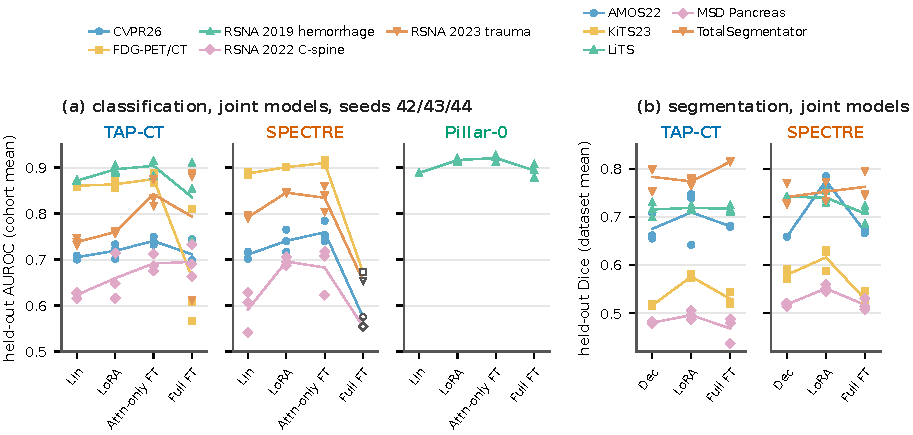
\includegraphics[width=\textwidth]{figures/fig_seeds.pdf}
\caption{Between-seed variation of the joint models next to between-method differences: cohort (dataset) means of the three seeds per method, (a) classification, (b) segmentation.}
\label{fig:seeds}
\end{figure}

\begin{table}[htbp]
\centering
\caption{Full fine-tuning settings and controls on the classification joint models: held-out AUROC per backbone and cohort for full fine-tuning with the default setting, a lower learning rate ($5\times10^{-6}$), layer-wise learning-rate decay (0.75 per block) and gradient accumulation with clipping, for MLP-only fine-tuning and for rsLoRA at a quarter of the learning rate, next to Lin and LoRA.}
\label{tab:revisioncls}
\adjustbox{max width=\textwidth}{\footnotesize\setlength{\tabcolsep}{3.5pt}
\begin{tabular}{@{}llccccccccc@{}}
\toprule
Backbone & Cohort (labels) & Lin & LoRA & \begin{tabular}[b]{@{}c@{}}Full\\FT\end{tabular} & \begin{tabular}[b]{@{}c@{}}Full FT,\\lower LR\end{tabular} & \begin{tabular}[b]{@{}c@{}}Full FT,\\layer decay\end{tabular} & \begin{tabular}[b]{@{}c@{}}Full FT,\\accumulation\end{tabular} & \begin{tabular}[b]{@{}c@{}}MLP-only\\FT\end{tabular} & rsLoRA & \begin{tabular}[b]{@{}c@{}}rsLoRA,\\matched LR\end{tabular} \\
\midrule
TAP-CT & CVPR26 (17) & 0.707 & 0.733 & 0.744 & 0.730 & \textbf{0.750} & 0.685 & \underline{0.745} & 0.722 & 0.741 \\
 & FDG-PET/CT (4) & 0.858 & \underline{0.866} & 0.608 & 0.861 & \textbf{0.867} & \textbf{0.867} & \underline{0.866} & 0.785 & 0.855 \\
 & RSNA 2022 C-spine (8) & 0.626 & \underline{0.714} & \textbf{0.732} & 0.654 & 0.618 & 0.687 & 0.627 & 0.601 & 0.611 \\
 & RSNA 2023 trauma (4) & 0.739 & 0.757 & \underline{0.881} & 0.860 & 0.869 & 0.758 & \textbf{0.894} & 0.684 & 0.751 \\
 & RSNA 2019 hemorrhage (6) & 0.871 & 0.906 & 0.854 & 0.889 & \textbf{0.917} & \underline{0.909} & 0.907 & 0.869 & 0.901 \\
\addlinespace
SPECTRE & CVPR26 (17) & 0.702 & 0.716 & 0.575$^{\dagger}$ & 0.713 & \textbf{0.758} & 0.511 & 0.681 & 0.690 & \underline{0.739} \\
 & FDG-PET/CT (4) & 0.884 & \underline{0.901} & 0.673$^{\dagger}$ & 0.884 & 0.865 & 0.883 & 0.814 & 0.900 & \textbf{0.908} \\
 & RSNA 2022 C-spine (8) & 0.629 & \textbf{0.706} & 0.554$^{\dagger}$ & 0.568 & \underline{0.700} & 0.553 & 0.626 & 0.691 & 0.672 \\
 & RSNA 2023 trauma (4) & 0.789 & 0.846 & 0.654$^{\dagger}$ & 0.793 & \textbf{0.863} & 0.578 & 0.838 & \underline{0.850} & 0.834 \\
\addlinespace
Pillar-0 & RSNA 2019 hemorrhage (6) & 0.888 & 0.912 & 0.878 & \textbf{0.924} & \underline{0.920} & 0.918 & 0.912 & 0.918 & \underline{0.920} \\
\bottomrule
\end{tabular}
}
\end{table}

\begin{table}[htbp]
\centering
\caption{Compute-matched segmentation: dataset-mean held-out Dice of the 24\,000-step joint model, of per-structure models trained for 1600 steps each (the same total number of steps) and their difference, for Dec, LoRA and Full FT on AMOS22 and TotalSegmentator.}
\label{tab:computematched}
\adjustbox{max width=\textwidth}{\footnotesize\begin{tabular}{@{}lllcccc@{}}
\toprule
Dataset (structures) & Backbone & Method & \begin{tabular}[b]{@{}c@{}}Joint\\{\scriptsize 24\,000 steps}\end{tabular} & \begin{tabular}[b]{@{}c@{}}Per-task, matched\\{\scriptsize 1600 steps each}\end{tabular} & Joint $-$ matched & \begin{tabular}[b]{@{}c@{}}Per-task\\{\scriptsize 8000 steps each}\end{tabular} \\
\midrule
AMOS22 (15) & TAP-CT & Dec & 0.708 & 0.763 & -0.055 & 0.793 \\
 &  & LoRA & 0.739 & 0.617 & +0.122 & 0.767 \\
 &  & Full FT & 0.681 & 0.766 & -0.085 & 0.805 \\
\addlinespace[2pt]
 & SPECTRE & Dec & 0.658 & 0.760 & -0.101 & 0.808 \\
 &  & LoRA & 0.784 & 0.648 & +0.136 & 0.812 \\
 &  & Full FT & 0.669 & 0.793 & -0.123 & 0.792 \\
\addlinespace
TotalSegmentator (15) & TAP-CT & Dec & 0.798 & 0.783 & +0.015 & 0.843 \\
 &  & LoRA & 0.776 & 0.657 & +0.119 & 0.819 \\
 &  & Full FT & 0.815 & 0.803 & +0.012 & 0.832 \\
\addlinespace[2pt]
 & SPECTRE & Dec & 0.770 & 0.806 & -0.037 & 0.848 \\
 &  & LoRA & 0.733 & 0.691 & +0.042 & 0.848 \\
 &  & Full FT & 0.795 & 0.819 & -0.024 & 0.838 \\
\bottomrule
\end{tabular}
}
\end{table}

\begin{table}[htbp]
\centering
\caption{From-scratch control: TAP-CT architecture with a randomly initialised encoder, trained as the Full FT joint model, next to Full FT and Dec, per dataset (held-out Dice, mean over structures).}
\label{tab:scratch}
\adjustbox{max width=\textwidth}{\footnotesize\begin{tabular}{@{}lccccc@{}}
\toprule
Dataset (structures) & From scratch & Dec & Full FT & Scratch $-$ Dec & Scratch $-$ Full FT \\
\midrule
AMOS22 (15) & 0.496 & 0.708 & 0.681 & -0.212 & -0.185 \\
KiTS23 (3) & 0.400 & 0.514 & 0.519 & -0.114 & -0.120 \\
LiTS (2) & 0.612 & 0.699 & 0.715 & -0.087 & -0.103 \\
MSD Pancreas (2) & 0.308 & 0.480 & 0.487 & -0.172 & -0.180 \\
TotalSegmentator (15) & 0.579 & 0.798 & 0.815 & -0.219 & -0.236 \\
\bottomrule
\end{tabular}
}
\end{table}

\begin{figure}[htbp]
\centering
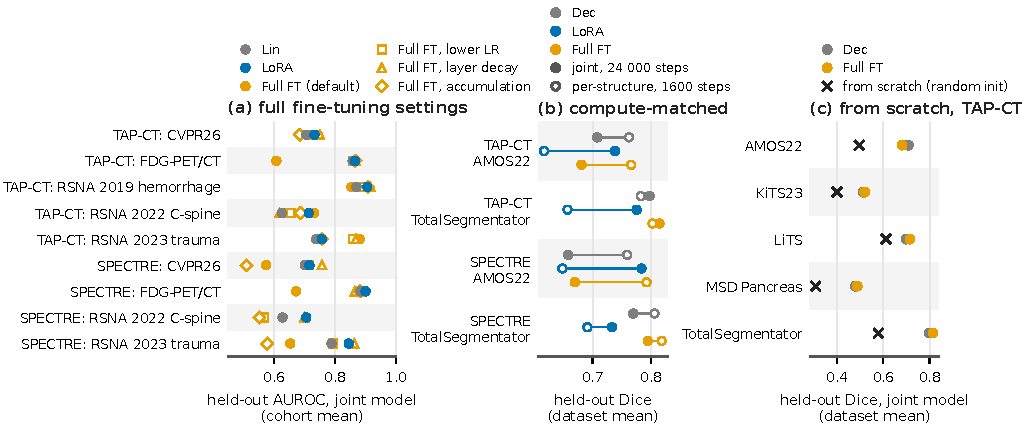
\includegraphics[width=\textwidth]{figures/fig_revision.pdf}
\caption{Repeats and controls. (a) Full fine-tuning settings against Lin and LoRA on the classification joint models. (b) Compute-matched segmentation: joint model against per-structure models at 1600 steps. (c) From-scratch control against Full FT and Dec on TAP-CT.}
\label{fig:revision}
\end{figure}

\begin{figure}[htbp]
\centering
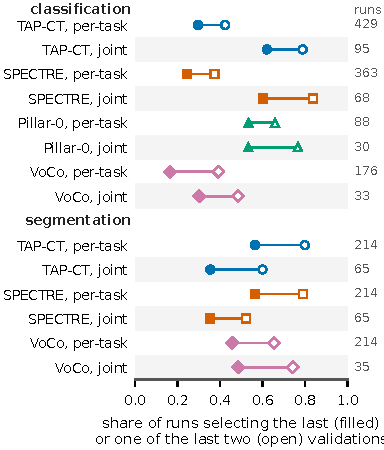
\includegraphics[width=\textwidth]{figures/fig_convergence.pdf}
\caption{Share of runs whose selected checkpoint is the last validation or one of the last two, per task and backbone.}
\label{fig:convergence}
\end{figure}

\begin{table}[htbp]
\centering
\caption{Convergence: share of runs that selected the last validation or one of the last two, per task and backbone.}
\label{tab:convergence}
\adjustbox{max width=\textwidth}{\small\begin{tabular}{@{}llrcc@{}}
\toprule
Backbone & Mode & Runs & \begin{tabular}[b]{@{}c@{}}Last validation\\{\scriptsize selected (\%)}\end{tabular} & \begin{tabular}[b]{@{}c@{}}One of last two\\{\scriptsize selected (\%)}\end{tabular} \\
\midrule
\multicolumn{5}{@{}l}{\textit{Classification}} \\
TAP-CT & per-task & 429 & 30 & 42 \\
 & joint & 120 & 64 & 79 \\
 & joint (26\,000 steps) & 11 & 9 & 9 \\
\addlinespace[2pt]
SPECTRE & per-task & 363 & 25 & 37 \\
 & joint & 88 & 56 & 78 \\
 & joint (26\,000 steps) & 11 & 18 & 27 \\
\addlinespace[2pt]
Pillar-0 & per-task & 88 & 53 & 66 \\
 & joint & 35 & 60 & 80 \\
\addlinespace[2pt]
VoCo & per-task & 176 & 16 & 39 \\
 & joint & 33 & 30 & 48 \\
\addlinespace[2pt]
All & all & 1354 & 33 & 49 \\
\addlinespace
\multicolumn{5}{@{}l}{\textit{Segmentation}} \\
TAP-CT & per-task & 214 & 57 & 80 \\
 & joint & 70 & 34 & 63 \\
 & joint (8000 steps) & 14 & 79 & 93 \\
 & per-task, compute-matched & 90 & 49 & 74 \\
\addlinespace[2pt]
SPECTRE & per-task & 214 & 57 & 79 \\
 & joint & 65 & 35 & 52 \\
 & joint (8000 steps) & 14 & 93 & 100 \\
 & per-task, compute-matched & 90 & 66 & 90 \\
\addlinespace[2pt]
VoCo & per-task & 214 & 46 & 65 \\
 & joint & 35 & 49 & 74 \\
 & joint (8000 steps) & 14 & 64 & 86 \\
\addlinespace[2pt]
All & all & 1034 & 52 & 75 \\
\bottomrule
\end{tabular}
}
\end{table}

\section{VoCo}
\label{app:voco}

\begin{table}[htbp]
\centering
\caption{The comparisons of Table~\ref{tab:key} on VoCo (\numLabelsVocoN{} labels from FDG-PET/CT, RSNA 2022 and RSNA 2023; all \numStructsVocoN{} structures).}
\label{tab:keyvoco}
\adjustbox{max width=\textwidth}{\small\begin{tabular}{@{}lcc@{}}
\toprule
Comparison & VoCo & Cohorts $>0$ \\
\midrule
\multicolumn{3}{@{}l}{\textit{Classification (AUROC)}} \\
LoRA $-$ Lin & \mci{-0.071}{-0.168}{-0.005} & 0/3 \\
LoRA $-$ Attn & \mci{-0.031}{-0.145}{+0.043} & 1/3 \\
Attn-only FT $-$ LoRA & \mci{+0.036}{-0.024}{+0.102} & 2/3 \\
Full FT $-$ Lin & \mci{-0.034}{-0.136}{+0.027} & 1/3 \\
joint $-$ per-task & \mci{-0.001}{-0.022}{+0.018} & 2/3 \\
\addlinespace
\multicolumn{3}{@{}l}{\textit{Segmentation (Dice)}} \\
Dec $-$ Lin & \mci{+0.680}{+0.433}{+0.746} & 5/5 \\
LoRA $-$ Dec & \mci{-0.018}{-0.047}{+0.016} & 2/5 \\
LoRA $-$ Dec, per-task & \mci{-0.035}{-0.062}{-0.007} & 0/5 \\
LoRA $-$ Dec, joint & \mci{0.000}{-0.034}{+0.047} & 2/5 \\
Full FT $-$ Dec & \mci{+0.015}{+0.007}{+0.023} & 4/5 \\
joint $-$ per-task & \mci{-0.041}{-0.081}{+0.004} & 2/5 \\
\bottomrule
\end{tabular}
}
\end{table}

\begin{table}[htbp]
\centering
\caption{VoCo classification: held-out AUROC as in Table~\ref{tab:cls}.}
\label{tab:clsvoco}
\adjustbox{max width=\textwidth}{\footnotesize\setlength{\tabcolsep}{3pt}
\begin{tabular}{@{}lllccccccccccc@{}}
\toprule
Cohort (labels) & Backbone & Mode & Lin & Attn & LoRA & LoRA$_{\text{late}}$ & \begin{tabular}[b]{@{}c@{}}LoRA+\\ABMIL\end{tabular} & DoRA & rsLoRA & \begin{tabular}[b]{@{}c@{}}Lin$\to$\\LoRA\end{tabular} & \begin{tabular}[b]{@{}c@{}}Attn$\to$\\LoRA\end{tabular} & \begin{tabular}[b]{@{}c@{}}Attn-only\\FT\end{tabular} & \begin{tabular}[b]{@{}c@{}}Full\\FT\end{tabular} \\
\midrule
FDG-PET/CT (4) & VoCo & per-task & \underline{0.720} & 0.685 & 0.512 & \cellcolor{modebest}0.671 & 0.562 & \cellcolor{modebest}0.669 & \cellcolor{modebest}0.598 & \textbf{0.736} & \cellcolor{modebest}0.591 & \cellcolor{modebest}0.665 & \cellcolor{modebest}0.606 \\
 &  & joint & \cellcolor{modebest}\underline{0.745} & \cellcolor{modebest}0.739 & \cellcolor{modebest}0.600 & 0.506 & \cellcolor{modebest}0.655 & 0.564 & 0.527 & \cellcolor{modebest}\textbf{0.750} & 0.520 & 0.641 & 0.582 \\
\addlinespace
RSNA 2022 C-spine (8) & VoCo & per-task & \cellcolor{modebest}\underline{0.606} & 0.508 & 0.537 & \cellcolor{modebest}0.551 & \cellcolor{modebest}0.596 & 0.561 & \cellcolor{modebest}\textbf{0.617} & 0.602 & 0.521 & 0.576 & \cellcolor{modebest}0.605 \\
 &  & joint & 0.586 & \cellcolor{modebest}0.548 & \cellcolor{modebest}0.560 & 0.550 & 0.565 & \cellcolor{modebest}0.589 & 0.578 & \cellcolor{modebest}\textbf{0.619} & \cellcolor{modebest}0.527 & \cellcolor{modebest}0.589 & \underline{0.593} \\
\addlinespace
RSNA 2023 trauma (4) & VoCo & per-task & 0.617 & \cellcolor{modebest}\underline{0.625} & \cellcolor{modebest}0.622 & 0.601 & \cellcolor{modebest}0.595 & \cellcolor{modebest}0.611 & \cellcolor{modebest}0.608 & \cellcolor{modebest}\textbf{0.631} & 0.569 & 0.588 & 0.596 \\
 &  & joint & \cellcolor{modebest}0.631 & 0.616 & 0.603 & \cellcolor{modebest}0.627 & 0.570 & 0.583 & 0.607 & 0.626 & \cellcolor{modebest}\underline{0.635} & \cellcolor{modebest}0.593 & \cellcolor{modebest}\textbf{0.648} \\
\bottomrule
\end{tabular}
}
\end{table}

\begin{table}[htbp]
\centering
\caption{VoCo segmentation: held-out Dice as in Table~\ref{tab:seg}.}
\label{tab:segvoco}
\adjustbox{max width=\textwidth}{\footnotesize\setlength{\tabcolsep}{3pt}
\begin{tabular}{@{}lllccccccc@{}}
\toprule
Dataset (structures) & Backbone & Mode & Lin & Dec & LoRA & LoRA$_{\text{late}}$ & DoRA & \begin{tabular}[b]{@{}c@{}}Full\\FT\end{tabular} & \begin{tabular}[b]{@{}c@{}}Dec$\to$\\LoRA\end{tabular} \\
\midrule
AMOS22 (15) & VoCo & per-task & \cellcolor{modebest}0.041 & \cellcolor{modebest}\underline{0.805} & \cellcolor{modebest}0.782 & \cellcolor{modebest}0.783 & \cellcolor{modebest}0.783 & \cellcolor{modebest}\textbf{0.818} & \cellcolor{modebest}0.799 \\
 &  & joint & 0.038 & 0.739 & \underline{0.762} & 0.758 & \textbf{0.764} & 0.752 & 0.736 \\
\addlinespace
KiTS23 (3) & VoCo & per-task & 0.017 & \cellcolor{modebest}\underline{0.519} & 0.501 & 0.500 & 0.493 & \cellcolor{modebest}\textbf{0.564} & \cellcolor{modebest}0.481 \\
 &  & joint & \cellcolor{modebest}0.037 & 0.465 & 0.501 & \cellcolor{modebest}\textbf{0.516} & \cellcolor{modebest}\underline{0.507} & 0.481 & 0.452 \\
\addlinespace
LiTS (2) & VoCo & per-task & 0.342 & \cellcolor{modebest}\underline{0.733} & 0.692 & 0.694 & 0.688 & \cellcolor{modebest}\textbf{0.748} & 0.720 \\
 &  & joint & \cellcolor{modebest}0.345 & \underline{0.732} & \cellcolor{modebest}0.720 & \cellcolor{modebest}0.710 & \cellcolor{modebest}0.718 & \textbf{0.737} & \cellcolor{modebest}0.726 \\
\addlinespace
MSD Pancreas (2) & VoCo & per-task & 0.000 & \cellcolor{modebest}\textbf{0.569} & 0.539 & 0.545 & 0.541 & \cellcolor{modebest}\underline{0.566} & 0.558 \\
 &  & joint & 0.000 & 0.559 & \cellcolor{modebest}0.552 & 0.545 & \cellcolor{modebest}0.552 & \underline{0.560} & \cellcolor{modebest}\textbf{0.561} \\
\addlinespace
TotalSegmentator (15) & VoCo & per-task & \cellcolor{modebest}0.055 & \cellcolor{modebest}\underline{0.822} & \cellcolor{modebest}0.771 & -- & -- & \cellcolor{modebest}\textbf{0.838} & -- \\
 &  & joint & 0.047 & \underline{0.732} & 0.705 & 0.697 & 0.709 & \textbf{0.750} & 0.723 \\
\bottomrule
\end{tabular}
}
\end{table}

\begin{figure}[htbp]
\centering
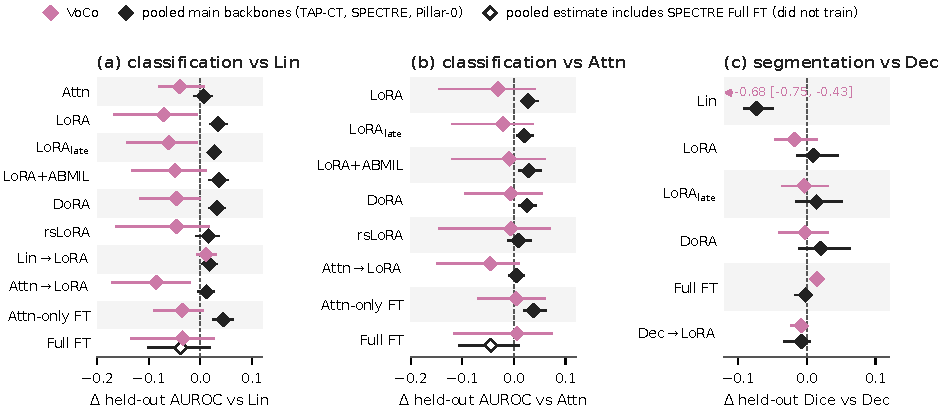
\includegraphics[width=\textwidth]{figures/fig_voco.pdf}
\caption{VoCo. (a) Label-level difference of every classification method to the linear probe on VoCo, next to the estimate pooled over the main backbones. (b) Per-structure change in held-out Dice relative to the frozen decoder on VoCo.}
\label{fig:voco}
\end{figure}

\begin{table}[htbp]
\centering
\caption{Median over label--mode pairs of the standard deviation of the held-out probabilities per backbone and method (the did-not-train rule flags values below \numSpreadMinValue{}; applied to TAP-CT, SPECTRE and Pillar-0 only).}
\label{tab:spread}
\adjustbox{max width=\textwidth}{\small\setlength{\tabcolsep}{3pt}
\begin{tabular}{lccccccccccc}
\toprule
Backbone & Lin & Attn & LoRA & LoRA$_{\text{late}}$ & LoRA+ABMIL & DoRA & rsLoRA & Lin$\to$LoRA & Attn$\to$LoRA & Attn-only FT & Full FT \\
\midrule
TAP-CT & 0.227 & 0.239 & 0.239 & 0.235 & 0.233 & 0.237 & 0.167 & 0.222 & 0.225 & 0.247 & 0.170 \\
SPECTRE & 0.187 & 0.114 & 0.161 & 0.185 & 0.187 & 0.185 & 0.150 & 0.178 & 0.129 & 0.148 & \textbf{0.004}$^{\dagger}$ \\
Pillar-0 & 0.294 & 0.321 & 0.359 & 0.350 & 0.352 & 0.354 & 0.359 & 0.337 & 0.338 & 0.355 & 0.347 \\
VoCo & 0.152 & 0.023 & 0.035 & 0.032 & 0.008 & 0.030 & 0.036 & 0.150 & 0.020 & 0.041 & 0.036 \\
\bottomrule
\end{tabular}
}
\end{table}

\section{Ranks, paired tests and per-label results}
\label{app:perlabel}

\begin{figure}[htbp]
\centering
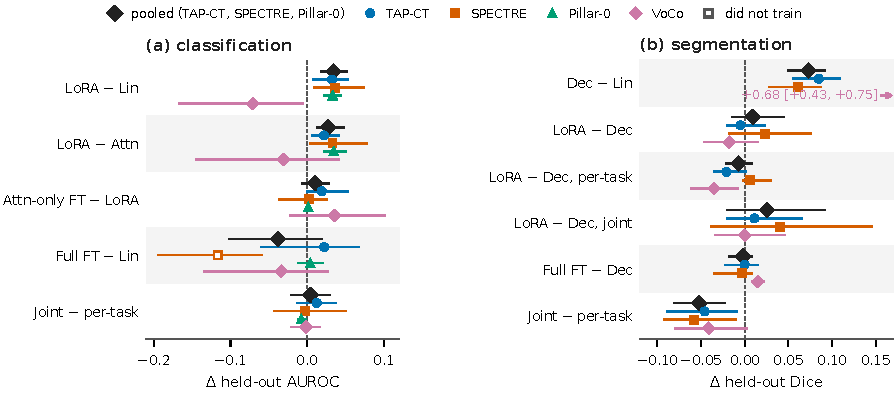
\includegraphics[width=\textwidth]{figures/fig_key.pdf}
\caption{The comparisons of Table~\ref{tab:key} per backbone: label-level mean difference in held-out AUROC (a) or Dice (b) with its 95\% interval; 0 means no difference. The black diamond pools TAP-CT, SPECTRE and Pillar-0; VoCo has its own marker and is never pooled.}
\label{fig:key}
\end{figure}

\begin{figure}[htbp]
\centering
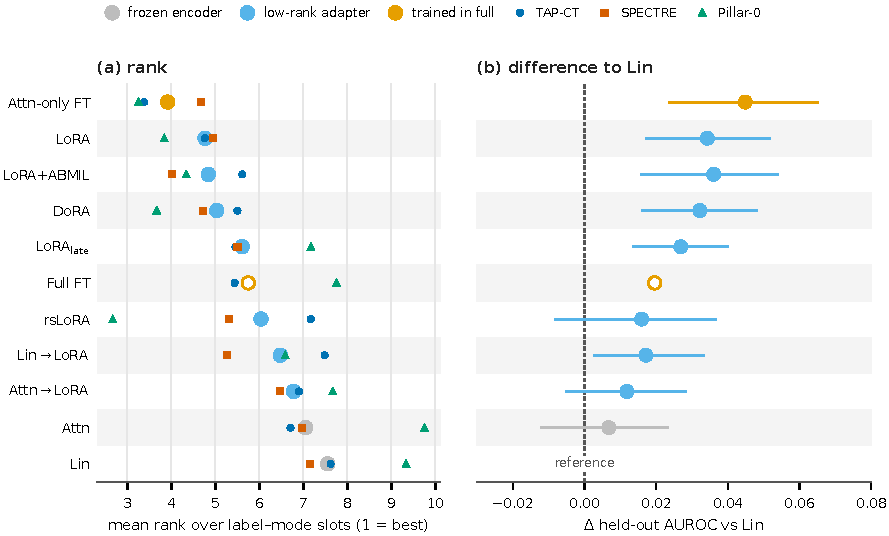
\includegraphics[width=\textwidth]{figures/fig_methods_cls_rank.pdf}
\caption{Classification methods on the three main backbones. (a) Mean rank over label--mode pairs, 1 = best; large markers pool the backbones, small markers are per backbone. (b) Label-level mean difference to the linear probe with its 95\% interval. SPECTRE Full FT, which did not train, is excluded from the ranks and drawn open in (b).}
\label{fig:ranks}
\end{figure}

\begin{figure}[htbp]
\centering
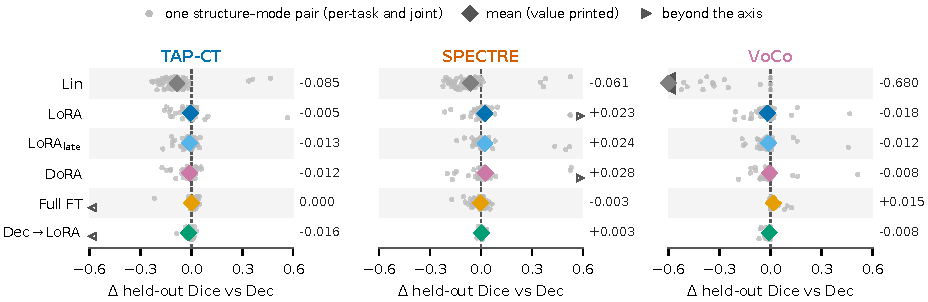
\includegraphics[width=\textwidth]{figures/fig_perstructure_seg.pdf}
\caption{Per-structure change in held-out Dice relative to the frozen decoder of the same backbone, dataset and mode (grey: structure--mode pairs; coloured: mean, printed on the right; open triangles: beyond the axis), for TAP-CT, SPECTRE and VoCo.}
\label{fig:perstructure}
\end{figure}

\begin{table}[htbp]
\centering
\caption{Classification: held-out AUROC, mean over the labels of each cohort (number of labels in brackets), per backbone, training mode and method. Best results are bolded, while second-best results are underlined. A \colorbox{modebest}{shaded} cell marks the better of per-task and joint training for that method, backbone and cohort. SPECTRE Full FT did not train with the default setting (Section~\ref{sec:fullft}) and is not marked.}
\label{tab:cls}
\adjustbox{max width=\textwidth}{\footnotesize\setlength{\tabcolsep}{3pt}
\begin{tabular}{@{}lllccccccccccc@{}}
\toprule
Cohort (labels) & Backbone & Mode & Lin & Attn & LoRA & LoRA$_{\text{late}}$ & \begin{tabular}[b]{@{}c@{}}LoRA+\\ABMIL\end{tabular} & DoRA & rsLoRA & \begin{tabular}[b]{@{}c@{}}Lin$\to$\\LoRA\end{tabular} & \begin{tabular}[b]{@{}c@{}}Attn$\to$\\LoRA\end{tabular} & \begin{tabular}[b]{@{}c@{}}Attn-only\\FT\end{tabular} & \begin{tabular}[b]{@{}c@{}}Full\\FT\end{tabular} \\
\midrule
CVPR26 (17) & TAP-CT & per-task & 0.677 & 0.718 & \underline{0.732} & 0.704 & 0.728 & 0.717 & \cellcolor{modebest}0.724 & \cellcolor{modebest}0.697 & 0.707 & \cellcolor{modebest}\textbf{0.744} & 0.720 \\
 &  & joint & \cellcolor{modebest}0.707 & \cellcolor{modebest}0.720 & \cellcolor{modebest}0.733 & \cellcolor{modebest}0.726 & \cellcolor{modebest}0.729 & \cellcolor{modebest}0.733 & 0.722 & 0.695 & \cellcolor{modebest}0.708 & \underline{0.739} & \cellcolor{modebest}\textbf{0.744} \\
\addlinespace[1.5pt]
 & SPECTRE & per-task & \cellcolor{modebest}0.736 & 0.725 & \cellcolor{modebest}0.769 & \cellcolor{modebest}0.769 & \cellcolor{modebest}\underline{0.776} & \cellcolor{modebest}0.766 & \cellcolor{modebest}0.768 & \cellcolor{modebest}0.769 & \cellcolor{modebest}0.765 & \cellcolor{modebest}\textbf{0.778} & 0.627$^{\dagger}$ \\
 &  & joint & 0.702 & \cellcolor{modebest}0.738 & 0.716 & 0.731 & \textbf{0.747} & 0.731 & 0.690 & \underline{0.744} & 0.728 & 0.740 & 0.575$^{\dagger}$ \\
\addlinespace
FDG-PET/CT (4) & TAP-CT & per-task & \cellcolor{modebest}0.863 & 0.836 & 0.852 & \cellcolor{modebest}\textbf{0.868} & 0.839 & 0.847 & \cellcolor{modebest}0.817 & \cellcolor{modebest}\underline{0.866} & 0.856 & 0.832 & \cellcolor{modebest}0.769 \\
 &  & joint & 0.858 & \cellcolor{modebest}0.860 & \cellcolor{modebest}\underline{0.866} & 0.864 & \cellcolor{modebest}0.849 & \cellcolor{modebest}0.858 & 0.785 & 0.860 & \cellcolor{modebest}0.862 & \cellcolor{modebest}\textbf{0.870} & 0.608 \\
\addlinespace[1.5pt]
 & SPECTRE & per-task & 0.857 & 0.862 & 0.882 & 0.879 & 0.874 & \textbf{0.892} & 0.872 & \cellcolor{modebest}\underline{0.887} & 0.867 & 0.848 & 0.617$^{\dagger}$ \\
 &  & joint & \cellcolor{modebest}0.884 & \cellcolor{modebest}0.880 & \cellcolor{modebest}\underline{0.901} & \cellcolor{modebest}0.888 & \cellcolor{modebest}0.889 & \cellcolor{modebest}0.900 & \cellcolor{modebest}0.900 & 0.884 & \cellcolor{modebest}0.884 & \cellcolor{modebest}\textbf{0.906} & 0.673$^{\dagger}$ \\
\addlinespace
RSNA 2022 C-spine (8) & TAP-CT & per-task & 0.619 & \cellcolor{modebest}0.625 & 0.623 & 0.608 & 0.613 & \underline{0.641} & \cellcolor{modebest}0.635 & 0.606 & \cellcolor{modebest}0.629 & \textbf{0.660} & 0.637 \\
 &  & joint & \cellcolor{modebest}0.626 & 0.624 & \cellcolor{modebest}\underline{0.714} & \cellcolor{modebest}0.706 & \cellcolor{modebest}0.713 & \cellcolor{modebest}0.680 & 0.601 & \cellcolor{modebest}0.624 & 0.620 & \cellcolor{modebest}0.712 & \cellcolor{modebest}\textbf{0.732} \\
\addlinespace[1.5pt]
 & SPECTRE & per-task & 0.579 & 0.591 & 0.635 & \cellcolor{modebest}\textbf{0.654} & \underline{0.644} & 0.619 & 0.638 & 0.615 & 0.591 & 0.635 & 0.566$^{\dagger}$ \\
 &  & joint & \cellcolor{modebest}0.629 & \cellcolor{modebest}0.601 & \cellcolor{modebest}0.706 & 0.644 & \cellcolor{modebest}\textbf{0.730} & \cellcolor{modebest}0.692 & \cellcolor{modebest}0.691 & \cellcolor{modebest}0.670 & \cellcolor{modebest}0.611 & \cellcolor{modebest}\underline{0.718} & 0.554$^{\dagger}$ \\
\addlinespace
RSNA 2023 trauma (4) & TAP-CT & per-task & 0.737 & 0.718 & 0.739 & \cellcolor{modebest}0.756 & 0.703 & 0.752 & \cellcolor{modebest}0.725 & 0.738 & 0.716 & \cellcolor{modebest}\textbf{0.859} & \underline{0.775} \\
 &  & joint & \cellcolor{modebest}0.739 & \cellcolor{modebest}0.738 & \cellcolor{modebest}0.757 & 0.744 & \cellcolor{modebest}0.758 & \cellcolor{modebest}0.768 & 0.684 & \cellcolor{modebest}0.746 & \cellcolor{modebest}0.758 & \underline{0.833} & \cellcolor{modebest}\textbf{0.881} \\
\addlinespace[1.5pt]
 & SPECTRE & per-task & \cellcolor{modebest}0.791 & 0.778 & 0.824 & 0.832 & \textbf{0.852} & \cellcolor{modebest}\underline{0.842} & 0.836 & 0.825 & 0.798 & 0.772 & 0.624$^{\dagger}$ \\
 &  & joint & 0.789 & \cellcolor{modebest}0.788 & \cellcolor{modebest}0.846 & \cellcolor{modebest}0.835 & \cellcolor{modebest}\textbf{0.859} & 0.838 & \cellcolor{modebest}\underline{0.850} & \cellcolor{modebest}0.827 & \cellcolor{modebest}0.810 & \cellcolor{modebest}0.803 & 0.654$^{\dagger}$ \\
\addlinespace
RSNA 2019 hemorrhage (6) & TAP-CT & per-task & 0.870 & 0.873 & 0.894 & 0.894 & \cellcolor{modebest}0.891 & \underline{0.897} & \cellcolor{modebest}0.870 & \cellcolor{modebest}0.877 & \cellcolor{modebest}0.878 & \textbf{0.911} & \cellcolor{modebest}0.888 \\
 &  & joint & \cellcolor{modebest}0.871 & \cellcolor{modebest}0.877 & \cellcolor{modebest}\underline{0.906} & \cellcolor{modebest}0.895 & 0.886 & 0.897 & 0.869 & 0.868 & 0.876 & \cellcolor{modebest}\textbf{0.915} & 0.854 \\
\addlinespace[1.5pt]
 & Pillar-0 & per-task & 0.886 & 0.884 & \cellcolor{modebest}\underline{0.929} & \cellcolor{modebest}0.914 & 0.902 & \cellcolor{modebest}\textbf{0.931} & \cellcolor{modebest}0.920 & \cellcolor{modebest}0.912 & \cellcolor{modebest}0.903 & \cellcolor{modebest}\textbf{0.931} & \cellcolor{modebest}0.904 \\
 &  & joint & \cellcolor{modebest}0.888 & \cellcolor{modebest}0.888 & 0.912 & 0.892 & \cellcolor{modebest}\textbf{0.925} & 0.912 & \underline{0.918} & 0.905 & 0.898 & 0.912 & 0.878 \\
\bottomrule
\end{tabular}
}
\end{table}

\begin{figure}[htbp]
\centering
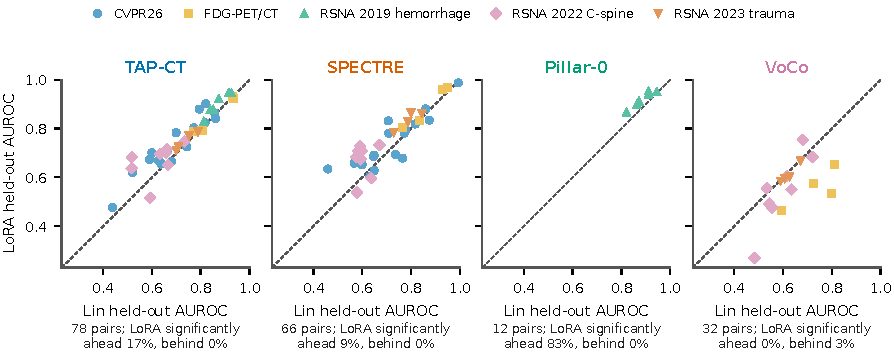
\includegraphics[width=\textwidth]{figures/fig_perlabel_cls.pdf}
\caption{Held-out AUROC of LoRA against the linear probe per label and mode, one panel per backbone; points above the identity line favour LoRA. The text under each panel gives the share of label--mode pairs in which LoRA is significantly ahead or behind.}
\label{fig:perlabel}
\end{figure}

\begin{table}[htbp]
\centering
\caption{Segmentation: held-out Dice, mean over the structures of each dataset (number of structures in brackets), per backbone, training mode and method; -- marks methods not run per structure on TotalSegmentator. Best results are bolded, while second-best results are underlined. A \colorbox{modebest}{shaded} cell marks the better of per-structure and joint training for that method, backbone and dataset. The AMOS22 and TotalSegmentator joint models train 24\,000 steps; their 8000-step runs are in Table~\ref{tab:segmodes}.}
\label{tab:seg}
\adjustbox{max width=\textwidth}{\footnotesize\setlength{\tabcolsep}{3pt}
\begin{tabular}{@{}lllccccccc@{}}
\toprule
Dataset (structures) & Backbone & Mode & Lin & Dec & LoRA & LoRA$_{\text{late}}$ & DoRA & \begin{tabular}[b]{@{}c@{}}Full\\FT\end{tabular} & \begin{tabular}[b]{@{}c@{}}Dec$\to$\\LoRA\end{tabular} \\
\midrule
AMOS22 (15) & TAP-CT & per-task & \cellcolor{modebest}0.658 & \cellcolor{modebest}\underline{0.793} & \cellcolor{modebest}0.767 & \cellcolor{modebest}0.764 & \cellcolor{modebest}0.761 & \cellcolor{modebest}\textbf{0.805} & \cellcolor{modebest}0.791 \\
 &  & joint & 0.646 & \underline{0.708} & \textbf{0.739} & 0.698 & \underline{0.708} & 0.681 & 0.656 \\
\addlinespace[1.5pt]
 & SPECTRE & per-task & \cellcolor{modebest}0.683 & \cellcolor{modebest}0.808 & \cellcolor{modebest}\underline{0.812} & \cellcolor{modebest}0.806 & \cellcolor{modebest}\textbf{0.814} & \cellcolor{modebest}0.792 & \cellcolor{modebest}\textbf{0.814} \\
 &  & joint & 0.682 & 0.658 & \textbf{0.784} & 0.764 & \underline{0.775} & 0.669 & 0.664 \\
\addlinespace
KiTS23 (3) & TAP-CT & per-task & \cellcolor{modebest}0.531 & \cellcolor{modebest}0.584 & 0.563 & \cellcolor{modebest}0.567 & \cellcolor{modebest}0.563 & \cellcolor{modebest}\textbf{0.588} & \cellcolor{modebest}\underline{0.587} \\
 &  & joint & 0.430 & 0.514 & \cellcolor{modebest}\textbf{0.582} & 0.556 & \underline{0.560} & 0.519 & 0.500 \\
\addlinespace[1.5pt]
 & SPECTRE & per-task & \cellcolor{modebest}0.583 & \cellcolor{modebest}0.599 & \cellcolor{modebest}0.613 & \cellcolor{modebest}\underline{0.617} & \cellcolor{modebest}\textbf{0.622} & \cellcolor{modebest}0.528 & \cellcolor{modebest}0.603 \\
 &  & joint & 0.530 & 0.572 & \underline{0.588} & \underline{0.588} & \textbf{0.593} & 0.519 & 0.570 \\
\addlinespace
LiTS (2) & TAP-CT & per-task & \cellcolor{modebest}0.659 & \cellcolor{modebest}0.709 & \cellcolor{modebest}\textbf{0.716} & 0.709 & \cellcolor{modebest}\underline{0.714} & 0.710 & \cellcolor{modebest}\underline{0.714} \\
 &  & joint & 0.656 & 0.699 & \underline{0.715} & \cellcolor{modebest}\textbf{0.721} & 0.692 & \cellcolor{modebest}\underline{0.715} & 0.703 \\
\addlinespace[1.5pt]
 & SPECTRE & per-task & 0.688 & \underline{0.741} & \cellcolor{modebest}\textbf{0.756} & 0.723 & \cellcolor{modebest}\textbf{0.756} & \cellcolor{modebest}0.739 & 0.729 \\
 &  & joint & \cellcolor{modebest}0.696 & \cellcolor{modebest}0.742 & \textbf{0.753} & \cellcolor{modebest}0.736 & \underline{0.743} & 0.713 & \cellcolor{modebest}\underline{0.743} \\
\addlinespace
MSD Pancreas (2) & TAP-CT & per-task & \cellcolor{modebest}0.427 & \cellcolor{modebest}0.491 & \underline{0.504} & \cellcolor{modebest}0.501 & \cellcolor{modebest}0.502 & \cellcolor{modebest}\textbf{0.512} & \cellcolor{modebest}0.495 \\
 &  & joint & 0.334 & 0.480 & \cellcolor{modebest}\textbf{0.505} & 0.492 & \underline{0.493} & 0.487 & 0.468 \\
\addlinespace[1.5pt]
 & SPECTRE & per-task & \cellcolor{modebest}0.475 & \cellcolor{modebest}0.516 & \cellcolor{modebest}\textbf{0.563} & \cellcolor{modebest}0.538 & \cellcolor{modebest}\underline{0.557} & 0.516 & 0.518 \\
 &  & joint & 0.459 & 0.514 & \textbf{0.550} & 0.529 & \textbf{0.550} & \cellcolor{modebest}\underline{0.530} & \cellcolor{modebest}0.520 \\
\addlinespace
TotalSegmentator (15) & TAP-CT & per-task & \cellcolor{modebest}0.747 & \cellcolor{modebest}\textbf{0.843} & \cellcolor{modebest}0.819 & -- & -- & \cellcolor{modebest}\underline{0.832} & -- \\
 &  & joint & 0.740 & \underline{0.798} & 0.776 & 0.776 & 0.776 & \textbf{0.815} & 0.790 \\
\addlinespace[1.5pt]
 & SPECTRE & per-task & \cellcolor{modebest}0.731 & \cellcolor{modebest}\textbf{0.848} & \cellcolor{modebest}\textbf{0.848} & -- & -- & \cellcolor{modebest}\underline{0.838} & -- \\
 &  & joint & 0.722 & 0.770 & 0.733 & 0.752 & 0.736 & \textbf{0.795} & \underline{0.772} \\
\bottomrule
\end{tabular}
}
\end{table}

\begin{figure}[htbp]
\centering
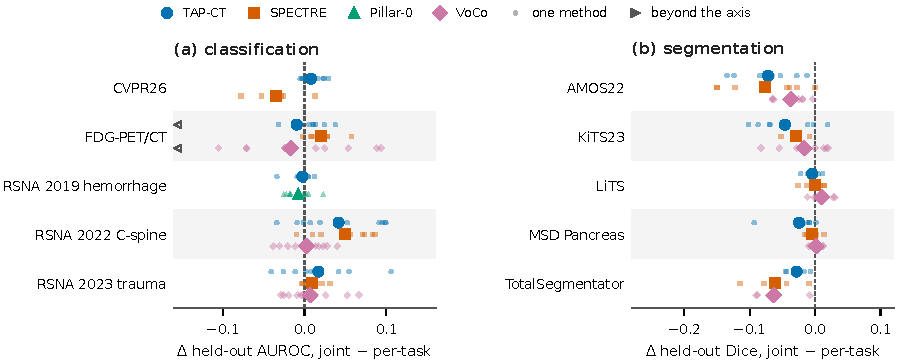
\includegraphics[width=\textwidth]{figures/fig_joint.pdf}
\caption{Joint minus per-task held-out AUROC per classification cohort (a) and joint minus per-structure held-out Dice per segmentation dataset (b), per backbone; small markers are methods, large markers their mean.}
\label{fig:joint}
\end{figure}

\begin{table}[htbp]
\centering
\caption{Classification: mean rank per method (1 = best) over the label--mode pairs with every method present, per backbone and pooled over the three main backbones; share of pairs within 0.01 AUROC of the best method and mean deficit to the best method.}
\label{tab:rankscls}
\adjustbox{max width=\textwidth}{\small\begin{tabular}{@{}lcccccc@{}}
\toprule
Method & \multicolumn{1}{c}{\begin{tabular}[b]{@{}c@{}}TAP-CT\\{\scriptsize 78 slots}\end{tabular}} & \multicolumn{1}{c}{\begin{tabular}[b]{@{}c@{}}SPECTRE\\{\scriptsize 66 slots}\end{tabular}} & \multicolumn{1}{c}{\begin{tabular}[b]{@{}c@{}}Pillar-0\\{\scriptsize 12 slots}\end{tabular}} & \multicolumn{1}{c}{\begin{tabular}[b]{@{}c@{}}All\\{\scriptsize 156 slots}\end{tabular}} & \begin{tabular}[b]{@{}c@{}}Within 0.01\\{\scriptsize of best (\%)}\end{tabular} & \begin{tabular}[b]{@{}c@{}}Regret\\{\scriptsize all}\end{tabular} \\
\midrule
Lin & 7.62 & 7.15 & 9.33 & 7.55 & 7 & 0.081 \\
Attn & 6.71 & 6.96 & 9.75 & 7.05 & 10 & 0.074 \\
LoRA & 4.76 & 4.94 & 3.83 & 4.76 & 23 & 0.046 \\
LoRA$_{\text{late}}$ & 5.46 & 5.50 & 7.17 & 5.61 & 17 & 0.054 \\
LoRA+ABMIL & 5.61 & \textbf{4.02} & 4.33 & 4.84 & 26 & 0.045 \\
DoRA & 5.50 & 4.72 & 3.67 & 5.03 & 19 & 0.049 \\
rsLoRA & 7.17 & 5.31 & \textbf{2.67} & 6.04 & 18 & 0.065 \\
Lin$\to$LoRA & 7.48 & 5.27 & 6.58 & 6.47 & 11 & 0.064 \\
Attn$\to$LoRA & 6.90 & 6.47 & 7.67 & 6.78 & 13 & 0.069 \\
Attn-only FT & \textbf{3.38} & 4.67 & 3.25 & \textbf{3.91} & \textbf{38} & \textbf{0.036} \\
Full FT & 5.44 & --$^{\dagger}$ & 7.75 & 5.74$^{\dagger}$ & 31 & 0.055 \\
\bottomrule
\end{tabular}
}
\end{table}

\begin{table}[htbp]
\centering
\caption{Segmentation: mean rank per method over the structure--mode pairs with all seven methods, per backbone and pooled.}
\label{tab:ranksseg}
\adjustbox{max width=\textwidth}{\small\begin{tabular}{@{}lccccc@{}}
\toprule
Method & \multicolumn{1}{c}{\begin{tabular}[b]{@{}c@{}}TAP-CT\\{\scriptsize 59 slots}\end{tabular}} & \multicolumn{1}{c}{\begin{tabular}[b]{@{}c@{}}SPECTRE\\{\scriptsize 59 slots}\end{tabular}} & \multicolumn{1}{c}{\begin{tabular}[b]{@{}c@{}}All\\{\scriptsize 118 slots}\end{tabular}} & \begin{tabular}[b]{@{}c@{}}Within 0.01\\{\scriptsize of best (\%)}\end{tabular} & \begin{tabular}[b]{@{}c@{}}Regret\\{\scriptsize all}\end{tabular} \\
\midrule
Lin & 6.49 & 6.25 & 6.37 & 4 & 0.116 \\
Dec & 3.70 & 4.35 & 4.03 & 21 & 0.051 \\
LoRA & 3.38 & 3.06 & 3.22 & 47 & \textbf{0.037} \\
LoRA$_{\text{late}}$ & 4.03 & 3.92 & 3.97 & 31 & 0.046 \\
DoRA & 3.91 & \textbf{2.86} & 3.38 & 44 & 0.043 \\
Full FT & \textbf{2.05} & 3.84 & \textbf{2.94} & \textbf{64} & 0.051 \\
Dec$\to$LoRA & 4.44 & 3.72 & 4.08 & 24 & 0.058 \\
\bottomrule
\end{tabular}
}
\end{table}

\begin{figure}[htbp]
\centering
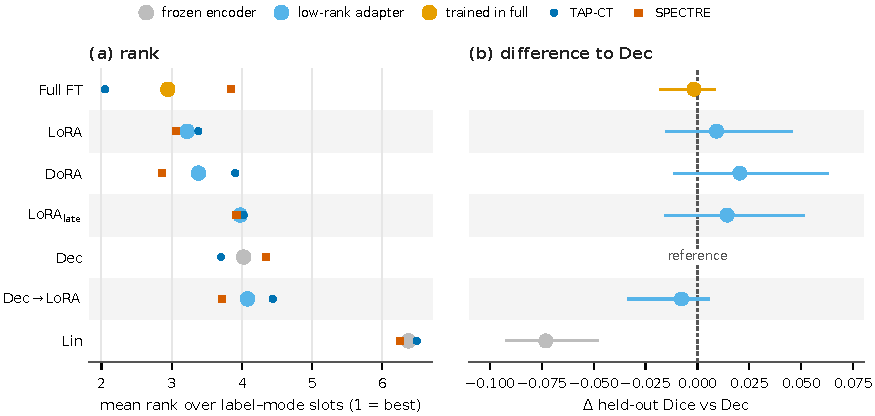
\includegraphics[width=\textwidth]{figures/fig_methods_seg_rank.pdf}
\caption{Segmentation methods on TAP-CT and SPECTRE. (a) Mean rank over structure--mode pairs, 1 = best. (b) Label-level mean difference to the frozen decoder with its 95\% interval.}
\label{fig:segranks}
\end{figure}

\begin{table}[htbp]
\centering
\caption{Label-level estimates for every comparison and backbone: number of labels, mean difference, 95\% interval over cohorts and labels, 95\% interval over cohorts, labels and held-out cases, and cohort--backbone clusters with a positive mean.}
\label{tab:cis}
\adjustbox{max width=\textwidth}{\footnotesize\begin{tabular}{@{}llrrccc@{}}
\toprule
Comparison & Backbone & $n$ & Mean & 95\% CI (two-stage) & 95\% CI (three-stage) & Cohorts $>0$ \\
\midrule
LoRA $-$ Lin & TAP-CT & 39 & +0.032 & [+0.009, +0.049] & [+0.007, +0.053] & 4/5 \\
 & SPECTRE & 33 & +0.037 & [+0.013, +0.068] & [+0.009, +0.075] & 4/4 \\
 & Pillar-0 & 6 & +0.033 & [+0.021, +0.042] & [+0.021, +0.044] & 1/1 \\
 & VoCo & 16 & -0.071 & [-0.162, -0.011] & [-0.168, -0.005] & 0/3 \\
 & All & 78 & +0.034 & [+0.019, +0.049] & [+0.017, +0.052] & 9/10 \\
\addlinespace[2pt]
LoRA $-$ Attn & TAP-CT & 39 & +0.022 & [+0.009, +0.039] & [+0.006, +0.042] & 5/5 \\
 & SPECTRE & 33 & +0.033 & [+0.007, +0.074] & [+0.003, +0.078] & 4/4 \\
 & Pillar-0 & 6 & +0.034 & [+0.021, +0.051] & [+0.021, +0.052] & 1/1 \\
 & VoCo & 16 & -0.031 & [-0.150, +0.033] & [-0.145, +0.043] & 1/3 \\
 & All & 78 & +0.027 & [+0.013, +0.047] & [+0.012, +0.048] & 10/10 \\
\addlinespace[2pt]
Attn-only FT $-$ LoRA & TAP-CT & 39 & +0.019 & [+0.002, +0.053] & [-0.001, +0.054] & 4/5 \\
 & SPECTRE & 33 & +0.002 & [-0.037, +0.023] & [-0.037, +0.026] & 2/4 \\
 & Pillar-0 & 6 & +0.001 & [0.000, +0.003] & [-0.002, +0.004] & 1/1 \\
 & VoCo & 16 & +0.036 & [-0.020, +0.097] & [-0.024, +0.102] & 2/3 \\
 & All & 78 & +0.011 & [-0.005, +0.026] & [-0.007, +0.029] & 7/10 \\
\addlinespace[2pt]
Full FT $-$ Lin & TAP-CT & 39 & +0.022 & [-0.057, +0.064] & [-0.061, +0.068] & 4/5 \\
 & SPECTRE & 33 & -0.117 & [-0.195, -0.063] & [-0.195, -0.059] & 0/4 \\
 & Pillar-0 & 6 & +0.004 & [-0.011, +0.019] & [-0.013, +0.021] & 1/1 \\
 & VoCo & 16 & -0.034 & [-0.133, +0.018] & [-0.136, +0.027] & 1/3 \\
 & All & 78 & -0.038 & [-0.101, +0.017] & [-0.103, +0.019] & 5/10 \\
\addlinespace[2pt]
joint $-$ per-task & TAP-CT & 39 & +0.012 & [-0.005, +0.032] & [-0.014, +0.038] & 3/5 \\
 & SPECTRE & 33 & -0.003 & [-0.035, +0.049] & [-0.044, +0.051] & 3/4 \\
 & Pillar-0 & 6 & -0.008 & [-0.012, -0.003] & [-0.013, -0.001] & 0/1 \\
 & VoCo & 16 & -0.001 & [-0.017, +0.012] & [-0.022, +0.018] & 2/3 \\
 & All & 78 & +0.004 & [-0.017, +0.027] & [-0.021, +0.030] & 6/10 \\
\addlinespace[2pt]
Attn $-$ Lin & TAP-CT & 39 & +0.011 & [-0.013, +0.027] & [-0.014, +0.029] & 3/5 \\
 & SPECTRE & 33 & +0.004 & [-0.022, +0.030] & [-0.030, +0.035] & 2/4 \\
 & Pillar-0 & 6 & -0.001 & [-0.012, +0.007] & [-0.014, +0.008] & 0/1 \\
 & VoCo & 16 & -0.040 & [-0.072, 0.000] & [-0.081, +0.008] & 0/3 \\
 & All & 78 & +0.007 & [-0.010, +0.021] & [-0.012, +0.023] & 5/10 \\
\addlinespace[2pt]
LoRA$_{\text{late}}$ $-$ Lin & TAP-CT & 39 & +0.023 & [+0.009, +0.036] & [+0.005, +0.039] & 5/5 \\
 & SPECTRE & 33 & +0.034 & [+0.016, +0.051] & [+0.011, +0.058] & 4/4 \\
 & Pillar-0 & 6 & +0.016 & [+0.008, +0.024] & [+0.007, +0.025] & 1/1 \\
 & VoCo & 16 & -0.061 & [-0.130, -0.010] & [-0.143, -0.005] & 0/3 \\
 & All & 78 & +0.027 & [+0.016, +0.038] & [+0.013, +0.040] & 10/10 \\
\addlinespace[2pt]
LoRA+ABMIL $-$ Lin & TAP-CT & 39 & +0.024 & [-0.006, +0.042] & [-0.005, +0.045] & 3/5 \\
 & SPECTRE & 33 & +0.052 & [+0.025, +0.080] & [+0.022, +0.086] & 4/4 \\
 & Pillar-0 & 6 & +0.026 & [+0.016, +0.037] & [+0.015, +0.038] & 1/1 \\
 & VoCo & 16 & -0.049 & [-0.134, -0.001] & [-0.134, +0.012] & 0/3 \\
 & All & 78 & +0.036 & [+0.018, +0.052] & [+0.016, +0.054] & 8/10 \\
\addlinespace[2pt]
DoRA $-$ Lin & TAP-CT & 39 & +0.028 & [+0.009, +0.042] & [+0.005, +0.046] & 4/5 \\
 & SPECTRE & 33 & +0.037 & [+0.014, +0.059] & [+0.009, +0.067] & 4/4 \\
 & Pillar-0 & 6 & +0.034 & [+0.021, +0.045] & [+0.020, +0.047] & 1/1 \\
 & VoCo & 16 & -0.046 & [-0.112, -0.011] & [-0.119, 0.000] & 0/3 \\
 & All & 78 & +0.032 & [+0.019, +0.045] & [+0.016, +0.048] & 9/10 \\
\addlinespace[2pt]
rsLoRA $-$ Lin & TAP-CT & 39 & +0.003 & [-0.043, +0.029] & [-0.043, +0.031] & 1/5 \\
 & SPECTRE & 33 & +0.028 & [+0.004, +0.063] & [0.000, +0.070] & 4/4 \\
 & Pillar-0 & 6 & +0.032 & [+0.021, +0.041] & [+0.020, +0.043] & 1/1 \\
 & VoCo & 16 & -0.046 & [-0.163, +0.006] & [-0.165, +0.018] & 1/3 \\
 & All & 78 & +0.016 & [-0.007, +0.035] & [-0.008, +0.037] & 6/10 \\
\addlinespace[2pt]
Lin$\to$LoRA $-$ Lin & TAP-CT & 39 & +0.001 & [-0.006, +0.007] & [-0.008, +0.010] & 4/5 \\
 & SPECTRE & 33 & +0.035 & [+0.018, +0.050] & [+0.012, +0.055] & 4/4 \\
 & Pillar-0 & 6 & +0.022 & [+0.013, +0.029] & [+0.013, +0.030] & 1/1 \\
 & VoCo & 16 & +0.011 & [-0.002, +0.025] & [-0.008, +0.031] & 3/3 \\
 & All & 78 & +0.017 & [+0.004, +0.032] & [+0.003, +0.034] & 9/10 \\
\addlinespace[2pt]
Attn$\to$LoRA $-$ Lin & TAP-CT & 39 & +0.008 & [-0.009, +0.019] & [-0.011, +0.024] & 3/5 \\
 & SPECTRE & 33 & +0.016 & [-0.014, +0.041] & [-0.017, +0.046] & 3/4 \\
 & Pillar-0 & 6 & +0.013 & [+0.007, +0.020] & [+0.006, +0.021] & 1/1 \\
 & VoCo & 16 & -0.086 & [-0.171, -0.022] & [-0.172, -0.018] & 0/3 \\
 & All & 78 & +0.012 & [-0.003, +0.026] & [-0.005, +0.028] & 7/10 \\
\addlinespace[2pt]
Attn-only FT $-$ Lin & TAP-CT & 39 & +0.051 & [+0.026, +0.078] & [+0.023, +0.080] & 4/5 \\
 & SPECTRE & 33 & +0.039 & [-0.001, +0.067] & [-0.003, +0.075] & 3/4 \\
 & Pillar-0 & 6 & +0.034 & [+0.022, +0.044] & [+0.021, +0.046] & 1/1 \\
 & VoCo & 16 & -0.035 & [-0.081, -0.008] & [-0.090, +0.007] & 0/3 \\
 & All & 78 & +0.045 & [+0.027, +0.062] & [+0.024, +0.065] & 8/10 \\
\addlinespace[2pt]
cls\_lorag\_attn & TAP-CT & 39 & +0.012 & [-0.002, +0.030] & [-0.004, +0.033] & 4/5 \\
 & SPECTRE & 33 & +0.030 & [+0.009, +0.058] & [+0.004, +0.063] & 4/4 \\
 & Pillar-0 & 6 & +0.017 & [+0.009, +0.028] & [+0.008, +0.029] & 1/1 \\
 & VoCo & 16 & -0.021 & [-0.116, +0.033] & [-0.121, +0.038] & 1/3 \\
 & All & 78 & +0.020 & [+0.007, +0.037] & [+0.005, +0.039] & 9/10 \\
\addlinespace[2pt]
cls\_babmil\_attn & TAP-CT & 39 & +0.014 & [-0.003, +0.032] & [-0.005, +0.035] & 4/5 \\
 & SPECTRE & 33 & +0.048 & [+0.018, +0.090] & [+0.014, +0.094] & 4/4 \\
 & Pillar-0 & 6 & +0.028 & [+0.018, +0.039] & [+0.018, +0.040] & 1/1 \\
 & VoCo & 16 & -0.009 & [-0.116, +0.058] & [-0.120, +0.062] & 1/3 \\
 & All & 78 & +0.029 & [+0.011, +0.052] & [+0.010, +0.055] & 9/10 \\
\addlinespace[2pt]
cls\_dora\_attn & TAP-CT & 39 & +0.017 & [+0.002, +0.036] & [-0.001, +0.038] & 5/5 \\
 & SPECTRE & 33 & +0.033 & [+0.013, +0.062] & [+0.009, +0.068] & 4/4 \\
 & Pillar-0 & 6 & +0.035 & [+0.020, +0.055] & [+0.020, +0.057] & 1/1 \\
 & VoCo & 16 & -0.006 & [-0.093, +0.050] & [-0.096, +0.056] & 1/3 \\
 & All & 78 & +0.025 & [+0.012, +0.042] & [+0.010, +0.044] & 10/10 \\
\addlinespace[2pt]
cls\_rslora\_attn & TAP-CT & 39 & -0.008 & [-0.036, +0.010] & [-0.039, +0.014] & 1/5 \\
 & SPECTRE & 33 & +0.024 & [-0.007, +0.072] & [-0.011, +0.078] & 3/4 \\
 & Pillar-0 & 6 & +0.033 & [+0.024, +0.042] & [+0.023, +0.044] & 1/1 \\
 & VoCo & 16 & -0.006 & [-0.144, +0.069] & [-0.146, +0.072] & 1/3 \\
 & All & 78 & +0.009 & [-0.009, +0.033] & [-0.013, +0.034] & 5/10 \\
\addlinespace[2pt]
cls\_attn\_then\_lorag\_attn & TAP-CT & 39 & -0.003 & [-0.013, +0.012] & [-0.016, +0.014] & 4/5 \\
 & SPECTRE & 33 & +0.012 & [-0.011, +0.032] & [-0.019, +0.037] & 4/4 \\
 & Pillar-0 & 6 & +0.014 & [+0.008, +0.025] & [+0.007, +0.026] & 1/1 \\
 & VoCo & 16 & -0.046 & [-0.150, +0.004] & [-0.151, +0.011] & 0/3 \\
 & All & 78 & +0.005 & [-0.007, +0.018] & [-0.010, +0.021] & 9/10 \\
\addlinespace[2pt]
cls\_attnft\_attn & TAP-CT & 39 & +0.041 & [+0.018, +0.078] & [+0.014, +0.082] & 5/5 \\
 & SPECTRE & 33 & +0.035 & [+0.001, +0.069] & [-0.002, +0.075] & 4/4 \\
 & Pillar-0 & 6 & +0.036 & [+0.022, +0.052] & [+0.021, +0.053] & 1/1 \\
 & VoCo & 16 & +0.005 & [-0.063, +0.053] & [-0.070, +0.061] & 1/3 \\
 & All & 78 & +0.038 & [+0.020, +0.060] & [+0.018, +0.062] & 10/10 \\
\addlinespace[2pt]
cls\_fullft\_attn & TAP-CT & 39 & +0.011 & [-0.056, +0.060] & [-0.058, +0.060] & 3/5 \\
 & SPECTRE & 33 & -0.121 & [-0.192, -0.059] & [-0.196, -0.054] & 0/4 \\
 & Pillar-0 & 6 & +0.005 & [-0.009, +0.017] & [-0.011, +0.019] & 1/1 \\
 & VoCo & 16 & +0.006 & [-0.115, +0.070] & [-0.118, +0.075] & 2/3 \\
 & All & 78 & -0.045 & [-0.105, +0.012] & [-0.108, +0.010] & 4/10 \\
\addlinespace[2pt]
cls\_lora\_lin\_nosc & TAP-CT & 34 & +0.035 & [+0.016, +0.053] & [+0.013, +0.056] & 4/4 \\
 & SPECTRE & 28 & +0.041 & [+0.015, +0.078] & [+0.009, +0.085] & 3/3 \\
 & Pillar-0 & 6 & +0.033 & [+0.021, +0.042] & [+0.020, +0.044] & 1/1 \\
 & VoCo & 12 & -0.036 & [-0.080, -0.006] & [-0.094, +0.011] & 0/2 \\
 & All & 68 & +0.037 & [+0.023, +0.054] & [+0.019, +0.057] & 8/8 \\
\bottomrule
\end{tabular}
}\\[6pt]
\adjustbox{max width=\textwidth}{\footnotesize\begin{tabular}{@{}llrrccc@{}}
\toprule
Comparison & Backbone & $n$ & Mean & 95\% CI (two-stage) & 95\% CI (three-stage) & Cohorts $>0$ \\
\midrule
Dec $-$ Lin & TAP-CT & 37 & +0.085 & [+0.055, +0.109] & [+0.055, +0.109] & 5/5 \\
 & SPECTRE & 37 & +0.061 & [+0.028, +0.089] & [+0.027, +0.088] & 5/5 \\
 & VoCo & 37 & +0.680 & [+0.430, +0.747] & [+0.433, +0.746] & 5/5 \\
 & All & 74 & +0.073 & [+0.049, +0.093] & [+0.049, +0.092] & 10/10 \\
\addlinespace[2pt]
LoRA $-$ Dec & TAP-CT & 37 & -0.005 & [-0.021, +0.023] & [-0.021, +0.024] & 4/5 \\
 & SPECTRE & 37 & +0.023 & [-0.017, +0.079] & [-0.018, +0.076] & 4/5 \\
 & VoCo & 37 & -0.018 & [-0.045, +0.017] & [-0.047, +0.016] & 2/5 \\
 & All & 74 & +0.009 & [-0.014, +0.046] & [-0.015, +0.046] & 8/10 \\
\addlinespace[2pt]
LoRA $-$ Dec, per-task & TAP-CT & 37 & -0.021 & [-0.035, +0.002] & [-0.036, +0.002] & 2/5 \\
 & SPECTRE & 37 & +0.006 & [-0.001, +0.028] & [-0.003, +0.031] & 5/5 \\
 & VoCo & 37 & -0.035 & [-0.062, -0.008] & [-0.062, -0.007] & 0/5 \\
 & All & 74 & -0.007 & [-0.021, +0.009] & [-0.022, +0.009] & 7/10 \\
\addlinespace[2pt]
LoRA $-$ Dec, joint & TAP-CT & 37 & +0.011 & [-0.019, +0.067] & [-0.021, +0.066] & 4/5 \\
 & SPECTRE & 37 & +0.040 & [-0.038, +0.148] & [-0.039, +0.147] & 4/5 \\
 & VoCo & 37 & 0.000 & [-0.034, +0.047] & [-0.034, +0.047] & 2/5 \\
 & All & 74 & +0.026 & [-0.020, +0.092] & [-0.021, +0.093] & 8/10 \\
\addlinespace[2pt]
Full FT $-$ Dec & TAP-CT & 37 & 0.000 & [-0.025, +0.015] & [-0.024, +0.016] & 4/5 \\
 & SPECTRE & 37 & -0.003 & [-0.033, +0.008] & [-0.035, +0.009] & 2/5 \\
 & VoCo & 37 & +0.015 & [+0.008, +0.023] & [+0.007, +0.023] & 4/5 \\
 & All & 74 & -0.002 & [-0.017, +0.009] & [-0.018, +0.009] & 6/10 \\
\addlinespace[2pt]
joint $-$ per-task & TAP-CT & 37 & -0.046 & [-0.088, -0.009] & [-0.090, -0.008] & 0/5 \\
 & SPECTRE & 37 & -0.058 & [-0.092, -0.010] & [-0.093, -0.009] & 0/5 \\
 & VoCo & 37 & -0.041 & [-0.081, +0.002] & [-0.081, +0.004] & 2/5 \\
 & All & 74 & -0.052 & [-0.082, -0.021] & [-0.082, -0.022] & 0/10 \\
\addlinespace[2pt]
Lin $-$ Dec & TAP-CT & 37 & -0.085 & [-0.109, -0.054] & [-0.110, -0.055] & 0/5 \\
 & SPECTRE & 37 & -0.061 & [-0.088, -0.027] & [-0.087, -0.027] & 0/5 \\
 & VoCo & 37 & -0.680 & [-0.746, -0.439] & [-0.745, -0.435] & 0/5 \\
 & All & 74 & -0.073 & [-0.092, -0.048] & [-0.093, -0.048] & 0/10 \\
\addlinespace[2pt]
LoRA$_{\text{late}}$ $-$ Dec & TAP-CT & 22 & -0.010 & [-0.023, +0.014] & [-0.024, +0.018] & 3/4 \\
 & SPECTRE & 22 & +0.038 & [-0.008, +0.073] & [-0.009, +0.071] & 3/4 \\
 & VoCo & 22 & -0.004 & [-0.037, +0.033] & [-0.037, +0.032] & 1/4 \\
 & All & 44 & +0.014 & [-0.015, +0.051] & [-0.016, +0.051] & 6/8 \\
\addlinespace[2pt]
DoRA $-$ Dec & TAP-CT & 22 & -0.008 & [-0.021, +0.013] & [-0.021, +0.015] & 2/4 \\
 & SPECTRE & 22 & +0.049 & [+0.008, +0.088] & [+0.006, +0.090] & 4/4 \\
 & VoCo & 22 & -0.002 & [-0.040, +0.033] & [-0.041, +0.032] & 2/4 \\
 & All & 44 & +0.020 & [-0.011, +0.063] & [-0.011, +0.063] & 6/8 \\
\addlinespace[2pt]
Dec$\to$LoRA $-$ Dec & TAP-CT & 22 & -0.019 & [-0.053, +0.006] & [-0.053, +0.007] & 1/4 \\
 & SPECTRE & 22 & +0.004 & [-0.005, +0.008] & [-0.007, +0.009] & 3/4 \\
 & VoCo & 22 & -0.008 & [-0.023, -0.004] & [-0.024, -0.003] & 0/4 \\
 & All & 44 & -0.008 & [-0.033, +0.005] & [-0.034, +0.006] & 4/8 \\
\bottomrule
\end{tabular}
}
\end{table}

\begin{table}[htbp]
\centering
\caption{Classification paired tests: share of label--mode pairs in which the method is ahead of the baseline, and significantly ahead or behind (DeLong, Benjamini--Hochberg, adjusted $p<0.05$), per backbone.}
\label{tab:pairedcls}
\adjustbox{max width=\textwidth}{\footnotesize\setlength{\tabcolsep}{3.5pt}
\begin{tabular}{@{}llrrrrrrrrrrrrrrrrr@{}}
\toprule
Backbone & Method & $n$ & \multicolumn{4}{c}{vs Lin} & \multicolumn{4}{c}{vs LoRA} & \multicolumn{4}{c}{vs Attn} & \multicolumn{4}{c}{vs Full FT} \\
\cmidrule(lr){4-7}\cmidrule(lr){8-11}\cmidrule(lr){12-15}\cmidrule(lr){16-19}
 & & & $\Delta$ & $>0$ & $+$ & $-$ & $\Delta$ & $>0$ & $+$ & $-$ & $\Delta$ & $>0$ & $+$ & $-$ & $\Delta$ & $>0$ & $+$ & $-$ \\
\midrule
TAP-CT & Lin & 78 & -- & -- & -- & -- & -0.032 & 22 & 0 & 17 & -0.011 & 41 & 0 & 4 & -0.022 & 28 & 12 & 17 \\
 & Attn & 78 & +0.011 & 59 & 4 & 0 & -0.022 & 36 & 0 & 15 & -- & -- & -- & -- & -0.011 & 40 & 10 & 18 \\
 & LoRA & 78 & +0.032 & 78 & 17 & 0 & -- & -- & -- & -- & +0.022 & 64 & 15 & 0 & +0.010 & 55 & 18 & 6 \\
 & LoRA$_{\text{late}}$ & 78 & +0.023 & 69 & 14 & 1 & -0.010 & 35 & 1 & 9 & +0.012 & 62 & 10 & 1 & +0.001 & 44 & 18 & 6 \\
 & LoRA+ABMIL & 78 & +0.024 & 68 & 12 & 1 & -0.008 & 47 & 4 & 13 & +0.014 & 60 & 12 & 1 & +0.002 & 45 & 17 & 12 \\
 & DoRA & 78 & +0.028 & 68 & 17 & 0 & -0.005 & 40 & 4 & 10 & +0.017 & 65 & 17 & 0 & +0.006 & 51 & 17 & 9 \\
 & rsLoRA & 78 & +0.003 & 55 & 5 & 5 & -0.029 & 28 & 1 & 23 & -0.008 & 44 & 5 & 6 & -0.019 & 47 & 13 & 22 \\
 & Lin$\to$LoRA & 78 & +0.001 & 51 & 5 & 1 & -0.031 & 28 & 0 & 17 & -0.009 & 44 & 3 & 4 & -0.021 & 31 & 9 & 18 \\
 & Attn$\to$LoRA & 78 & +0.008 & 56 & 9 & 0 & -0.024 & 28 & 0 & 17 & -0.003 & 47 & 3 & 0 & -0.014 & 38 & 13 & 15 \\
 & Attn-only FT & 78 & +0.051 & 83 & 24 & 0 & +0.019 & 64 & 17 & 0 & +0.041 & 81 & 26 & 0 & +0.029 & 63 & 23 & 5 \\
 & Full FT & 78 & +0.022 & 72 & 13 & 8 & -0.010 & 45 & 6 & 17 & +0.011 & 59 & 15 & 8 & -- & -- & -- & -- \\
\addlinespace
SPECTRE & Lin & 66 & -- & -- & -- & -- & -0.037 & 26 & 0 & 9 & -0.004 & 50 & 2 & 3 & -- & -- & -- & -- \\
 & Attn & 66 & +0.004 & 50 & 3 & 2 & -0.033 & 29 & 0 & 9 & -- & -- & -- & -- & -- & -- & -- & -- \\
 & LoRA & 66 & +0.037 & 74 & 9 & 0 & -- & -- & -- & -- & +0.033 & 71 & 9 & 0 & -- & -- & -- & -- \\
 & LoRA$_{\text{late}}$ & 66 & +0.034 & 65 & 5 & 0 & -0.003 & 47 & 2 & 2 & +0.030 & 67 & 9 & 0 & -- & -- & -- & -- \\
 & LoRA+ABMIL & 66 & +0.052 & 77 & 12 & 2 & +0.015 & 71 & 3 & 2 & +0.048 & 76 & 17 & 0 & -- & -- & -- & -- \\
 & DoRA & 66 & +0.037 & 77 & 8 & 0 & 0.000 & 50 & 2 & 3 & +0.033 & 71 & 9 & 0 & -- & -- & -- & -- \\
 & rsLoRA & 66 & +0.028 & 70 & 9 & 0 & -0.008 & 35 & 0 & 3 & +0.024 & 65 & 11 & 0 & -- & -- & -- & -- \\
 & Lin$\to$LoRA & 66 & +0.035 & 71 & 6 & 0 & -0.001 & 44 & 2 & 3 & +0.031 & 71 & 8 & 0 & -- & -- & -- & -- \\
 & Attn$\to$LoRA & 66 & +0.016 & 59 & 6 & 2 & -0.021 & 33 & 0 & 3 & +0.012 & 56 & 3 & 0 & -- & -- & -- & -- \\
 & Attn-only FT & 66 & +0.039 & 70 & 3 & 3 & +0.002 & 55 & 5 & 5 & +0.035 & 67 & 6 & 2 & -- & -- & -- & -- \\
 & Full FT$^{\dagger}$ & 66 & -0.117 & 21 & 0 & 32 & -0.153 & 6 & 0 & 39 & -0.121 & 14 & 0 & 32 & -- & -- & -- & -- \\
\addlinespace
Pillar-0 & Lin & 12 & -- & -- & -- & -- & -0.033 & 8 & 0 & 83 & +0.001 & 58 & 8 & 33 & -0.004 & 33 & 17 & 50 \\
 & Attn & 12 & -0.001 & 42 & 33 & 8 & -0.034 & 8 & 0 & 92 & -- & -- & -- & -- & -0.005 & 33 & 17 & 58 \\
 & LoRA & 12 & +0.033 & 92 & 83 & 0 & -- & -- & -- & -- & +0.034 & 92 & 92 & 0 & +0.029 & 100 & 67 & 0 \\
 & LoRA$_{\text{late}}$ & 12 & +0.016 & 75 & 67 & 0 & -0.017 & 0 & 0 & 83 & +0.017 & 75 & 67 & 8 & +0.012 & 58 & 33 & 25 \\
 & LoRA+ABMIL & 12 & +0.026 & 83 & 75 & 8 & -0.007 & 50 & 42 & 33 & +0.028 & 92 & 83 & 0 & +0.022 & 58 & 58 & 8 \\
 & DoRA & 12 & +0.034 & 92 & 83 & 0 & +0.001 & 50 & 0 & 8 & +0.035 & 100 & 92 & 0 & +0.030 & 83 & 67 & 0 \\
 & rsLoRA & 12 & +0.032 & 100 & 83 & 0 & -0.001 & 75 & 17 & 8 & +0.033 & 100 & 92 & 0 & +0.028 & 92 & 67 & 0 \\
 & Lin$\to$LoRA & 12 & +0.022 & 100 & 83 & 0 & -0.012 & 8 & 8 & 58 & +0.023 & 100 & 92 & 0 & +0.018 & 67 & 42 & 25 \\
 & Attn$\to$LoRA & 12 & +0.013 & 92 & 58 & 0 & -0.020 & 8 & 0 & 83 & +0.014 & 100 & 58 & 0 & +0.009 & 50 & 33 & 25 \\
 & Attn-only FT & 12 & +0.034 & 92 & 83 & 0 & +0.001 & 75 & 8 & 0 & +0.036 & 92 & 83 & 0 & +0.030 & 100 & 83 & 0 \\
 & Full FT & 12 & +0.004 & 67 & 50 & 17 & -0.029 & 0 & 0 & 67 & +0.005 & 67 & 42 & 8 & -- & -- & -- & -- \\
\bottomrule
\end{tabular}
}
\end{table}

\begin{table}[htbp]
\centering
\caption{Segmentation paired tests: share of structure--mode pairs in which the method is ahead of the baseline, and significantly ahead or behind (paired case bootstrap, Benjamini--Hochberg, adjusted $p<0.05$), per backbone.}
\label{tab:pairedseg}
\adjustbox{max width=\textwidth}{\footnotesize\setlength{\tabcolsep}{3.5pt}
\begin{tabular}{@{}llrrrrrrrrrrrrr@{}}
\toprule
Backbone & Method & $n$ & \multicolumn{4}{c}{vs Lin} & \multicolumn{4}{c}{vs Dec} & \multicolumn{4}{c}{vs LoRA} \\
\cmidrule(lr){4-7}\cmidrule(lr){8-11}\cmidrule(lr){12-15}
 & & & $\Delta$ & $>0$ & $+$ & $-$ & $\Delta$ & $>0$ & $+$ & $-$ & $\Delta$ & $>0$ & $+$ & $-$ \\
\midrule
TAP-CT & Lin & 74 & -- & -- & -- & -- & -0.086 & 4 & 4 & 93 & -0.088 & 4 & 3 & 93 \\
 & Dec & 74 & +0.086 & 96 & 93 & 4 & -- & -- & -- & -- & -0.002 & 43 & 30 & 31 \\
 & LoRA & 74 & +0.088 & 96 & 93 & 3 & +0.002 & 54 & 31 & 30 & -- & -- & -- & -- \\
 & LoRA$_{\text{late}}$ & 59 & +0.077 & 95 & 92 & 5 & -0.006 & 53 & 29 & 32 & -0.012 & 39 & 14 & 29 \\
 & DoRA & 59 & +0.078 & 95 & 90 & 5 & -0.006 & 53 & 25 & 25 & -0.011 & 34 & 10 & 31 \\
 & Full FT & 74 & +0.085 & 93 & 93 & 7 & -0.001 & 76 & 53 & 8 & -0.002 & 70 & 54 & 12 \\
 & Dec$\to$LoRA & 59 & +0.066 & 92 & 88 & 8 & -0.017 & 29 & 7 & 44 & -0.024 & 29 & 20 & 37 \\
\addlinespace
SPECTRE & Lin & 74 & -- & -- & -- & -- & -0.061 & 8 & 5 & 86 & -0.095 & 7 & 4 & 92 \\
 & Dec & 74 & +0.061 & 92 & 86 & 5 & -- & -- & -- & -- & -0.034 & 19 & 8 & 57 \\
 & LoRA & 74 & +0.095 & 93 & 93 & 4 & +0.034 & 80 & 57 & 8 & -- & -- & -- & -- \\
 & LoRA$_{\text{late}}$ & 59 & +0.079 & 92 & 90 & 5 & +0.032 & 69 & 46 & 8 & -0.009 & 27 & 8 & 42 \\
 & DoRA & 59 & +0.088 & 93 & 90 & 7 & +0.041 & 76 & 54 & 12 & +0.001 & 58 & 25 & 15 \\
 & Full FT & 74 & +0.059 & 89 & 81 & 8 & -0.002 & 54 & 38 & 20 & -0.035 & 36 & 27 & 31 \\
 & Dec$\to$LoRA & 59 & +0.051 & 90 & 85 & 7 & +0.004 & 69 & 20 & 12 & -0.037 & 25 & 10 & 49 \\
\bottomrule
\end{tabular}
}
\end{table}

\begin{table}[htbp]
\centering
\caption{Segmentation per mode: LoRA $-$ Dec and Full FT $-$ Dec in dataset-mean held-out Dice per backbone and mode, including the 8000-step joint models of AMOS22 and TotalSegmentator.}
\label{tab:segmodes}
\adjustbox{max width=\textwidth}{\footnotesize\begin{tabular}{@{}llcccccc@{}}
\toprule
Dataset (structures) & Backbone & \multicolumn{2}{c}{per-task} & \multicolumn{2}{c}{joint} & \multicolumn{2}{c}{joint, 8000 steps} \\
\cmidrule(lr){3-4}\cmidrule(lr){5-6}\cmidrule(lr){7-8}
 & & LoRA $-$ Dec & Full FT $-$ Dec & LoRA $-$ Dec & Full FT $-$ Dec & LoRA $-$ Dec & Full FT $-$ Dec \\
\midrule
AMOS22 (15) & TAP-CT & -0.026 & +0.012 & +0.031 & -0.027 & -0.125 & +0.007 \\
 & SPECTRE & +0.004 & -0.016 & +0.126 & +0.011 & -0.071 & +0.010 \\
\addlinespace
KiTS23 (3) & TAP-CT & -0.021 & +0.005 & +0.068 & +0.006 & -- & -- \\
 & SPECTRE & +0.014 & -0.071 & +0.016 & -0.052 & -- & -- \\
\addlinespace
LiTS (2) & TAP-CT & +0.007 & +0.001 & +0.016 & +0.016 & -- & -- \\
 & SPECTRE & +0.015 & -0.002 & +0.011 & -0.030 & -- & -- \\
\addlinespace
MSD Pancreas (2) & TAP-CT & +0.013 & +0.021 & +0.025 & +0.008 & -- & -- \\
 & SPECTRE & +0.047 & 0.000 & +0.037 & +0.016 & -- & -- \\
\addlinespace
TotalSegmentator (15) & TAP-CT & -0.024 & -0.011 & -0.022 & +0.017 & -0.199 & +0.022 \\
 & SPECTRE & +0.001 & -0.009 & -0.036 & +0.025 & -0.254 & +0.037 \\
\bottomrule
\end{tabular}
}
\end{table}

\begin{table}[htbp]
\centering
\caption{Held-out AUROC as in Table~\ref{tab:cls} for every backbone, with the 26\,000-step CVPR26 joint schedule as an extra row.}
\label{tab:clsladder}
\adjustbox{max width=\textwidth}{\footnotesize\setlength{\tabcolsep}{3pt}
\begin{tabular}{@{}lllccccccccccc@{}}
\toprule
Cohort (labels) & Backbone & Mode & Lin & Attn & LoRA & LoRA$_{\text{late}}$ & \begin{tabular}[b]{@{}c@{}}LoRA+\\ABMIL\end{tabular} & DoRA & rsLoRA & \begin{tabular}[b]{@{}c@{}}Lin$\to$\\LoRA\end{tabular} & \begin{tabular}[b]{@{}c@{}}Attn$\to$\\LoRA\end{tabular} & \begin{tabular}[b]{@{}c@{}}Attn-only\\FT\end{tabular} & \begin{tabular}[b]{@{}c@{}}Full\\FT\end{tabular} \\
\midrule
CVPR26 (17) & TAP-CT & per-task & 0.677 & 0.718 & \underline{0.732} & 0.704 & 0.728 & 0.717 & \cellcolor{modebest}0.724 & \cellcolor{modebest}0.697 & 0.707 & \cellcolor{modebest}\textbf{0.744} & 0.720 \\
 &  & joint & \cellcolor{modebest}0.707 & \cellcolor{modebest}0.720 & \cellcolor{modebest}0.733 & \cellcolor{modebest}0.726 & \cellcolor{modebest}0.729 & \cellcolor{modebest}0.733 & 0.722 & 0.695 & \cellcolor{modebest}0.708 & \underline{0.739} & \cellcolor{modebest}\textbf{0.744} \\
 &  & joint (26\,000 steps) & 0.693 & 0.722 & 0.692 & \underline{0.728} & 0.727 & 0.720 & 0.701 & 0.698 & 0.726 & \textbf{0.756} & 0.650 \\
\addlinespace[1.5pt]
 & SPECTRE & per-task & \cellcolor{modebest}0.736 & 0.725 & \cellcolor{modebest}0.769 & \cellcolor{modebest}0.769 & \cellcolor{modebest}\underline{0.776} & \cellcolor{modebest}0.766 & \cellcolor{modebest}0.768 & \cellcolor{modebest}0.769 & \cellcolor{modebest}0.765 & \cellcolor{modebest}\textbf{0.778} & 0.627$^{\dagger}$ \\
 &  & joint & 0.702 & \cellcolor{modebest}0.738 & 0.716 & 0.731 & \textbf{0.747} & 0.731 & 0.690 & \underline{0.744} & 0.728 & 0.740 & 0.575$^{\dagger}$ \\
 &  & joint (26\,000 steps) & 0.744 & 0.713 & 0.755 & \underline{0.762} & 0.760 & 0.752 & \textbf{0.763} & 0.746 & 0.758 & 0.756 & 0.574$^{\dagger}$ \\
\addlinespace
FDG-PET/CT (4) & TAP-CT & per-task & \cellcolor{modebest}0.863 & 0.836 & 0.852 & \cellcolor{modebest}\textbf{0.868} & 0.839 & 0.847 & \cellcolor{modebest}0.817 & \cellcolor{modebest}\underline{0.866} & 0.856 & 0.832 & \cellcolor{modebest}0.769 \\
 &  & joint & 0.858 & \cellcolor{modebest}0.860 & \cellcolor{modebest}\underline{0.866} & 0.864 & \cellcolor{modebest}0.849 & \cellcolor{modebest}0.858 & 0.785 & 0.860 & \cellcolor{modebest}0.862 & \cellcolor{modebest}\textbf{0.870} & 0.608 \\
\addlinespace[1.5pt]
 & SPECTRE & per-task & 0.857 & 0.862 & 0.882 & 0.879 & 0.874 & \textbf{0.892} & 0.872 & \cellcolor{modebest}\underline{0.887} & 0.867 & 0.848 & 0.617$^{\dagger}$ \\
 &  & joint & \cellcolor{modebest}0.884 & \cellcolor{modebest}0.880 & \cellcolor{modebest}\underline{0.901} & \cellcolor{modebest}0.888 & \cellcolor{modebest}0.889 & \cellcolor{modebest}0.900 & \cellcolor{modebest}0.900 & 0.884 & \cellcolor{modebest}0.884 & \cellcolor{modebest}\textbf{0.906} & 0.673$^{\dagger}$ \\
\addlinespace[1.5pt]
 & VoCo & per-task & \underline{0.720} & 0.685 & 0.512 & \cellcolor{modebest}0.671 & 0.562 & \cellcolor{modebest}0.669 & \cellcolor{modebest}0.598 & \textbf{0.736} & \cellcolor{modebest}0.591 & \cellcolor{modebest}0.665 & \cellcolor{modebest}0.606 \\
 &  & joint & \cellcolor{modebest}\underline{0.745} & \cellcolor{modebest}0.739 & \cellcolor{modebest}0.600 & 0.506 & \cellcolor{modebest}0.655 & 0.564 & 0.527 & \cellcolor{modebest}\textbf{0.750} & 0.520 & 0.641 & 0.582 \\
\addlinespace
RSNA 2022 C-spine (8) & TAP-CT & per-task & 0.619 & \cellcolor{modebest}0.625 & 0.623 & 0.608 & 0.613 & \underline{0.641} & \cellcolor{modebest}0.635 & 0.606 & \cellcolor{modebest}0.629 & \textbf{0.660} & 0.637 \\
 &  & joint & \cellcolor{modebest}0.626 & 0.624 & \cellcolor{modebest}\underline{0.714} & \cellcolor{modebest}0.706 & \cellcolor{modebest}0.713 & \cellcolor{modebest}0.680 & 0.601 & \cellcolor{modebest}0.624 & 0.620 & \cellcolor{modebest}0.712 & \cellcolor{modebest}\textbf{0.732} \\
\addlinespace[1.5pt]
 & SPECTRE & per-task & 0.579 & 0.591 & 0.635 & \cellcolor{modebest}\textbf{0.654} & \underline{0.644} & 0.619 & 0.638 & 0.615 & 0.591 & 0.635 & 0.566$^{\dagger}$ \\
 &  & joint & \cellcolor{modebest}0.629 & \cellcolor{modebest}0.601 & \cellcolor{modebest}0.706 & 0.644 & \cellcolor{modebest}\textbf{0.730} & \cellcolor{modebest}0.692 & \cellcolor{modebest}0.691 & \cellcolor{modebest}0.670 & \cellcolor{modebest}0.611 & \cellcolor{modebest}\underline{0.718} & 0.554$^{\dagger}$ \\
\addlinespace[1.5pt]
 & VoCo & per-task & \cellcolor{modebest}\underline{0.606} & 0.508 & 0.537 & \cellcolor{modebest}0.551 & \cellcolor{modebest}0.596 & 0.561 & \cellcolor{modebest}\textbf{0.617} & 0.602 & 0.521 & 0.576 & \cellcolor{modebest}0.605 \\
 &  & joint & 0.586 & \cellcolor{modebest}0.548 & \cellcolor{modebest}0.560 & 0.550 & 0.565 & \cellcolor{modebest}0.589 & 0.578 & \cellcolor{modebest}\textbf{0.619} & \cellcolor{modebest}0.527 & \cellcolor{modebest}0.589 & \underline{0.593} \\
\addlinespace
RSNA 2023 trauma (4) & TAP-CT & per-task & 0.737 & 0.718 & 0.739 & \cellcolor{modebest}0.756 & 0.703 & 0.752 & \cellcolor{modebest}0.725 & 0.738 & 0.716 & \cellcolor{modebest}\textbf{0.859} & \underline{0.775} \\
 &  & joint & \cellcolor{modebest}0.739 & \cellcolor{modebest}0.738 & \cellcolor{modebest}0.757 & 0.744 & \cellcolor{modebest}0.758 & \cellcolor{modebest}0.768 & 0.684 & \cellcolor{modebest}0.746 & \cellcolor{modebest}0.758 & \underline{0.833} & \cellcolor{modebest}\textbf{0.881} \\
\addlinespace[1.5pt]
 & SPECTRE & per-task & \cellcolor{modebest}0.791 & 0.778 & 0.824 & 0.832 & \textbf{0.852} & \cellcolor{modebest}\underline{0.842} & 0.836 & 0.825 & 0.798 & 0.772 & 0.624$^{\dagger}$ \\
 &  & joint & 0.789 & \cellcolor{modebest}0.788 & \cellcolor{modebest}0.846 & \cellcolor{modebest}0.835 & \cellcolor{modebest}\textbf{0.859} & 0.838 & \cellcolor{modebest}\underline{0.850} & \cellcolor{modebest}0.827 & \cellcolor{modebest}0.810 & \cellcolor{modebest}0.803 & 0.654$^{\dagger}$ \\
\addlinespace[1.5pt]
 & VoCo & per-task & 0.617 & \cellcolor{modebest}\underline{0.625} & \cellcolor{modebest}0.622 & 0.601 & \cellcolor{modebest}0.595 & \cellcolor{modebest}0.611 & \cellcolor{modebest}0.608 & \cellcolor{modebest}\textbf{0.631} & 0.569 & 0.588 & 0.596 \\
 &  & joint & \cellcolor{modebest}0.631 & 0.616 & 0.603 & \cellcolor{modebest}0.627 & 0.570 & 0.583 & 0.607 & 0.626 & \cellcolor{modebest}\underline{0.635} & \cellcolor{modebest}0.593 & \cellcolor{modebest}\textbf{0.648} \\
\addlinespace
RSNA 2019 hemorrhage (6) & TAP-CT & per-task & 0.870 & 0.873 & 0.894 & 0.894 & \cellcolor{modebest}0.891 & \underline{0.897} & \cellcolor{modebest}0.870 & \cellcolor{modebest}0.877 & \cellcolor{modebest}0.878 & \textbf{0.911} & \cellcolor{modebest}0.888 \\
 &  & joint & \cellcolor{modebest}0.871 & \cellcolor{modebest}0.877 & \cellcolor{modebest}\underline{0.906} & \cellcolor{modebest}0.895 & 0.886 & 0.897 & 0.869 & 0.868 & 0.876 & \cellcolor{modebest}\textbf{0.915} & 0.854 \\
\addlinespace[1.5pt]
 & Pillar-0 & per-task & 0.886 & 0.884 & \cellcolor{modebest}\underline{0.929} & \cellcolor{modebest}0.914 & 0.902 & \cellcolor{modebest}\textbf{0.931} & \cellcolor{modebest}0.920 & \cellcolor{modebest}0.912 & \cellcolor{modebest}0.903 & \cellcolor{modebest}\textbf{0.931} & \cellcolor{modebest}0.904 \\
 &  & joint & \cellcolor{modebest}0.888 & \cellcolor{modebest}0.888 & 0.912 & 0.892 & \cellcolor{modebest}\textbf{0.925} & 0.912 & \underline{0.918} & 0.905 & 0.898 & 0.912 & 0.878 \\
\bottomrule
\end{tabular}
}
\end{table}

\subsection{Per-label and per-structure results}
\label{app:perlabeltables}
Held-out AUROC per label and Dice per structure for every method, per backbone, cohort or dataset and training mode. Best results are bolded, while second-best results are underlined.

\clearpage
\noindent\textbf{TAP-CT classification.}\par\medskip
\noindent\begin{minipage}{\textwidth}\centering\footnotesize\textit{CVPR26, TAP-CT: held-out AUROC per label}\\[2pt]
\adjustbox{max width=\textwidth}{%
\setlength{\tabcolsep}{3pt}
\begin{tabular}{@{}lccccccccccc@{}}
\toprule
Label & Lin & Attn & LoRA & LoRA$_{\text{late}}$ & \begin{tabular}[b]{@{}c@{}}LoRA+\\ABMIL\end{tabular} & DoRA & rsLoRA & \begin{tabular}[b]{@{}c@{}}Lin$\to$\\LoRA\end{tabular} & \begin{tabular}[b]{@{}c@{}}Attn$\to$\\LoRA\end{tabular} & \begin{tabular}[b]{@{}c@{}}Attn-only\\FT\end{tabular} & \begin{tabular}[b]{@{}c@{}}Full\\FT\end{tabular} \\
\midrule
\multicolumn{12}{@{}l}{\textit{per-task}} \\
adrenal hyperplasia (AMOS) & 0.797 & 0.836 & 0.803 & 0.788 & 0.810 & 0.771 & 0.789 & 0.805 & 0.820 & \underline{0.840} & \textbf{0.874} \\
ascites (AMOS) & 0.776 & \textbf{0.835} & 0.767 & 0.737 & 0.784 & 0.710 & 0.775 & 0.763 & 0.753 & 0.682 & \underline{0.820} \\
atherosclerosis (AMOS) & 0.754 & 0.871 & \textbf{0.890} & 0.835 & 0.829 & 0.838 & 0.857 & 0.750 & 0.862 & 0.814 & \underline{0.877} \\
cholecystitis (AMOS) & 0.730 & \textbf{0.782} & 0.744 & 0.689 & 0.735 & 0.749 & 0.737 & 0.747 & 0.718 & \underline{0.770} & 0.738 \\
colorectal cancer (AMOS) & 0.562 & 0.652 & 0.649 & 0.649 & \underline{0.670} & 0.628 & 0.622 & 0.604 & 0.637 & \textbf{0.699} & 0.616 \\
fatty liver (AMOS) & 0.872 & 0.923 & 0.950 & 0.947 & 0.953 & 0.938 & \underline{0.992} & 0.903 & 0.917 & \textbf{0.994} & 0.981 \\
gallstone (AMOS) & 0.601 & 0.650 & 0.662 & 0.642 & 0.682 & 0.676 & 0.605 & 0.609 & \textbf{0.693} & 0.647 & \underline{0.690} \\
hydronephrosis (AMOS) & 0.863 & 0.821 & \underline{0.896} & 0.858 & 0.858 & 0.846 & 0.775 & 0.867 & \textbf{0.904} & 0.856 & 0.669 \\
kidney stone (AMOS) & 0.625 & 0.692 & 0.628 & 0.650 & 0.640 & 0.619 & \underline{0.700} & 0.695 & \textbf{0.715} & \underline{0.700} & 0.673 \\
liver calcifications (AMOS) & 0.441 & 0.372 & 0.492 & 0.438 & 0.469 & 0.508 & 0.506 & 0.430 & 0.389 & \textbf{0.576} & \underline{0.574} \\
liver cyst (AMOS) & 0.641 & 0.673 & 0.669 & 0.644 & 0.648 & 0.625 & \underline{0.677} & 0.663 & 0.643 & \textbf{0.692} & 0.657 \\
liver lesion (AMOS) & 0.569 & 0.639 & \textbf{0.706} & 0.691 & 0.608 & 0.661 & 0.649 & 0.587 & 0.642 & 0.657 & \underline{0.696} \\
lymphadenopathy (AMOS) & 0.600 & 0.733 & 0.643 & 0.669 & \textbf{0.765} & 0.733 & 0.657 & 0.693 & 0.695 & \underline{0.760} & 0.543 \\
renal cyst (AMOS) & 0.659 & 0.637 & 0.671 & \textbf{0.691} & 0.654 & 0.643 & \underline{0.686} & 0.641 & 0.639 & 0.659 & 0.666 \\
splenomegaly (AMOS) & 0.684 & \textbf{0.751} & 0.707 & 0.724 & 0.714 & 0.708 & \underline{0.733} & 0.702 & 0.714 & 0.718 & 0.709 \\
covid (COVID-CT) & 0.814 & 0.758 & 0.971 & 0.750 & \underline{0.992} & 0.988 & 0.980 & 0.840 & 0.770 & \textbf{0.996} & 0.916 \\
lung nodule malignancy (LUNA25) & 0.527 & 0.572 & \textbf{0.593} & 0.563 & 0.565 & 0.550 & 0.574 & 0.558 & 0.505 & \underline{0.590} & 0.546 \\
\addlinespace
\multicolumn{12}{@{}l}{\textit{joint}} \\
adrenal hyperplasia (AMOS) & 0.840 & 0.835 & 0.846 & 0.838 & 0.868 & 0.820 & 0.820 & \underline{0.872} & 0.833 & 0.803 & \textbf{0.874} \\
ascites (AMOS) & 0.769 & 0.804 & \underline{0.839} & 0.796 & 0.747 & 0.814 & 0.808 & 0.767 & 0.678 & \textbf{0.890} & 0.810 \\
atherosclerosis (AMOS) & 0.835 & 0.805 & \textbf{0.869} & 0.835 & 0.814 & 0.812 & \underline{0.849} & 0.816 & 0.779 & 0.831 & 0.842 \\
cholecystitis (AMOS) & 0.756 & 0.704 & 0.706 & \textbf{0.771} & \underline{0.759} & 0.728 & 0.727 & 0.713 & 0.709 & 0.721 & 0.720 \\
colorectal cancer (AMOS) & 0.619 & 0.637 & \textbf{0.696} & 0.670 & 0.667 & 0.661 & 0.667 & 0.607 & \underline{0.679} & 0.670 & 0.637 \\
fatty liver (AMOS) & \underline{0.844} & 0.795 & 0.777 & 0.758 & 0.820 & 0.787 & 0.775 & 0.822 & 0.755 & 0.811 & \textbf{0.878} \\
gallstone (AMOS) & \underline{0.675} & 0.663 & 0.647 & 0.633 & 0.661 & \underline{0.675} & 0.664 & 0.666 & 0.662 & \textbf{0.679} & 0.672 \\
hydronephrosis (AMOS) & \textbf{0.860} & 0.829 & 0.787 & 0.769 & 0.810 & 0.819 & 0.704 & \underline{0.831} & 0.787 & 0.775 & 0.758 \\
kidney stone (AMOS) & \textbf{0.738} & 0.685 & 0.702 & 0.710 & 0.710 & 0.675 & 0.631 & 0.685 & 0.684 & 0.633 & \underline{0.715} \\
liver calcifications (AMOS) & 0.435 & 0.512 & 0.460 & 0.512 & 0.503 & 0.523 & 0.466 & 0.398 & 0.512 & \underline{0.545} & \textbf{0.579} \\
liver cyst (AMOS) & 0.632 & \underline{0.667} & 0.652 & 0.660 & 0.656 & 0.659 & 0.647 & 0.633 & 0.630 & \textbf{0.673} & \underline{0.667} \\
liver lesion (AMOS) & 0.631 & \textbf{0.714} & 0.696 & 0.689 & \underline{0.703} & 0.684 & 0.697 & 0.664 & 0.696 & 0.687 & 0.659 \\
lymphadenopathy (AMOS) & 0.727 & 0.766 & \textbf{0.781} & 0.735 & 0.708 & 0.747 & \underline{0.777} & 0.733 & 0.680 & 0.735 & \underline{0.777} \\
renal cyst (AMOS) & 0.597 & 0.637 & 0.665 & 0.660 & \underline{0.684} & \underline{0.684} & 0.657 & 0.614 & 0.647 & \textbf{0.699} & 0.671 \\
splenomegaly (AMOS) & 0.715 & 0.784 & 0.860 & 0.815 & 0.798 & \textbf{0.909} & \underline{0.872} & 0.683 & 0.784 & 0.862 & 0.836 \\
covid (COVID-CT) & 0.828 & 0.738 & 0.832 & 0.820 & 0.844 & 0.820 & 0.855 & 0.824 & 0.842 & \underline{0.895} & \textbf{0.934} \\
lung nodule malignancy (LUNA25) & 0.514 & 0.667 & 0.645 & \underline{0.672} & 0.640 & 0.646 & 0.654 & 0.479 & \textbf{0.682} & 0.655 & 0.620 \\
\addlinespace
\multicolumn{12}{@{}l}{\textit{joint (26\,000 steps)}} \\
adrenal hyperplasia (AMOS) & 0.797 & 0.763 & 0.617 & 0.795 & 0.763 & 0.812 & \underline{0.850} & 0.814 & 0.803 & \textbf{0.883} & \textbf{0.883} \\
ascites (AMOS) & 0.790 & 0.806 & 0.824 & \underline{0.847} & 0.767 & \textbf{0.865} & 0.816 & 0.778 & 0.716 & 0.763 & 0.620 \\
atherosclerosis (AMOS) & 0.800 & 0.820 & \underline{0.842} & 0.824 & 0.739 & 0.774 & 0.800 & 0.790 & 0.781 & \textbf{0.851} & 0.621 \\
cholecystitis (AMOS) & 0.807 & 0.705 & 0.686 & 0.713 & 0.735 & 0.706 & 0.678 & \textbf{0.867} & \underline{0.839} & 0.726 & 0.659 \\
colorectal cancer (AMOS) & 0.601 & \underline{0.708} & 0.589 & 0.696 & 0.613 & 0.631 & \underline{0.708} & 0.583 & \textbf{0.717} & 0.685 & 0.580 \\
fatty liver (AMOS) & 0.853 & 0.853 & 0.789 & 0.847 & \underline{0.884} & 0.802 & 0.723 & 0.856 & 0.853 & \textbf{0.897} & 0.731 \\
gallstone (AMOS) & 0.624 & 0.616 & 0.660 & 0.624 & 0.652 & \underline{0.678} & \textbf{0.683} & 0.651 & 0.631 & 0.664 & 0.652 \\
hydronephrosis (AMOS) & \underline{0.833} & \textbf{0.838} & 0.765 & 0.738 & 0.792 & 0.765 & 0.688 & \textbf{0.838} & 0.804 & 0.773 & 0.696 \\
kidney stone (AMOS) & 0.679 & \underline{0.722} & 0.652 & 0.672 & 0.673 & 0.653 & 0.655 & 0.687 & \textbf{0.727} & 0.668 & 0.590 \\
liver calcifications (AMOS) & 0.486 & 0.430 & 0.443 & \textbf{0.539} & 0.437 & 0.515 & 0.478 & 0.392 & 0.424 & \underline{0.525} & 0.399 \\
liver cyst (AMOS) & 0.645 & 0.686 & 0.630 & 0.706 & \underline{0.719} & \textbf{0.720} & 0.626 & 0.627 & 0.676 & 0.668 & 0.586 \\
liver lesion (AMOS) & 0.540 & \textbf{0.714} & 0.702 & 0.659 & 0.701 & 0.701 & 0.655 & 0.605 & \underline{0.708} & 0.703 & 0.672 \\
lymphadenopathy (AMOS) & 0.688 & 0.726 & 0.632 & 0.741 & \textbf{0.778} & \underline{0.776} & 0.683 & 0.693 & 0.737 & 0.770 & 0.670 \\
renal cyst (AMOS) & 0.611 & 0.664 & 0.633 & \underline{0.686} & \textbf{0.721} & 0.658 & 0.682 & 0.622 & 0.655 & 0.684 & 0.576 \\
splenomegaly (AMOS) & 0.733 & 0.826 & \underline{0.871} & 0.807 & 0.805 & \textbf{0.879} & 0.750 & 0.727 & 0.791 & 0.817 & 0.760 \\
covid (COVID-CT) & 0.781 & 0.762 & 0.809 & 0.801 & \underline{0.938} & 0.777 & 0.852 & 0.809 & 0.822 & \textbf{0.992} & 0.795 \\
lung nodule malignancy (LUNA25) & 0.516 & 0.641 & 0.630 & \underline{0.680} & 0.647 & 0.529 & 0.583 & 0.526 & 0.649 & \textbf{0.784} & 0.564 \\
\bottomrule
\end{tabular}
}\end{minipage}
\par\bigskip
\noindent\begin{minipage}{\textwidth}\centering\footnotesize\textit{FDG-PET/CT, TAP-CT: held-out AUROC per label}\\[2pt]
\adjustbox{max width=\textwidth}{%
\setlength{\tabcolsep}{3pt}
\begin{tabular}{@{}lccccccccccc@{}}
\toprule
Label & Lin & Attn & LoRA & LoRA$_{\text{late}}$ & \begin{tabular}[b]{@{}c@{}}LoRA+\\ABMIL\end{tabular} & DoRA & rsLoRA & \begin{tabular}[b]{@{}c@{}}Lin$\to$\\LoRA\end{tabular} & \begin{tabular}[b]{@{}c@{}}Attn$\to$\\LoRA\end{tabular} & \begin{tabular}[b]{@{}c@{}}Attn-only\\FT\end{tabular} & \begin{tabular}[b]{@{}c@{}}Full\\FT\end{tabular} \\
\midrule
\multicolumn{12}{@{}l}{\textit{per-task}} \\
negative & \underline{0.780} & 0.774 & 0.766 & \textbf{0.815} & 0.768 & 0.733 & 0.669 & 0.774 & 0.748 & 0.681 & 0.695 \\
melanoma & 0.813 & 0.758 & 0.794 & \underline{0.829} & 0.808 & 0.818 & 0.763 & \textbf{0.835} & 0.810 & 0.771 & 0.724 \\
lung cancer & 0.925 & 0.927 & 0.919 & \underline{0.933} & 0.855 & 0.901 & 0.901 & 0.923 & 0.908 & \textbf{0.936} & 0.856 \\
lymphoma & 0.933 & 0.886 & 0.930 & 0.895 & 0.924 & 0.935 & 0.936 & 0.931 & \textbf{0.960} & \underline{0.941} & 0.800 \\
\addlinespace
\multicolumn{12}{@{}l}{\textit{joint}} \\
negative & 0.763 & \textbf{0.811} & \underline{0.807} & 0.764 & 0.762 & 0.763 & 0.650 & 0.767 & 0.788 & 0.797 & 0.576 \\
melanoma & 0.798 & 0.787 & 0.792 & 0.796 & \textbf{0.813} & \underline{0.809} & 0.776 & 0.808 & 0.776 & 0.795 & 0.709 \\
lung cancer & 0.933 & 0.920 & \underline{0.944} & \textbf{0.945} & 0.894 & 0.927 & 0.810 & 0.931 & 0.921 & 0.934 & 0.568 \\
lymphoma & 0.937 & 0.925 & 0.919 & 0.951 & 0.925 & 0.931 & 0.907 & 0.933 & \textbf{0.963} & \underline{0.953} & 0.580 \\
\bottomrule
\end{tabular}
}\end{minipage}
\par\bigskip
\noindent\begin{minipage}{\textwidth}\centering\footnotesize\textit{RSNA 2022 C-spine, TAP-CT: held-out AUROC per label}\\[2pt]
\adjustbox{max width=\textwidth}{%
\setlength{\tabcolsep}{3pt}
\begin{tabular}{@{}lccccccccccc@{}}
\toprule
Label & Lin & Attn & LoRA & LoRA$_{\text{late}}$ & \begin{tabular}[b]{@{}c@{}}LoRA+\\ABMIL\end{tabular} & DoRA & rsLoRA & \begin{tabular}[b]{@{}c@{}}Lin$\to$\\LoRA\end{tabular} & \begin{tabular}[b]{@{}c@{}}Attn$\to$\\LoRA\end{tabular} & \begin{tabular}[b]{@{}c@{}}Attn-only\\FT\end{tabular} & \begin{tabular}[b]{@{}c@{}}Full\\FT\end{tabular} \\
\midrule
\multicolumn{12}{@{}l}{\textit{per-task}} \\
patient overall & 0.649 & 0.683 & 0.682 & 0.673 & 0.748 & \underline{0.764} & 0.682 & 0.682 & 0.669 & \textbf{0.781} & 0.623 \\
C1 & 0.673 & 0.714 & 0.681 & 0.725 & 0.699 & 0.717 & \underline{0.737} & 0.686 & 0.715 & \textbf{0.774} & 0.699 \\
C2 & 0.708 & \underline{0.759} & 0.732 & 0.755 & 0.749 & 0.743 & 0.723 & 0.704 & 0.730 & \textbf{0.766} & 0.696 \\
C3 & \textbf{0.635} & 0.555 & 0.401 & 0.397 & 0.465 & 0.547 & 0.540 & 0.511 & 0.529 & \underline{0.592} & 0.531 \\
C4 & \underline{0.643} & 0.576 & 0.562 & 0.621 & 0.508 & 0.530 & 0.514 & 0.637 & 0.562 & 0.522 & \textbf{0.655} \\
C5 & 0.515 & 0.529 & 0.589 & 0.496 & 0.443 & 0.515 & \underline{0.597} & 0.494 & \textbf{0.601} & 0.537 & 0.567 \\
C6 & 0.496 & 0.619 & 0.658 & 0.586 & \underline{0.664} & 0.648 & 0.639 & 0.502 & 0.641 & 0.654 & \textbf{0.680} \\
C7 & 0.632 & 0.567 & \textbf{0.679} & 0.611 & 0.629 & \underline{0.661} & 0.649 & 0.629 & 0.586 & 0.655 & 0.646 \\
\addlinespace
\multicolumn{12}{@{}l}{\textit{joint}} \\
patient overall & 0.672 & 0.653 & 0.750 & 0.722 & 0.734 & 0.701 & 0.593 & 0.677 & 0.667 & \underline{0.753} & \textbf{0.769} \\
C1 & 0.641 & 0.707 & 0.721 & \underline{0.750} & 0.716 & 0.711 & 0.681 & 0.622 & 0.713 & 0.704 & \textbf{0.758} \\
C2 & 0.760 & 0.727 & 0.764 & 0.751 & 0.766 & 0.738 & 0.702 & 0.744 & 0.724 & \underline{0.787} & \textbf{0.810} \\
C3 & 0.550 & 0.455 & \underline{0.631} & \textbf{0.692} & \textbf{0.692} & 0.591 & 0.470 & 0.590 & 0.426 & \underline{0.631} & 0.624 \\
C4 & 0.690 & 0.652 & \underline{0.741} & 0.707 & 0.697 & 0.712 & 0.529 & 0.672 & 0.648 & 0.732 & \textbf{0.782} \\
C5 & 0.519 & 0.558 & 0.686 & 0.646 & 0.683 & 0.627 & 0.565 & 0.507 & 0.566 & \underline{0.692} & \textbf{0.693} \\
C6 & 0.540 & 0.581 & \underline{0.708} & 0.684 & \textbf{0.715} & 0.684 & 0.689 & 0.534 & 0.574 & 0.680 & 0.694 \\
C7 & 0.635 & 0.658 & 0.713 & 0.697 & 0.698 & 0.679 & 0.582 & 0.649 & 0.641 & \underline{0.719} & \textbf{0.727} \\
\bottomrule
\end{tabular}
}\end{minipage}
\par\bigskip
\noindent\begin{minipage}{\textwidth}\centering\footnotesize\textit{RSNA 2023 trauma, TAP-CT: held-out AUROC per label}\\[2pt]
\adjustbox{max width=\textwidth}{%
\setlength{\tabcolsep}{3pt}
\begin{tabular}{@{}lccccccccccc@{}}
\toprule
Label & Lin & Attn & LoRA & LoRA$_{\text{late}}$ & \begin{tabular}[b]{@{}c@{}}LoRA+\\ABMIL\end{tabular} & DoRA & rsLoRA & \begin{tabular}[b]{@{}c@{}}Lin$\to$\\LoRA\end{tabular} & \begin{tabular}[b]{@{}c@{}}Attn$\to$\\LoRA\end{tabular} & \begin{tabular}[b]{@{}c@{}}Attn-only\\FT\end{tabular} & \begin{tabular}[b]{@{}c@{}}Full\\FT\end{tabular} \\
\midrule
\multicolumn{12}{@{}l}{\textit{per-task}} \\
any injury & 0.751 & 0.777 & 0.770 & 0.762 & 0.779 & 0.769 & 0.706 & 0.759 & 0.748 & \textbf{0.880} & \underline{0.866} \\
kidney injury & 0.704 & 0.636 & 0.712 & 0.688 & 0.654 & 0.797 & \underline{0.862} & 0.674 & 0.686 & \textbf{0.876} & 0.792 \\
liver injury & 0.777 & 0.768 & 0.758 & \textbf{0.799} & 0.777 & 0.783 & 0.738 & 0.769 & \underline{0.793} & 0.789 & 0.688 \\
spleen injury & 0.717 & 0.691 & 0.714 & \underline{0.774} & 0.604 & 0.660 & 0.593 & 0.750 & 0.637 & \textbf{0.893} & 0.752 \\
\addlinespace
\multicolumn{12}{@{}l}{\textit{joint}} \\
any injury & 0.755 & 0.758 & 0.770 & 0.754 & 0.763 & 0.789 & 0.693 & 0.762 & 0.769 & \underline{0.842} & \textbf{0.874} \\
kidney injury & 0.716 & 0.697 & 0.738 & 0.710 & 0.776 & 0.752 & 0.709 & 0.698 & 0.755 & \underline{0.841} & \textbf{0.963} \\
liver injury & 0.800 & 0.786 & 0.815 & 0.808 & 0.811 & 0.790 & 0.718 & 0.805 & 0.795 & \textbf{0.844} & \underline{0.831} \\
spleen injury & 0.685 & 0.711 & 0.706 & 0.707 & 0.681 & 0.740 & 0.616 & 0.719 & 0.713 & \underline{0.807} & \textbf{0.854} \\
\bottomrule
\end{tabular}
}\end{minipage}
\par\bigskip
\noindent\begin{minipage}{\textwidth}\centering\footnotesize\textit{RSNA 2019 hemorrhage, TAP-CT: held-out AUROC per label}\\[2pt]
\adjustbox{max width=\textwidth}{%
\setlength{\tabcolsep}{3pt}
\begin{tabular}{@{}lccccccccccc@{}}
\toprule
Label & Lin & Attn & LoRA & LoRA$_{\text{late}}$ & \begin{tabular}[b]{@{}c@{}}LoRA+\\ABMIL\end{tabular} & DoRA & rsLoRA & \begin{tabular}[b]{@{}c@{}}Lin$\to$\\LoRA\end{tabular} & \begin{tabular}[b]{@{}c@{}}Attn$\to$\\LoRA\end{tabular} & \begin{tabular}[b]{@{}c@{}}Attn-only\\FT\end{tabular} & \begin{tabular}[b]{@{}c@{}}Full\\FT\end{tabular} \\
\midrule
\multicolumn{12}{@{}l}{\textit{per-task}} \\
any & 0.916 & 0.919 & \textbf{0.947} & 0.940 & 0.933 & 0.938 & 0.919 & 0.922 & 0.923 & \underline{0.946} & 0.942 \\
epidural & 0.812 & 0.803 & 0.781 & 0.790 & 0.776 & 0.819 & 0.764 & 0.820 & 0.788 & \underline{0.839} & \textbf{0.866} \\
intraparenchymal & 0.875 & 0.880 & \underline{0.926} & \underline{0.926} & 0.916 & 0.923 & 0.921 & 0.888 & 0.902 & \textbf{0.938} & 0.883 \\
intraventricular & 0.928 & 0.937 & 0.945 & 0.948 & \underline{0.951} & \underline{0.951} & 0.930 & 0.934 & 0.944 & \textbf{0.964} & 0.949 \\
subarachnoid & 0.852 & 0.857 & 0.877 & \textbf{0.885} & \textbf{0.885} & \underline{0.880} & 0.857 & 0.856 & 0.861 & 0.870 & 0.875 \\
subdural & 0.838 & 0.842 & \underline{0.887} & 0.874 & 0.883 & 0.871 & 0.832 & 0.843 & 0.849 & \textbf{0.907} & 0.814 \\
\addlinespace
\multicolumn{12}{@{}l}{\textit{joint}} \\
any & 0.915 & 0.918 & \underline{0.947} & 0.938 & 0.937 & 0.937 & 0.926 & 0.914 & 0.920 & \textbf{0.953} & 0.911 \\
epidural & 0.814 & 0.831 & \underline{0.877} & 0.860 & 0.824 & 0.874 & 0.792 & 0.804 & 0.820 & \textbf{0.890} & 0.747 \\
intraparenchymal & 0.875 & 0.881 & \underline{0.919} & 0.908 & 0.911 & 0.913 & 0.900 & 0.875 & 0.884 & \textbf{0.925} & 0.907 \\
intraventricular & 0.926 & 0.933 & \underline{0.947} & 0.944 & 0.935 & 0.943 & 0.921 & 0.924 & 0.933 & \textbf{0.949} & 0.927 \\
subarachnoid & 0.852 & 0.862 & \underline{0.877} & 0.869 & 0.859 & 0.868 & 0.866 & 0.853 & 0.862 & \textbf{0.878} & 0.858 \\
subdural & 0.841 & 0.840 & \underline{0.869} & 0.851 & 0.848 & 0.847 & 0.808 & 0.838 & 0.834 & \textbf{0.893} & 0.776 \\
\bottomrule
\end{tabular}
}\end{minipage}
\par\bigskip

\clearpage
\noindent\textbf{SPECTRE classification.}\par\medskip
\noindent\begin{minipage}{\textwidth}\centering\footnotesize\textit{CVPR26, SPECTRE: held-out AUROC per label}\\[2pt]
\adjustbox{max width=\textwidth}{%
\setlength{\tabcolsep}{3pt}
\begin{tabular}{@{}lccccccccccc@{}}
\toprule
Label & Lin & Attn & LoRA & LoRA$_{\text{late}}$ & \begin{tabular}[b]{@{}c@{}}LoRA+\\ABMIL\end{tabular} & DoRA & rsLoRA & \begin{tabular}[b]{@{}c@{}}Lin$\to$\\LoRA\end{tabular} & \begin{tabular}[b]{@{}c@{}}Attn$\to$\\LoRA\end{tabular} & \begin{tabular}[b]{@{}c@{}}Attn-only\\FT\end{tabular} & \begin{tabular}[b]{@{}c@{}}Full\\FT\end{tabular} \\
\midrule
\multicolumn{12}{@{}l}{\textit{per-task}} \\
adrenal hyperplasia (AMOS) & 0.806 & 0.523 & \underline{0.835} & 0.803 & \textbf{0.859} & 0.586 & 0.756 & 0.805 & 0.759 & 0.780 & 0.763$^{\dagger}$ \\
ascites (AMOS) & 0.894 & 0.898 & \textbf{0.922} & 0.876 & 0.876 & \underline{0.902} & 0.878 & \textbf{0.922} & 0.886 & 0.798 & 0.545$^{\dagger}$ \\
atherosclerosis (AMOS) & 0.761 & 0.785 & 0.801 & 0.831 & \underline{0.840} & \textbf{0.844} & 0.792 & 0.744 & 0.700 & 0.779 & 0.818$^{\dagger}$ \\
cholecystitis (AMOS) & 0.735 & 0.725 & 0.804 & 0.801 & \textbf{0.884} & \underline{0.838} & 0.817 & 0.826 & 0.791 & 0.804 & 0.650$^{\dagger}$ \\
colorectal cancer (AMOS) & 0.604 & 0.696 & 0.714 & 0.655 & 0.557 & 0.720 & 0.667 & \underline{0.744} & \textbf{0.747} & 0.738 & 0.500$^{\dagger}$ \\
fatty liver (AMOS) & 0.808 & 0.787 & 0.947 & \underline{0.966} & \textbf{0.981} & 0.916 & 0.947 & 0.903 & 0.944 & 0.944 & 0.767$^{\dagger}$ \\
gallstone (AMOS) & 0.658 & 0.700 & 0.641 & 0.692 & \underline{0.794} & 0.692 & 0.775 & 0.644 & 0.747 & \textbf{0.825} & 0.571$^{\dagger}$ \\
hydronephrosis (AMOS) & 0.850 & 0.854 & 0.908 & 0.925 & \textbf{0.942} & 0.902 & 0.869 & 0.931 & 0.904 & \underline{0.940} & 0.556$^{\dagger}$ \\
kidney stone (AMOS) & 0.662 & 0.684 & 0.712 & \underline{0.741} & 0.722 & 0.672 & 0.694 & 0.668 & 0.680 & \textbf{0.761} & 0.591$^{\dagger}$ \\
liver calcifications (AMOS) & 0.582 & \textbf{0.693} & \underline{0.635} & 0.515 & 0.522 & 0.628 & 0.557 & 0.622 & 0.618 & 0.568 & 0.550$^{\dagger}$ \\
liver cyst (AMOS) & 0.580 & 0.631 & 0.646 & 0.652 & 0.649 & 0.655 & 0.644 & 0.655 & \underline{0.662} & \textbf{0.663} & 0.623$^{\dagger}$ \\
liver lesion (AMOS) & 0.683 & 0.641 & 0.619 & 0.709 & 0.703 & 0.701 & \textbf{0.753} & 0.694 & 0.689 & \underline{0.722} & 0.605$^{\dagger}$ \\
lymphadenopathy (AMOS) & 0.758 & 0.607 & 0.781 & 0.735 & 0.771 & \textbf{0.828} & 0.781 & \underline{0.787} & 0.727 & 0.697 & 0.526$^{\dagger}$ \\
renal cyst (AMOS) & 0.628 & 0.650 & 0.573 & \textbf{0.716} & \underline{0.707} & 0.576 & 0.568 & 0.602 & 0.667 & 0.703 & 0.476$^{\dagger}$ \\
splenomegaly (AMOS) & 0.759 & 0.704 & \textbf{0.872} & 0.765 & 0.698 & \underline{0.868} & 0.828 & 0.821 & 0.765 & 0.762 & 0.574$^{\dagger}$ \\
covid (COVID-CT) & \textbf{1.000} & \underline{0.996} & 0.988 & 0.980 & 0.932 & 0.984 & 0.988 & \underline{0.996} & \underline{0.996} & 0.984 & 0.723$^{\dagger}$ \\
lung nodule malignancy (LUNA25) & 0.737 & 0.743 & 0.679 & 0.705 & \underline{0.751} & 0.711 & 0.736 & 0.717 & 0.729 & \textbf{0.759} & 0.820$^{\dagger}$ \\
\addlinespace
\multicolumn{12}{@{}l}{\textit{joint}} \\
adrenal hyperplasia (AMOS) & 0.724 & 0.566 & 0.523 & 0.628 & 0.665 & 0.538 & 0.690 & \textbf{0.780} & 0.647 & \underline{0.737} & 0.500$^{\dagger}$ \\
ascites (AMOS) & 0.825 & \textbf{0.871} & 0.839 & 0.810 & 0.835 & 0.863 & 0.812 & 0.784 & 0.816 & \underline{0.867} & 0.596$^{\dagger}$ \\
atherosclerosis (AMOS) & 0.783 & 0.759 & 0.761 & 0.776 & \underline{0.794} & 0.743 & 0.719 & \textbf{0.812} & 0.770 & 0.743 & 0.529$^{\dagger}$ \\
cholecystitis (AMOS) & 0.683 & \textbf{0.796} & 0.757 & 0.676 & 0.773 & 0.729 & 0.708 & 0.712 & 0.692 & \underline{0.781} & 0.660$^{\dagger}$ \\
colorectal cancer (AMOS) & 0.693 & 0.708 & 0.667 & 0.670 & 0.705 & \underline{0.714} & 0.658 & \textbf{0.720} & 0.702 & 0.646 & 0.345$^{\dagger}$ \\
fatty liver (AMOS) & \textbf{0.828} & 0.714 & 0.691 & 0.770 & 0.800 & 0.752 & 0.591 & 0.797 & 0.695 & \underline{0.805} & 0.667$^{\dagger}$ \\
gallstone (AMOS) & 0.476 & 0.751 & 0.675 & 0.680 & 0.772 & \underline{0.773} & 0.754 & 0.752 & \textbf{0.797} & 0.693 & 0.657$^{\dagger}$ \\
hydronephrosis (AMOS) & \textbf{0.900} & 0.812 & 0.760 & 0.779 & 0.738 & 0.783 & 0.754 & \underline{0.863} & 0.692 & 0.821 & 0.742$^{\dagger}$ \\
kidney stone (AMOS) & 0.629 & 0.665 & 0.658 & \textbf{0.702} & 0.696 & 0.662 & 0.665 & 0.607 & \underline{0.701} & 0.684 & 0.529$^{\dagger}$ \\
liver calcifications (AMOS) & 0.336 & \underline{0.704} & 0.633 & 0.680 & 0.646 & 0.560 & 0.471 & 0.545 & \textbf{0.734} & 0.491 & 0.497$^{\dagger}$ \\
liver cyst (AMOS) & 0.619 & 0.646 & 0.657 & 0.651 & 0.685 & \textbf{0.712} & 0.619 & 0.651 & 0.633 & \underline{0.692} & 0.550$^{\dagger}$ \\
liver lesion (AMOS) & 0.615 & 0.628 & 0.637 & 0.611 & 0.648 & 0.634 & \textbf{0.683} & \underline{0.662} & 0.594 & 0.649 & 0.516$^{\dagger}$ \\
lymphadenopathy (AMOS) & \underline{0.801} & 0.778 & \textbf{0.807} & 0.751 & 0.787 & 0.776 & 0.730 & \underline{0.801} & 0.742 & 0.777 & 0.500$^{\dagger}$ \\
renal cyst (AMOS) & 0.635 & 0.627 & 0.631 & \textbf{0.695} & 0.643 & \underline{0.682} & 0.616 & 0.671 & 0.603 & 0.673 & 0.520$^{\dagger}$ \\
splenomegaly (AMOS) & 0.655 & 0.785 & 0.791 & \textbf{0.846} & 0.821 & 0.822 & 0.613 & 0.761 & \textbf{0.846} & \underline{0.826} & 0.716$^{\dagger}$ \\
covid (COVID-CT) & 0.988 & \textbf{1.000} & 0.986 & \underline{0.996} & \underline{0.996} & \underline{0.996} & \underline{0.996} & 0.992 & \textbf{1.000} & 0.984 & 0.713$^{\dagger}$ \\
lung nodule malignancy (LUNA25) & \textbf{0.736} & \underline{0.728} & 0.706 & 0.713 & 0.702 & 0.685 & 0.648 & \textbf{0.736} & 0.719 & 0.720 & 0.541$^{\dagger}$ \\
\addlinespace
\multicolumn{12}{@{}l}{\textit{joint (26\,000 steps)}} \\
adrenal hyperplasia (AMOS) & \underline{0.731} & 0.444 & 0.699 & 0.718 & 0.712 & 0.639 & 0.652 & 0.703 & 0.667 & \textbf{0.742} & 0.288$^{\dagger}$ \\
ascites (AMOS) & 0.884 & \underline{0.892} & 0.853 & 0.882 & \textbf{0.894} & 0.873 & 0.875 & 0.847 & 0.861 & 0.869 & 0.486$^{\dagger}$ \\
atherosclerosis (AMOS) & \underline{0.829} & 0.735 & 0.824 & 0.787 & 0.724 & 0.767 & 0.812 & 0.792 & \textbf{0.846} & 0.809 & 0.665$^{\dagger}$ \\
cholecystitis (AMOS) & 0.760 & 0.705 & \underline{0.769} & \textbf{0.782} & 0.763 & 0.714 & 0.763 & 0.620 & 0.723 & 0.657 & 0.471$^{\dagger}$ \\
colorectal cancer (AMOS) & 0.714 & 0.583 & 0.637 & 0.738 & 0.729 & 0.711 & \underline{0.768} & \textbf{0.810} & \underline{0.768} & 0.673 & 0.699$^{\dagger}$ \\
fatty liver (AMOS) & 0.822 & 0.644 & 0.897 & \textbf{0.922} & \underline{0.916} & 0.909 & 0.877 & 0.844 & 0.848 & 0.841 & 0.787$^{\dagger}$ \\
gallstone (AMOS) & 0.702 & \textbf{0.784} & 0.656 & 0.687 & \underline{0.769} & 0.669 & 0.664 & 0.685 & 0.692 & 0.705 & 0.598$^{\dagger}$ \\
hydronephrosis (AMOS) & 0.815 & 0.773 & 0.842 & \underline{0.881} & 0.833 & 0.779 & 0.846 & 0.831 & \textbf{0.887} & 0.825 & 0.562$^{\dagger}$ \\
kidney stone (AMOS) & 0.612 & 0.682 & 0.705 & 0.686 & 0.697 & \underline{0.734} & \textbf{0.743} & 0.716 & 0.726 & 0.690 & 0.542$^{\dagger}$ \\
liver calcifications (AMOS) & 0.514 & \textbf{0.737} & 0.545 & 0.509 & 0.515 & 0.599 & 0.560 & 0.543 & \underline{0.635} & 0.588 & 0.522$^{\dagger}$ \\
liver cyst (AMOS) & 0.644 & 0.637 & \textbf{0.718} & \underline{0.706} & 0.689 & 0.704 & 0.701 & 0.672 & 0.675 & 0.682 & 0.427$^{\dagger}$ \\
liver lesion (AMOS) & 0.618 & 0.621 & \underline{0.675} & 0.669 & 0.672 & 0.660 & 0.664 & 0.657 & 0.620 & \textbf{0.679} & 0.617$^{\dagger}$ \\
lymphadenopathy (AMOS) & 0.762 & 0.734 & \textbf{0.821} & 0.747 & 0.751 & \underline{0.803} & 0.794 & 0.762 & 0.781 & 0.798 & 0.468$^{\dagger}$ \\
renal cyst (AMOS) & 0.613 & 0.636 & 0.654 & \underline{0.690} & 0.675 & \textbf{0.703} & 0.683 & 0.600 & 0.659 & 0.684 & 0.519$^{\dagger}$ \\
splenomegaly (AMOS) & 0.836 & 0.780 & \underline{0.871} & 0.822 & 0.824 & 0.832 & \textbf{0.884} & 0.828 & 0.803 & 0.865 & 0.501$^{\dagger}$ \\
covid (COVID-CT) & \underline{0.996} & 0.992 & \underline{0.996} & 0.992 & 0.992 & 0.988 & 0.988 & \textbf{1.000} & \underline{0.996} & 0.984 & 0.945$^{\dagger}$ \\
lung nodule malignancy (LUNA25) & \textbf{0.794} & 0.741 & 0.678 & 0.737 & 0.766 & 0.702 & 0.704 & \underline{0.768} & 0.693 & 0.755 & 0.667$^{\dagger}$ \\
\bottomrule
\end{tabular}
}\end{minipage}
\par\bigskip
\noindent\begin{minipage}{\textwidth}\centering\footnotesize\textit{FDG-PET/CT, SPECTRE: held-out AUROC per label}\\[2pt]
\adjustbox{max width=\textwidth}{%
\setlength{\tabcolsep}{3pt}
\begin{tabular}{@{}lccccccccccc@{}}
\toprule
Label & Lin & Attn & LoRA & LoRA$_{\text{late}}$ & \begin{tabular}[b]{@{}c@{}}LoRA+\\ABMIL\end{tabular} & DoRA & rsLoRA & \begin{tabular}[b]{@{}c@{}}Lin$\to$\\LoRA\end{tabular} & \begin{tabular}[b]{@{}c@{}}Attn$\to$\\LoRA\end{tabular} & \begin{tabular}[b]{@{}c@{}}Attn-only\\FT\end{tabular} & \begin{tabular}[b]{@{}c@{}}Full\\FT\end{tabular} \\
\midrule
\multicolumn{12}{@{}l}{\textit{per-task}} \\
negative & 0.841 & 0.809 & 0.832 & 0.806 & 0.834 & \underline{0.843} & \textbf{0.852} & \underline{0.843} & 0.794 & 0.647 & 0.533$^{\dagger}$ \\
melanoma & 0.725 & 0.775 & 0.787 & 0.779 & 0.736 & \underline{0.795} & 0.750 & \underline{0.795} & 0.766 & \textbf{0.806} & 0.634$^{\dagger}$ \\
lung cancer & 0.926 & 0.941 & 0.951 & \underline{0.963} & 0.959 & 0.962 & 0.951 & 0.962 & 0.956 & \textbf{0.973} & 0.801$^{\dagger}$ \\
lymphoma & 0.936 & 0.922 & 0.959 & \underline{0.967} & 0.965 & \textbf{0.968} & 0.937 & 0.947 & 0.951 & 0.966 & 0.500$^{\dagger}$ \\
\addlinespace
\multicolumn{12}{@{}l}{\textit{joint}} \\
negative & 0.832 & 0.837 & 0.834 & 0.825 & 0.822 & 0.830 & 0.837 & 0.815 & \underline{0.841} & \textbf{0.846} & 0.636$^{\dagger}$ \\
melanoma & 0.804 & 0.766 & 0.819 & 0.783 & 0.797 & \underline{0.824} & 0.813 & 0.816 & 0.774 & \textbf{0.846} & 0.604$^{\dagger}$ \\
lung cancer & 0.974 & 0.966 & \textbf{0.988} & 0.981 & 0.985 & \textbf{0.988} & \underline{0.987} & 0.958 & 0.979 & 0.986 & 0.756$^{\dagger}$ \\
lymphoma & 0.926 & 0.950 & 0.961 & \underline{0.963} & 0.952 & 0.959 & \textbf{0.965} & 0.949 & 0.942 & 0.944 & 0.695$^{\dagger}$ \\
\bottomrule
\end{tabular}
}\end{minipage}
\par\bigskip
\noindent\begin{minipage}{\textwidth}\centering\footnotesize\textit{RSNA 2022 C-spine, SPECTRE: held-out AUROC per label}\\[2pt]
\adjustbox{max width=\textwidth}{%
\setlength{\tabcolsep}{3pt}
\begin{tabular}{@{}lccccccccccc@{}}
\toprule
Label & Lin & Attn & LoRA & LoRA$_{\text{late}}$ & \begin{tabular}[b]{@{}c@{}}LoRA+\\ABMIL\end{tabular} & DoRA & rsLoRA & \begin{tabular}[b]{@{}c@{}}Lin$\to$\\LoRA\end{tabular} & \begin{tabular}[b]{@{}c@{}}Attn$\to$\\LoRA\end{tabular} & \begin{tabular}[b]{@{}c@{}}Attn-only\\FT\end{tabular} & \begin{tabular}[b]{@{}c@{}}Full\\FT\end{tabular} \\
\midrule
\multicolumn{12}{@{}l}{\textit{per-task}} \\
patient overall & 0.599 & 0.643 & 0.716 & 0.683 & \underline{0.722} & 0.659 & 0.700 & 0.684 & 0.707 & \textbf{0.778} & 0.584$^{\dagger}$ \\
C1 & 0.546 & 0.565 & \textbf{0.684} & 0.640 & 0.611 & 0.587 & 0.590 & \underline{0.657} & 0.609 & 0.537 & 0.576$^{\dagger}$ \\
C2 & 0.674 & 0.617 & 0.691 & 0.729 & \underline{0.769} & 0.672 & \textbf{0.770} & 0.740 & 0.637 & 0.664 & 0.685$^{\dagger}$ \\
C3 & 0.506 & 0.721 & \underline{0.768} & \textbf{0.816} & 0.603 & 0.706 & 0.630 & 0.566 & 0.426 & 0.712 & 0.564$^{\dagger}$ \\
C4 & \textbf{0.645} & 0.349 & 0.447 & 0.543 & 0.610 & 0.444 & \underline{0.635} & 0.468 & 0.579 & 0.471 & 0.476$^{\dagger}$ \\
C5 & 0.557 & \textbf{0.603} & 0.459 & \underline{0.586} & 0.508 & 0.540 & 0.490 & 0.529 & 0.494 & 0.558 & 0.546$^{\dagger}$ \\
C6 & 0.552 & 0.612 & 0.665 & 0.576 & 0.665 & \underline{0.677} & 0.615 & 0.632 & 0.609 & \textbf{0.701} & 0.579$^{\dagger}$ \\
C7 & 0.550 & 0.622 & 0.652 & 0.657 & 0.662 & 0.668 & \textbf{0.676} & 0.642 & \underline{0.669} & 0.657 & 0.519$^{\dagger}$ \\
\addlinespace
\multicolumn{12}{@{}l}{\textit{joint}} \\
patient overall & 0.585 & 0.633 & 0.738 & 0.674 & \underline{0.744} & 0.714 & 0.723 & 0.681 & 0.663 & \textbf{0.753} & 0.590$^{\dagger}$ \\
C1 & 0.650 & 0.528 & \underline{0.733} & 0.696 & 0.716 & 0.720 & 0.724 & 0.699 & 0.688 & \textbf{0.735} & 0.635$^{\dagger}$ \\
C2 & 0.668 & 0.667 & \underline{0.772} & 0.749 & \textbf{0.784} & 0.751 & 0.765 & 0.768 & 0.741 & 0.755 & 0.681$^{\dagger}$ \\
C3 & 0.660 & 0.562 & 0.645 & 0.514 & \underline{0.679} & 0.629 & 0.627 & \textbf{0.725} & 0.516 & 0.587 & 0.460$^{\dagger}$ \\
C4 & 0.628 & 0.615 & 0.746 & 0.679 & \textbf{0.808} & 0.737 & 0.700 & 0.627 & 0.581 & \underline{0.748} & 0.609$^{\dagger}$ \\
C5 & 0.599 & 0.566 & 0.616 & 0.553 & \underline{0.687} & 0.631 & 0.588 & 0.587 & 0.473 & \textbf{0.704} & 0.458$^{\dagger}$ \\
C6 & 0.636 & 0.590 & 0.682 & 0.626 & 0.683 & 0.668 & \underline{0.689} & 0.635 & 0.609 & \textbf{0.736} & 0.482$^{\dagger}$ \\
C7 & 0.604 & 0.650 & 0.715 & 0.659 & \textbf{0.735} & 0.687 & 0.711 & 0.640 & 0.618 & \underline{0.725} & 0.519$^{\dagger}$ \\
\bottomrule
\end{tabular}
}\end{minipage}
\par\bigskip
\noindent\begin{minipage}{\textwidth}\centering\footnotesize\textit{RSNA 2023 trauma, SPECTRE: held-out AUROC per label}\\[2pt]
\adjustbox{max width=\textwidth}{%
\setlength{\tabcolsep}{3pt}
\begin{tabular}{@{}lccccccccccc@{}}
\toprule
Label & Lin & Attn & LoRA & LoRA$_{\text{late}}$ & \begin{tabular}[b]{@{}c@{}}LoRA+\\ABMIL\end{tabular} & DoRA & rsLoRA & \begin{tabular}[b]{@{}c@{}}Lin$\to$\\LoRA\end{tabular} & \begin{tabular}[b]{@{}c@{}}Attn$\to$\\LoRA\end{tabular} & \begin{tabular}[b]{@{}c@{}}Attn-only\\FT\end{tabular} & \begin{tabular}[b]{@{}c@{}}Full\\FT\end{tabular} \\
\midrule
\multicolumn{12}{@{}l}{\textit{per-task}} \\
any injury & 0.804 & 0.793 & \underline{0.862} & 0.861 & \textbf{0.874} & 0.848 & 0.859 & 0.838 & 0.850 & 0.854 & 0.574$^{\dagger}$ \\
kidney injury & 0.849 & 0.826 & 0.850 & \underline{0.901} & \textbf{0.911} & 0.896 & 0.857 & 0.867 & 0.791 & 0.738 & 0.630$^{\dagger}$ \\
liver injury & 0.732 & 0.732 & 0.769 & 0.753 & \underline{0.774} & 0.770 & \textbf{0.776} & 0.767 & 0.768 & 0.696 & 0.737$^{\dagger}$ \\
spleen injury & 0.780 & 0.762 & 0.816 & 0.814 & 0.849 & \textbf{0.853} & \underline{0.852} & 0.829 & 0.783 & 0.802 & 0.556$^{\dagger}$ \\
\addlinespace
\multicolumn{12}{@{}l}{\textit{joint}} \\
any injury & 0.797 & 0.794 & \underline{0.865} & 0.854 & \textbf{0.871} & 0.858 & \textbf{0.871} & 0.848 & 0.825 & 0.817 & 0.650$^{\dagger}$ \\
kidney injury & 0.838 & 0.825 & \underline{0.877} & \underline{0.877} & \textbf{0.908} & 0.857 & 0.860 & 0.870 & 0.850 & 0.872 & 0.644$^{\dagger}$ \\
liver injury & 0.726 & 0.743 & 0.797 & 0.790 & \underline{0.813} & 0.803 & \textbf{0.817} & 0.777 & 0.778 & 0.742 & 0.735$^{\dagger}$ \\
spleen injury & 0.795 & 0.789 & 0.843 & 0.818 & \underline{0.845} & 0.836 & \textbf{0.851} & 0.811 & 0.786 & 0.783 & 0.588$^{\dagger}$ \\
\bottomrule
\end{tabular}
}\end{minipage}
\par\bigskip

\clearpage
\noindent\textbf{Pillar-0 classification.}\par\medskip
\noindent\begin{minipage}{\textwidth}\centering\footnotesize\textit{RSNA 2019 hemorrhage, Pillar-0: held-out AUROC per label}\\[2pt]
\adjustbox{max width=\textwidth}{%
\setlength{\tabcolsep}{3pt}
\begin{tabular}{@{}lccccccccccc@{}}
\toprule
Label & Lin & Attn & LoRA & LoRA$_{\text{late}}$ & \begin{tabular}[b]{@{}c@{}}LoRA+\\ABMIL\end{tabular} & DoRA & rsLoRA & \begin{tabular}[b]{@{}c@{}}Lin$\to$\\LoRA\end{tabular} & \begin{tabular}[b]{@{}c@{}}Attn$\to$\\LoRA\end{tabular} & \begin{tabular}[b]{@{}c@{}}Attn-only\\FT\end{tabular} & \begin{tabular}[b]{@{}c@{}}Full\\FT\end{tabular} \\
\midrule
\multicolumn{12}{@{}l}{\textit{per-task}} \\
any & 0.910 & 0.928 & \underline{0.957} & 0.944 & 0.952 & 0.954 & \textbf{0.958} & 0.944 & 0.939 & \textbf{0.958} & 0.955 \\
epidural & 0.816 & 0.770 & 0.875 & 0.857 & 0.810 & \textbf{0.892} & 0.818 & 0.856 & 0.829 & \underline{0.887} & 0.825 \\
intraparenchymal & 0.910 & 0.918 & \underline{0.947} & 0.933 & 0.931 & 0.945 & \underline{0.947} & 0.930 & 0.924 & \textbf{0.948} & 0.942 \\
intraventricular & 0.945 & 0.941 & \underline{0.962} & 0.954 & 0.959 & 0.956 & \textbf{0.963} & 0.951 & 0.952 & \textbf{0.963} & 0.961 \\
subarachnoid & 0.863 & 0.862 & 0.913 & 0.887 & 0.845 & \textbf{0.918} & \textbf{0.918} & 0.884 & 0.875 & \underline{0.916} & 0.852 \\
subdural & 0.872 & 0.883 & \textbf{0.919} & 0.911 & 0.917 & \underline{0.918} & 0.917 & 0.908 & 0.901 & 0.914 & 0.890 \\
\addlinespace
\multicolumn{12}{@{}l}{\textit{joint}} \\
any & 0.912 & 0.917 & 0.951 & 0.943 & 0.952 & 0.953 & \underline{0.954} & 0.940 & 0.933 & \textbf{0.957} & 0.939 \\
epidural & 0.826 & 0.820 & 0.857 & 0.815 & \textbf{0.885} & 0.858 & \underline{0.872} & 0.846 & 0.843 & 0.851 & 0.782 \\
intraparenchymal & 0.911 & 0.907 & 0.935 & 0.923 & \textbf{0.942} & 0.931 & 0.934 & 0.923 & 0.915 & \underline{0.936} & 0.924 \\
intraventricular & 0.946 & 0.940 & 0.940 & 0.939 & \textbf{0.952} & 0.941 & \underline{0.948} & 0.947 & 0.942 & 0.937 & 0.929 \\
subarachnoid & 0.863 & 0.862 & 0.884 & 0.865 & \textbf{0.904} & 0.888 & \underline{0.896} & 0.880 & 0.866 & 0.886 & 0.875 \\
subdural & 0.872 & 0.885 & 0.905 & 0.866 & \textbf{0.915} & 0.903 & \underline{0.907} & 0.897 & 0.886 & \underline{0.907} & 0.821 \\
\bottomrule
\end{tabular}
}\end{minipage}
\par\bigskip


\medskip\noindent\textbf{VoCo classification.}\par\medskip
\noindent\begin{minipage}{\textwidth}\centering\footnotesize\textit{FDG-PET/CT, VoCo: held-out AUROC per label}\\[2pt]
\adjustbox{max width=\textwidth}{%
\setlength{\tabcolsep}{3pt}
\begin{tabular}{@{}lccccccccccc@{}}
\toprule
Label & Lin & Attn & LoRA & LoRA$_{\text{late}}$ & \begin{tabular}[b]{@{}c@{}}LoRA+\\ABMIL\end{tabular} & DoRA & rsLoRA & \begin{tabular}[b]{@{}c@{}}Lin$\to$\\LoRA\end{tabular} & \begin{tabular}[b]{@{}c@{}}Attn$\to$\\LoRA\end{tabular} & \begin{tabular}[b]{@{}c@{}}Attn-only\\FT\end{tabular} & \begin{tabular}[b]{@{}c@{}}Full\\FT\end{tabular} \\
\midrule
\multicolumn{12}{@{}l}{\textit{per-task}} \\
negative & \underline{0.713} & 0.626 & 0.561 & 0.682 & 0.511 & 0.563 & 0.549 & \textbf{0.731} & 0.622 & 0.601 & 0.555 \\
melanoma & 0.555 & 0.481 & 0.432 & \textbf{0.660} & 0.593 & \underline{0.644} & 0.514 & 0.580 & 0.532 & 0.544 & 0.586 \\
lung cancer & \textbf{0.801} & 0.777 & 0.469 & 0.696 & 0.671 & 0.714 & 0.742 & \underline{0.794} & 0.664 & 0.662 & 0.643 \\
lymphoma & 0.811 & \textbf{0.858} & 0.586 & 0.645 & 0.471 & 0.755 & 0.586 & 0.840 & 0.546 & \underline{0.852} & 0.639 \\
\addlinespace
\multicolumn{12}{@{}l}{\textit{joint}} \\
negative & \textbf{0.736} & 0.723 & 0.591 & 0.488 & 0.486 & 0.539 & 0.519 & \underline{0.735} & 0.521 & 0.648 & 0.521 \\
melanoma & 0.633 & \underline{0.691} & 0.493 & 0.410 & \textbf{0.722} & 0.431 & 0.394 & 0.624 & 0.486 & 0.516 & 0.591 \\
lung cancer & \textbf{0.795} & 0.731 & 0.601 & 0.606 & 0.669 & 0.559 & 0.596 & \underline{0.791} & 0.548 & 0.658 & 0.636 \\
lymphoma & \underline{0.814} & 0.810 & 0.717 & 0.519 & 0.744 & 0.725 & 0.599 & \textbf{0.850} & 0.524 & 0.739 & 0.579 \\
\bottomrule
\end{tabular}
}\end{minipage}
\par\bigskip
\noindent\begin{minipage}{\textwidth}\centering\footnotesize\textit{RSNA 2022 C-spine, VoCo: held-out AUROC per label}\\[2pt]
\adjustbox{max width=\textwidth}{%
\setlength{\tabcolsep}{3pt}
\begin{tabular}{@{}lccccccccccc@{}}
\toprule
Label & Lin & Attn & LoRA & LoRA$_{\text{late}}$ & \begin{tabular}[b]{@{}c@{}}LoRA+\\ABMIL\end{tabular} & DoRA & rsLoRA & \begin{tabular}[b]{@{}c@{}}Lin$\to$\\LoRA\end{tabular} & \begin{tabular}[b]{@{}c@{}}Attn$\to$\\LoRA\end{tabular} & \begin{tabular}[b]{@{}c@{}}Attn-only\\FT\end{tabular} & \begin{tabular}[b]{@{}c@{}}Full\\FT\end{tabular} \\
\midrule
\multicolumn{12}{@{}l}{\textit{per-task}} \\
patient overall & 0.617 & 0.542 & 0.567 & 0.611 & 0.595 & \underline{0.625} & 0.597 & \textbf{0.649} & 0.425 & 0.560 & 0.544 \\
C1 & 0.693 & 0.566 & \textbf{0.771} & 0.623 & 0.629 & 0.635 & \underline{0.765} & 0.634 & 0.519 & 0.652 & 0.708 \\
C2 & 0.718 & 0.642 & 0.652 & \textbf{0.764} & 0.700 & \underline{0.756} & 0.751 & 0.723 & 0.641 & 0.642 & 0.736 \\
C3 & 0.500 & 0.332 & 0.249 & 0.322 & \textbf{0.768} & 0.401 & 0.524 & 0.496 & 0.476 & \underline{0.542} & 0.439 \\
C4 & 0.520 & 0.484 & 0.519 & 0.349 & 0.534 & 0.404 & 0.600 & \underline{0.616} & 0.610 & 0.557 & \textbf{0.727} \\
C5 & 0.587 & 0.572 & 0.478 & 0.538 & 0.473 & 0.540 & 0.561 & 0.492 & 0.591 & \underline{0.597} & \textbf{0.621} \\
C6 & \underline{0.604} & 0.412 & 0.452 & 0.567 & 0.551 & 0.519 & \textbf{0.626} & 0.589 & 0.398 & 0.493 & 0.489 \\
C7 & 0.613 & 0.514 & 0.605 & \textbf{0.631} & 0.514 & 0.609 & 0.509 & \underline{0.614} & 0.511 & 0.562 & 0.572 \\
\addlinespace
\multicolumn{12}{@{}l}{\textit{joint}} \\
patient overall & \underline{0.653} & 0.521 & 0.534 & 0.581 & 0.563 & 0.592 & 0.573 & \textbf{0.661} & 0.496 & 0.613 & 0.537 \\
C1 & 0.670 & 0.700 & 0.737 & \textbf{0.753} & 0.741 & \underline{0.745} & 0.684 & 0.675 & 0.666 & \underline{0.745} & 0.726 \\
C2 & 0.724 & 0.648 & 0.716 & 0.713 & \underline{0.731} & 0.725 & 0.715 & 0.707 & 0.618 & \textbf{0.732} & 0.683 \\
C3 & 0.465 & 0.504 & 0.290 & 0.313 & 0.493 & 0.432 & 0.509 & \textbf{0.610} & 0.482 & 0.467 & \underline{0.564} \\
C4 & 0.548 & \textbf{0.594} & \underline{0.591} & 0.582 & 0.568 & 0.520 & 0.507 & 0.590 & 0.588 & 0.577 & 0.551 \\
C5 & 0.526 & 0.506 & 0.472 & 0.536 & 0.458 & \textbf{0.638} & 0.530 & 0.521 & 0.515 & 0.475 & \underline{0.600} \\
C6 & 0.483 & 0.434 & \underline{0.532} & 0.407 & 0.418 & 0.426 & 0.499 & \textbf{0.568} & 0.406 & 0.501 & 0.513 \\
C7 & 0.620 & 0.477 & 0.606 & 0.520 & 0.548 & \textbf{0.631} & 0.610 & \underline{0.621} & 0.447 & 0.601 & 0.573 \\
\bottomrule
\end{tabular}
}\end{minipage}
\par\bigskip
\noindent\begin{minipage}{\textwidth}\centering\footnotesize\textit{RSNA 2023 trauma, VoCo: held-out AUROC per label}\\[2pt]
\adjustbox{max width=\textwidth}{%
\setlength{\tabcolsep}{3pt}
\begin{tabular}{@{}lccccccccccc@{}}
\toprule
Label & Lin & Attn & LoRA & LoRA$_{\text{late}}$ & \begin{tabular}[b]{@{}c@{}}LoRA+\\ABMIL\end{tabular} & DoRA & rsLoRA & \begin{tabular}[b]{@{}c@{}}Lin$\to$\\LoRA\end{tabular} & \begin{tabular}[b]{@{}c@{}}Attn$\to$\\LoRA\end{tabular} & \begin{tabular}[b]{@{}c@{}}Attn-only\\FT\end{tabular} & \begin{tabular}[b]{@{}c@{}}Full\\FT\end{tabular} \\
\midrule
\multicolumn{12}{@{}l}{\textit{per-task}} \\
any injury & 0.621 & 0.614 & 0.613 & \textbf{0.628} & 0.593 & 0.604 & 0.618 & \underline{0.626} & 0.605 & 0.596 & 0.611 \\
kidney injury & \underline{0.672} & 0.664 & \textbf{0.674} & 0.538 & 0.637 & 0.632 & 0.637 & 0.664 & 0.562 & 0.568 & 0.584 \\
liver injury & 0.595 & \textbf{0.637} & 0.598 & 0.619 & 0.588 & 0.608 & 0.593 & \underline{0.632} & 0.575 & 0.599 & 0.613 \\
spleen injury & 0.581 & 0.584 & \underline{0.604} & \textbf{0.619} & 0.564 & 0.601 & 0.585 & 0.601 & 0.532 & 0.589 & 0.575 \\
\addlinespace
\multicolumn{12}{@{}l}{\textit{joint}} \\
any injury & \underline{0.633} & 0.614 & 0.594 & \textbf{0.635} & 0.600 & 0.625 & 0.584 & 0.610 & 0.632 & 0.628 & 0.624 \\
kidney injury & 0.673 & 0.663 & 0.662 & 0.668 & 0.521 & 0.536 & 0.643 & 0.668 & \underline{0.676} & 0.536 & \textbf{0.716} \\
liver injury & 0.619 & 0.645 & 0.590 & 0.640 & 0.569 & 0.588 & 0.625 & 0.623 & \underline{0.661} & 0.590 & \textbf{0.671} \\
spleen injury & 0.599 & 0.541 & 0.566 & 0.565 & 0.590 & 0.582 & 0.575 & \underline{0.603} & 0.572 & \textbf{0.620} & 0.582 \\
\bottomrule
\end{tabular}
}\end{minipage}
\par\bigskip

\clearpage
\noindent\textbf{TAP-CT segmentation.}\par\medskip
\noindent\begin{minipage}{\textwidth}\centering\footnotesize\textit{AMOS22, TAP-CT: held-out Dice per structure}\\[2pt]
\adjustbox{max width=\textwidth}{%
\setlength{\tabcolsep}{3pt}
\begin{tabular}{@{}lccccccc@{}}
\toprule
Structure & Lin & Dec & LoRA & LoRA$_{\text{late}}$ & DoRA & \begin{tabular}[b]{@{}c@{}}Full\\FT\end{tabular} & \begin{tabular}[b]{@{}c@{}}Dec$\to$\\LoRA\end{tabular} \\
\midrule
\multicolumn{8}{@{}l}{\textit{per-task}} \\
spleen & 0.815 & 0.900 & \textbf{0.925} & 0.917 & \underline{0.921} & 0.908 & 0.896 \\
right kidney & 0.704 & 0.897 & \textbf{0.922} & \underline{0.905} & \textbf{0.922} & \textbf{0.922} & 0.895 \\
left kidney & 0.721 & 0.882 & \underline{0.914} & 0.912 & 0.910 & \textbf{0.918} & 0.887 \\
gallbladder & 0.546 & 0.660 & 0.673 & 0.658 & 0.648 & \textbf{0.692} & \underline{0.678} \\
esophagus & 0.547 & \underline{0.741} & 0.646 & 0.642 & 0.650 & \textbf{0.774} & 0.732 \\
liver & 0.893 & 0.951 & 0.951 & \textbf{0.954} & \underline{0.953} & 0.951 & 0.947 \\
stomach & 0.778 & 0.869 & \underline{0.882} & \textbf{0.883} & 0.874 & 0.873 & 0.868 \\
aorta & 0.791 & \underline{0.918} & 0.892 & 0.893 & 0.889 & \textbf{0.921} & 0.915 \\
postcava & 0.698 & \underline{0.824} & 0.772 & 0.772 & 0.767 & \textbf{0.836} & 0.819 \\
pancreas & 0.676 & \textbf{0.780} & 0.776 & 0.776 & 0.775 & \underline{0.778} & 0.776 \\
right adrenal & 0.331 & \underline{0.563} & 0.415 & 0.447 & 0.415 & \textbf{0.575} & \underline{0.563} \\
left adrenal & 0.378 & \underline{0.580} & 0.421 & 0.411 & 0.407 & \textbf{0.586} & 0.574 \\
duodenum & 0.532 & \underline{0.677} & 0.676 & 0.668 & 0.654 & \textbf{0.697} & 0.671 \\
bladder & 0.736 & 0.850 & 0.856 & 0.856 & \underline{0.857} & \textbf{0.863} & 0.848 \\
prostate uterus & 0.726 & \textbf{0.798} & 0.779 & 0.764 & 0.768 & 0.783 & \underline{0.792} \\
\addlinespace
\multicolumn{8}{@{}l}{\textit{joint}} \\
spleen & 0.808 & 0.908 & 0.918 & 0.916 & \underline{0.921} & \textbf{0.925} & 0.904 \\
right kidney & 0.679 & 0.891 & \underline{0.916} & 0.913 & 0.914 & \textbf{0.927} & 0.890 \\
left kidney & 0.707 & 0.880 & 0.912 & \underline{0.914} & 0.913 & \textbf{0.925} & 0.881 \\
gallbladder & 0.497 & 0.665 & 0.650 & 0.659 & \underline{0.686} & \textbf{0.696} & 0.652 \\
esophagus & 0.524 & 0.713 & \textbf{0.728} & 0.656 & \underline{0.714} & 0.000 & 0.000 \\
liver & 0.893 & 0.943 & 0.934 & \underline{0.947} & 0.938 & \textbf{0.953} & 0.941 \\
stomach & 0.776 & \underline{0.875} & 0.874 & 0.854 & 0.868 & \textbf{0.877} & 0.868 \\
aorta & 0.782 & 0.904 & \underline{0.910} & 0.900 & 0.908 & \textbf{0.922} & 0.902 \\
postcava & 0.695 & 0.822 & \underline{0.827} & 0.757 & 0.824 & \textbf{0.844} & 0.817 \\
pancreas & 0.665 & \underline{0.773} & \underline{0.773} & 0.757 & 0.772 & \textbf{0.787} & 0.766 \\
right adrenal & \underline{0.337} & 0.000 & \textbf{0.566} & 0.000 & 0.000 & 0.000 & 0.000 \\
left adrenal & \textbf{0.361} & \underline{0.000} & \underline{0.000} & \underline{0.000} & \underline{0.000} & \underline{0.000} & \underline{0.000} \\
duodenum & 0.516 & 0.677 & 0.681 & 0.666 & \underline{0.686} & \textbf{0.716} & 0.679 \\
bladder & 0.729 & \underline{0.806} & 0.675 & 0.758 & 0.750 & \textbf{0.855} & 0.777 \\
prostate uterus & 0.718 & 0.766 & 0.715 & \underline{0.770} & 0.718 & \textbf{0.789} & 0.763 \\
\addlinespace
\multicolumn{8}{@{}l}{\textit{joint (8000 steps)}} \\
spleen & 0.796 & \underline{0.898} & 0.761 & 0.742 & 0.711 & \textbf{0.916} & \underline{0.898} \\
right kidney & 0.665 & \underline{0.882} & 0.774 & 0.666 & 0.874 & \textbf{0.909} & 0.872 \\
left kidney & 0.686 & 0.871 & 0.884 & \underline{0.903} & 0.884 & \textbf{0.910} & 0.866 \\
gallbladder & 0.470 & \underline{0.626} & 0.000 & 0.000 & 0.000 & \textbf{0.668} & 0.621 \\
esophagus & \underline{0.512} & 0.000 & 0.000 & 0.000 & 0.000 & \textbf{0.675} & 0.000 \\
liver & 0.888 & 0.937 & \underline{0.946} & \textbf{0.947} & \underline{0.946} & 0.945 & 0.936 \\
stomach & 0.766 & 0.852 & \textbf{0.864} & 0.811 & 0.802 & \underline{0.862} & 0.841 \\
aorta & 0.782 & \underline{0.896} & 0.864 & 0.722 & 0.789 & \textbf{0.900} & 0.890 \\
postcava & 0.691 & \underline{0.799} & 0.000 & 0.000 & 0.000 & \textbf{0.816} & 0.791 \\
pancreas & 0.657 & \underline{0.746} & 0.639 & 0.397 & 0.630 & \textbf{0.760} & 0.734 \\
right adrenal & \textbf{0.323} & \underline{0.000} & \underline{0.000} & \underline{0.000} & \underline{0.000} & \underline{0.000} & \underline{0.000} \\
left adrenal & \textbf{0.356} & \underline{0.000} & \underline{0.000} & \underline{0.000} & \underline{0.000} & \underline{0.000} & \underline{0.000} \\
duodenum & 0.501 & \underline{0.654} & 0.628 & 0.529 & 0.502 & \textbf{0.676} & 0.639 \\
bladder & 0.698 & \underline{0.763} & 0.000 & 0.000 & 0.000 & 0.000 & \textbf{0.772} \\
prostate uterus & \textbf{0.695} & 0.000 & \underline{0.687} & 0.458 & 0.682 & 0.000 & 0.000 \\
\bottomrule
\end{tabular}
}\end{minipage}
\par\bigskip
\noindent\begin{minipage}{\textwidth}\centering\footnotesize\textit{KiTS23, TAP-CT: held-out Dice per structure}\\[2pt]
\adjustbox{max width=\textwidth}{%
\setlength{\tabcolsep}{3pt}
\begin{tabular}{@{}lccccccc@{}}
\toprule
Structure & Lin & Dec & LoRA & LoRA$_{\text{late}}$ & DoRA & \begin{tabular}[b]{@{}c@{}}Full\\FT\end{tabular} & \begin{tabular}[b]{@{}c@{}}Dec$\to$\\LoRA\end{tabular} \\
\midrule
\multicolumn{8}{@{}l}{\textit{per-task}} \\
kidney & 0.887 & 0.937 & \underline{0.940} & \textbf{0.942} & \textbf{0.942} & 0.936 & 0.937 \\
tumor & 0.536 & 0.625 & 0.571 & 0.594 & 0.580 & \underline{0.628} & \textbf{0.632} \\
cyst & 0.171 & 0.189 & 0.178 & 0.166 & 0.167 & \textbf{0.201} & \underline{0.191} \\
\addlinespace
\multicolumn{8}{@{}l}{\textit{joint}} \\
kidney & 0.889 & 0.910 & \textbf{0.937} & \underline{0.936} & 0.935 & 0.913 & 0.925 \\
tumor & 0.360 & 0.544 & \textbf{0.624} & 0.592 & \underline{0.600} & 0.561 & 0.574 \\
cyst & 0.040 & 0.087 & \textbf{0.185} & 0.140 & \underline{0.146} & 0.084 & 0.000 \\
\bottomrule
\end{tabular}
}\end{minipage}
\par\bigskip
\noindent\begin{minipage}{\textwidth}\centering\footnotesize\textit{LiTS, TAP-CT: held-out Dice per structure}\\[2pt]
\adjustbox{max width=\textwidth}{%
\setlength{\tabcolsep}{3pt}
\begin{tabular}{@{}lccccccc@{}}
\toprule
Structure & Lin & Dec & LoRA & LoRA$_{\text{late}}$ & DoRA & \begin{tabular}[b]{@{}c@{}}Full\\FT\end{tabular} & \begin{tabular}[b]{@{}c@{}}Dec$\to$\\LoRA\end{tabular} \\
\midrule
\multicolumn{8}{@{}l}{\textit{per-task}} \\
liver & 0.916 & 0.951 & 0.960 & 0.959 & \underline{0.961} & \textbf{0.963} & 0.957 \\
tumor & 0.403 & 0.468 & \textbf{0.473} & 0.459 & 0.467 & 0.457 & \underline{0.471} \\
\addlinespace
\multicolumn{8}{@{}l}{\textit{joint}} \\
liver & 0.913 & 0.950 & \underline{0.958} & 0.957 & 0.957 & \textbf{0.961} & 0.952 \\
tumor & 0.399 & 0.448 & \underline{0.472} & \textbf{0.485} & 0.427 & 0.469 & 0.454 \\
\bottomrule
\end{tabular}
}\end{minipage}
\par\bigskip
\noindent\begin{minipage}{\textwidth}\centering\footnotesize\textit{MSD Pancreas, TAP-CT: held-out Dice per structure}\\[2pt]
\adjustbox{max width=\textwidth}{%
\setlength{\tabcolsep}{3pt}
\begin{tabular}{@{}lccccccc@{}}
\toprule
Structure & Lin & Dec & LoRA & LoRA$_{\text{late}}$ & DoRA & \begin{tabular}[b]{@{}c@{}}Full\\FT\end{tabular} & \begin{tabular}[b]{@{}c@{}}Dec$\to$\\LoRA\end{tabular} \\
\midrule
\multicolumn{8}{@{}l}{\textit{per-task}} \\
pancreas & 0.663 & 0.751 & \textbf{0.766} & \underline{0.761} & 0.757 & 0.760 & 0.748 \\
tumor & 0.190 & 0.231 & 0.242 & 0.241 & \underline{0.247} & \textbf{0.263} & 0.241 \\
\addlinespace
\multicolumn{8}{@{}l}{\textit{joint}} \\
pancreas & 0.659 & 0.724 & \textbf{0.755} & 0.751 & 0.753 & \underline{0.754} & 0.734 \\
tumor & 0.008 & \underline{0.235} & \textbf{0.255} & 0.233 & 0.233 & 0.221 & 0.202 \\
\bottomrule
\end{tabular}
}\end{minipage}
\par\bigskip
\noindent\begin{minipage}{\textwidth}\centering\footnotesize\textit{TotalSegmentator, TAP-CT: held-out Dice per structure}\\[2pt]
\adjustbox{max width=\textwidth}{%
\setlength{\tabcolsep}{3pt}
\begin{tabular}{@{}lccccccc@{}}
\toprule
Structure & Lin & Dec & LoRA & LoRA$_{\text{late}}$ & DoRA & \begin{tabular}[b]{@{}c@{}}Full\\FT\end{tabular} & \begin{tabular}[b]{@{}c@{}}Dec$\to$\\LoRA\end{tabular} \\
\midrule
\multicolumn{8}{@{}l}{\textit{per-task}} \\
lungs airway & 0.903 & \textbf{0.954} & 0.939 & -- & -- & \underline{0.951} & -- \\
heart & 0.848 & \underline{0.892} & 0.885 & -- & -- & \textbf{0.899} & -- \\
arteries & 0.664 & \textbf{0.781} & 0.728 & -- & -- & \underline{0.780} & -- \\
veins & 0.588 & \textbf{0.739} & 0.696 & -- & -- & \underline{0.724} & -- \\
liver & 0.871 & \underline{0.925} & \textbf{0.931} & -- & -- & \textbf{0.931} & -- \\
spleen & 0.792 & 0.883 & \underline{0.890} & -- & -- & \textbf{0.913} & -- \\
pancreas & 0.644 & \underline{0.725} & 0.697 & -- & -- & \textbf{0.728} & -- \\
kidneys & 0.787 & \underline{0.850} & \textbf{0.852} & -- & -- & 0.844 & -- \\
gi tract & 0.759 & \underline{0.862} & 0.842 & -- & -- & \textbf{0.864} & -- \\
bladder prostate & 0.829 & \underline{0.844} & 0.830 & -- & -- & \textbf{0.850} & -- \\
glands & 0.473 & \textbf{0.628} & \underline{0.516} & -- & -- & 0.409 & -- \\
brain spinal cord & 0.781 & \underline{0.909} & 0.841 & -- & -- & \textbf{0.914} & -- \\
spine & 0.734 & \underline{0.871} & 0.869 & -- & -- & \textbf{0.879} & -- \\
other bones & 0.734 & \underline{0.882} & 0.877 & -- & -- & \textbf{0.889} & -- \\
muscles & 0.800 & \underline{0.903} & 0.895 & -- & -- & \textbf{0.908} & -- \\
\addlinespace
\multicolumn{8}{@{}l}{\textit{joint}} \\
lungs airway & 0.901 & \underline{0.945} & 0.822 & 0.834 & 0.823 & \textbf{0.952} & 0.943 \\
heart & 0.844 & \underline{0.888} & 0.887 & 0.878 & 0.887 & \textbf{0.898} & 0.884 \\
arteries & 0.669 & 0.790 & 0.797 & 0.771 & \underline{0.804} & \textbf{0.812} & 0.791 \\
veins & 0.582 & \underline{0.754} & 0.745 & 0.729 & 0.743 & \textbf{0.785} & 0.740 \\
liver & 0.860 & \underline{0.925} & 0.802 & 0.812 & 0.801 & \textbf{0.939} & 0.921 \\
spleen & 0.772 & 0.890 & 0.894 & \underline{0.907} & 0.893 & \textbf{0.927} & 0.875 \\
pancreas & 0.622 & 0.710 & 0.682 & \underline{0.713} & 0.694 & \textbf{0.738} & 0.679 \\
kidneys & 0.771 & 0.834 & \underline{0.839} & \underline{0.839} & 0.835 & \textbf{0.861} & 0.831 \\
gi tract & 0.757 & \underline{0.858} & 0.838 & 0.854 & 0.852 & \textbf{0.875} & 0.848 \\
bladder prostate & 0.810 & \underline{0.853} & 0.840 & 0.817 & 0.829 & \textbf{0.871} & 0.841 \\
glands & \textbf{0.466} & \underline{0.000} & \underline{0.000} & \underline{0.000} & \underline{0.000} & \underline{0.000} & \underline{0.000} \\
brain spinal cord & 0.785 & \underline{0.911} & 0.893 & 0.893 & 0.886 & \textbf{0.918} & 0.909 \\
spine & 0.732 & \underline{0.853} & 0.838 & 0.850 & 0.839 & \textbf{0.864} & 0.844 \\
other bones & 0.729 & \underline{0.862} & 0.859 & 0.856 & 0.857 & \textbf{0.875} & 0.854 \\
muscles & 0.802 & 0.895 & \underline{0.898} & 0.881 & 0.895 & \textbf{0.909} & 0.888 \\
\addlinespace
\multicolumn{8}{@{}l}{\textit{joint (8000 steps)}} \\
lungs airway & 0.896 & \underline{0.935} & 0.882 & 0.871 & 0.908 & \textbf{0.941} & 0.932 \\
heart & 0.837 & \underline{0.881} & 0.861 & 0.872 & 0.840 & \textbf{0.894} & 0.880 \\
arteries & 0.669 & \underline{0.781} & 0.716 & 0.602 & 0.650 & \textbf{0.805} & 0.774 \\
veins & 0.582 & \underline{0.720} & 0.000 & 0.232 & 0.075 & \textbf{0.758} & 0.708 \\
liver & 0.854 & \underline{0.916} & 0.794 & 0.822 & 0.855 & \textbf{0.933} & 0.911 \\
spleen & 0.738 & 0.863 & 0.874 & \underline{0.888} & 0.884 & \textbf{0.916} & 0.856 \\
pancreas & 0.588 & \underline{0.662} & 0.000 & 0.000 & 0.000 & \textbf{0.710} & 0.660 \\
kidneys & 0.759 & \underline{0.818} & 0.564 & 0.674 & 0.683 & \textbf{0.842} & 0.815 \\
gi tract & 0.755 & \underline{0.837} & 0.816 & 0.812 & 0.796 & \textbf{0.857} & 0.833 \\
bladder prostate & 0.809 & \underline{0.829} & 0.000 & 0.000 & 0.000 & \textbf{0.859} & 0.816 \\
glands & \textbf{0.438} & \underline{0.000} & \underline{0.000} & \underline{0.000} & \underline{0.000} & \underline{0.000} & \underline{0.000} \\
brain spinal cord & 0.786 & \underline{0.904} & 0.679 & 0.599 & 0.618 & \textbf{0.913} & 0.903 \\
spine & 0.727 & \underline{0.838} & 0.830 & 0.833 & 0.832 & \textbf{0.851} & 0.833 \\
other bones & 0.729 & \underline{0.849} & 0.845 & 0.841 & 0.844 & \textbf{0.864} & 0.845 \\
muscles & 0.794 & \underline{0.885} & 0.880 & 0.866 & 0.874 & \textbf{0.901} & 0.882 \\
\bottomrule
\end{tabular}
}\end{minipage}
\par\bigskip

\clearpage
\noindent\textbf{SPECTRE segmentation.}\par\medskip
\noindent\begin{minipage}{\textwidth}\centering\footnotesize\textit{AMOS22, SPECTRE: held-out Dice per structure}\\[2pt]
\adjustbox{max width=\textwidth}{%
\setlength{\tabcolsep}{3pt}
\begin{tabular}{@{}lccccccc@{}}
\toprule
Structure & Lin & Dec & LoRA & LoRA$_{\text{late}}$ & DoRA & \begin{tabular}[b]{@{}c@{}}Full\\FT\end{tabular} & \begin{tabular}[b]{@{}c@{}}Dec$\to$\\LoRA\end{tabular} \\
\midrule
\multicolumn{8}{@{}l}{\textit{per-task}} \\
spleen & 0.868 & 0.928 & 0.932 & \underline{0.934} & \textbf{0.938} & 0.926 & 0.933 \\
right kidney & 0.704 & 0.883 & \textbf{0.911} & 0.900 & 0.902 & 0.829 & \underline{0.903} \\
left kidney & 0.755 & 0.874 & \textbf{0.916} & 0.907 & \underline{0.914} & 0.780 & 0.902 \\
gallbladder & 0.627 & 0.729 & \underline{0.740} & 0.724 & \textbf{0.755} & 0.728 & 0.732 \\
esophagus & 0.544 & 0.768 & 0.764 & 0.749 & 0.756 & \textbf{0.784} & \underline{0.772} \\
liver & 0.920 & 0.954 & \textbf{0.956} & 0.952 & 0.954 & 0.951 & \underline{0.955} \\
stomach & 0.847 & \underline{0.908} & \textbf{0.909} & 0.907 & 0.907 & 0.898 & 0.905 \\
aorta & 0.782 & 0.915 & \textbf{0.918} & 0.915 & \textbf{0.918} & 0.916 & \underline{0.917} \\
postcava & 0.653 & 0.824 & \textbf{0.839} & \underline{0.834} & \textbf{0.839} & \textbf{0.839} & 0.828 \\
pancreas & 0.701 & 0.794 & \textbf{0.813} & 0.804 & \textbf{0.813} & 0.801 & \underline{0.810} \\
right adrenal & 0.370 & \textbf{0.573} & 0.519 & 0.546 & 0.531 & 0.532 & \underline{0.557} \\
left adrenal & 0.366 & \underline{0.572} & 0.535 & 0.532 & 0.538 & 0.521 & \textbf{0.576} \\
duodenum & 0.551 & 0.714 & \underline{0.743} & 0.730 & \textbf{0.747} & 0.722 & 0.725 \\
bladder & 0.812 & 0.880 & \underline{0.883} & 0.875 & \underline{0.883} & 0.865 & \textbf{0.885} \\
prostate uterus & 0.738 & 0.800 & 0.800 & 0.784 & \textbf{0.814} & 0.783 & \underline{0.803} \\
\addlinespace
\multicolumn{8}{@{}l}{\textit{joint}} \\
spleen & 0.859 & 0.911 & 0.904 & \underline{0.918} & \textbf{0.920} & 0.901 & 0.910 \\
right kidney & 0.770 & 0.866 & \textbf{0.895} & \underline{0.876} & 0.858 & 0.843 & \underline{0.876} \\
left kidney & 0.763 & 0.843 & 0.801 & 0.869 & 0.844 & \textbf{0.878} & \underline{0.876} \\
gallbladder & 0.647 & 0.699 & \underline{0.742} & 0.716 & 0.553 & \textbf{0.753} & 0.698 \\
esophagus & 0.527 & 0.000 & \underline{0.696} & 0.523 & \textbf{0.699} & 0.000 & 0.000 \\
liver & 0.920 & 0.948 & \underline{0.949} & 0.944 & \textbf{0.950} & 0.948 & \textbf{0.950} \\
stomach & 0.838 & 0.885 & 0.893 & \underline{0.894} & \textbf{0.900} & 0.874 & 0.888 \\
aorta & 0.772 & 0.889 & \underline{0.898} & 0.885 & 0.896 & \textbf{0.906} & 0.890 \\
postcava & 0.661 & 0.802 & \textbf{0.827} & 0.818 & \underline{0.826} & 0.825 & 0.807 \\
pancreas & 0.704 & 0.770 & \underline{0.791} & 0.776 & 0.779 & \textbf{0.792} & 0.769 \\
right adrenal & 0.369 & 0.000 & \underline{0.524} & 0.500 & \textbf{0.531} & 0.000 & 0.000 \\
left adrenal & 0.351 & 0.000 & \underline{0.525} & 0.434 & \textbf{0.526} & 0.000 & 0.000 \\
duodenum & 0.555 & 0.678 & \textbf{0.713} & 0.697 & \underline{0.712} & 0.708 & 0.687 \\
bladder & 0.796 & 0.832 & \textbf{0.856} & 0.831 & \underline{0.847} & 0.837 & 0.842 \\
prostate uterus & 0.704 & 0.752 & 0.745 & 0.773 & \textbf{0.785} & \underline{0.777} & 0.764 \\
\addlinespace
\multicolumn{8}{@{}l}{\textit{joint (8000 steps)}} \\
spleen & 0.852 & \underline{0.892} & 0.888 & 0.890 & \textbf{0.907} & 0.887 & 0.886 \\
right kidney & 0.759 & 0.846 & \underline{0.878} & 0.870 & \textbf{0.886} & 0.807 & 0.844 \\
left kidney & 0.727 & 0.832 & 0.000 & 0.000 & 0.000 & \textbf{0.850} & \underline{0.844} \\
gallbladder & 0.640 & 0.686 & \underline{0.691} & 0.587 & 0.686 & \textbf{0.706} & 0.684 \\
esophagus & \textbf{0.503} & \underline{0.000} & \underline{0.000} & \underline{0.000} & \underline{0.000} & \underline{0.000} & \underline{0.000} \\
liver & 0.919 & \underline{0.942} & 0.924 & 0.918 & 0.926 & \textbf{0.946} & \underline{0.942} \\
stomach & 0.838 & 0.872 & 0.889 & \underline{0.892} & \textbf{0.893} & 0.865 & 0.873 \\
aorta & 0.759 & 0.866 & \underline{0.867} & 0.733 & 0.859 & \textbf{0.889} & 0.859 \\
postcava & 0.651 & \underline{0.781} & 0.700 & 0.681 & 0.693 & \textbf{0.805} & \underline{0.781} \\
pancreas & 0.695 & \underline{0.746} & 0.705 & 0.722 & 0.727 & \textbf{0.757} & 0.740 \\
right adrenal & \textbf{0.337} & \underline{0.000} & \underline{0.000} & \underline{0.000} & \underline{0.000} & \underline{0.000} & \underline{0.000} \\
left adrenal & \textbf{0.338} & \underline{0.000} & \underline{0.000} & \underline{0.000} & \underline{0.000} & \underline{0.000} & \underline{0.000} \\
duodenum & 0.540 & 0.628 & 0.561 & 0.200 & 0.540 & \textbf{0.656} & \underline{0.630} \\
bladder & 0.786 & \underline{0.796} & 0.716 & 0.713 & 0.706 & \textbf{0.839} & 0.789 \\
prostate uterus & \underline{0.707} & \underline{0.707} & 0.705 & 0.702 & 0.678 & \textbf{0.734} & 0.531 \\
\bottomrule
\end{tabular}
}\end{minipage}
\par\bigskip
\noindent\begin{minipage}{\textwidth}\centering\footnotesize\textit{KiTS23, SPECTRE: held-out Dice per structure}\\[2pt]
\adjustbox{max width=\textwidth}{%
\setlength{\tabcolsep}{3pt}
\begin{tabular}{@{}lccccccc@{}}
\toprule
Structure & Lin & Dec & LoRA & LoRA$_{\text{late}}$ & DoRA & \begin{tabular}[b]{@{}c@{}}Full\\FT\end{tabular} & \begin{tabular}[b]{@{}c@{}}Dec$\to$\\LoRA\end{tabular} \\
\midrule
\multicolumn{8}{@{}l}{\textit{per-task}} \\
kidney & 0.903 & 0.943 & \textbf{0.948} & 0.944 & \underline{0.947} & 0.933 & 0.944 \\
tumor & 0.624 & 0.631 & 0.697 & \underline{0.700} & \textbf{0.718} & 0.599 & 0.659 \\
cyst & \underline{0.221} & \textbf{0.222} & 0.194 & 0.206 & 0.200 & 0.051 & 0.205 \\
\addlinespace
\multicolumn{8}{@{}l}{\textit{joint}} \\
kidney & 0.904 & 0.933 & \textbf{0.944} & \underline{0.943} & 0.920 & 0.891 & 0.935 \\
tumor & 0.527 & 0.634 & \textbf{0.731} & \underline{0.717} & 0.692 & 0.557 & 0.644 \\
cyst & \underline{0.161} & 0.149 & 0.090 & 0.103 & \textbf{0.166} & 0.109 & 0.130 \\
\bottomrule
\end{tabular}
}\end{minipage}
\par\bigskip
\noindent\begin{minipage}{\textwidth}\centering\footnotesize\textit{LiTS, SPECTRE: held-out Dice per structure}\\[2pt]
\adjustbox{max width=\textwidth}{%
\setlength{\tabcolsep}{3pt}
\begin{tabular}{@{}lccccccc@{}}
\toprule
Structure & Lin & Dec & LoRA & LoRA$_{\text{late}}$ & DoRA & \begin{tabular}[b]{@{}c@{}}Full\\FT\end{tabular} & \begin{tabular}[b]{@{}c@{}}Dec$\to$\\LoRA\end{tabular} \\
\midrule
\multicolumn{8}{@{}l}{\textit{per-task}} \\
liver & 0.945 & \textbf{0.966} & \textbf{0.966} & \textbf{0.966} & \textbf{0.966} & \underline{0.965} & \textbf{0.966} \\
tumor & 0.431 & \underline{0.516} & \textbf{0.546} & 0.480 & \textbf{0.546} & 0.512 & 0.492 \\
\addlinespace
\multicolumn{8}{@{}l}{\textit{joint}} \\
liver & 0.936 & 0.961 & \underline{0.962} & \underline{0.962} & \textbf{0.965} & 0.955 & 0.960 \\
tumor & 0.457 & 0.524 & \textbf{0.545} & 0.511 & 0.521 & 0.470 & \underline{0.526} \\
\bottomrule
\end{tabular}
}\end{minipage}
\par\bigskip
\noindent\begin{minipage}{\textwidth}\centering\footnotesize\textit{MSD Pancreas, SPECTRE: held-out Dice per structure}\\[2pt]
\adjustbox{max width=\textwidth}{%
\setlength{\tabcolsep}{3pt}
\begin{tabular}{@{}lccccccc@{}}
\toprule
Structure & Lin & Dec & LoRA & LoRA$_{\text{late}}$ & DoRA & \begin{tabular}[b]{@{}c@{}}Full\\FT\end{tabular} & \begin{tabular}[b]{@{}c@{}}Dec$\to$\\LoRA\end{tabular} \\
\midrule
\multicolumn{8}{@{}l}{\textit{per-task}} \\
pancreas & 0.709 & 0.777 & \underline{0.790} & 0.776 & \textbf{0.791} & 0.788 & 0.780 \\
tumor & 0.241 & 0.255 & \textbf{0.337} & 0.300 & \underline{0.324} & 0.245 & 0.257 \\
\addlinespace
\multicolumn{8}{@{}l}{\textit{joint}} \\
pancreas & 0.700 & 0.757 & \underline{0.785} & 0.766 & \textbf{0.787} & 0.773 & 0.759 \\
tumor & 0.218 & 0.271 & \textbf{0.315} & 0.293 & \underline{0.314} & 0.286 & 0.280 \\
\bottomrule
\end{tabular}
}\end{minipage}
\par\bigskip
\noindent\begin{minipage}{\textwidth}\centering\footnotesize\textit{TotalSegmentator, SPECTRE: held-out Dice per structure}\\[2pt]
\adjustbox{max width=\textwidth}{%
\setlength{\tabcolsep}{3pt}
\begin{tabular}{@{}lccccccc@{}}
\toprule
Structure & Lin & Dec & LoRA & LoRA$_{\text{late}}$ & DoRA & \begin{tabular}[b]{@{}c@{}}Full\\FT\end{tabular} & \begin{tabular}[b]{@{}c@{}}Dec$\to$\\LoRA\end{tabular} \\
\midrule
\multicolumn{8}{@{}l}{\textit{per-task}} \\
lungs airway & 0.902 & \textbf{0.953} & \underline{0.952} & -- & -- & \underline{0.952} & -- \\
heart & 0.863 & \underline{0.911} & \textbf{0.913} & -- & -- & 0.905 & -- \\
arteries & 0.632 & \underline{0.787} & 0.774 & -- & -- & \textbf{0.802} & -- \\
veins & 0.547 & 0.738 & \underline{0.765} & -- & -- & \textbf{0.769} & -- \\
liver & 0.906 & \textbf{0.939} & \underline{0.930} & -- & -- & 0.925 & -- \\
spleen & \underline{0.870} & \textbf{0.907} & \textbf{0.907} & -- & -- & 0.804 & -- \\
pancreas & 0.660 & \textbf{0.748} & 0.729 & -- & -- & \underline{0.740} & -- \\
kidneys & 0.787 & \underline{0.852} & \textbf{0.856} & -- & -- & 0.803 & -- \\
gi tract & 0.750 & 0.854 & \textbf{0.869} & -- & -- & \underline{0.865} & -- \\
bladder prostate & 0.808 & 0.863 & \underline{0.867} & -- & -- & \textbf{0.873} & -- \\
glands & 0.408 & \textbf{0.627} & \underline{0.605} & -- & -- & 0.565 & -- \\
brain spinal cord & 0.739 & \textbf{0.913} & 0.902 & -- & -- & \underline{0.908} & -- \\
spine & 0.669 & 0.858 & \underline{0.870} & -- & -- & \textbf{0.871} & -- \\
other bones & 0.678 & 0.866 & \underline{0.870} & -- & -- & \textbf{0.878} & -- \\
muscles & 0.749 & 0.896 & \textbf{0.912} & -- & -- & \underline{0.911} & -- \\
\addlinespace
\multicolumn{8}{@{}l}{\textit{joint}} \\
lungs airway & 0.898 & \underline{0.929} & 0.828 & 0.880 & 0.854 & \textbf{0.944} & 0.928 \\
heart & 0.858 & 0.891 & 0.878 & 0.882 & 0.877 & \textbf{0.905} & \underline{0.892} \\
arteries & 0.630 & 0.737 & \underline{0.766} & 0.751 & 0.763 & \textbf{0.783} & 0.739 \\
veins & 0.540 & 0.687 & 0.718 & 0.716 & \underline{0.729} & \textbf{0.753} & 0.691 \\
liver & 0.905 & \underline{0.924} & 0.746 & 0.826 & 0.755 & \textbf{0.930} & \underline{0.924} \\
spleen & 0.859 & 0.862 & 0.649 & 0.720 & 0.707 & \textbf{0.883} & \underline{0.867} \\
pancreas & 0.644 & 0.672 & 0.633 & 0.636 & 0.655 & \textbf{0.701} & \underline{0.687} \\
kidneys & 0.769 & \underline{0.812} & 0.790 & \underline{0.812} & 0.794 & \textbf{0.814} & 0.802 \\
gi tract & 0.744 & 0.832 & \underline{0.854} & 0.853 & \underline{0.854} & \textbf{0.861} & 0.833 \\
bladder prostate & 0.798 & 0.795 & 0.685 & 0.742 & 0.597 & \textbf{0.851} & \underline{0.814} \\
glands & \textbf{0.379} & \underline{0.000} & \underline{0.000} & \underline{0.000} & \underline{0.000} & \underline{0.000} & \underline{0.000} \\
brain spinal cord & 0.736 & 0.901 & \underline{0.903} & 0.902 & 0.902 & \textbf{0.914} & 0.899 \\
spine & 0.661 & 0.808 & \underline{0.825} & 0.823 & \underline{0.825} & \textbf{0.829} & 0.806 \\
other bones & 0.670 & 0.823 & 0.846 & 0.842 & \underline{0.847} & \textbf{0.850} & 0.822 \\
muscles & 0.736 & 0.871 & 0.881 & \underline{0.891} & 0.886 & \textbf{0.901} & 0.875 \\
\addlinespace
\multicolumn{8}{@{}l}{\textit{joint (8000 steps)}} \\
lungs airway & \textbf{0.896} & 0.836 & \underline{0.878} & 0.876 & 0.861 & 0.860 & 0.778 \\
heart & 0.855 & \underline{0.877} & 0.811 & 0.815 & 0.812 & \textbf{0.884} & 0.855 \\
arteries & 0.619 & \underline{0.723} & 0.000 & 0.000 & 0.000 & \textbf{0.768} & 0.718 \\
veins & 0.521 & \underline{0.654} & 0.001 & 0.000 & 0.024 & \textbf{0.706} & 0.646 \\
liver & \textbf{0.902} & 0.817 & 0.502 & 0.000 & 0.256 & \underline{0.888} & 0.857 \\
spleen & \textbf{0.844} & 0.699 & 0.000 & 0.000 & 0.000 & \underline{0.797} & 0.469 \\
pancreas & \textbf{0.626} & \underline{0.000} & \underline{0.000} & \underline{0.000} & \underline{0.000} & \underline{0.000} & \underline{0.000} \\
kidneys & \underline{0.750} & 0.740 & 0.000 & 0.000 & 0.000 & \textbf{0.793} & 0.665 \\
gi tract & 0.743 & \underline{0.820} & 0.799 & 0.786 & 0.791 & \textbf{0.839} & 0.818 \\
bladder prostate & \textbf{0.797} & 0.677 & 0.000 & 0.000 & 0.000 & \underline{0.772} & 0.419 \\
glands & \textbf{0.345} & \underline{0.000} & \underline{0.000} & \underline{0.000} & \underline{0.000} & \underline{0.000} & \underline{0.000} \\
brain spinal cord & 0.723 & \underline{0.894} & 0.881 & 0.881 & 0.871 & \textbf{0.905} & 0.892 \\
spine & 0.657 & 0.790 & \underline{0.794} & 0.778 & \underline{0.794} & \textbf{0.811} & 0.784 \\
other bones & 0.669 & 0.810 & \underline{0.831} & 0.819 & 0.829 & \textbf{0.836} & 0.811 \\
muscles & 0.731 & 0.854 & \underline{0.884} & 0.853 & 0.883 & \textbf{0.886} & 0.843 \\
\bottomrule
\end{tabular}
}\end{minipage}
\par\bigskip

\clearpage
\noindent\textbf{VoCo segmentation.}\par\medskip
\noindent\begin{minipage}{\textwidth}\centering\footnotesize\textit{AMOS22, VoCo: held-out Dice per structure}\\[2pt]
\adjustbox{max width=\textwidth}{%
\setlength{\tabcolsep}{3pt}
\begin{tabular}{@{}lccccccc@{}}
\toprule
Structure & Lin & Dec & LoRA & LoRA$_{\text{late}}$ & DoRA & \begin{tabular}[b]{@{}c@{}}Full\\FT\end{tabular} & \begin{tabular}[b]{@{}c@{}}Dec$\to$\\LoRA\end{tabular} \\
\midrule
\multicolumn{8}{@{}l}{\textit{per-task}} \\
spleen & 0.000 & \underline{0.905} & 0.899 & 0.884 & 0.893 & \textbf{0.917} & 0.898 \\
right kidney & 0.062 & 0.685 & 0.648 & 0.680 & 0.655 & \textbf{0.701} & \underline{0.688} \\
left kidney & 0.000 & \underline{0.795} & 0.751 & 0.762 & 0.764 & \textbf{0.893} & 0.766 \\
gallbladder & 0.000 & \underline{0.751} & 0.691 & 0.699 & 0.695 & \textbf{0.752} & 0.740 \\
esophagus & 0.000 & 0.790 & \textbf{0.812} & 0.807 & \underline{0.810} & 0.801 & 0.788 \\
liver & 0.544 & 0.942 & 0.938 & 0.935 & 0.936 & \textbf{0.947} & \underline{0.943} \\
stomach & 0.011 & \underline{0.858} & 0.833 & 0.830 & 0.832 & \textbf{0.865} & 0.856 \\
aorta & 0.003 & 0.930 & \underline{0.931} & \textbf{0.932} & 0.930 & \textbf{0.932} & 0.927 \\
postcava & 0.000 & 0.858 & \textbf{0.864} & \underline{0.863} & \underline{0.863} & 0.862 & 0.856 \\
pancreas & 0.000 & \underline{0.817} & \underline{0.817} & 0.813 & 0.816 & \textbf{0.826} & \underline{0.817} \\
right adrenal & 0.000 & \textbf{0.676} & 0.646 & 0.651 & 0.650 & 0.670 & \underline{0.671} \\
left adrenal & 0.000 & \underline{0.694} & 0.672 & 0.671 & 0.680 & \textbf{0.702} & 0.685 \\
duodenum & 0.000 & \underline{0.733} & 0.700 & 0.714 & 0.704 & \textbf{0.743} & 0.723 \\
bladder & 0.000 & \underline{0.861} & 0.811 & 0.802 & 0.800 & \textbf{0.867} & 0.860 \\
prostate uterus & 0.000 & \underline{0.776} & 0.717 & 0.697 & 0.716 & \textbf{0.787} & 0.761 \\
\addlinespace
\multicolumn{8}{@{}l}{\textit{joint}} \\
spleen & 0.000 & \underline{0.890} & 0.848 & 0.839 & 0.866 & \textbf{0.900} & 0.881 \\
right kidney & 0.000 & 0.870 & \underline{0.889} & 0.861 & 0.876 & \textbf{0.910} & 0.875 \\
left kidney & 0.000 & \underline{0.897} & 0.870 & 0.877 & 0.867 & \textbf{0.914} & 0.892 \\
gallbladder & 0.000 & \underline{0.698} & 0.692 & \underline{0.698} & 0.695 & \textbf{0.722} & 0.689 \\
esophagus & 0.000 & \underline{0.733} & 0.724 & 0.725 & 0.717 & \textbf{0.745} & 0.730 \\
liver & 0.570 & \underline{0.944} & 0.941 & 0.940 & 0.941 & \textbf{0.947} & 0.943 \\
stomach & 0.000 & \underline{0.838} & 0.819 & 0.818 & 0.826 & \textbf{0.855} & 0.836 \\
aorta & 0.000 & \underline{0.893} & 0.883 & 0.885 & 0.888 & \textbf{0.896} & 0.891 \\
postcava & 0.000 & 0.820 & \underline{0.830} & 0.826 & 0.824 & \textbf{0.832} & 0.817 \\
pancreas & 0.000 & 0.788 & \underline{0.797} & 0.791 & 0.795 & \textbf{0.799} & 0.786 \\
right adrenal & 0.000 & 0.631 & \underline{0.632} & 0.621 & 0.626 & \textbf{0.648} & 0.623 \\
left adrenal & 0.000 & \underline{0.648} & 0.640 & 0.638 & 0.638 & \textbf{0.657} & 0.639 \\
duodenum & 0.000 & 0.677 & \underline{0.684} & 0.675 & 0.672 & \textbf{0.692} & 0.672 \\
bladder & 0.000 & \underline{0.764} & 0.715 & 0.708 & 0.712 & \textbf{0.769} & 0.761 \\
prostate uterus & 0.000 & 0.000 & \underline{0.467} & 0.459 & \textbf{0.514} & 0.000 & 0.000 \\
\addlinespace
\multicolumn{8}{@{}l}{\textit{joint (8000 steps)}} \\
spleen & 0.000 & 0.826 & \textbf{0.871} & \underline{0.866} & 0.863 & 0.859 & 0.817 \\
right kidney & 0.000 & 0.854 & \textbf{0.889} & 0.855 & \underline{0.885} & 0.880 & 0.838 \\
left kidney & 0.000 & 0.866 & \underline{0.878} & 0.857 & 0.873 & \textbf{0.891} & 0.855 \\
gallbladder & 0.000 & 0.648 & \textbf{0.725} & 0.705 & \underline{0.720} & 0.688 & 0.656 \\
esophagus & 0.000 & \underline{0.712} & 0.687 & 0.673 & 0.693 & \textbf{0.713} & 0.701 \\
liver & 0.577 & 0.934 & \underline{0.938} & 0.927 & 0.933 & \textbf{0.940} & 0.933 \\
stomach & 0.000 & 0.806 & 0.822 & 0.819 & \underline{0.824} & \textbf{0.831} & 0.814 \\
aorta & 0.000 & 0.875 & \underline{0.884} & 0.883 & \textbf{0.888} & 0.882 & 0.868 \\
postcava & 0.000 & 0.793 & \textbf{0.813} & 0.802 & \underline{0.811} & 0.802 & 0.788 \\
pancreas & 0.000 & 0.770 & \underline{0.777} & 0.761 & \textbf{0.781} & 0.776 & 0.762 \\
right adrenal & 0.000 & \underline{0.592} & 0.524 & 0.534 & 0.532 & \textbf{0.610} & 0.587 \\
left adrenal & 0.000 & \underline{0.601} & 0.000 & 0.000 & 0.000 & \textbf{0.617} & 0.592 \\
duodenum & 0.000 & \underline{0.635} & 0.604 & 0.596 & 0.630 & \textbf{0.654} & 0.624 \\
bladder & 0.000 & 0.727 & \textbf{0.741} & 0.737 & 0.735 & \underline{0.740} & 0.720 \\
prostate uterus & \textbf{0.000} & \textbf{0.000} & \textbf{0.000} & \textbf{0.000} & \textbf{0.000} & \textbf{0.000} & \textbf{0.000} \\
\bottomrule
\end{tabular}
}\end{minipage}
\par\bigskip
\noindent\begin{minipage}{\textwidth}\centering\footnotesize\textit{KiTS23, VoCo: held-out Dice per structure}\\[2pt]
\adjustbox{max width=\textwidth}{%
\setlength{\tabcolsep}{3pt}
\begin{tabular}{@{}lccccccc@{}}
\toprule
Structure & Lin & Dec & LoRA & LoRA$_{\text{late}}$ & DoRA & \begin{tabular}[b]{@{}c@{}}Full\\FT\end{tabular} & \begin{tabular}[b]{@{}c@{}}Dec$\to$\\LoRA\end{tabular} \\
\midrule
\multicolumn{8}{@{}l}{\textit{per-task}} \\
kidney & 0.052 & \underline{0.924} & 0.904 & 0.898 & 0.903 & \textbf{0.934} & 0.923 \\
tumor & 0.000 & \textbf{0.574} & 0.416 & 0.407 & 0.386 & \textbf{0.574} & \underline{0.518} \\
cyst & 0.000 & 0.060 & 0.183 & \textbf{0.194} & \underline{0.191} & 0.184 & 0.000 \\
\addlinespace
\multicolumn{8}{@{}l}{\textit{joint}} \\
kidney & 0.111 & \underline{0.903} & 0.868 & 0.888 & 0.875 & \textbf{0.906} & 0.895 \\
tumor & 0.000 & 0.490 & 0.478 & \underline{0.504} & 0.485 & \textbf{0.539} & 0.462 \\
cyst & 0.000 & 0.000 & \underline{0.157} & \underline{0.157} & \textbf{0.160} & 0.000 & 0.000 \\
\bottomrule
\end{tabular}
}\end{minipage}
\par\bigskip
\noindent\begin{minipage}{\textwidth}\centering\footnotesize\textit{LiTS, VoCo: held-out Dice per structure}\\[2pt]
\adjustbox{max width=\textwidth}{%
\setlength{\tabcolsep}{3pt}
\begin{tabular}{@{}lccccccc@{}}
\toprule
Structure & Lin & Dec & LoRA & LoRA$_{\text{late}}$ & DoRA & \begin{tabular}[b]{@{}c@{}}Full\\FT\end{tabular} & \begin{tabular}[b]{@{}c@{}}Dec$\to$\\LoRA\end{tabular} \\
\midrule
\multicolumn{8}{@{}l}{\textit{per-task}} \\
liver & 0.683 & \underline{0.956} & 0.955 & 0.951 & 0.953 & \textbf{0.959} & 0.955 \\
tumor & 0.000 & \underline{0.511} & 0.429 & 0.437 & 0.423 & \textbf{0.538} & 0.485 \\
\addlinespace
\multicolumn{8}{@{}l}{\textit{joint}} \\
liver & 0.691 & 0.938 & \underline{0.946} & 0.944 & 0.945 & \textbf{0.947} & 0.939 \\
tumor & 0.000 & \textbf{0.526} & 0.494 & 0.477 & 0.491 & \textbf{0.526} & \underline{0.513} \\
\bottomrule
\end{tabular}
}\end{minipage}
\par\bigskip
\noindent\begin{minipage}{\textwidth}\centering\footnotesize\textit{MSD Pancreas, VoCo: held-out Dice per structure}\\[2pt]
\adjustbox{max width=\textwidth}{%
\setlength{\tabcolsep}{3pt}
\begin{tabular}{@{}lccccccc@{}}
\toprule
Structure & Lin & Dec & LoRA & LoRA$_{\text{late}}$ & DoRA & \begin{tabular}[b]{@{}c@{}}Full\\FT\end{tabular} & \begin{tabular}[b]{@{}c@{}}Dec$\to$\\LoRA\end{tabular} \\
\midrule
\multicolumn{8}{@{}l}{\textit{per-task}} \\
pancreas & 0.000 & \underline{0.797} & 0.788 & 0.785 & 0.785 & \textbf{0.802} & 0.794 \\
tumor & 0.000 & \textbf{0.341} & 0.291 & 0.305 & 0.296 & \underline{0.330} & 0.323 \\
\addlinespace
\multicolumn{8}{@{}l}{\textit{joint}} \\
pancreas & 0.000 & \underline{0.781} & 0.778 & 0.774 & 0.779 & \textbf{0.784} & \underline{0.781} \\
tumor & 0.000 & \underline{0.337} & 0.325 & 0.317 & 0.325 & 0.335 & \textbf{0.341} \\
\bottomrule
\end{tabular}
}\end{minipage}
\par\bigskip
\noindent\begin{minipage}{\textwidth}\centering\footnotesize\textit{TotalSegmentator, VoCo: held-out Dice per structure}\\[2pt]
\adjustbox{max width=\textwidth}{%
\setlength{\tabcolsep}{3pt}
\begin{tabular}{@{}lccccccc@{}}
\toprule
Structure & Lin & Dec & LoRA & LoRA$_{\text{late}}$ & DoRA & \begin{tabular}[b]{@{}c@{}}Full\\FT\end{tabular} & \begin{tabular}[b]{@{}c@{}}Dec$\to$\\LoRA\end{tabular} \\
\midrule
\multicolumn{8}{@{}l}{\textit{per-task}} \\
lungs airway & 0.161 & \textbf{0.932} & \underline{0.820} & -- & -- & \textbf{0.932} & -- \\
heart & 0.030 & \underline{0.858} & 0.798 & -- & -- & \textbf{0.878} & -- \\
arteries & 0.000 & \underline{0.790} & 0.751 & -- & -- & \textbf{0.801} & -- \\
veins & 0.000 & \underline{0.748} & 0.743 & -- & -- & \textbf{0.758} & -- \\
liver & 0.552 & \underline{0.885} & 0.849 & -- & -- & \textbf{0.894} & -- \\
spleen & 0.000 & \underline{0.738} & 0.627 & -- & -- & \textbf{0.820} & -- \\
pancreas & 0.000 & \underline{0.703} & 0.654 & -- & -- & \textbf{0.720} & -- \\
kidneys & 0.050 & \underline{0.791} & 0.725 & -- & -- & \textbf{0.804} & -- \\
gi tract & 0.013 & \underline{0.832} & 0.814 & -- & -- & \textbf{0.844} & -- \\
bladder prostate & 0.000 & \underline{0.815} & 0.605 & -- & -- & \textbf{0.830} & -- \\
glands & 0.000 & \underline{0.674} & 0.624 & -- & -- & \textbf{0.687} & -- \\
brain spinal cord & 0.014 & \underline{0.932} & 0.931 & -- & -- & \textbf{0.938} & -- \\
spine & 0.003 & 0.884 & \textbf{0.897} & -- & -- & \underline{0.891} & -- \\
other bones & 0.000 & \underline{0.891} & 0.883 & -- & -- & \textbf{0.893} & -- \\
muscles & 0.003 & \underline{0.862} & 0.848 & -- & -- & \textbf{0.876} & -- \\
\addlinespace
\multicolumn{8}{@{}l}{\textit{joint}} \\
lungs airway & 0.226 & \underline{0.880} & 0.808 & 0.802 & 0.791 & \textbf{0.902} & 0.812 \\
heart & 0.000 & \underline{0.812} & 0.807 & 0.781 & 0.798 & \textbf{0.832} & \underline{0.812} \\
arteries & 0.000 & 0.742 & \underline{0.750} & 0.743 & 0.746 & \textbf{0.760} & 0.739 \\
veins & 0.000 & 0.675 & \underline{0.697} & 0.691 & 0.695 & \textbf{0.710} & 0.668 \\
liver & 0.471 & 0.884 & 0.842 & 0.819 & 0.850 & \textbf{0.897} & \underline{0.886} \\
spleen & 0.000 & \underline{0.709} & 0.592 & 0.559 & 0.594 & \textbf{0.718} & 0.673 \\
pancreas & 0.000 & 0.620 & \underline{0.629} & 0.598 & 0.606 & \textbf{0.656} & 0.614 \\
kidneys & 0.000 & 0.740 & 0.705 & 0.691 & 0.729 & \textbf{0.776} & \underline{0.742} \\
gi tract & 0.000 & 0.802 & \underline{0.815} & 0.799 & 0.812 & \textbf{0.816} & 0.797 \\
bladder prostate & 0.000 & \underline{0.678} & 0.471 & 0.517 & 0.559 & \textbf{0.698} & 0.659 \\
glands & \textbf{0.000} & \textbf{0.000} & \textbf{0.000} & \textbf{0.000} & \textbf{0.000} & \textbf{0.000} & \textbf{0.000} \\
brain spinal cord & 0.000 & \underline{0.926} & 0.923 & 0.923 & 0.924 & \textbf{0.931} & 0.925 \\
spine & 0.010 & 0.849 & \underline{0.850} & 0.848 & 0.849 & \textbf{0.854} & 0.847 \\
other bones & 0.000 & 0.847 & \underline{0.859} & 0.855 & 0.858 & \textbf{0.861} & 0.847 \\
muscles & 0.000 & 0.819 & 0.825 & \underline{0.828} & 0.821 & \textbf{0.839} & 0.819 \\
\addlinespace
\multicolumn{8}{@{}l}{\textit{joint (8000 steps)}} \\
lungs airway & 0.170 & \textbf{0.802} & 0.789 & 0.756 & 0.793 & 0.792 & \underline{0.795} \\
heart & 0.000 & 0.775 & 0.730 & 0.736 & 0.727 & \textbf{0.784} & \underline{0.776} \\
arteries & 0.000 & \underline{0.689} & 0.673 & 0.665 & 0.659 & \textbf{0.711} & 0.685 \\
veins & 0.000 & \underline{0.629} & 0.620 & 0.582 & 0.611 & \textbf{0.651} & 0.621 \\
liver & 0.478 & \underline{0.848} & 0.805 & 0.781 & 0.791 & \textbf{0.880} & 0.792 \\
spleen & 0.000 & 0.547 & \underline{0.597} & 0.544 & 0.570 & \textbf{0.611} & 0.442 \\
pancreas & 0.000 & 0.544 & \underline{0.557} & 0.521 & 0.536 & \textbf{0.595} & 0.550 \\
kidneys & 0.000 & \underline{0.699} & 0.690 & 0.669 & 0.675 & \textbf{0.726} & 0.688 \\
gi tract & 0.000 & \underline{0.775} & 0.757 & 0.738 & 0.757 & \textbf{0.794} & 0.774 \\
bladder prostate & 0.000 & \underline{0.427} & 0.371 & 0.419 & 0.295 & \textbf{0.623} & 0.010 \\
glands & \textbf{0.000} & \textbf{0.000} & \textbf{0.000} & \textbf{0.000} & \textbf{0.000} & \textbf{0.000} & \textbf{0.000} \\
brain spinal cord & 0.000 & 0.917 & 0.894 & 0.892 & 0.892 & \textbf{0.921} & \underline{0.918} \\
spine & 0.000 & 0.830 & \underline{0.838} & 0.833 & \textbf{0.841} & 0.834 & 0.823 \\
other bones & 0.000 & 0.837 & \textbf{0.854} & 0.845 & \underline{0.852} & 0.848 & 0.839 \\
muscles & 0.000 & 0.775 & \textbf{0.810} & 0.762 & \underline{0.796} & 0.789 & 0.778 \\
\bottomrule
\end{tabular}
}\end{minipage}
\par\bigskip




\end{document}
